\documentclass[a4paper,11pt,openany]{ltjsbook}
\usepackage{luatexja}
\usepackage{luatexja-fontspec}
\usepackage{amsmath,amssymb,amsfonts,amsthm}
\usepackage{geometry}
\geometry{top=24mm,bottom=24mm,left=24mm,right=24mm,footskip=10mm}
\usepackage{xcolor}
\usepackage{tikz}
\usetikzlibrary{decorations.pathmorphing,calc,positioning,arrows.meta}
\usepackage{tcolorbox}
\tcbuselibrary{skins,breakable}
\usepackage{hyperref}
\usepackage{enumitem}
\usepackage{fancyhdr}

\definecolor{poinblue}{RGB}{25,55,95}
\definecolor{goldaccent}{RGB}{180,130,20}
\definecolor{softblue}{RGB}{240,245,252}
\definecolor{softgold}{RGB}{255,248,230}
\hypersetup{colorlinks=true,linkcolor=poinblue,urlcolor=poinblue}

\newtcolorbox{lecturebox}[1][]{enhanced,breakable,colback=softgold,colframe=goldaccent,
  fonttitle=\bfseries\gtfamily,title={高校生のための徹底解説講義},sharp corners,boxrule=0.8pt,
  left=10pt,right=10pt,top=8pt,bottom=8pt,#1}

\pagestyle{fancy}
\fancyhf{}
\fancyhead[LE,RO]{\thepage}
\fancyhead[LO]{\nouppercase{\rightmark}}
\fancyhead[RE]{\nouppercase{\leftmark}}
\renewcommand{\headrulewidth}{0.4pt}

\title{\Huge\textbf{科学と仮説}\\[4mm]
\huge\textbf{数学・幾何学・物理学の基礎をめぐる省察}\\[6mm]
\Large\textbf{—— 原著全13章 日本語訳・数学校閲・高校生向け解説付 ——}\\[5mm]
\large 原著：アンリ・ポアンカレ（Henri Poincar\'e, 1902）\\[2mm]
\normalsize Project Gutenberg eBook \#37157: \textit{Science and Hypothesis}}
\author{\textbf{アンリ・ポアンカレ} 著\\[2mm]\textbf{教育情報分析研究会} 訳・数理校閲・解説}
\date{2026年10月 第1版}

\begin{document}
\maketitle
\frontmatter
\chapter*{解題：『科学と仮説』の現代的意義}
\addcontentsline{toc}{chapter}{解題：『科学と仮説』の現代的意義}

アンリ・ポアンカレ（Henri Poincar\'e, 1854--1912）の『科学と仮説』（\textit{La Science et l'Hypoth\`ese}, 1902）は、数学・物理学の基礎に潜む「約束事（規約）」と「仮説」の役割を明らかにした、科学哲学史上の古典である。非ユークリッド幾何学は真偽ではなく便利さで選ばれる「規約」であるとする規約主義、ニュートン力学の原理の循環性、エネルギー保存則、確率と偶然、さらにはローレンツ理論に始まる相対性原理の萌芽まで、20世紀物理学を準備した洞察に満ちている。

本書は、原著英訳（Project Gutenberg \#37157、全13章）を \texttt{qwen2.5-7b-instruct} で日本語訳（Step~1）し、\texttt{qwen2.5-math-7b-instruct} で数学的内容を校閲（Step~2）し、さらに \texttt{gemma4:12b} により各章に高校生にも分かる丁寧な解説講義（Step~3）と図版を付して組版したものである。

\tableofcontents
\mainmatter
\chapter{数学的推論の性質}
\begin{center}\large\textit{数学的帰納法、完全帰納法の論理、推論の創造性、ア・プリオリな総合判断と分析的推論の違い}\end{center}

\section*{この章の見取り図}
\begin{center}

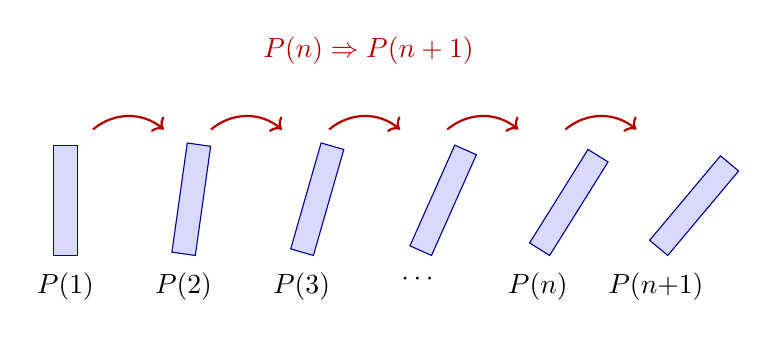
\begin{tikzpicture}[scale=1]
  \foreach \i in {0,1,2,3,4,5} {
    \draw[fill=blue!15,draw=blue!60!black,rotate around={-\i*8:(\i*1.5+0.3,0)}] (\i*1.5,0) rectangle (\i*1.5+0.3,1.4);
  }
  \foreach \i in {0,1,2,3,4} {
    \draw[->,thick,red!70!black] (\i*1.5+0.5,1.6) to[bend left=40] (\i*1.5+1.4,1.6);
  }
  \node[below] at (0.15,-0.1) {$P(1)$};
  \node[below] at (1.65,-0.1) {$P(2)$};
  \node[below] at (3.15,-0.1) {$P(3)$};
  \node[below] at (4.65,-0.1) {$\cdots$};
  \node[below] at (6.15,-0.1) {$P(n)$};
  \node[below] at (7.65,-0.1) {$P(n{+}1)$};
  \node[above,red!70!black] at (4,2.3) {$P(n)\Rightarrow P(n+1)$};
\end{tikzpicture}

\small 数学的帰納法のドミノ倒し：最初が倒れ（$P(1)$）、$P(n)$が$P(n+1)$を倒すなら、全てが倒れる
\end{center}

\section{原著の日本語訳}
数学科学その可能性自体が、不可解な矛盾であるように思える。もし数学科学がただ推論の外見に過ぎないとしても、全員が認めるほど完璧な厳密性はどこから来ているのか？逆に、数学が述べるすべての命題が形式的論理の規則によって順序立てて導き出されるとしても、なぜ数学が巨大な自明の真理の羅列にならないのか？

三段論法は何か新しいことを教えることができない。もし全てが同一性の原理から派生するなら、すべてはその原理に帰着されなければならない。それでは、多くの巻物に記された定理の命題はすべて、AはAであるという間接的な言い換えではないのか？

もちろん、これらの議論の源流にある公理を参照することができます。もし公理が矛盾の原理に還元できないと感じられ、それらが数学的必然性に関としない実験的事実であると見なされるなら、まだ一つの手段があります：その公理は先験的な合成的観念として分類できるというものです。

しかし、これは困難を解決するものではなく、ただその名前を付けるだけです。そして、合成的観念の性質が私たちにとってもう秘密のないとしても、矛盾は消え去ることはありません。それはただ避けられるに過ぎません。三段論法はとえられたデータに対して何か新しいことを教えることができません。データは公理に帰着され、それらが結論にあるすべてです。

定理が新しくなるためには新たな公理が必要でなければなりません。推論は直接的直感から得られる明確な真実をただ借りてくるものでしかありません；それはただ中間的な寄生虫に過ぎません。したがって、三段論法の装置が私たちが借入したものを隠蔽する役割しかないことを疑問視するのは正当ではないでしょうか？

矛盾は数学の本を開くとより鮮明になります。どのページでも著者は既知の命題を一般化することの意図を告白しています。数学的方法は特定から一般へ進むものか、そしてもしそうであるなら、なぜそれが推論的と呼ばれるのか？

数学的推論の本質。

最後に、数の科学が単なる分析的であり、または少数の合成的直感から推演的に導き出されるものであるなら、その科学全体の真理を一度の視覚的な洞察で全知全能な心ではっきりと理解できるように思われるべきです。さらに言えば、これらの真実は誰でも普通の知性を持つ人間にも明白に示されるような言語がいつか発明されることさえ期待できるかもしれません。

これらの推論結果が否認されようと如何ともしがたいですが、数学的な推理には自己で創造的な力があるという点からして、それは三段論法とは区別すべきです。その違いは深いものであることが明らかです。例えば、同じ一様な操作を二つの等しい数に適用しても結果が同一になるという規則の頻繁な使用を見つけることは、この謎の鍵ではないでしょう。これらのすべての推理方法は、三段論法に帰着できるか否かに関わらず、分析的な性格を保持し、その力も失われます。

II.

この議論は古くから存在しています。レーニッツが二加二が四であることをどのように示そうとしたかを見てみましょう。数1を定義し、またとえられた数xに1を加えるという操作a'+iを仮定します。これらの定義はその後の推論には関係ありません。次に、2, 3, 4を以下のように等式で定義します：

(i) 1 + 1 = 2;(ii) 2 + 1 = 3;(iii) 3 + 1 = 4

同様に、操作x+2を次の関係で定義します：(iv) x+2 = (x+1)+1.

これに基づいて：

2 + 2 = (2 + 1) + 1; （定義 iv）(2 + 1) + 1 = 3 + 1; （定義 ii）3 + 1 = 4; （定義 iii）

従って、2 + 2 = 4。証明終了（Q.E.D.）。

以下の文を忠実に日本語に翻訳します：

この論理は純粋に分析的であることは否定できません。しかし、数学の専門家に尋ねれば、「これは真の証明とは呼ばないべきもの；これは検証に過ぎない」と答えるでしょう。私たちは一方の定義と他方の定義を結びつけただけであり、その同一性を検証したに過ぎません。何も新しいことは学べません。検証は証明とは異なるのは、それが分析的であるからで、そして何の進展も生み出さないからです。なぜなら結論は前提の言語を変換しただけだからです。一方、真の証明は果実あるものであり、結論は前提よりも感覚的にはより一般的なものとなります。等式2 + 2 = 4は検証可能であるのは特定の事例だからです。数学における個々の命題は同じ方法で常に検証可能です。しかし、もし数学がこのような検証の一連の系列に過ぎたなら、それは科学ではなくなります。チェスプレイヤーが一枚の駒を獲ることで科学を作り出すわけではありません。科学は一般性を持つもののみが構成します。厳密な科学の目的はこれらの直接的な検証を避けることかもしれません。

数学的論理の本質. 5

III.

次に、幾何学者がどのように働くかを見てみましょう。そしていくつかの彼の方法を驚かせる試みを行いましょう。この作業には困難があります；たまたま一冊の書籍を開き、その中から任意の証明を分析するだけでは不十分です。まず最初に、幾何学を除外しなければなりません。なぜなら、公理の役割、空間概念の性質と起源に関連する難問が混ざることで問題が複雑化します。同様な理由から、無限小解析も利用できません。数学的な思考は純粋な場所を探さなければなりません—すなわち、算術に限られます。しかしまだ選択が必要です；数論のより高度な部分では原始的な数学的概念が非常に深い発展を遂げており、それらを分析することが難しくなります。

算術の初めに、我々が求めている説明を見つけることができるでしょう。しかし、古典的な論文の著者は、最も基本的な定理の証明において特に正確性と厳密さを欠いていることがわかります。彼らに対してこの欠如を罪とするべきではありません；それは彼らが従う唯一の必要条件だからです。初学者は真の数学的厳密さに対応できませんし、それを見ればただ空虚で退屈な細部だけだと感じるでしょう。初学者にその厳密さを求めることは無駄であり、科学の発展を築いた先駆者たちがゆっくりと歩んだ道を素早く通過する必要があります。

なぜこのような長い準備が必要なのか、自分自身にこの完全なる厳密さに慣れるためには、それが自然にはすべての心に課されるべきであるように思えるのに。これは論理的かつ心理学的な問題であり、その研究価値は高いでしょう。しかし、それについては触れません；それは私たちの主題とは外れます。私が強調したいのは、基本定理の証明を再構築し、初学者が疲れるための粗雑な形式ではなく、熟練した幾何学者が満足する形式でそれをとえることだけです。

加法の定義。

x+iという操作が既に定義されていると仮定します；これはとえられた数xに数iを加えることを含みます。この定義について何らかの議論があったとしても、それは後の議論には関係ありません。

次に、任意のとえられた数xに数aを加える操作x+aを定義する必要があります。もし+(-1)という操作が既に定義されていると仮定すると、x + aは等式 (i) x + a = [x + (a - 1)] + iによって定義されます。x + \{a - 1\}の値を知ればx + aの値も分かりますし、私は最初からx+iの値が分かっていると仮定したので、x + 2, x + 3等の操作を順次「帰納的に」定義することができます。この定義は一瞬だけ注意深く検討すべきです。

数学的論理の性質。7

注意点；これは特定の性質を持ち、この段階でも単なる論理的定義とは異なるものである。実際、等式（i）には無数の異なる定義が含まれており、そのそれぞれは先祖の意味を知る限り一つの意味を持つ。

加法の性質。

結合律。—私はa-j-(b--c) = (a-b)--cであることを主張する。実際、この定理はc=iの場合に真であることが明らかである。従って、等式を書き換えるとa-\}-\{b--i) = \{a--b)--iとなる。これは、記号の差異を考慮すると、私が加法を定義した等式（i）と同じである。定理がc=yの場合に真であると仮定し、c=y+1の場合にも真であることを主張する。[(a+è)-f7=a+(6+y)から] [\{a + b) + y]+i=[a + (b + y)]-hiとなり、または定義（i）により—\{a + b) + (7+ i) = a + (6 + y + i) = a + [6+ (7+ i)]。これは純粋な論理的推論によって定理がc=y+1の場合にも真であることを示す。c=iの場合に真であるから、次々とc=2, c=3なども真であることがわかる。

交換律。（i）私はa + i = i-\{-aであることを主張する。この定理は明らかにa=iの場合には真である。純粋な論理的推論によって、もしa=yの場合に真であればa=y+1の場合にも真であることも確認できる。定理がa=iの場合に真であるから、次々とa=2, a=3なども真であることがわかる。これは「帰納法」による証明という意味である。

（2）私はa + b = b + aであることを主張する。この定理はb=iのときにはすでに示されているので、b=yの場合に真であればb=y+1の場合にも真であることも純粋な論理的推論によって確認できる。従って、定理は帰納法により証明される。

乗法の定義。

乗法を次のように等式で定義する：（i）aXi=a。（2）aXb=[aX\{b-ï)]--a。これらのいずれも無数の定義を含み、Xiが定義されたら、次々とax 2, axなどと順に定義できる。

乗法の性質。

分配律。—私は（a--b)Xc = (aXc) + (bxc)であることを主張する。純粋な論理的推論によって、この定理がc=iの場合には真であることが確認できる。次に、もしこの定理がc=yの場合には真であればc=:y+1の場合にも真であることも確認できる。従って、定理は帰納法により証明される。

交換律。——(i) 私は、aXi = Xi aについて述べる。この定理は、a = iの場合に明らかである。もしもa = aのときには真であることが分析的に確認できれば、a = a + 1のときにも真となることが確認できる。

(2) 私は、axb = bxaについて述べる。この定理は、b = iの場合に証明されたばかりである。もしもb = fのときには真であることが分析的に確認できれば、b = f + 1のときにも真となることが確認できる。

IV.

これほど単調な論理展開を今後一時的に置き去りにすることができるが、その単調さこそが、一貫した過程を鮮明に示す。この過程は帰納法による証明である。まず、定理がn = 1のときには真であることを示し、次に、もしもn - 1のときには真であることがあれば、nのときにも真となることを示し、それからすべての整数に対して真であると結論付けることができる。我々は、加法と乗法の規則を証明する方法として、この過程がどのように使用されたかを見た。これは代数学的計算の規則であり、単純な三段論法よりも多くの異なる組み合わせに適応できる分析的な道具である。しかし、それは新たなことを教える能力は全くない。もし数学に他の工具がなければ、その発展は即座に止まってしまうだろうが、同じ過程——すなわち帰納法による論理を再び用いることで、その前進は継続することができる。そして、よく観察すれば、この論理の形態は我々が先ほど示した単純な形式であれ、多少変形された形であれ、各段階で見ることができる。これは数学的な論理の極めて重要なものであり、より詳細に検討する必要がある。

V.

再帰的論理の根本的な特徴は、その中に無数の三段論法が凝縮されていることにあると言える。この点を明確にするために、個々の三段論法を一列に述べることで理解しやすくなるだろう。これらの三段論法は、 cascade（cascade）と表現してもよさそうだ - 連続して続く形で並ぶ。

以下が仮定的三段論法である：- 定理が数 \( i \) に対して真である。- したがって、もし定理が \( i \) に対して真であるなら、それは \( 2 \) も真である。従って、定理は \( 2 \) に対して真である。- さらに、もし定理が \( 2 \) に対して真であるなら、それは \( 3 \) も真である。従って、定理は \( 3 \) に対して真である。- そして、このように続けていく。

私たちは各三段論法の結論が次の三段論法の小前提として使われていることを確認できる。さらに、我々のすべての三段論法の大前提は単純な形に帰着されることがわかる。もし定理が \( n - 1 \) に対して真であるなら、それは \( n \) も真である。

したがって、再帰的論理においては、最初の三段論法の大前提と一般化された公式のみを述べることで十分である。この無限列の三段論法は、数行にまとめられる。

これにより、定理の特定の推論が純粋な解析的手法によって検証可能であることが容易に理解できる。たとえば、すべての数に対して真であることを証明する代わりに、定理が数 \( 6 \) に対して真であることを示すだけであれば、cascade の最初の五つの三段論法を立証すれば十分である。数 \( 10 \) に対して真であることを証明したい場合は、\( g \) 個の三段論法が必要となる。より大きな数に対してはさらに多くの三段論法が必要となるが、どんなに大きな数でも到達できるし、解析的手法による検証は常に可能である。

しかし、どんなに遠くまで行っても、すべての数に対して適用される一般化された定理にはたどり着けない。それが科学の対象であるだけだ。その一般化された定理を達成するためには無限の三段論法が必要であり、分析者の忍耐力は形式論理の資源に制限され、その無限の abyss（断崖）を越えることは決して不可能である。

数学的論理の性質 II

私は最初に、一瞬で数学の全体的な真実を把握する力のある心はなぜ思い浮かばないのかと尋ねました。その答えは容易です。チェスプレイヤーは四手や五手先まで組み立てることができます；しかし、いかに優れたプレイヤーであっても、それ以上の手数を予測することはできません。彼が算術に適用したとしても、直接的直感だけでは一般の真理を思い浮かべることができません；最小限の定理を証明するためには帰納法を使用しなければなりません。これが有限から無限へと移行する唯一の道具です。

この道具は常に有用であり、我々が希望する何らかの段階を一気に飛躍することが可能になります。長い、退屈で単調な検証作業から自由になることができます；これらは速やかに実践的ではなくなります。そして、一般の定理を取り扱うときにはこの道具が欠かせなくなります；それ以外では常に分析的な検証に近づく一方で、それを達成することはありません。

算術のこの領域においては、微分積分学における無限小分析から遠く離れていると感じられるかもしれません。しかし数学的無限という概念が既に支配的な役割を果たしています；なければ何らかの科学も存在しないでしょう；なぜならそれが一般性を持たないからです。

VI.

以下の文を忠実に日本語に翻訳します：

帰納法による論理の基礎となる視点は、他の形で表現することができます。例えば、有限な異なる整数の集合において、常に一つは他のすべてよりも小さいということが言えます。一つの命題から別の命題へと移行し、そうすることで帰納法が正当であるかのような錯覚を抱くことができます。しかし、最終的には止まることになり、結局は証明できない公理に到達します。その公理は、根本的には証明すべき主張を別の言語に翻案したものです。従って、帰納法による論理の規則が矛盾原理に還元されることが不可能であるという結論には逃れられません。また、この規則は実験からも得られません。実験は例えば最初の十個や百個の数について規則が真であることを教えてくれますが、無限の数列全体を教えることはできません。それらは常に有限な部分に留まります。

もしこれが唯一の問題であれば、矛盾原理だけで十分であり、任意の数多くの三段論法を開発することができました。しかし、無数の三段論法を一つの公式で包み込む必要がある場合、この原理は機能しなくなりますし、実験もその助けにはなりません。この規則は分析的証明や実験にアクセスできないものであり、先験的な合成直感の正確な型です。他方で、これは幾何学の公理の場合のように、それが約束事として見られるわけではありません。

なぜなら、この視点が私たちに不可避的に押しつけられる理由は何か？それは一度可能となった行為を無限回繰り返すことができるという心の力の肯定であるからです。心にはその力を直接的に直感し、実験はそれを機会として用いることによって自己認識を得るだけです。

しかし、帰納法による論理の正当性が単なる実験によって確立できないとしても、推引を補う実験はそのような正当性を持つのでしょうか？数々の事例で定理が真であることが確認されると、法則は明白であり、それは非常に多くの観察に基づく物理法則と同じ理由からです。

私たちはここで通常の帰納法過程と類似した明確な類似性を指摘せざるを得ません。しかし、重要な違いがあります。物理学における推引は常に不確定であるため、それは宇宙の一般的な秩序に対する信頼に基づいており、その秩序は私たちに外部からとえられています。一方で、数学的帰納法すなわち再帰による証明は、私自身の性質を肯定するものであり、従って強制的に適用されるべきです。

科学と仮説 14

第七章

私は以前にも述べたように、数学者たちは獲得した命題を一般化することに常に努めます。具体的な例として、私たちは等式 \(a + 1 = 1 + a\) の等価性を示し、それを用いてより一般的な等式 \(a + b = b + a\) を証明しました。したがって、数学は他の科学と同様に、特定から一般へと進むことができます。この事実は、我々が最初にこの研究で不思議に感じたことでしたが、再帰による証明と通常の推引の類似性を確認した後では、もう何ら神秘的な要素はありません。

数学的再帰論理と物理的推引は異なる基礎に基づいていますが、平行線を追って同じ方向へ進むものであり、それは特定から一般への移行です。

このケースをさらに詳しく見ていきましょう。

等式 \(a + 2 = 2 + a\) を証明するには、規則 \(a + 1 - 1 + a\) を二回適用し、\(a + 2 = a + 1 + 1 = 1 + a + 1 = 1 + 1 + a = 2 + a\) と書き換えるだけで十分です。

以下が原著英文の忠実な日本語翻訳です：

従って、純粋に解析的手法によって導き出された等式は単なる特別な例ではなく、全く異なるものである。したがって、数学的論理の真正な分析的・推論的な部分において、「一般から特殊へ」という一般的な意味での進展とは言えないとまで言うことはできない。

等式（2）の両辺は、等式（1）の両辺よりも複雑な組み合わせであり、解析はこれらの組み合わせを要素に分解し、その関係性を研究するだけである。

したがって、数学者は「構築」によって進展を遂げる。「より複雑な組み合わせ」を作り出す。これらの組み合わせや集まりを分析し、原始的な要素に分解すると、要素同士の関係を見出し、それ自体の集まりの関係も導き出すことができる。この過程は純粋に解析的であるが、一般から特殊へという一般的な意味での進展ではない。なぜなら、集まりは明らかにその要素よりも特定的とは考えられない。

「構築」プロセスに対する重要な意義は正しく認識されており、一部の者はそれが正確な科学の発展の必要かつ十分な条件であると主張する。確かに必要だが、十分ではない！有用でない限り、ただの精神労働の無駄であり、より高度な進歩への一歩として役立つためには、まずその構築が要素よりも何かを超越したような統一性を持つべきである。正確に言えば、構築自体を考える方が要素自体よりも有利であるという利点があるべきである。この利点は何なのか？例えば、常に三角形に分解できる多角形について論じる代わりに、基本的な三角形について論じる理由は何か？それは、多角形にはその要素よりも固有の性質があるからである。

任意の辺数を持つ多角形について論じ、それらは特定の種類の多角形に即して適用できる。多くの場合、これらの性質を直接三角形間の関係を研究することで発見するには長い努力が必要である。四角形が単なる二つの三角形の並置を超えるものであればあるほど、それは多角形の種類である。

構築は他の類似の構築と並べて配置されるときだけ興味深いものとなる。これを行うためには、特定から一般へと逆行するか、あるいは一歩または複数の段階を上ることでなければならず、これは必ずしも下降することを強制しない解析的手法「構築による」過程である。しかしながら、我々は数学的帰納法によってのみ昇華できる。これこそが新たな知識を得る唯一の方法だからである。この帰納法に無ければ、物理的帰納法と似ても似つかないが同様に豊かな成果をもたらすものとして機能しない限り、構築は科学を創造する力を持たない。

結論として、私は指摘しておくが、この帰納法は同じ操作が無限に繰り返されることが可能である場合のみ実現できる。これがチェスの理論が科学になることは決してない理由であり、同一の駒の異なる移動は制限され、互いに類似しないからである。

\section{高校生のための解説講義}
\begin{lecturebox}
こんにちは！数学や物理の不思議な世界へようこそ。今日は、皆さんが普段「当たり前」だと思って解いている数学の「証明」の裏側に隠された、非常に深く、そしてエキサイティングな哲学的な謎について一緒に探求していきましょう。

今日のテーマは\textbf{「数学的推論の正体」}です。
「2+2=4」という事実は、ただの計算の結果なのか？ それとも、私たちの脳が新しい真理を「創造」しているのか？

教科書には載っていない、数学の「魂」に触れる講義を始めます。

\subsection*{1. 「検証」と「証明」の決定的な違い}

まず、皆さんに一つ問いかけたいことがあります。
\textbf{「計算すること」と「証明すること」は、同じことでしょうか？}

例えば、以下の手順を見てください。
\begin{itemize}[leftmargin=2em]
\item $1+1=2$ と定義する
\item $2+1=3$ と定義する
\item $3+1=4$ と定義する
\item $x+2 = (x+1)+1$ というルールを決める
\item これらを使って $2+2 = (2+1)+1 = 3+1 = 4$ を導く
\end{itemize}

これは完璧な論理です。しかし、数学の専門家はこれを\textbf{「証明」とは呼ばず、「検証（Verification）」と呼びます。}

なぜなら、この操作は\textbf{「分析的（Analytic）」}なものだからです。
「分析的」とは、\textbf{「結論の中に、すでに前提となる情報がすべて含まれている」}状態を指します。つまり、この計算は「AはAである」という当たり前のことを、少し複雑な言葉に書き換えただけで、新しい知識を一つも生み出していないのです。

\textbf{【図解イメージ：翻訳と検証】}
\begin{itemize}[leftmargin=2em]
\item \textbf{検証：} 「こんにちは」を英語に訳して「Hello」と言うこと。言葉が変わっただけで、新しい情報は増えていません。
\item \textbf{証明：} 「こんにちは」という挨拶から、新しい「友人の輪」という概念を導き出すこと。
\end{itemize}

数学における\textbf{「真の証明」}とは、前提よりも\textbf{「感覚的により一般的なもの」}を導き出すことなのです。

\subsection*{2. 数学的帰納法の「創造性」}

では、数学はどうやって「新しいこと」を生み出しているのか？
ここで、皆さんが数学IIやIIIで習う\textbf{「数学的帰納法」}を、哲学的な視点から再定義してみましょう。

通常、帰納法はこう教わります：
\begin{itemize}[leftmargin=2em]
\item $n=1$ で成り立つことを示す。
\item $n=k$ で成り立つと仮定し、$n=k+1$ で成り立つことを示す。
\end{itemize}

しかし、このプロセスには\textbf{「創造的な飛躍」}が含まれています。
なぜなら、私たちは「$k$ という特定の数」から「$k+1$ という次の数」へ進むための\textbf{「操作（ルール）」}を定義しているからです。

\paragraph{ステップごとの数式展開：加法の定義}
講義のテキストにある「加法の定義」を、高校数学の視点で再構築してみましょう。

私たちは「$x+a$」という操作を、以下のように\textbf{帰納的に}定義します。

$$x + a = [x + (a - 1)] + 1 \quad (\text{ただし } a > 1)$$

この式を見てください。これは単なる計算式ではありません。
「$a$ を足す」という行為を、「$a-1$ を足したあとに、さらに $1$ を足す」という\textbf{構造的なステップ}に分解しています。

このとき、私たちは\textbf{「加法の性質（結合律）」}を証明しようとします。
$$a + (b + c) = (a + b) + c$$

これを証明する際、私たちは「$c=1$ のとき」をチェックし、次に「$c=y+1$ のとき」を考えます。
ここで重要なのは、\textbf{「$y$ で成り立つなら、$y+1$ でも成り立つ」という「構造の継承」}を見抜くことです。

\textbf{【直観的解説】}
帰納法は、ドミノ倒しのようなものです。
「最初のドミノが倒れること」と「一個倒れたら次も倒れるというルール」を証明することで、\textbf{無限に続くドミノの倒壊という「巨大な真理」を、一瞬の洞察で掴み取っている}のです。これが「分析」を超えた「創造」の瞬間です。

\subsection*{3. 「公理」と「直観」：数学の源泉}

ここで、少し難しい言葉が出てきます。\textbf{「ア・プリオリ（先験的）な合成判断」}。
難しく聞こえますが、高校生のみなさんにはこう説明します。

\textbf{「私たちの脳が、経験する前にすでに持っている、世界を組み立てるための『直観的なルール』」}のことです。

数学の定理は、この「直観的なルール（公理）」から、論理の鎖（三段論法）を使って導き出されます。
しかし、三段論法自体は「新しいこと」を教えません。三段論法は、\textbf{「公理という種から、定理という花を咲かせるための『道筋』を整える装置」}に過ぎません。

\begin{itemize}[leftmargin=2em]
\item \textbf{公理：} 種（直観的な真理）
\item \textbf{三段論法：} 成長のプロセス（論理的な推論）
\item \textbf{定理：} 花（導き出された新しい知見）
\end{itemize}

もし、数学がただの三段論法（分析）だけで構成されているなら、数学は「巨大な自明の真理の羅列」になってしまいます。しかし、数学が私たちを感動させるのは、\textbf{「公理から、私たちの想像を超えた一般性を導き出す創造的な力」}があるからです。

\subsection*{4. まとめ：数学を「感動」として捉えるために}

今日の講義の核心をまとめましょう。

\begin{itemize}[leftmargin=2em]
\item \textbf{検証は「翻訳」である：} $2+2=4$ を定義から導くのは、単なる言葉の変換であり、新しい発見ではない。
\item \textbf{証明は「創造」である：} 帰納法や一般化によって、特定の事例から「普遍的な法則」を導き出すことこそが数学の真髄。
\item \textbf{推論は「寄生虫」である：} 厳密に言えば、論理的な推論は「直観的な真理」に寄生して動くもの。しかし、その推論の鎖が完璧であるからこそ、私たちは巨大な真理に到達できる。
\end{itemize}

\textbf{【最後に：君たちへのメッセージ】}
次に数学の証明を解くとき、ただの「計算の作業」としてこなさないでください。
その数式の裏側には、\textbf{「人間の直観が捉えた世界の構造を、論理の力で巨大な真理へと拡張しようとする、人類の知性の冒険」}が隠れています。

数式を「解く」のではなく、数式が描く「真理の風景」を「見よう」としてみてください。それが数学を、ただの教科書から、魂を揺さぶる芸術へと変える第一歩です。

\textbf{【用語解説】}
\begin{itemize}[leftmargin=2em]
\item \textbf{分析的（Analytic）：} 結論の中にすでに前提が含まれていること。
\item \textbf{合成的（Synthetic）：} 前提にはない新しい要素や概念を組み合わせて結論を導くこと。
\item \textbf{三段論法（Syllogism）：} 「A=B、B=C、ゆえにA=C」という推論形式。
\item \textbf{公理（Axiom）：} 証明なしに正しいと認める、数学の出発点となるルール。
\end{itemize}
\end{lecturebox}


\clearpage
\chapter{数学的量と経験}
\begin{center}\large\textit{物理的連続体と数学的連続体、実数の切断、デデキントの連続性公理、測定と感覚の閾値}\end{center}

\section*{この章の見取り図}
\begin{center}

\begin{tikzpicture}
  \draw[->,thick] (-0.5,0) -- (10.5,0);
  \foreach \x/\l in {0/0,2.5/1,5/2,7.5/3,10/4} { \draw (\x,0.1)--(\x,-0.1) node[below]{$\l$}; }
  \fill[blue!25] (0,0.15) rectangle (4.1,0.5);
  \fill[red!25] (4.1,0.15) rectangle (10,0.5);
  \draw[very thick,green!50!black] (4.1,-0.5)--(4.1,1.3);
  \node at (2,0.85) {集合 $A$ ($x^2<2$)};
  \node at (7,0.85) {集合 $B$ ($x^2>2$)};
  \node[green!50!black,above] at (4.1,1.3) {切断：$\sqrt2$};
\end{tikzpicture}

\small デデキントの切断：数直線を二つの集合 $A$, $B$ に分ける切れ目が実数を定める
\end{center}

\section{原著の日本語訳}
数学の連続性について数学家が何を意味しているかを知りたいのであれば、幾何学に頼るよりも無駄である。幾何学者は常に、よりまたはそれほど少ない程度で、彼が研究する図形を自己表現しようと試みているが、その表現は彼にとってただの道具であり、空間は彼の幾何学において chalk と同じように使用されるものに過ぎない。そして、 chalk の白さのような偶然性はしばしば重要な要素ではない。

純粋な解析学者にはこのような罠から心配する必要はない。彼は数学をすべての外的な要素から解放し、我々の質問に答える立場にある：「この連続性について、数学家が論じているのは何なのか、詳しく教えてくれ」。多くの思考深い解析学者たちは既にそのような問いかけを行っている。例えば、Tannery は彼の『関数論入門』においてそうしたことをしている。

我々は整数から始めよう。連続する任意の二つの集合間に一つ以上の中間的な集合を挿入し、それらの集合間にさらに他の集合を挿入し、無限に繰り返す。これにより無限の項が得られ、これらは分数、有理数、または共通比の数と呼ばれる。

しかし、まだ全てではない；これらの項は既に無限個存在するにもかかわらず、さらに他の項が挿入される。これらは無理数または不共通比の数と呼ばれる。

さらに進む前に、事前の注意を述べておきたい。このように考えられた連続体は、個々の要素が特定の順序で並べられた無限集合ではなく、互いに独立しているものである。これは通常の概念とは異なり、要素間には密接な関係があり、それが一つの全体を作り出すという考え方ではない。点が線よりも前に存在するのではなく、線が点よりも前に存在するという考えも含まれていない。唯一残るものは多様性であり、統一は失われている——「連続体は多様性の中の統一」であるという有名な公式通りだ。解析学者たちは、このように定義すること自体に誇りを持っているが、実際には常にそのような連続体に基づいて論理を展開している。読者に注意を促すだけでも十分だが、数学的な連続体は物理学者や形而上学者のそれとは全く異なるものである。

また、おそらく言えるのは、この定義に満足する数学者たちは言葉の罠に陥っていることだろう。これらの集合それぞれの性質を正確に示すべきであり、どのようにこれらが配置されるかを説明し、それが可能かどうかを示すべきである。しかし、これを行う必要はないとするのも誤りだ。論理展開において重要なのは、他のどの集合よりも前に存在することやそれらの後ろにあることという性質だけである。したがって、これらの集合がどのように配置されるかについては気に留めないでよいし、その操作の可能性について疑問を持つ人はいないだろう。ただし、「可能」という言葉は幾何学者の言葉では矛盾なしであることだけを意味するからだ。しかし、私たちの定義はまだ不完全であり、この長い説明の後で再びそれを扱う必要がある。

無比数の定義。ベルリン学派の数学家たち、特にクロネッカーは、整数のみを使用して無理数や分数を含む連続な尺度を構築しようと努力しました。この視点から見れば、数学的な継続性は純粋に心の創造であり、実験には関としないものであるでしょう。

有理数の概念が彼らにとって何らの困難も感じられなかったとしても、クロネッカーたちは主に無比数を定義することに焦点を当てました。しかし、その定義をここで再現する前に、読者の中にはこの定義が引き起こす驚きを和らげるための一言が必要です。数学的な研究は物体自体ではなく、物体同士の関係性に焦点を当てるのです。彼らはこれらの物体が他に置き換えられても構いませんし、関係性が変わらない限り、物質そのものには興味はありません。形式だけに注目します。

もし私たちがそれを忘れてしまっていたら、無比数という名前を単なるシンボルにとえることの意味を理解するのが困難かもしれません。つまり、測定可能な量として我々が持つべき概念とは全く異なるものです。

ではクロネッカーの定義を見てみましょう。互いに比で測れる数は無限の方法でクラス分けすることができます。ただし、どのクラスの任意の数も他のクラスのどの数よりも大きいという条件があります。例えば、第一クラスにはすべて2より大きな数と2そのもの、第二クラスにはすべて2未満の数を含めるとします。この場合、2は第一クラスの中で最小の数となります。したがって、2はこの分類のシンボルとして選ぶことができます。

逆に、第2のクラスの中に全ての他の項よりも大きいものがある場合があります。例えば、第1のクラスがすべて2より大きな数で構成されている場合、そして第2のクラスが2未満のすべての数と2そのものを含む場合、この状況は発生します。また、この分類においても、数字2をこの分類の象徴として選ぶことができます。

しかし、どちらのクラスにも、全ての他の項よりも小さいものがない場合もあります。例えば、第1のクラスにすべて平方が2より大きい数を、そして第2のクラスにすべて平方が2未満の数を配置する場合を考えます。我々は明らかに、いずれのクラスにも平方が2である数は存在しないことを知っています。このような状況では、第1のクラスには全ての他の項よりも小さいものが存在しないことが明白です。なぜなら、任意の数字の平方が2に近いかどうかに関係なく、常により近い平方を持つ有理数を見つけることができます。

クロネッカーの見解からすると、無理数√2はこの特定の有理数の分類方法の象徴です。それぞれの分類方法に対応する、無理数や有理数であるような数がこのような形で存在します。しかし、これらの象徴に具体的な存在を付とすることについて満足することは、その起源を忘れるものであり、それらの象徴がどのようにして具体的な存在として認識されたかを説明する必要があります。また、分数の難題はここから始まらないでしょうか？我々がこれらの数の概念を持つのは、無限に分割可能な物質があると我々が理解しているからではないでしょうか、すなわち、連続体と考えるからではないでしょうか？

物理学的連続体。——次に、数学的な連続体の概念が単に実験から導き出されたものではないかと問うてみる。もしそれがそうであるなら、実験で得られる粗雑なデータ、すなわち感覚は測定可能であると考えたくなるだろう。最近ではそのような試みがあり、さらにはフェンナーの法則という名前の法則が提唱され、刺激と感覚との関係は対数的比例であると述べられている。しかし、この法則を確立するために行われた実験を検討すると、全く反対の結論に至るだろう。例えば、10グラムの重さAと11グラムの重さBが同一の感覚を生むこと、重さBは12グラムの重さCから区別できなくなる一方で、重さAは重さCから容易に区別できることが観察されている。したがって、これらの実験の結果は以下の関係式で表現される可能性がある：A = B, B = C, A < C。これらは物理学的連続体の公式とみなすことができる。

しかし、この法則に対する矛盾律に反する不可容許な不一致があり、この不一致を排除する必要性から数学的な連続体という概念が創造された。したがって、我々は結論を導き出す：この概念は完全に心で生み出されたものであるが、それは実験がその機会をとえたのである。我々は三つの量が第三の量と等しいときには互いに等しくないという信じられないような考えを抱くことはできないため、AはBとは異なるし、BはCとは異なると考えざるを得ない。そして、これが明らかでなかったのは、私たちの感覚の不完全性によるものであると考えられる。

数学的連続体の創造：第一段階。——これまで、事実を説明するために、AとB間に区別できないほど少ない数の項を挿入すれば十分でした。しかし、感覚の弱さを補うために何か装置を使用する場合、何が起こるでしょうか？例えば、顕微鏡を使用する場合、以前は区別できなかったAとBも今では区別できるように見えます。しかし、AとBという異なる項間に新たな項Dが挿入され、このDはAからもBからも区別できないことがわかります。いかに精密な方法を使っても、実験の粗い結果には物理的連続体固有の矛盾が残ります。これを回避するためには既に区別された項間に新たな項を無限に挿入し続ける必要があります。

私たちは、物理的連続体を離散的な要素に分解できる十分強力な装置を想像できれば、この操作を停止できると考えることができるかもしれません。望遠鏡が Milky Way を星々の集合体として分解するようにです。しかし、これも想像することはできません；私たちの装置は常に感覚器官と共に使用されます。顕微鏡によって拡大された像は眼で観察され、その結果、この像には視覚的な知覚の特性が残り、それらは物理的連続体の特性を保持します。

直接観測された長さと、顕微鏡によって二倍に拡大された半分の長さとは区別がありません。全体は部分と同質であり、そして新たな矛盾が生じます—もしくは、項の数を有限と考える場合にこそ矛盾が現れます；明らかに、より少ない項を持つ部分は全体と類似することができません。この矛盾は、項の数を無限と考えるときには解消します。例えば、整数全体と偶数全体との集合が類似していることを考えることができます—これは整数全体の一部です；実際には、各整数に対応する偶数があり、それがその整数の二倍となります。しかし、この矛盾を避けるためだけではなく、実験データに含まれるこの矛盾から、我々は連続体という概念を作り出すことが促されます。それは無限の項で形成される集合です。

ここでは、整数列の場合と同様に全てが進行します。単位を単位の集まりに追加することができるという能力があります。実験を通じてこの能力を使う機会があり、その存在を認識していますから、我々はその力を無限に拡張できると考えるのです；実際に、それ以上に多くの物体を数える必要がなかったとしてもです。同様に、連続した項の間に新たな項を挿入すると、この操作を無限に続けることができるという感覚があります。つまり、ある内在的な理由で停止する必要がないように思えます。

省略せずにこの操作を継続することが可能であると理解し、名前をつけるために、このような集合を「初等の数学的連続体」と呼びましょう。そして、無理数の法則に従って新たな集合を挿入すると、それが「二階の数学的連続体」呼ばれるものです。

第二段階。—私たちは最初の一歩を踏み出しました。第一階の連続体の起源について説明しましたが、なぜこれだけでは不十分で、無理数が必要だったのかを見なければなりません。

もし線を想像しようとすると、それは物理的な連続体の特性を持つべきである——つまり、我々のイメージには一定の幅があるべきだ。したがって、二つの線は私たちには二つの狭い帯として現れるだろう。そして、この粗雑なイメージに満足する限りでは、明らかに二つの線が交差する場所には共通部分があるべきである。

しかし、純粋な幾何学者はさらに一歩進める。感覚の助けを完全に捨てずに、彼は無幅の線と無寸法の点を想像しようと試みる。彼はこれを行うために、帯が徐々に狭くなる方向へ向かう限界として線を想像し、領域が徐々に小さくなる方向へ向かう限界として点を想像することができる。

どんなに細かい帯であっても、我々の二つの帯には常に共通の領域がある。その領域は帯が小さくなるにつれて小さくなり、その極限が幾何学者が「点」と呼ぶものである。これがなぜ交差する二つの線には共通の点があると述べられるか、そしてこの真実は直感的なものである。

しかし、もし線を最初の階級の連続体と考えると矛盾が生じる——つまり、幾何学者によって描かれた線はただ点をとえ、その座標が有理数である点だけをとえるべきだ。例えば、線と円の存在を主張する場合にそれが明白な矛盾となる。実際、もし座標が共通比的な点のみを考慮すると、正方形の内接円と正方形の対角線は交差しないだろう。なぜなら、交点の座標は共通比的ではないからである。

それでもなお、我々には特定の無比的な数しか存在せず、すべての数が存在しないことになる。

以下、原著英文を忠実に日本語へ翻訳した結果です：

しかし、まず私たちは線を二つの半線分（dcnii-dnnlcs）に分割する状況を想像しましょう。これらのそれぞれの半線分は私たちの心に特定の幅を持つ帯として現れます。これらの帯は隙間なく密着し合うべきであり、そのためには間に隙間が存在してはなりません。共通部分は点として私たちは認識し、その帯を徐々に狭く想像するにつれて、依然として点として残ります。つまり、線を二つの半線分に分割した場合、これらの半線分の共通境界は点であるという直感的な真理として受け入れることができます。ここではクロネッカーの概念が認識されます。

数学的量第27頁

無理数は二つの有理数クラスの共通境界と見なされた、クローンナーの概念において同様に認識されるべきです。これが第二位の連続体、つまり真の数学的連続体の起源です。

要約 — まとめると、心にはシンボルを作成する能力があります。そしてそれはこのようにして数学的連続体を構築しました。そのシンボルシステムは特定のものに過ぎません。その力の唯一の制限は矛盾を避ける必要性だけですが、心は実験がそれを正当化する場合のみ使用します。

私たちが現在考慮しているケースでは、その理由は感覚的な粗いデータから物理的連続体という概念を得ることによってとえられます。しかし、この概念は一連の矛盾を導き出し、それらのうちのそれぞれから解放される必要があります。これにより私たちはますます複雑なシンボルシステムを想像することに強制されます。その中で私たちが焦点を当てるものは、内部矛盾がないだけでなく、さまざまな直感的な命題と矛盾していないことを確認した時点で既にそうであったように、それ自体から内面的矛盾がなくなりました。

測定可能な量 — これまでのところ、我々は量の測度について言及していません。あるものが他のよりも大きいかどうかを判断することはできますが、それが二倍または三倍大きいとは言えません。

この翻訳では、原著の論理と語調に忠実に、かつ自然な日本語で表現しています。文中の数式や変数はLaTeX形式で記述しています。

これまで、項がどのように並べられているかの順序についてのみ考慮してきましたが、これだけでは多くの応用には不十分です。任意の二つの項を分ける区間の大きさを比較する方法を学ぶ必要があります。この条件に従って初めて連続体は測定可能になり、算術の操作も適用されます。これは新しい特別な仮定によってのみ達成できます；その仮定は、項 A と B の間に存在する区間が項 C と D の間に存在する区間と等しいというものです。

例えば、整数から始めましたし、連続した二つの集合の間に n 個の中間的な集合を挿入しました。仮定によってこれらの新しい集合は等距離であると仮定します。これは二つの量の加法を定義する一つの方法です；つまり、区間 AB が定義上区間 CD に等しい場合、区間 AD は定義上区間 AB と AC の和となります。この定義は非常に任意的ですが、完全にはそうではありません。これは加法の交換律や結合律などの一定の条件を満たす必要があります；しかし、選択した定義がこれらの法則を満たす限り、その選択は無関係であり、正確に述べる必要はありません。

補足説明。現在では、以下の重要な問題について議論する立場にあります。

(i) 応用力のある心の創造力は、数学的な連続体の作成によって尽きてしまいますか？答えは否定的で、Dubois Reymond の研究により非常に鮮明に示されます。

私たちは、数学的に異なる階次の無限小を区別することを知っています。無限小の二番目の階次は、絶対的な意味でだけでなく、最初の階次の無限小に対しても無限に小さいです。分数甚至は無理数の階次における無限小を想像することは難しくありませんし、ここでもまた先ほどのページで扱った数学的連続体を見つけることができます。

さらに、最初の階次に対する無限に小さい一方で、任意に小さなeに対して無限に大きい無限小もあります。つまり、我々の数列の中に新たな用語が追加されることになります。そして、もし私が先ほどのページで使用した用語を再び用いることを許していただけるなら、非常に便利な用語でありながら慣習によって承認されていないものですが、私はこのような連続体を第三階次と呼ぶべきだと考えます。

さらに進むことは容易です。しかし、それを行うのは無意味です。なぜなら、そのような符号は実際的な応用がなく、誰もそれを想像することはありません。第三階次の連続体は、異なる階次における無限小を考慮することで導き出されるものですが、その自身の価値は小さく、引用する価値すらほとんどありません。幾何学者たちはこれを見なれの趣味としか考えていません。創造的な思考は実験が必要なときだけに使われるのです。

（2）数学的連続体の概念を得た後でさえ、そのような概念が生じた矛盾類似の矛盾から免れるのでしょうか？いいえ、以下はその例です：

彼は確かに天才である。すべての曲線が接線を持つという事実を疑わない者は、その論理を理解していると言えるだろう。実際、曲線と直線を二つの狭い帯と考えると、常に両者が共通部分を持ちながら交差しないように配置できる。現在、これらの帯の幅が無限に小さくなると仮定しよう。共通部分は依然として存在し、極限状態において、二つの線は共有点を持つことになる。ただし、これらは交差していないのである—つまり接している。このような論理を用いる幾何学者は、二直線が交わるときには共有点を持つという証明で我々自身が行ったことと同様のことを行っているに過ぎないし、彼の直感も正当であるように思えるかもしれない。しかし、そうではない。ある曲線が接線を持たない場合を示すことができる。そのような曲線を二階の解析的連続体と定義すればよいのである。もちろん、上記で述べたような類似の技巧によってこの矛盾を解消することは可能であるが、このような矛盾は非常に稀な例外的なケースにしか現れないので、それを追求する必要はない。直感と分析の調和を試みる代わりに、どちらか一方を犠牲にするべきであり、そして分析が完璧であることを保証するために直感は無視されるべきである。

幾何学的連続体の多次元性について。我々は先に述べたように、直感から得られる物理的な連続体について議論した。もしくは、読者が好むならフェンナーの実験結果から得られた粗略な結果に基づいて述べたと理解してほしい。私はこれらの結果を以下のような矛盾する公式で要約した：A=B, B=C, A<C。

では、この概念がどのように一般化され、多次元連続体の概念が導かれるのかを見てみよう。任意の二つの感覚集合を考える。これらを区別できるか否かは明確である。フェンナーの実験で10グラムと12グラムの重さは区別できるが、11グラムの重さとは区別できない。これが多次元連続体を構築するための必要な条件である。

これらの感覚の集まりの一つを要素と呼びましょう。これは数学的な点に類似していますが、全く同じものではありません。我々は「要素」が大きさがないとは言えないと述べることができます。なぜなら、その要素を直近の隣接要素から区別することはできないためです。したがって、それは一種の霧で包まれているように見えます。天文学者の比較を許すならば、「要素」は星雲に類似し、数学的な点は星に類似します。

この仮定が成り立つ場合、要素の系統は連続体を形成します。もし我々がどの要素からも他の任意の要素へと一連の連続した要素を通じて移動できるなら、それは連続体です。これらの連続した要素はそれぞれ前のものと区別できないとしましょう。この線形系列は数学家の直線に対し、孤立した要素が点に対応します。

さらに進む前に、カットという概念を説明しなければなりません。連続体Cからいくつかの要素を取り除き、一時的にこれらの要素が連続体に属さないと見なすことにしましょう。このような取り除かれた要素の集まりをカットと呼びます。このカットにより、連続体Cはいくつかの異なる連続体に分割されます。残された要素の集まりは単一の連続体ではなくなります。

すると、C上には二つの要素AとBがあり、これらはそれぞれ異なる連続体に属していると考えるべきです。これは不可能ではないでしょうか？なぜなら、C上の線形系列の連続した要素（各要素が前のものと区別できないもので、最初のものはAで最後のものはBである）を見つけることができないからです。この系列の一つの要素がカットの一つの要素と区別できない場合を除いては、そのような線形系列を見つけることは不可能だからです。

逆に、切断が連続体を十分に分割しない場合があるかもしれません。物理的連続体を分類するためには、まずその連続体をどのように切断すれば分割できるかの性質を確認する必要があります。物理的連続体Cが有限個の要素（すべて互いに区別可能）に分割されるような切断によって分割できる場合、私たちはCを1次元の連続体と呼びます。一方で、Cを自身も連続体である切断でしか分割できない場合、私たちはCを複数次元の連続体と呼びます；もし切断が1次元の連続体である場合、私たちはCを2次元の連続体と呼びます；切断が2次元の連続体である場合、私たちはCを3次元の連続体と呼びます。そして如此して下去ることで、物理的複数次元連続体の概念が定義されます。この定義は非常に単純な事実に基づいており、感覚の集合群が区別可能か否かによって決まるからです。

数学的複数次元連続体 — 数学的複数次元連続体n次元の概念は、この章の冒頭で議論したような過程により自然に導き出すことができます。そのような連続体の一点は、その点を定めるn個の異なる量（座標と呼びます）によって定義されます。

以下の文を忠実に日本語に翻訳します：

これらの量は必ずしも測定可能であるとは限らず、例えば、幾何学の一つの分野では、量の測定から独立しており、ここでは、曲線ABC上の点Bが点AとCのどちらか一方にあるかどうかを知ることが主な目的であり、また弧ABが弧BCに等しいかそれの2倍であるかは関係ありません。この分野は「位置解析」と呼ばれます。これは非常に多くの教義を含んでおり、最も優れた幾何学者たちの注目を集めています。そして、これらの教義から一連の驚くべき定理が導き出されます。これらの定理が通常の幾何学の定理と異なるのは、それらは純粋に質的である点です。不慣れな描画によって図形が複製されても、比例関係が歪められたり直線が多少曲がった線で置き換えられても、これらの定理は依然として成り立ちます。

我々が定義した連続体に測量を導入すると、その連続体は空間となり、幾何学が生まれます。しかし、この議論は第2部で扱われます。

第2部。

空間。

\section{高校生のための解説講義}
\begin{lecturebox}
こんにちは！数学と物理の不思議な世界へようこそ。今日は、皆さんが当たり前だと思っている「連続している」という感覚の裏側に隠された、非常にエキサイティングで、少し哲学的な「数学の正体」について一緒に探求していきましょう。

今日のテーマは\textbf{「数学的連続体と物理的連続体」}。
「線はつながっている」という当たり前の感覚が、数学の世界ではどう定義され、私たちの感覚とどう違うのか。原著の深い洞察をもとに、ステップを追って解き明かしていきましょう。

\subsection*{1. 幾何学の「道具」と解析学の「本質」}

まず、皆さんが普段見ている「図形」について考えてみましょう。
例えば、教科書に載っているきれいな円や直線。幾何学者はこれらを描くとき、空間を「チョーク（粉）」のように使います。チョークの白さがどうであれ、重要なのは「形」そのものではなく、その形が持つ性質です。

しかし、\textbf{解析学（数学の連続性を扱う分野）}はもっとストイックです。彼らは「外的な要素（見た目や色、空間の質感）」をすべて排除します。
彼らが問いかけるのはただ一つ。
\textbf{「数学家が言う『連続性』とは、一体何を指しているのか？」}
これに答えるために、私たちは「見た目」を捨てて、純粋な「論理」の海へ飛び込みます。

\subsection*{2. 連続体の構築：無限の「割り込み」}

では、数学はどうやって「連続」を作り出すのか。
まずは、私たちが知っている\textbf{「整数」}からスタートしましょう。

\begin{itemize}[leftmargin=2em]
\item \textbf{第一のステップ：} 2つの整数の間に、中間的な数（分数）を入れます。
\item \textbf{第二のステップ：} その分数と分数の間に、さらに別の数（より細かい分数）を入れます。
\item \textbf{無限の繰り返し：} これを無限に繰り返すと、\textbf{「有理数（分数）」}の集合が得られます。
\end{itemize}

しかし、ここで数学者はこう言います。
\textbf{「まだ、全部ではない。」}

有理数をどれだけ細かく詰め込んでも、その隙間にはまだ「穴」が開いています。その穴を埋めるのが\textbf{「無理数」}です。数学的な連続体とは、有理数という無限の点の間にも、さらに無限の無理数が「割り込んでいる」状態を指します。

\paragraph{【重要】連続体は「並び」ではない！}
ここで非常に重要な注意点があります。
数学的な連続体は、\textbf{「要素を順番に並べたリスト」ではありません。}
「点が線より前に存在するか？」という問いは無意味です。連続体とは、個々の要素が独立していながら、それらが密接に関わり合って一つの「全体」を作り出す\textbf{「多様性の中の統一」}なのです。

\subsection*{3. クロネッカーの挑戦：無理数の「象徴」}

ここで、19世紀の数学者クロネッカーの面白い視点を紹介します。彼は「整数だけを使って、無理数を含む連続な尺度を構築しよう」と試みました。

彼は、数値を「クラス（グループ）」として捉えました。
例えば、$\sqrt{2}$ という数について考えてみましょう。

$\sqrt{2}$ は、有理数の世界では「どこにも存在しない」数です。しかし、クロネッカーはこう考えました。
「$\sqrt{2}$ より小さい有理数のグループ」と「$\sqrt{2}$ より大きい有理数のグループ」がある。この\textbf{2つのグループの境界線（象徴）}こそが $\sqrt{2}$ である。

つまり、数学における「数」とは、物体そのものではなく、\textbf{「関係性（境界）の象徴」}なのです。
私たちが「$\sqrt{2}$」と呼ぶとき、それは具体的な物質を指しているのではなく、\textbf{「この境界線よりも右か左か」という関係性を定義している}のです。

\subsection*{4. 物理的連続体 vs 数学的連続体（ここが感動のポイント！）}

さて、ここからが今日の核心です。\textbf{「私たちの感覚（物理）」と「数学」のズレ}についてです。

\paragraph{物理的連続体の矛盾}
私たちの感覚（感覚の閾値）は、実は\textbf{「不完全」}です。
例えば、重さを測るとき、以下の現象が起こることがあります。
\begin{itemize}[leftmargin=2em]
\item 重さAと重さBは、感覚的に「同じ」と感じる。 ($A = B$)
\item 重さBと重さCは、感覚的に「違う」と感じる。 ($B \neq C$)
\item なのに、重さAと重さCを比べると、感覚的に「同じ」と感じる。 ($A = C$)
\end{itemize}

これは\textbf{矛盾律（$A=B, B \neq C$ ならば $A \neq C$ でなければならない）に反しています。}
なぜこんなことが起きるのか？ それは私たちの\textbf{「感覚の粗さ」}のせいです。私たちの脳は、微細な差を切り捨てて「連続している」と錯覚しているのです。

\paragraph{数学的連続体の創造}
数学はこの「感覚の矛盾」を許しません。
数学者は、この矛盾を解決するために\textbf{「無限の挿入」}という概念を創造しました。

\begin{itemize}[leftmargin=2em]
\item \textbf{顕微鏡の例え：}
\end{itemize}
    最初はAとBが同じに見えた（感覚の限界）。
    顕微鏡を使えば、AとBの間に差があることがわかる。
    さらに高性能な顕微鏡を使えば、AとBの間にさらに別の点Dがあることがわかる。
    \textbf{「いかに精密な装置を使っても、感覚の粗さによる矛盾は消えない」}

\begin{itemize}[leftmargin=2em]
\item \textbf{数学の解決策：}
\end{itemize}
    数学は、この「装置の限界」を突破するために、\textbf{「無限に分割可能な連続体」}という概念を\textbf{「心（論理）」}の中に作り上げました。
    物理的な世界では、どれだけ細かく見ても「粒」や「限界」があるかもしれない。しかし、数学は\textbf{「無限に、無限に、割り込み続けることができる」}というルールを定義することで、物理的な矛盾を克服したのです。

\subsection*{まとめ：講義の結び}

今日の講義のまとめです。

\begin{itemize}[leftmargin=2em]
\item \textbf{物理的連続体}は、私たちの「感覚の不完全さ」によって生み出された、少し矛盾を含んだ「近似」です。
\item \textbf{数学的連続体}は、その矛盾を排除するために、人間の知性が「無限の割り込み」という論理によって構築した、純粋な「理想」です。
\end{itemize}

数学は、私たちの感覚を否定するものではありません。むしろ、\textbf{「私たちの感覚が届かないところまで、論理の糸を伸ばしてくれたもの」}なのです。

次に皆さんが「滑らかな曲線」を見たとき、その裏側にある「無限の割り込み」と、それを支える数学者の「純粋な思考」に思いを馳せてみてください。数学は、私たちの感覚の先にある真理を映し出す鏡なのです。

\textbf{【用語解説】}
\begin{itemize}[leftmargin=2em]
\item \textbf{有理数 (Rational Number):} 分数 $\frac{p}{q}$ （$p, q$は整数）で表せる数。
\item \textbf{無理数 (Irrational Number):} 分数で表すことができない数（$\sqrt{2}$ や $\pi$ など）。
\item \textbf{矛盾律 (Law of Non-contradiction):} 「Aであり、かつAでない」ということはありえないという論理の基本原則。
\item \textbf{デデキントの連続性公理:} 実数直線において、ある点より小さい数と大きい数に分けるとき、その境界に必ず「実数」が存在するという、数学的な連続性の定義。
\end{itemize}
\end{lecturebox}


\clearpage
\chapter{非ユークリッド幾何学}
\begin{center}\large\textit{ロバチェフスキー幾何学（双曲幾何）、リーマン幾何学（楕円幾何）、第五公準（平行線公準）、ポアンカレ円板モデル}\end{center}

\section*{この章の見取り図}
\begin{center}

\begin{tikzpicture}[scale=1.0]
  \draw[thick,fill=blue!5] (0,0) circle (3);
  \draw[thick,blue!70!black] (-3,0) -- (3,0);
  \draw[thick,red!70!black] (-1.5,2.598) .. controls (-0.6,0.5) and (0.6,0.5) .. (1.5,2.598);
  \draw[thick,green!50!black] (-1.5,-2.598) .. controls (-0.5,-0.9) and (0.5,-0.9) .. (1.5,-2.598);
  \fill (-1.5,2.598) circle (1.5pt); \fill (1.5,2.598) circle (1.5pt);
  \node[blue!70!black] at (0.5,0.2) {直線};
  \node at (0,-3.4) {ポアンカレ円板：円周上は無限遠};
\end{tikzpicture}

\small ポアンカレ円板モデル：円周に直交する円弧が「直線」となり、同一直線外の点を通る平行線が無数に引ける
\end{center}

\section{原著の日本語訳}
すべての結論は前提に基づいています。これらの前提は、自明で証明不要なものもあれば、他の命題に基づくものもあります。そして、このような追跡を無限に遡ることは不可能であるため、帰納的科学、特に幾何学には一定数の証明不能な公理が必要です。したがって、すべての幾何学の論文はこれらの公理の明示的な述べ方から始まります。

しかし、これら公理には区別があります。例えば、「同じものに等しいものは互いに等しい」などは幾何学の命題ではなく、分析の命題です。私はこれらを先験的解析的直観と見なし、それらについてはさらに言及しません。しかし、幾何学特有の公理について強調する必要があります。これらのうち、多くの論文では明示的に三つ述べられています：

(1) 二点を通る直線はただ一条である。(2) 直線は二点間の最短距離である。(3) とえられた直線上に通じる並行線はただ一条である。

これらの公理のうち、第二の公理については通常証明を省略しますが、他の二つの公理から導くことが可能であり、それらは言及されずに暗黙的に受け入れられている多くの公理からも導くことができます。これは後ほど詳しく説明します。

長い間、第三の公理であるユークリッドの公理に対する証明は求められませんでしたが、そのような証明は不可能であることが明らかになりました。Euclidの公理を証明するための試みは無数に存在し、そのような試みは chimera（幻影）と呼ばれました。しかし、19世紀初頭、ロバチウスキーとボリヤーという二人の科学者が、ほぼ同時にこの証明の不可能性を不可欠な証明として示しました。それ以来、アカデミー・ド・サイエンスは年間で平均一つか二つの新しい証明しか受け取らなくなりました。

しかし、その問いは尽きることはありませんでした。そして、リーマンの有名な論文「幾何学の基礎となる仮定について」が大きな進歩をもたらしました。この短い論文は、後ほど述べる多くの最近の論文の多くを刺激し、ベルトラミとヘルホルツの著作もその一例です。

ロバチェフスキーの幾何学。——もしユークリッドの公理から第五公理を導き出すことが可能であれば、第五公理を棄却し他の公理を保持することで、

非ユークリッド幾何学。

以下の原著英文を忠実に日本語へ翻訳しました：

その前提に基づいて矛盾する結論につながるため、それらの前提で共通性のある幾何学を基礎づけることは不可能です。この点においてロバチェフスキーはそれを達成了しています。彼は最初から、とえられた直線上を通じて一つの点に複数の平行線を引き出すことを仮定し、Euclidの他の公理をすべて保持します。これらの仮定から、互いに矛盾を見つけることができない一連の定理を導き出し、Euclidの幾何学と同等の論理性を持つ幾何学を構築します。しかし、これらの定理は我々が慣れ親しんでいるものとは非常に異なるため、最初は少し困惑するかもしれません。例えば、三角形の角の合計は常に二直角より小さいですし、その差は三角形の面積に比例します。とえられた図形と異なる寸法で相似な図形を構築することは不可能です。円周をn等分し、交点における接線を引くと、円の半径が十分小さければ多角形になりますが、半径が十分大きければ接線は決して出会わないことがあります。このような例をさらに挙げることは必要ありません。ロバチェフスキーの命題はEuclidのものとは関連性がないかもしれませんが、それらは論理的に整合的です。

リーマンの幾何学について考えてみましょう。まず、厚さのない存在のみで満たされた世界を想像し、これらの「無限に平らな」生物が全て同一の平面に存在し、その平面から脱出することは不可能であると仮定します。さらに、この世界は他の世界からの影響を受けずに十分遠方にあり、これらを仮定している間には、これらの生物に論理的な能力をとえ、それらが幾何学を作り出すことに能力があると考えることも容易です。その場合、彼らは空間に対して2次元のみを持つと属性付けます。

しかし、これらの想像上の生物が厚さを持たないまま球体の形をし、全て同一の球面上に存在し、脱出することは不可能であるとする場合、どのような幾何学を作り出すでしょうか？まず最初に明らかになるのは、彼らは空間に対して2次元のみを持つと属性付けます。対他たち而言，直線是から一個球面上的一個点到另一個点的最短距离——也就是説，大圆弧的一部分。换句话説，他たち的幾何学将是球面幾何学。他たち所称的空間将局限于他たち所在的球面，并且所有他たち熟悉的现象都发生在该球面上。因此，他たち的空間是有限的但無界；可以一直行走而不会停止，但最终会完成一圈。

德国数学家リーマンは、Euclidの公理だけでなく、まず最初にそれを捨てることから始めました。リーマンの幾何学は球面幾何学を3次元に拡張したものです。これを構築するためには、ドイツの数学者はまずEuclidの公理だけでなく、

非ユークリッド幾何学。39

しかし、二点を通る直線がただ一条であるという最初の公理も含めて考察するべきである。球面上では、二つのとえられた点を通る直線は一般にただ一つの大円で、これこそ我々の仮想的な存在にとって直線となる。しかしながら、一つの例外があった。とえられた二点が直径の端点である場合、その二点を通る大円を無数に描くことができる。同様に、リーマンの幾何学において（少なくともその一種において）は、一般に二点を通る直線はただ一条で描くことができるが、例外的な状況では、二点を通る直線を無数に描くことができる。したがって、リーマンの幾何学とロバチェフスキーの幾何学には種々の対立がある。例えば、三角形の角の和はユークリッドの幾何学では二直角に等しく、ロバチェフスキーの幾何学では二直角より小さい一方で、リーマンの幾何学では二直角より大きい。とえられた点を通るとえられた直線に対して並行できる直線の数は、ユークリッドの幾何学では一条であり、リーマンの幾何学では存在しない一方で、ロバチェフスキーの幾何学では無数である。また、リーマンの空間は有限であるが、それについて我々が先に述べた意味での限界がないという点において無限であると言える。

定常曲率の表面。ただし、一つの反論はまだ残されています。ロバチェフスキーとリーマンの定理とは矛盾はありませんが、これらの幾何学者が導き出した他の多くの結果においても、彼らはすべての結論を尽くす前に進路を止めなければならなかったのです。その理由は無限に続く結論の数があるからです。そして誰がそれを言い切れるでしょうか？もし彼らが推論をさらに進めれば、最終的に矛盾に達する可能性がないとは断言できないでしょう。

この難題はリーマン幾何において二次元の場合には存在しません。確かに、我々が見たように、リーマンの二次元幾何は実質的には球面幾何と同一であり、通常の幾何学の一派に過ぎず、従って矛盾から解放されています。ベルトラミがロバチェフスキーの二次元幾何を通常の幾何学の一派であることを示したことで、この反論は否認されました。

彼の議論の流れは以下の通りです：ある表面にどのような図形でも考えます。この図形を柔らかく延びない布地で描き、その布地が表面から動かされ変形されるとき、図形内の異なる線分は長さを変えずに形状が変わるという想定で考えてみましょう。通常、このような柔らかく延びない図形は表面から移動することはできません。しかし、ある特定の表面ではそのような動きが可能であることもあります。それは定常曲率を持つ表面です。もし我々が先ほど行った比較を再考し、これらの表面の一つに存在しない厚みのない生物がいるという想定で考えれば、それらの生物はすべての線分が一定の長さを保つ移動を可能と見做すでしょう。

非ユークリッド幾何学。41

以下の原著英文を忠実に日本語へ翻訳しました：

動態は、厚みのない動物が変曲率のある面上で生活している場合、不自然に思われます。これらの変曲率のある面は二種類あります。あるものは正の曲率を持ち、これらは球体に変形して適用されることが可能です。これらの表面の幾何学は従って球面幾何学と同義であり、これはリーマンの幾何学を指します。他方、他のものは負の曲率を持ちます。ベルトラミは、これらの表面の幾何学がロバチュスキーの幾何学と同一であることを示しました。したがって、リーマンとロバチュスキーの二次元幾何学はユークリッド幾何学と結びついています。

非ユークリッド幾何学の解釈。これにより、二次元幾何学に関する反論は消滅します。ベルトラミの議論を三次元幾何学に拡張することは容易であり、四次元空間を恐れずに考える頭がそれを難しく思わないでしょう；しかし、そのような頭は稀です。私はそれよりも別の方法で進むことにします。ある平面を考えましょう、これを基本平面と呼びます。そして、二列の単語を用いて辞書を作り上げることで、それぞれに対応する言葉を両方の列に記述し、通常の辞書のように意味が同じものを対応させるようにします：

空間基本平面の上にある部分空間。

平面線

球体円

角度二点間の距離

直交して基本平面と交わる球体。

直交して基本平面と交わる円。

球体。円。

角度。

これらの二点および通過する円周と交わる基本平面との交点の不安定な比の対数。等々、等々。

現在、ロバチェフスキーの定理をこの辞書を利用して翻訳し、ドイツ語テキストをフランス語に翻訳するときのように翻訳しましょう。そうすれば、通常の幾何学の定理が得られます。たとえば、ロバチェフスキーの定理「三角形の角の和は二直角未満である」は次のように翻訳できます。「曲線三角形の辺が基本平面に正交して延長された円弧であり、この曲線三角形の角の和は二直角未満である」となります。ロバチェフスキー仮説の推論をどれだけ進めても、それらは矛盾することはありません。実際、ロバチェフスキーの2つの定理が矛盾していたとすれば、その2つの定理の翻訳もまた矛盾することになります。しかし、これらの翻訳は通常の幾何学の定理であり、誰もが通常の幾何学が矛盾しないことを疑問に思わないでしょう。

この確信はどこから来ているのか、そしてそれがどの程度正当化されているのか？その問いについてはここで詳しく触れることはできませんが、非常に興味深い問いであり、私はそれを無解とするわけではありません。したがって、私が先ほど述べた反論のすべてが残っているわけではありません。さらに、ロバチェフスキーの幾何学は具体的な解釈を受けることができ、単なる論理的演習から有用なものになるでしょう。そして、そのような解釈は一意ではなく、いくつかの辞書が上記のようなものと類似し、これらの辞書を利用してロバチェフスキーの定理を通常の幾何学の定理に簡単に翻訳することが可能です。

時間がないので、これらの応用や、これらを線形方程式の積分において使用した私たちの研究について触れることはできません。

暗黙の公理。——私たちは教科書で述べられている公理が幾何学の唯一の基礎であると信じているのでしょうか？そのような公理を一つずつ捨て去ってもなお、ユークリッド幾何、ロバチェフスキー幾何、リーマン幾何に共通するいくつかの命題が残っていることを観察することで、そうではないことが確認できます。これらの命題は、 geometers が明示的に述べない前提に基づいています。古典的な証明からそれらを抽出してみることは興味深いでしょう。

ジョン・スチュアート・ミルは主張しました：定義には暗黙の公理が含まれていると、なぜなら定義を行うことで、その定義された対象の存在を暗に肯定しているからです。これは少し行き過ぎています。数学においては、定義を提示した後でその対象の存在を証明する必要があることは稀であり、それが行われない場合も、読者が容易に補完できることが多いからです。そして、「存在」という言葉が数学的な存在と実在的な存在に対する意味が異なることを忘れてはなりません。

ある数学的対象が存在することは、その定義において矛盾が含まれていないこと、または既に認められた命題との間で矛盾がないことを示す限りです。しかし、ジョン・スチュアート・ミルの観察はすべての定義に対して適用できるわけではありませんが、一部の定義についてはそれが真実であることは確かです。平面を次のように定義することがあります：—平面とは、その上に存在する任意の二点を結ぶ線が完全にその表面に存在することを満たす面です。この定義には明らかに新しい公理が隠されていることがわかります。確かにこれを変更することは可能ですが、それの方が好ましいでしょうし、そうすれば明示的に公理を述べる必要があります。他の定義も同様の反省を生むことがあります、例えば、二つの図形の等価性の定義など。

論理学 c. viii., 参照 Definitiuns, g 5-6. — 翻訳者注

非ユークリッド幾何学。45

図形は、それを重ね合わせることができるときに等しいと定義される。それらを重ね合わせるには、一つの図形を移動させて、もう一つの図形に一致させる必要があるが、どのように移動させればよいのか？この質問がなされた場合、おそらく答える者は「変形せずに、不変の固体のように移動させよ」と言うだろう。そのような無意味な円周状の論理が明らかになる。実際、この定義は何も定義していない。液体しかない世界に生きる存在には意味がない。私たちは自然の固体の性質に慣れ親しんでいるため、それらは理想的な固体の性質と大きく異なるものでもない、すべての寸法が不変である理想の固体の移動可能性について理解するのが明確に見えるだけだ。しかし、不完全であってもこの定義には公理が含まれている。不変の図形を空間で一定の方法で移動する可能性は自明な真理ではない。少なくとも、ユークリッドの公理においてその適用ではそうだが、先験的な直感としての分析的真理とは異なる。さらに、幾何学の定義と証明を研究すると、証明なしにこの移動の可能性だけでなく、その一部の性質も認めなければならなさることが明らかになる。これは直線の定義において初めて現れる。多くの欠陥のある定義がとえられたが、真実の定義は、直線が介入するすべての証明で理解される定義である。「ある図形に属する線分上の全ての点が動かないまま、その図形上に存在しない全ての点が動くような移動がある場合、その線分を直線と呼ぶ」というように、この声明から公理が導き出される定義を意図的に区別して述べた。三角形の等しい場合や、点から直線への垂線を引く可能性に関する多くの証明は、一定の方法で空間内で図形を移動する可能性という前提を含む命題を省略している。

第四の幾何学。——これらの明示的な公理の中に、私にとって注意を引くものがある。この公理を放棄した場合、ユークリッド、ロバチェフスキー、リーマンの幾何学と同様に整合性のある第四の幾何学を構築できるからである。直線AB上の点Aにおける垂線が常に描けることを証明するために、動く直線ACを考え、この直線は点Aを中心に回転可能であり、初期的には固定された直線ABと一致しているものとする。その後、この直線を点Aを中心に回転させて、ABの延長線上に配置することもできる。したがって、まずそのような回転が可能であるという前提と、次にその回転が直線が互いに延長線上にあるまで継続されることを仮定している。

もし最初の前提は認められ、第二の前提は否認された場合、ロバチェフスキーやリーマンの定理よりもさらに奇妙な定理が導き出され、それらも矛盾なしで成立することになる。私はそのような定理の一つだけを示すことに限るが、最も興味深いものではない。実際の直線は自己に垂直であることができる。

リーの定理。——古典的な証明において暗黙的に導入された公理の数は必要以上であり、これらの公理を最小限まで減らすことが可能かどうかについて尋ねることができる。まず第一に、この減少が可能かどうか、つまり必要な公理と想像できる幾何学の数が無限であるかどうかを問うことができるだろうか？ソフィス・リーによる定理はこの議論において重要な役割を果たす。その定理は次のように述べられる：空間がn次元であるという前提（1）、不変な図形の移動が可能であるという前提（2）、この図形の位置を決定するために必要な条件がp個あるという前提（3）を認めるとする。

これらの前提に基づく可能な幾何学の数は限定される。さらに、nがとえられた場合、pに対する上界も定めることができる。したがって、移動の可能性が認められれば、三次元の幾何学を発明できるのは有限で、それも制限された数であることが可能となる。

リーマンの幾何学。——しかし、この結果はリーマンによって矛盾されるように思われます。その科学者は無限に多くの幾何学を構築しており、彼の名前が通常付とされる幾何学はそれらのうちの一つの特別な場合に過ぎません。彼は言います：「すべては曲線の長さがどのように定義されるかによります。」現在、この長さを定義する方法は無限にあり、それぞれのものは新しい幾何学の出発点となることができます。これは完全に真実ですが、これらの大部分の定義は、リーベーの定理において我々が可能と仮定する移動可能な図形とは不適合です。

48 科学と仮説。

リーマンの幾何学は、様々な理由から非常に興味深いものですが、したがって純粋に解析的であることは決してなく、ユークリッドの証明に類似する証明には適応しないでしょう。

公理の性質について。——多くの数学者はロバチェフスキーの幾何学を単なる論理的な奇蹟と考えています。しかし一部の人々はさらに進んでいます。もし複数の幾何学が可能であるとするなら、我々の幾何学が真実であるとは確信できるのでしょうか？実験は確かに三角形の角度の合計が二直角に等しいことを教えてくれますが、これは我々が扱う三角形が小さすぎるためです。ロバチェフスキーによれば、その差異は三角形の面積に比例し、大きな三角形で操作するときや測定がより正確になるときにこの違いが感じられるかもしれませんか？ユークリッドの幾何学は従って仮説的な幾何学となります。しかし、この見解を論じるためにはまず、幾何学的公理の性質について自問する必要があります：それらはカントが主張したように先験的合成的直感であるのでしょうか？それらは我々にそのような強さで課せられるのであり、反対の命題を思い描くことができず、それに基づいて理論的な建築物を築くこともできません。非ユークリッド幾何学が存在しないでしょう。これを確認するために、次のような真実な先驗的合成的直感を取り上げましょう：「例えば、ある定理が数1に対して真であることが示され、かつその定理が；/ + 1に対して真であることが証明されたとします。」

次の原著英文を忠実に日本語へ翻訳します：

「nが真であるなら、それはすべての正整数について真となる。次に、この状況から脱却しようとしましょう。そして、この命題を否定しながら、非ユークリッド幾何学と類似した偽の算術を作り出そうとしましょう。しかし、これを行うことはできません。私たちは最初からこれらの直感が分析的であると考えたくなるかもしれません。

さらに、厚みのない生物という仮想的な存在について再び考えましょう。もし彼らの心が私たちと同じであれば、彼らはユークリッド幾何学を採用するでしょうか？これは彼らの経験と矛盾します。

それでは、幾何学の公理が実験的真理であるべきか結論づけるべきでしょうか？

しかし、私たちは理想的な線や理想的な円について実験は行いません。私たちは只能物質的な対象についてのみ実験を行うことができます。したがって、幾何学の基礎となる実験はどのような基盤に立つのでしょうか？

答えは簡単です。上記で述べたように、私たちは常に幾何学的図形が固体のように振る舞うと仮定して論理を展開しています。幾何学が実験的な科学であるなら、それは正確な科学ではなくなるでしょう。それは物質的な対象についてのみ実験を行うことができます。

したがって、幾何学の基礎となる実験はどのような基盤に立つのでしょうか？

答えは簡単です。上記で述べたように、私たちは常に幾何学的図形が固体のように振る舞うと仮定して論理を展開しています。幾何学が実験的な科学であるなら、それは正確な科学ではなくなるでしょう。物質的な対象についてのみ実験を行うことができます。

したがって、幾何学の公理はどのような基盤上に立つのでしょうか？

答えは簡単です。私たちはすでに述べたように、常に幾何学的図形が固体のように振る舞うと仮定して論理を展開しています。幾何学が実験的な科学であるなら、それは正確な科学ではなくなるでしょう。物質的な対象についてのみ実験を行うことができます。

したがって、幾何学の公理はどのような基盤上に立つのでしょうか？

答えは簡単です。私たちはすでに述べたように、常に幾何学的図形が固体のように振る舞うと仮定して論理を展開しています。幾何学が実験的な科学であるなら、それは正確な科学ではなくなるでしょう。物質的な対象についてのみ実験を行うことができます。

したがって、幾何学の公理はどのような基盤上に立つのでしょうか？

答えは簡単です。私たちはすでに述べたように、常に幾何学的図形が固体のように振る舞うと仮定して論理を展開しています。幾何学が実験的な科学であるなら、それは正確な科学ではなくなるでしょう。物質的な対象についてのみ実験を行うことができます。

したがって、幾何学の公理はどのような基盤上に立つのでしょうか？

答えは簡単です。私たちはすでに述べたように、常に幾何学的図形が固体のように振る舞うと仮定して論理を展開しています。幾何学が実験的な科学であるなら、それは正確な科学ではなくなるでしょう。物質的な対象についてのみ実験を行うことができます。

したがって、幾何学の公理はどのような基盤上に立つのでしょうか？

答えは簡単です。私たちはすでに述べたように、常に幾何学的図形が固体のように振る舞うと仮定して論理を展開しています。幾何学が実験的な科学であるなら、それは正確な科学ではなくなるでしょう。物質的な対象についてのみ実験を行うことができます。

したがって、幾何学の公理はどのような基盤上に立つのでしょうか？

答えは簡単です。私たちはすでに述べたように、常に幾何学的図形が固体のように振る舞うと仮定して論理を展開しています。幾何学が実験的な科学であるなら、それは正確な科学ではなくなるでしょう。物質的な対象についてのみ実験を行うことができます。

したがって、幾何学の公理はどのような基盤上に立つのでしょうか？

答えは簡単です。私たちはすでに述べたように、常に幾何学的図形が固体のように振る舞うと仮定して論理を展開しています。幾何学が実験的な科学であるなら、それは正確な科学ではなくなるでしょう。物質的な対象についてのみ実験を行うことができます。

したがって、幾何学の公理はどのような基盤上に立つのでしょうか？

答えは簡単です。私たちはすでに述べたように、常に幾何学的図形が固体のように振る舞うと仮定して論理を展開しています。幾何学が実験的な科学であるなら、それは正確な科学ではなくなるでしょう。物質的な対象についてのみ実験を行うことができます。

したがって、幾何学の公理はどのような基盤上に立つのでしょうか？

答えは簡単です。私たちはすでに述べたように、常に幾何学的図形が固体のように振る舞うと仮定して論理を展開しています。幾何学が実験的な科学であるなら、それは正確な科学ではなくなるでしょう。物質的な対象についてのみ実験を行うことができます。

したがって、幾何学の公理はどのような基盤上に立つのでしょうか？

答えは簡単です。私たちはすでに述べたように、常に幾何学的図形が固体のように振る舞うと仮定して論理を展開しています。幾何学が実験的な科学であるなら、それは正確な科学ではなくなるでしょう。物質的な対象についてのみ実験を行うことができます。

したがって、幾何学の公理はどのような基盤上に立つのでしょうか？

答えは簡単です。私たちはすでに述べたように、常に幾何学的図形が固体のように振る舞うと仮定して論理を展開しています。幾何学が実験的な科学であるなら、それは正確な科学ではなくなるでしょう。物質的な対象についてのみ実験を行うことができます。

したがって、幾何学の公理はどのような基盤上に立つのでしょうか？

答えは簡単です。私たちはすでに述べたように、常に幾何学的図形が固体のように振る舞うと仮定して論理を展開しています。幾何学が実験的な科学であるなら、それは正確な科学ではなくなるでしょう。物質的な対象についてのみ実験を行うことができます。

したがって、幾何学の公理はどのような基盤上に立つのでしょうか？

答えは簡単です。私たちはすでに述べたように、常に幾何学的図形が固体のように振る舞うと仮定して論理を展開しています。幾何学が実験的な科学であるなら、それは正確な科学ではなくなるでしょう。物質的な対象についてのみ実験を行うことができます。

したがって、幾何学の公理はどのような基盤上に立つのでしょうか？

答えは簡単です。私たちはすでに述べたように、常に幾何学的図形が固体のように振る舞うと仮定して論理を展開しています。幾何学が実験的な科学であるなら、それは正確な科学ではなくなるでしょう。物質的な対象についてのみ実験を行うことができます。

したがって、幾何学の公理はどのような基盤上に立つのでしょうか？

答えは簡単です。私たちはすでに述べたように、常に幾何学的図形が固体のように振る舞うと仮定して論理を展開しています。幾何学が実験的な科学であるなら、それは正確な科学ではなくなるでしょう。物質的な対象についてのみ実験を行うことができます。

したがって、幾何学の公理はどのような基盤上に立つのでしょうか？

答えは簡単です。私たちはすでに述べたように、常に幾何学的図形が固体のように振る舞うと仮定して論理を展開しています。幾何学が実験的な科学であるなら、それは正確な科学ではなくなるでしょう。物質的な対象についてのみ実験を行うことができます。

したがって、幾何学の公理はどのような基盤上に立つのでしょうか？

答えは簡単です。私たちはすでに述べたように、常に幾何学的図形が固体のように振る舞うと仮定して論理を展開しています。幾何学が実験的な科学であるなら、それは正確な科学ではなくなるでしょう。物質的な対象についてのみ実験を行うことができます。

したがって、幾何学の公理はどのような基盤上に立つのでしょうか？

答えは簡単です。私たちはすでに述べたように、常に幾何学的図形が固体のように振る舞うと仮定して論理を展開しています。幾何学が実験的な科学であるなら、それは正確な科学ではなくなるでしょう。物質的な対象についてのみ実験を行うことができます。

したがって、幾何学の公理はどのような基盤上に立つのでしょうか？

答えは簡単です。私たちはすでに述べたように、常に幾何学的図形が固体のように振る舞うと仮定して論理を展開しています。幾何学が実験的な科学であるなら、それは正確な科学ではなくなるでしょう。物質的な対象についてのみ実験を行うことができます。

したがって、幾何学の公理はどのような基盤上に立つのでしょうか？

答えは簡単です。私たちはすでに述べたように、常に幾何学的図形が固体のように振る舞うと仮定して論理を展開しています。幾何学が実験的な科学であるなら、それは正確な科学ではなくなるでしょう。物質的な対象についてのみ実験を行うことができます。

したがって、幾何学の公理はどのような基盤上に立つのでしょうか？

答えは簡単です。私たちはすでに述べたように、常に幾何学的図形が固体のように振る舞うと仮定して論理を展開しています。幾何学が実験的な科学であるなら、それは正確な科学ではなくなるでしょう。物質的な対象についてのみ実験を行うことができます。

したがって、幾何学の公理はどのような基盤上に立つのでしょうか？

答えは簡単です。私たちはすでに述べたように、常に幾何学的図形が固体のように振る舞うと仮定して論理を展開しています。幾何学が実験的な科学であるなら、それは正確な科学ではなくなるでしょう。物質的な対象についてのみ実験を行うことができます。

したがって、幾何学の公理はどのような基盤上に立つのでしょうか

4 持続的な修正。いや、それからその定理は誤りであると証明されるだろう。なぜなら、絶対的に不変の固体が存在しないことを私たちは知っているからだ。したがって、幾何学的公理はあらゆる可能な仮定の中から選択されたものであり、実験的事実によって導かれるが、それは自由であり、矛盾を避ける必要性のみに制限される。従って、公理はその採用がもたらした実験的法則がどれほど近似であっても、厳格には真である可能性がある。言い換えれば、幾何学の公理（算術の公理を除く）はただの定義に偽装されたものに過ぎない。

では、ユークリッド幾何学は真か？という問いは意味がない。我々がメートル制度は真であり、古い単位は偽であると問うのと同じように、直交座標系は真であり、極座標系は偽であると問うのと同じだ。一つの幾何学は別のものよりもより真ではない；それは便利かどうかだけが問題だ。そして、ユークリッド幾何学は、かつてはあり、かつてはあり続けるだろう。なぜなら1つ目として、それが最も単純であり、その単純さは私たちの精神的な習慣や直感によるものではなく、Euclid空間自体の性質からくるものだからだ。それは一次多項式が二次多項式よりも単純なように、最も単純である。2つ目として、それは自然固体と十分に一致しているからであり、これらの固体は私たちの感覚によって比較し、測定できるものだからだ。

\section{高校生のための解説講義}
\begin{lecturebox}
こんにちは！数学や物理の不思議な世界へようこそ。今日は、皆さんがこれまで当たり前だと思ってきた「世界のルール」を根底から揺るがす、最高にエキサイティングな講義を届けます。

テーマは\textbf{「非ユークリッド幾何学」}。
「えっ、幾何学って、図形を測ったり、三角形の角の和が180度だったりする、もう知ってるものじゃないの？」と思うかもしれません。でも、今日この講義を終える頃には、皆さんの「空間」に対する見方はガラリと変わっているはずです。

さあ、数学の冒険へ出発しましょう！

\subsection*{1. 幾何学の「前提」：公理という名のルール}

まず、数学の基礎についてお話しします。数学には「証明できないけれど、正しいと信じて進むためのルール」があります。これを\textbf{公理（Axiom）}と呼びます。

例えば、皆さんが数学の教科書を開くとき、そこにはいくつかの前提があります。
\begin{itemize}[leftmargin=2em]
\item \textbf{二点を通る直線はただ一条である。}
\item \textbf{直線は二点間の最短距離である。}
\item \textbf{とえられた直線上に通じる並行線はただ一条である。}（←これが超重要！）
\end{itemize}

この3つの中で、特に3番目の\textbf{「平行線公準」}こそが、今日の大切なテーマです。

\subsection*{2. ユークリッドの夢と「幻影（Chimera）」}

古代ギリシャの数学者ユークリッドは、この「平行線公準」を幾何学の基礎に据えました。
「ある直線と、その外側にある一つの点を通る直線があるとき、その点を通って元の直線と交わらない（平行な）直線は、\textbf{ただ一つだけ}存在する」

これは、私たちが学校で習う「平らな紙の上の世界」では完璧に正しいです。しかし、19世紀の数学者たちはあることに気づきました。
\textbf{「この平行線公準は、他の公理から導き出せるものなのか？」}

彼らは必死に証明しようとしましたが、結局、\textbf{「証明不可能である」}という結論に達しました。この証明への執着は、まるで実体のない怪物（Chimera）を追いかけるようなものでした。

しかし、ここで革命が起きます。
\textbf{「もし、この平行線公準が『偽』だとしたら、世界はどうなるのか？」}

\subsection*{3. ロバチェフスキー幾何学（双曲幾何学）：広がりすぎる世界}

ロバチェフスキーは、あえて「平行線公準」を捨て、次のように仮定しました。
\textbf{「ある点を通る平行線は、無限に存在する！」}

これが\textbf{ロバチェフスキー幾何学（双曲幾何学）}です。この世界では、私たちが知る常識が次のように変化します。

\begin{itemize}[leftmargin=2em]
\item \textbf{三角形の角の和：} 180度よりも\textbf{小さい}。
\item \textbf{面積との関係：} 三角形の面積が大きくなるほど、角の和はどんどん小さくなる。
\item \textbf{相似形：} 「形は同じで大きさが違う」という概念が成立しない（大きさが変わると形が変わってしまう）。
\end{itemize}

\paragraph{【図解イメージ：サドル型（馬の鞍）】}
双曲幾何学を直感的に理解するには、\textbf{「馬の鞍」}や\textbf{「ひだの多いキャベツの葉」}を想像してください。
この表面は、中心から外側に向かって「負の曲率」を持って広がっています。この表面の上で三角形を描くと、辺が外側に「たわむ」ため、角の和は180度を下回るのです。

\subsection*{4. リーマン幾何学（楕円幾何学）：閉じられた世界}

一方で、リーマンは別の道を行きました。彼は「平行線公準」を単に捨てるだけでなく、空間そのものの性質を再定義したのです。

想像してみてください。\textbf{「厚みのない生物」}が、\textbf{「巨大な球体」}の表面だけで暮らしている世界を。
彼らにとっての「直線」とは、球面上での最短距離、つまり\textbf{「大円（赤道のような線）」}です。

この世界では、次のようなことが起こります。
\begin{itemize}[leftmargin=2em]
\item \textbf{平行線：} そもそも「平行」という概念が存在しない。すべての直線（大円）は、どこか一点で必ず交わるからです。
\item \textbf{三角形の角の和：} 180度よりも\textbf{大きい}。
\item \textbf{空間の性質：} 空間は「有限」ですが、「境界」はありません。ずっと歩き続けると、一周して元の場所に戻ってきます。
\end{itemize}

\paragraph{【図解イメージ：地球の表面】}
地球の表面を想像してください。北極点から赤道に向かって2つの線を引くと、赤道上で交わります。この「曲がった世界」の幾何学が\textbf{リーマン幾何学}です。

\subsection*{5. まとめ：三つの世界の比較}

ここで、これまでの内容を整理しましょう。私たちが住んでいる「平らな世界」を含む、3つの幾何学の対比です。

| 特徴 | ユークリッド幾何学 | ロバチェフスキー幾何学 (双曲) | リーマン幾何学 (楕円) |
| :--- | :--- | :--- | :--- |
| \textbf{空間のイメージ} | 平らな紙 | 馬の鞍（負の曲率） | 球体（正の曲率） |
| \textbf{平行線の数} | ちょうど1本 | 無数にある | 存在しない（すべて交わる） |
| \textbf{三角形の角の和} | $180^\circ$ | $180^\circ$ より小さい | $180^\circ$ より大きい |
| \textbf{曲率 (Curvature)} | $K = 0$ | $K < 0$ | $K > 0$ |

\subsection*{6. 最後に：なぜこれが感動的なのか}

なぜ、この話がこれほどまでに重要なのでしょうか？
それは、\textbf{「私たちの常識は、たった一つの公理（前提）の上に成り立っているに過ぎない」}ということを突きつけてくれるからです。

数学者ベルトラミは、ロバチェフスキーの幾何学が「矛盾のない論理的な体系」であることを証明しました。つまり、\textbf{「平行線が1本しかない世界」も「無数にある世界」も「1本も存在しない世界」も、すべて数学的に正しく、矛盾していない}のです。

私たちは、宇宙の真の姿を「平らな紙」の上だけで見ているわけではありません。
アインシュタインは、このリーマン幾何学の考え方を使って、重力によって空間が歪むという「一般相対性理論」を導き出しました。私たちの宇宙は、実は巨大な「曲がった空間」なのかもしれません。

\textbf{「前提を変えれば、世界は全く別の姿を見せる。」}
この数学の美しさと自由こそが、幾何学の真髄なのです。

\textbf{【用語解説】}
\begin{itemize}[leftmargin=2em]
\item \textbf{公理 (Axiom):} 証明の出発点となる、自明な前提。
\item \textbf{曲率 (Curvature):} 空間の「曲がり具合」の指標。平らなら0、球体なら正、馬の鞍なら負。
\item \textbf{大円 (Great Circle):} 球体上で、球の中心を通る平面によって切り取られる円。地球の赤道や経線がこれにあたる。
\item \textbf{相似 (Similarity):} 形は同じで、大きさが異なる図形のこと。
\end{itemize}
\end{lecturebox}


\clearpage
\chapter{空間と幾何学}
\begin{center}\large\textit{幾何学的空間と視覚・触覚・運動空間の違い、同型変換群、リー群、規約主義（幾何学は規約である）}\end{center}

\section*{この章の見取り図}
\begin{center}

\begin{tikzpicture}
  \begin{scope}[blend mode=multiply]
    \fill[red!35] (0,0) circle (1.6);
    \fill[blue!35] (2,0) circle (1.6);
    \fill[green!35] (1,-1.7) circle (1.6);
  \end{scope}
  \draw (0,0) circle (1.6) (2,0) circle (1.6) (1,-1.7) circle (1.6);
  \node at (-0.5,0.6) {視覚空間};
  \node at (2.5,0.6) {触覚空間};
  \node at (1,-2.6) {運動空間};
  \node at (1,-0.5) {\small 幾何学的空間};
\end{tikzpicture}

\small 三つの感覚空間（視覚・触覚・運動）の重なりとして構成される幾何学的空間
\end{center}

\section{原著の日本語訳}
以下に、原著英文を忠実に日本語へ翻訳したものを示します：

少々のパラドックスから始めましょう。知能が私たちと同様で、感覚も私たちと同じであるが、事前の教育がないような存在たちが、適切に選ばれた外部世界からの印象を受けた場合、彼らはユークリッド幾何学以外の幾何学を構築し、この外部世界の現象をユークリッド空間以外の非ユークリッド空間や四次元空間に位置付ける可能性があります。私たち自身が実際の世界で教育を受けているのであれば、もし突然その新しい世界に移動された場合、我々はこれらの現象を我々のユークリッド空間に容易に参照することは困難ないでしょう。おそらく将来的に誰かがそのような研究に生涯を捧げ、四次元空間を自己に描くことができるかもしれません。

幾何学的空間と代表的な空間。——しばしば言及されるように、外部物体に対する我々のイメージは空間に位置付けられていると言われ、それらはこの条件なしでは形成されないという主張もあります。また、このような空間が、感覚や概念を準備したような枠組みとして、幾何学者の空間と同一であるという主張もあります。このような考え方に傾倒している明瞭な心を持つ人々にとっては、前記の声明は驚くべきものかもしれません。しかし、その誤りがより深い分析によって消え去られる可能性があるかどうかを見ることは適切でしょう。

まず最初に、真の意味での空間にはどのような特性がありますか？つまり、幾何学の対象となる空間、すなわち私が「幾何学的空間」と呼ぶ空間についてです。その主要な特性は以下の通りです：

1. それは連続性を持っています。2. 它は無限大です。3. 它は三次元です。4. 它は均質であり、つまりすべての点が互いに同一であると言えます。5. 它は等向的です。

これらを現在の我々の概念と感覚の枠組み、すなわち「代表的な空間」に比較してみましょう。

視覚空間。まず最初に、網膜の裏側で形成される像による純粋な視覚的印象について考えましょう。一見したところ、この像是連続的ですが、しかしそれは二次元的なものであり、これにより純粋な視覚空間が幾何学的な空間と区別されます。また、その像是限られた枠組みの中で閉じ込められています；そして重要な違いがあります：この純粋な視覚空間は非均質です。網膜上のすべての点（像を形成する点を除く）は同じ役割を果たしません。黄色斑点は絶対に網膜の端にある点と同一視することはできません。同じ物体がその上ではるかに明るい印象をとえるだけでなく、限られた枠組み全体において中心に位置する点は、端の一つの近くにある点とは全く異なるように見えます。より精密な分析であれば、この視覚空間の連続性と二次元性はillusoryであることが明らかになるでしょう。これにより視覚空間は以前よりもさらに幾何学的な空間から異なりますが、そのような観察は偶然的なものとして扱うことができます。

視覚は距離を認識し、従って第三の次元を感じ取る能力をとえてくれます。しかし、誰もが知っているように、この第三の次元の認識は、焦点調整の努力と両眼の収束という二つの感覚に帰結します。これらは視覚的感覚とは異なる筋肉的な感覚です。第一二次元の概念を形成した視覚的感覚とは全く異なるものです。従って第三の次元は、他の二つと同じ役割を果たすとは思われません。完全な視覚空間は従って等方的な空間ではありません。確かに三次元がありますが、これは私たちの視覚的感覚要素（少なくとも拡張概念を形成するためのもの）が三つの要素を知るだけで完全に定義されるという意味です。数学的には、これらは三つの独立な変数の関数となります。

しかし、もう少し詳しく見ていきましょう。第三の次元は二つの異なる方法で私たちに明らかになります：焦点調整の努力と両眼の収束です。これらの二つの指標は常に調和していることは確かであり、それらには恒常的な関係があります。数学的には、これら二つの筋肉的感覚を測るための変数が独立であるとは思われません。

もしくは、より高度な数学的概念に頼ることなく、前章の言葉で同じ事実を述べることができます：—もし収束の二つの感覚AとBが区別できないなら、それらが伴うそれぞれの焦点調整の感覚A'とB'も区別できないでしょう。これは実験的な事実です。あらかじめこれらが異なるとは仮定することは禁止されません。もし異なる場合、これらの二つの筋肉的感覚が独立に変化するなら、さらに一つの独立な変数を考慮に入れる必要があります。従って完全な視覚空間は四次元の物理的な連続体として我々には現れます。

そしてこれもまた外部実験の事実です。あらかじめ我々のような心を持ち、同じ感覚器官を持つ生物が存在する世界に置かれることを禁止することはなく、光が複雑な屈折媒体を通ってしか到達しないような世界かもしれません。距離を認識する二つの指標は恒常的な関係から切り離されます。我々が育て上げるような生物もまたそのように感じ取ることができます。

空間と幾何学。55

そのような世界では、感覚は四次元を完全な視覚的空間に属性付けることでしょう。

触覚と運動空間。——「触覚空間」は視覚空間よりもさらに複雑であり、幾何学的空間とは甚だ異なる。視覚や触覚のデータ以外にも、それら以上に空間概念の形成に寄とする感覚があることは繰り返す必要がない。これらは、誰しもが経験し、すべての運動を伴う感覚であり、通常は筋肉感覚と呼ばれるものである。これらの対応する枠組みは、筋肉空間と呼ぶことができる。

各筋肉は特別な感覚を生じさせ、その強度は増減することができ、私たちが持つ筋肉の数だけ変数を持つ筋肉感覚の合計に依存する。この視点から見れば、運動空間は筋肉の数と同様の次元を持ちうる。

私は筋肉感覚が空間概念を形成する理由として、各運動の方向性に対する感覚があることを言うのを知っている。しかし、これが真実であるとしても、筋肉感覚が生じるには必ずこの幾何学的向き感覚が伴わなければならないというなら、幾何学的空間形式は私たちの感受性に強制される形態であると結論付けるべきだろう。

しかし、私は自分の感覚を分析するとき、このようなことは見ることができない。私が見えるのは、同じ方向への運動に対応する感覚が、私の意識の中で単純な想起関係によって結びついていることだ。この想起関係こそが我々が「向きの感覚」と呼ぶものに帰着される。したがって、この感覚は一つの感覚から発見することはできない。

この想起関係は非常に複雑であり、同じ筋肉の収縮も、四肢の位置によって方向性の異なる運動に対応する可能性がある。さらに、これは習得されたもので、すべての想起関係と同様に習慣の結果である。その習慣自体は、非常に多くの実験の結果であり、おそらく感覚教育が異なる媒体において行われた場合、異なる印象を受けたことで逆の習慣が形成され、筋肉感覚は他の法則に基づいて結びついたことになるだろう。

代表空間の特性。— したがって、視覚的、触覚的、運動的な三重形式を持つ代表空間は、幾何学的空間とは本質的に異なります。それは均一でも isotropic（等向性）でもありませんし、正確には三次元的存在であるとも言えません。私たちが外部の知覚オブジェクトを「投影」して幾何学的空間に配置し、「位置づける」ということは意味を持つのでしょうか？そしてその意味は何か？

私たちの代表的な感覚は、それらの感覚の再現であり、同じ枠組み（すなわち、代表空間）で並べ替えることはできません。外部のオブジェクトを幾何学的空間に位置づけるということも不可能です。画家が平面に三度空間の物体を描くようにも同様です。代表的な空間は幾何学的空間の歪んだ像であり、その視覚的な観点に従ってオブジェクトを表現するしかありません。したがって、外部の物体を幾何学的空間に位置づけるというわけではなく、これらの物体が幾何学的空間に存在すると仮定して論理を展開します。

一方で、「位置づける」という言葉は意味を持つのでしょうか？それは私たちがそのオブジェクトに到達するための移動を想像していることを意味するだけです。そして、それらの移動を想像するために空間に投影することは必要ではなく、空間の概念が事前に存在する必要もありません。私が「これらの移動を想像する」と言っているのは、それらの移動が伴う筋肉感覚を想像することであり、これらは幾何学的な特性を持たず、従って空間の概念が事前に存在する必要はありません。

状態の変化と位置の変化。— しかし、もし幾何学的空間の概念が私たちの心に強制されないなら、また、私たちの感覚がその概念を提供しないなら、なぜそれがどのようにして存在したのでしょうか？

科学と仮説。

存在とは？これについては今後時間をかけて検討する必要があるが、私が開発しようとしている解釈の試みを一言で言えば、私たちが空間という概念に至るには、孤立した感覚だけでは到達できない。私たちは、これらの感覚がどのように順序立てて変化するかを研究することで、その概念に至るのだ。

最初に、我々の印象は変化することを認知する。しかし、確認された変化の中から、すぐに区別をつける傾向がある。物体、つまりこれらの印象の原因が状態を変えたのか、それとも位置を変えただけなのか、すなわち移動しただけなのかという区別をする。

物体が状態を変えたか、あるいは単に位置を変えたかに関わらず、これらは常に同一の方法で私たちに伝達される。それは一連の印象の集まりが変化することによってである。

では、なぜこのような区別ができるようになったのか？もし移動だけが存在するなら、適切な動きをすることで移動物体と同じ相対的な位置に戻り、元の状態を再構築することが可能だ。例えば視覚の場合、目で追跡し、眼球の適切な運動によって網膜上の同一地点に像を保持すれば、元の印象集まりを復元できる。

これらの動きは意識的であり、またその伴侶として意志的な行動と関連しているため、私たちはそれを認識することができる。

筋肉的な感覚。しかし、それによって私たちが幾何学的空間においてそのような感覚を自己表象するわけではないという意味ではありません。つまり、位置の変化が状態の変化と区別される特徴は、常にこの方法で訂正できる点にあります。したがって、私たちは集合Aから集合Bへ移行する際に異なる2つの方法で移動することができます。まず、筋肉的な感覚なしに無意識的に移動する場合——これは物体が移動しているときです；次に、意図的に行い、筋肉的な感覚を伴う場合——これは物体が静止していても、私自身が移動し、その結果物体が私たちに対して相対的な運動を持つようにしたときに起こります。もしこれが正しいとすると、集合Aから集合Bへの変換は位置の変化に過ぎません。したがって、視覚や触覚だけでは空間の概念を獲得することは不可能であり、「筋肉感覚」のおかげでその助けを得なければなりません。この概念は単一の感覚やそれらの一連の感覚から導き出されるものではなく、また静止している生物はそれを獲得することもできません。なぜなら、外部物体の位置の変化に対し自身の動きでその影響を訂正することができないため、彼にはそのような変化が状態の変化と区別されることの理由がないからです。また、彼の動きが意図的ではなく、または何らかの感覚も伴わない場合でもそれを獲得することは不可能でした。

補償の条件———このような補償はどのようにして可能となるのでしょうか？それは2つの集合AとBを同一視するような方法でしか実現されません。

変更が互いに独立である場合、これらの変更は相互に訂正できるのでしょうか？既に幾何学に馴染みのある心では、次のように推理します：補償があるとすれば、一方で外部物体の異なる部分と、他方で私達の感覚器官の異なる部分は、二重の変更後同じ相対的な位置関係にあるべきです。そしてそのために、一方で外部物体の異なる部分と、他方で私達の感覚器官の異なる部分は、二重の変更後に互いに同じ相対的な位置関係を保たなければならないし、また私達の身体の異なる部分も相互に関連して同じ相対的な位置関係を保たなければならない。つまり、最初の変更における外部物体は、不変な固体が移動するように第一変更で移動し、二つ目の変更では私達の全体の身体も同様に移動し、これによって最初の変更を訂正することができるのです。これらの条件のもとで補償が生じるかもしれません。しかし、幾何学について何も知らない私たち、空間に関する概念がまだ形成されていない私たちにとって、このような推理はできないでしょう——私たちは事前に補償が可能かどうか予測することはできません。しかしながら、実験はそのような補償が時々起こることを示し、私たちはこの実験的事実から始めて、状態の変化と位置の変化を区別することに着手します。

固体物体と幾何学。——周囲の物体には、自らの身体の相関的な移動によって補償できる頻繁な移動を経験するものがあります——すなわち、固体物体です。他の形が変化する物体は、通常例外的な状況でしか類似した移動（形状を変えずに位置を変える）を経験しません。物体の移動が歪みとともに起こる場合、適切な動きによって私達の身体の器官がこの物体に対する相対的な位置関係を再構築することは不可能になります。そのため、原始的な印象の集まりも再構築することができません。

変形を理解するためには、後になって一連の新しい実験を行い、可変的な体をより小さな要素に分解し、各要素が固体と同じような法則に従って移動することを学ぶ必要があります。これにより、「変形」を他の状態の変化から区別することができます。これらの変形では、各要素は単純な位置変更を経験し、その変更は修正可能ですが、全体的な変更はより深いものであり、補償的な移動によって修正することは不可能です。この概念はまだ非常に複雑で、比較的遅くまで現れませんでした。固体の観察が私たちに変位と他の状態の変化を区別する方法を示す前に、このような概念は存在しなかったでしょう。

もし自然界に固体の体がなければ、幾何学も存在しないでしょう。

もう一つの注意すべき点があります。固体の体が位置aから位置βへと順次移動するとします。最初の位置では印象群Aを得ますが、次の位置では印象群Bを得ます。また、別の固体の体があり、その質は最初の体とは全く異なるもので、例えば色が異なります。この体が位置aから移動し、同様に位置βへと移動すると、それぞれ印象群A'、B'を得ます。一般的には、集合Aは集合A'と共通点を持たず、集合Bも集合B'と共通点を持ちません。したがって、集合Aから集合Bへの遷移と、集合A'から集合B'への遷移は、それぞれ独立の変化であり、通常は何ら共通点を持っていません。しかし、これら両方の変化を「移動」とみなしますし、さらに同じ移動としてみなします。これはどのように可能なのでしょうか？それは単に、これらの変化が私たちの体による補償的な移動によって修正できるという事実から来ます。「補償的な移動」は、それらの現象を本来結びつける唯一のつながりであり、それらを結びつけることなく考え出すことは決してありませんでした。

他方、私たちの体は関節や筋肉の数から多くの異なる動きを持つが、すべてが「外部物体の変化を補正する」能力があるわけではなく、それは私たちの全身が移動したり、少なくとも感覚器官が作用する部分が一塊で移動した場合に限られます。すなわち、その部分の相対的な位置は変化しない場合です。

空間と幾何学。63

要約すると：

1. まず第一に、現象を二つのカテゴリーに分類します：—一つ目は不随意的で筋肉感覚なしで外部物体に帰属される無意識の現象 —これは外部変化であり、二つ目は私たち自身の体の動きに関連し内部変化とされます。

2. 私たちはこれらのカテゴリー内の特定の変化が他方のカテゴリーの対応する変化によって補正されることを観察します。

3. 外部変化の中で、他のカテゴリーに対応する変化を持つものを「移動」と呼びます。同様に、内部変化の中で、最初のカテゴリーに対応する変化を持つものを区別します。

この相互性により、「移動」なる特定の現象類が定義されます。これらの現象の法則は幾何学の対象となります。

均質性の法則。—これらの法則の中で最初のものは均質性の法則です。外部変化aによって印象群AからBへと移行し、その後この変化aが補正されるための相応する意図的な運動bにより元の状態Aに戻るという想定をします。また別の外部変化aが再びAからBへと移行すると、実験は示すように、この変化aもまた変化aと同じような意図的な補正運動bによって補正され、この運動bは運動bが変化aを補正したときの同じ筋肉感覚に対応します。64 科学と仮説。

以下の文を忠実に日本語に翻訳しました：

この事実は通常、以下のように述べられています：空間は均一で、各向性です。また、一度発生した移動は二度目、三度目のときもその性質が変化することなく繰り返すことができるとも言えます。第一章では、数学的論理の本質について議論し、同じ操作を無限に繰り返す可能性の重要性を見ました。数学的論理の価値はこの繰り返しがもたらします。均一性の法則によって幾何学的事実が理解されます。完全な説明のために、均一性の法則に加えて、多くの他の法則が必要で、これらについては詳細に入らないことにしますが、数学的にはこれらの移動は「群」であると総括しています。

非ユークリッド世界について——幾何学的な空間が個々の我々の代表するものに対して強制される枠組みであるなら、その枠組みなしで像を思い描くことは不可能であり、私たちの幾何学を変えることもできませんでした。しかし、実際には、幾何学はこれらの像が順にどのように続くかを規定する法則の要約に過ぎません。したがって、我々の通常の代表と全く同じように見られる系列の代表を想像することは、制限されないのです。異なる法則に従って順々に続くもので、それらの法則は私たちが慣れ親しんだものとは異なります。

空間と幾何学。65

このような法則が大きく異なる中で教育を受けた生物体は、我々の幾何学から非常に異なる幾何学を持つかもしれません。

例えば、大きな球体内に閉じ込められた世界があり、その世界は以下の法則に従うとします：温度は均一ではありません；中心部では最も高く、球体の周囲に向かって徐々に低下し、周囲では絶対ゼロとなります。この温度の法則は次のようになります：半径をR、任意の点から中心までの距離をrとすると、その点での絶対的な温度はR - rに比例します。

さらに、この世界においてすべての物体が同じ膨張係数を持つと仮定します。したがって、どの物体もその絶対的な温度に比例して線形的に膨張します。最後に、これらの住人を別の温度の点から移動させると、瞬時に新しい環境との熱平衡になります。

これらの仮説は矛盾しているものでもあり、想像できるものでもありません。運動する物体が球体の周囲に向かって小さくなっていくでしょう。まず最初に観察すべきことは、私たちの通常の幾何学から見ればこの世界は有限であるにもかかわらず、その住人にとっては無限のように見えることです。彼らが球体の表面に近づくにつれて温度が低下し、同時に物体も小さくなっていくため、彼らの歩みも小さくなります。そのため、彼らは球体の境界を決して到達することはありません。

私たちにとって幾何学とは不変の固体の運動に関する法則を研究するものですが、これらの仮想的な存在にとっては温度による形と量の変化のある固体の運動の法則を研究するものです。

おそらく、私たちの世界においても自然な固体は温度差によって形状や体積が変化します。しかし、幾何学の基礎を築く際にこれらは無視されます；それらは小さく、不規則であるため、偶然のように見えます。このような仮想的な世界では、これらの変化は非常に単純で規則的な法則に従います。また、これらの住人の体積から構成される異なる固体の部分も同じ形状と量の変化を経験します。

以下に、原著英文を忠実に日本語に翻訳したものを示します：

また別の仮説を立ててみましょう：光が異なる折射率を持つ媒体を通過する場合を考えます。そのとき、折射率は \( R - r \) に反比例すると仮定しましょう。このような条件下では、明らかに光線は直線的ではなく円形となることがわかります。

ここで述べたことを正当化するために、外部物体の位置の変更が、この架空の世界に住む生物の関連する動きによって補正され、かつ原始的な感覚的印象の集まりが復元されることを証明しなければなりません。例えば、物体が不変の固体ではなく、温度の法則に従って等しくない拡大率で変形したとします。

空間と幾何学．67

このような物体の移動がある生物の近くにある場合、その感覚は変化しますが、適切な方法で移動すれば再構築することができます。この目的を達成するには、感覚体と物体を一つの体として考え、それらが経験する特別な移動（私は先ほど「非ユークリッド移動」と呼んだもの）の一つであることが必要です。これは、これらの生物の肢体が彼らが住む世界の他の物体と同じ法則に従って拡大すると仮定すれば可能となります。

以下の文を忠実に日本語に翻訳します：

虽然から我たち普通幾何学的观点来看，この种位移会导致物体的变形，并且不同部分不再处于相同的相対位置，然而我たち会看到，感觉主体的印象仍然と之前相同；事実上，尽管不同部分之間的相互距离有所变化，但最初接触的部分仍然保持接触。因此，触觉印象不会改变。另一方面，根据折射和光線射線曲率的假设，视觉印象也会保持不变。この些想象中的生物将据此分类他たち观察到的现象，并区分出“位置的变化”，この种变化可以通过自愿的相应运动来纠正，正如我たち所做的那样。

如果他たち构建幾何学，那将不同于我たち的幾何学，后者是研究我たち不变固体的运动；它将是他たち所区分的位置变化的研究，即所谓的“非欧幾里得位移”，この便是“非欧幾里得幾何”。因此，在この样的世界中受教育的生物不会拥有と我たち相同的幾何学。

四次元的世界——正如我たち想象了一個非欧幾里得世界一样，我たち也可能想象一個四维世界。

一方の目でも光の感覚は、眼球の運動に関連する筋肉の感覚と組み合わせることで、三次元空間を想像することができます。外部物体の像は、二次元平面上に描かれる網膜に投影されます；これらは視点画です。しかし、眼と物体が動くため、同じ物体から異なる視点で一連の視点画を見ることが可能です。また、一つの視点画から別の視点画への移行がしばしば筋肉の感覚と伴うことに気づきます。視点Aから視点Bへ、そして視点A'から視点B'への移行が同じ筋肉の感覚を伴う場合、これらは他の同種の操作と同様に結びつけられます。すると、これらの法則を研究するとき、

空間と幾何学。69

これらの操作がどのように組み合わさるかに従って見ると、これらは不変の四次元体の移動と同様の構造を持つグループを形成することがわかります。すでに確認したように、このグループの性質から幾何学的な空間および三次元という概念を得ることができます。これにより、これらの視覚が三次元の概念を生み出したことを理解することができます。各視覚は二次元のみですが、それらは特定の法則に従って順次進行するためです。

同様に、三次元の図形を平面に投影することと同じように、四次元の図形を三次元（または二次元）のキャンバス上に投影することができます。幾何学者にとってはこれは子供の遊びのようなものです。同じ図形から異なる視点で複数の視覚を描くこともできます。これらは三次元のみであるため、容易に想像することができます。

一つの物体の異なる視覚が順次発生するという想定をし、それらの移行が筋肉の感覚と伴う場合、同じ性質を持つ二つの移行を二つの同一な性質を持つ操作として考慮することを理解します。したがって、これらの操作は任意の法則に従って組み合わされることが可能であり、例えば不変の四次元体の移動と同じ構造を持つグループを作り出すこともできます。

これらを想像することは困難ではありませんし、さらにこれらの感覚は、二次元の網膜を持ち、四次元空間で移動できる存在が経験するものと一致します。この意味では、私たちは第四次元を想像することができます。

結論。実験は幾何学の発展において重要な役割を果たしていることが明らかになったが、それから幾何学が一部でも実験科学であると結論付けるのは誤りである。もし実験的であれば、それはあくまで近似的なもので一時的なものに過ぎない。そしてそれがどれほど粗雑な近似かを考えてみてほしい。幾何学は固体の運動の研究に過ぎず、しかし現実には自然の固体に関心が向いていない。その対象は絶対的に不変の理想的な固体であり、これらは実体の大幅に単純化された遠く離れた像に過ぎない。これらの理想体の概念は完全に精神的なものであり、実験はそれらのアイデアに到達する機会をとえるだけである。

幾何学の対象は特定の「群」の研究であるが、その一般的概念は少なくとも潜在的に我々の心に存在している。それは私たちの感受性の形ではなく、理解の形として課せられるものであり、しかしながら可能なすべての群から一つを選んで標準とし、自然現象をそれに基づいて説明する必要がある。

実験はこの選択を導くが、それを強制するわけではない。実験は最も適切な幾何学とは何かを教えてくれるのではなく、最も便利な幾何学とは何かを教えてくれるだけである。これらの奇妙な世界についての私の説明には、普通の幾何学の言葉以外が必要なかったことに注意してほしい。もし我々がその世界に移住したとしても、その言葉を変えずに済むだろう。そこで育った生物はおそらく我々の幾何学とは異なるものを作り出し、彼らの感覚により適応したものを見つけることが便利だと考えるだろうが、しかし我々は同じ印象に対しては、変更を加えるよりもそれを維持することがより便利であることは確実だ。

\section{高校生のための解説講義}
\begin{lecturebox}
こんにちは！数学や物理の不思議な世界へようこそ。今日は、皆さんが当たり前だと思っている「空間」という概念を、根本からひっくり返して考える、とても刺激的な講義をしましょう。

今日のテーマは\textbf{「私たちが感じている空間は、本当に『真の空間』なのか？」}という問いです。

教科書では、空間は「3次元のユークリッド空間」として定義されますが、実は私たちの脳が作り出している「感覚の空間」と、数学的な「幾何学的空間」の間には、深い溝があるのです。

\subsection*{1. 導入：知能のパラドックス}
まず、想像してみてください。
もし、私たちと同じ知能と感覚を持ち、しかし「ユークリッド幾何学」を一切習っていない宇宙人がいたとします。彼らが私たちの住む世界を観察したとき、彼らは\textbf{「この世界は4次元空間にある」}あるいは\textbf{「この世界は曲がった非ユークリッド空間にある」}と結論づけるかもしれません。

なぜなら、彼らには「3次元のユークリッド空間」という\textbf{「枠組み（フレーム）」}がとえられていないからです。私たちは教育によって「空間とはこういうものだ」というフィルターを通して世界を見ていますが、そのフィルターを外したとき、世界はどう見えるでしょうか？

\subsection*{2. 「幾何学的空間」の定義}
まず、数学や物理学が扱う「真の空間（幾何学的空間）」の性質を整理しましょう。数学的に美しい空間には、以下の5つの特性が必要です。

\begin{itemize}[leftmargin=2em]
\item \textbf{連続性}: 穴が開いておらず、滑らかにつながっている。
\item \textbf{無限性}: どこまでも広がりがある。
\item \textbf{3次元性}: 3つの独立した軸（$x, y, z$）で記述できる。
\item \textbf{均質性}: どこにいても、空間の性質は同じである。
\item \textbf{等向性}: どの方向を向いても、空間の性質は同じである。
\end{itemize}

これを数学的に表現するなら、空間の点 $P$ を座標 $(x, y, z)$ としたとき、空間の性質（メトリック）が位置や方向に依存しないことを意味します。

\subsection*{3. 私たちの「代表空間」の正体}
では、私たちが日常で感じている空間（代表空間）はどうでしょうか？ ここで\textbf{「視覚・触覚・運動」}の3つの視点から分析します。

\paragraph{① 視覚空間（Visual Space）}
網膜に映る像を思い出してください。
\begin{itemize}[leftmargin=2em]
\item \textbf{次元の落とし穴}: 網膜に映る像は「2次元」です。しかし、私たちはそれを「3次元」として認識します。
\item \textbf{非均質性}: 網膜の端（周辺視野）と中心では、見え方が違います。これは「幾何学的空間」が均質であることと矛盾します。
\item \textbf{第3の次元の正体}: 私たちが「奥行き」を感じるのは、単なる視覚だけでなく、\textbf{「焦点調整（ピント）」}と\textbf{「両眼の収束」}という、筋肉の動きを伴う感覚を統合しているからです。
\end{itemize}

ここで面白い数学的考察が入ります。
もし、焦点調整の感覚を $A$、両眼の収束の感覚を $B$ とすると、これらは通常、高度に相関しています。
$$A \propto B$$
しかし、もし特殊な環境（例えば、光の屈折が極端に複雑な世界）では、この相関が崩れるかもしれません。その場合、私たちの脳は「奥行き」を捉えるために、\textbf{4つ目の独立した変数}を必要とすることになります。つまり、その世界では私たちの視覚空間は「4次元」として現れる可能性があるのです。

\paragraph{② 触覚と運動空間（Tactile \& Motor Space）}
「空間」を考えるとき、最も重要なのは\textbf{「筋肉感覚（Proprioception）」}です。
あなたが自分の腕を動かすとき、脳は「空間の座標」を計算しているのではなく、\textbf{「筋肉の収縮のパターン」}を呼び起こしています。

\begin{itemize}[leftmargin=2em]
\item \textbf{想起関係}: 「右に動く」という感覚は、特定の筋肉の動きと結びついた「習慣（想起関係）」です。
\item \textbf{習慣の産物}: この「向きの感覚」は、生まれつきの幾何学ではなく、過去の経験（教育や環境）によって形成された\textbf{習慣}です。
\end{itemize}

\subsection*{4. 結論：幾何学は「規約（Convention）」である}
ここが今日の最も感動的なポイントです。

私たちは「物体が空間に配置されている」と信じていますが、実際には\textbf{「物体を空間に配置しているのではなく、私たちの感覚が空間を歪めて表現している」}のです。

画家がキャンバス（2次元）に3次元の風景を描くとき、それは「空間を再現」しているのではなく、「視覚的なルールに従って空間を歪めて表現」しているだけです。私たちの脳も同じことをしています。

\textbf{【講義のまとめ】}
\begin{itemize}[leftmargin=2em]
\item \textbf{幾何学的空間}は、数学的に定義された「均質・等向・連続」な理想の舞台。
\item \textbf{代表空間}は、視覚・触覚・筋肉感覚が複雑に絡み合った、極めて「歪んだ」主観的な空間。
\item \textbf{規約主義}: 私たちが「空間」と呼んでいるものは、実は私たちの感覚器官と経験によって作り上げられた\textbf{「規約（ルール）」}に過ぎない。
\end{itemize}

私たちが「空間」を理解しているのではなく、私たちの脳が「空間というルール」を使って世界を翻訳している。この事実に気づいたとき、数学や物理学は単なる計算ではなく、\textbf{「人間という生物がいかに世界を解釈しているか」という哲学的な冒険}へと変わるのです。

\textbf{【用語解説】}
\begin{itemize}[leftmargin=2em]
\item \textbf{均質性 (Homogeneity)}: 空間のどこにいても、物理法則や空間の性質が変わらないこと。
\item \textbf{等向性 (Isotropy)}: 空間のどの方向を向いても、性質が変わらないこと。
\item \textbf{規約 (Convention)}: 社会的・文化的な約束事。幾何学における「空間」の定義も、一種の人間的な約束事であるという考え方。
\item \textbf{筋肉感覚 (Proprioception)}: 自分の体の部位がどのような位置にあり、どのように動いているかを感知する感覚。
\end{itemize}
\end{lecturebox}


\clearpage
\chapter{経験と幾何学}
\begin{center}\large\textit{剛体の運動と光の直進性、物理法則と幾何学的公理の不可分性、空間の次元の概念}\end{center}

\section*{この章の見取り図}
\begin{center}

\begin{tikzpicture}
  \draw[thick,fill=gray!15] (0,0) rectangle (1.2,0.8);
  \node at (0.6,0.4) {物体};
  \draw[->,thick] (1.2,0.4) -- (4.2,0.4);
  \draw[->,thick,dashed] (1.2,0.4) .. controls (2.5,1.4) and (3.2,1.4) .. (4.2,1.2);
  \node[above] at (2.7,0.5) {光線};
  \draw[fill=yellow!40] (5,0.8) circle (0.35);
  \node at (5,0.1) {目};
  \node at (2.7,-0.9) {幾何学の公理は物理法則と不可分};
\end{tikzpicture}

\small 剛体の運動と光の直進性：幾何学的測定は物理的対象を通じてのみ行われる
\end{center}

\section{原著の日本語訳}
1. 前の数ページで幾何学の原理が実験的事実ではないことを示そうとしたことは何度もありますが、特にユークリッドの公理は実験によって証明できないという点についても述べました。私がすでに提示した理由があまりにも説得力があると感じているとしても、私はそれらを強調しなければならないと思います。なぜなら、多くの人々の心に深く根付いている深刻な誤解があるからです。

2. ある実質的な円を考え、その半径と周長を測定し、二つの長さの比が等しいかどうかを見る。何をしたかと言えば、この円の実現性を持つ物質の性質に実験を行い、そしてその測定は使用された尺度から来ているのです。

3. 幾何学と天文学。——同じような問いは別の角度からも立てることができます。ロバチェフスキーの幾何学が正しい場合、非常に遠くにある星のパラックスは有限です。リーマンの幾何学が正しい場合、それは負となります。これらの結果は実験によって検証できるものであり、天文学的観測が二つの幾何学を区別するのに役立つことを希望しています。しかし、

実験と幾何学。73

我々が天文学で「直線」と呼ぶものは単に光の経路です。したがって、もし負のパラックスを発見したり、すべてのパラックスが特定の限界を超えないことを証明することができた場合、二つの結論を選択しなければなりません：ユークリッド幾何学を放棄することか、あるいは光学法則を修正し、光は厳密には一直線に伝播しないという仮定を選ぶことかです。追加する必要のないことは、この解決策がより有利と見なされるということです。したがって、ユークリッド幾何学は新たな実験から何も恐れることはありません。

4. 極限空間において、ユークリッド空間で可能である某些現象が不可能となることを主張することはできるでしょうか？つまり、これらの現象を確認する実験が非ユークリッド仮説と直接矛盾することになるのでしょうか？私はこのような質問は真剣にはできないと考えます。私にとって、それは次のようなものに等しいのです——その不合理性は明らかです：ある長さはメートルやセンチメートルで表現できるかもしれませんが、トワーズ、フィート、インチで測定することはできません。つまり、これらの長さの存在を確認する実験が、トワーズが6フィートに分割されているという仮説と直接矛盾することになるのでしょうか？

もう少し詳しく考えてみましょう。私はユークリッド空間における直線が任意の2つの性質AとBを持つことを仮定します。非ユークリッド空間では、この直線は性質Aを保持するものの、性質Bを持たないことを想定します。そして、最後に、

74 科学と数学。

ユークリッド空間や非ユークリッド空間において、直線が定義線であると仮定し、その定義線は性質Aを持つとする。もしこれが真であれば、実験によってユークリッドの仮説とロバチェフスキーの仮説を区別することが可能となる。ある具体的な物体（例えば、光線の束など）がこの性質Aを持っていることが発見されれば、それが直線であると結論付けることができるだろう。それから我々はその物体がまたはそうではないかを探求するべきだ。

しかし、これが真でない場合も考えられる。すなわち、ある絶対的な基準となる性質Aのようなものがないことを確認できる。この性質Aは直線を特定し、他のすべての線と区別するための絶対的な基準であるべきだ。

例えば、「この物体が直線であるという性質は次のようになるだろう：その部分に含まれる曲線は、その点間の距離が変化しないまま移動できるように、この直線上のすべての点が固定される」というような性質を指すことができる。しかし、これはユークリッド空間や非ユークリッド空間において直線にのみ属する性質である。

では、どのようにして実験によってそのような性質が特定の具体的な物体に属しているかどうかを確認できるのか？距離を測定しなければならないが、私の物理的な器具で測定した任意の具体的な量が抽象的な距離を正確に表していることをどのように知ることができるのか？

我々は困難を少しでも後退させただけである。実際、私は先ほど述べた性質は直線の性質ではないと結論付けることができる。

実験と幾何学. 75

単に直線と距離の性質である。これを絶対的な基準として用いるためには、それだけではなく、直線以外のどの線にも属さず、また距離以外のどの量にも属さないことを証明する必要があります。しかし、そのことは真ではありませんし、これらの考慮に納得できなければなりません。Euclidの公理が Lobatschewskyの公理によって解釈できない実験を私に提示していただければ幸いです。私はこの挑戦が受け入れられるとは思っていませんが、それでもEuclidの公理がいかなる実験とも矛盾しない限り、Lobatschevvskyの公理も同様であると結論付けることができます。

5. しかし、Euclidean（または非Euclidean）幾何学が実験によって直接否定されることが十分ではないということです。また、それが原理の充足性や空間の相対性の原則を破ることでしか実験と一致しないということもあり得ません。私に説明させていただきます。

任意の物質系を考えましょう。まず一方では、この系内の様々な物体の「状態」について考えます — 例えば、その温度、電位など；そして他方では、これらの物体が空間における位置をどのように持つかについて考えます。そして、この位置を定義するためのデータの中で、これらの物体間の距離は相対的位置を定義します。

空間における絶対位置とその絶対的な向きがとえられたとき、システムの絶対的位置と姿勢は定義されます。このシステムにおいて現象となる法則は、これらの体の状態と無限遠点からの距離によって決まりますが、空間の相対性と慣性により、その法則はシステムの絶対的位置や向きには依存しません。言い換えれば、体の状態と相互の距離が変化したときの状況は、これらの無限遠点からの距離にのみ依存し、システムの絶対的な初期位置や姿勢には全く依存しないことを示します。これが我々が簡略化のために用いる「相対性の法則」です。

以上を言葉で述べたとしても、実験はユークリッド仮説に基づいて解釈されるか、非ユークリッド仮説に基づいて解釈されるか、どちらでも可能です。我々がEuclidiana仮説に基づきこれらの実験を解釈した結果、その解釈はユークリッドの法則に違反しないことが確認されました。そこで、非ユークリッド仮説に基づいて再解釈することも可能であり、この新しい解釈では、我々が異なる体間の距離を考慮するとき、無限遠点からの距離は従来のユークリッド距離とは必ずしも一致しないことがわかります。このような新たな解釈による実験結果はどのようなものになるでしょうか。

以上の翻訳は原著の論理と語調に忠実であり、要約や省略を避けています。

1) まだ我々の「非ユークリッド幾何学」について議論している最中であり、我々は依然として正当な理由がある限り、「この実験が非ユークリッド幾何学の証拠である」と言えるだろうか？その答えは明らかだ。もし我々が全ての法則をユークリッド幾何学に適用するのであれば、それらは宇宙曲率にも適用されなければならない。そしてもし我々がその曲率の位置を特定できるのであれば、各物体間の距離は変化し、それが空間における影響をとえるとすれば、その変化は増大または減少することになり、これは現象の法則に影響をとえ、それらは非ユークリッド幾何学的なものとなる。しかし我々の体系が宇宙全体である場合、実験はその位置や絶対的な空間内での位置に関する見解を提供する力を持たない。したがって、我々の体系は完全な宇宙であり、実験はそれ自体に意見を形成する力を失う。

しかしながら、各物体の状態とその間の距離は、初期の瞬間にどのようだったか、そしてその距離が変化していた速度についてのみ依存すると考えることができる。したがって、相対性の法則は次のように述べられるべきである：我々が体系の同一瞬間に測定できる任意の物体の状態とその間の距離は、その瞬間における同じ観測に基づく我々の知覚にのみ依存する。現在の観察結果は全ての前提条件から独立している。もし法則がこの解釈による理解で真であるなら、それは他の任意の解釈でも真となるだろう。

ここで短い逸脱を許可していただきたい。私は先ほど、体系内の異なる物体の位置を定義する関数について話した。またその速度を定義する関数についても言及すべきだったかもしれない。そうすれば、各物体間の距離が変化している速度と、一方で体系全体の平移および回転速度（つまり、絶対的な位置と向きがどのように変化しているか）との区別が必要となる。

完全に満足するためには、相対性の法則は次のように述べるべきである：任意のとえられた瞬間における物体の状態とその間の距離、そしてその距離がその瞬間にどの程度変化したかについてのみ依存する。しかし、それは体系の絶対的な初期位置や向き、またはその絶対的な位置と向きがどのように変化したかについての速度には依存しない。

不幸にも、このように述べた法則は実験とは一致しない－少なくとも通常の解釈では。例えば、ある人が惑星に移動され、その天体は常に雲で覆われており、他の星を見ることができない場合を想像してみよう。その惑星上での彼の生活は孤立した空間におけるものと同様である。しかし彼はその惑星が回転していることに気づくだろう。これはその楕円性（通常は天文学的な観測によって測定される）から推測できる。

このように、我々の法則は実際の宇宙の特性に依存しており、それが完全な相対性を示すためには、実験結果がそれらと一致する必要がある。

実験と幾何学。79

純粋に地殻的な方法（または Foucault の pendulum 実験を繰り返す方法）で行うことも可能であり、この惑星の絶対回転はこのような方法によって明確に示されるかもしれません。ここで、哲学者を驚かす事実がありますが、物理学者はこれを受け入れるしかありません。我々は、この事実からニュートンは絶対空間の存在を結論付けることができました。しかし私自身はそのような見解には賛成できません。その理由については第三部で説明しますが、現在はこの難題について議論するつもりはありません。したがって、相対性原理の定義において m3 を含めることに我慢を強いられます。どのような速度も、物質の状態を定めるデータとして含める必要があります。しかし如何なる場合でも、この困難はユークリッド幾何学とロバチュスヴェフsky の幾何学にとって同じです。したがって、そのような問題についてさらに心配する必要はありませんし、ただ偶然に言及しただけです。結論として、いかなる視点から見ても、幾何学的経験主義において理性的な意味を見出すことは不可能です。

6. 実験は物体同士の関係を教えてくれるだけであり、物体と空間との関係や空間内の異なる部分同士の相互関係を教えてくれません。あなたはそう答えるでしょう、「一つの実験だけでは足りない、それは未知数がいくつかある一方程式しかとえてくれないからだ。しかし十分な数の実験を行えば、すべての未知数を求めることができる方程式を得られる」と。主mast の高さを知っていることは船長の年齢を計算するのに十分ではありません。あなたが船舶のすべての木材を測定しても、それは船長の年齢を知る手がかりにはなりません。あなたのすべての測定は、その木材に関することしか教えてくれませんし、同様に、どんなに多くの実験を行っても、物体同士の関係のみを対象とするものでは、空間内の異なる部分同士の相互関係について何も教えてくれません。

7. 論理学的考察において、実験が物体に焦点を当てる場合でも、少なくともその実験は物体の幾何学的な性質に関連していると言えるだろうか。まず最初に、あなたが「物体の幾何学的な性質」とは何を指すのか教えていただけないだろうか？私はこの問題は空間に対する物体の関係性に関するものであると理解していると考える。したがって、これらの性質は他の物体同士の関係性に関連する実験では達成されず、それらの性質について話しているとは到底言えないことが十分に明らかになる。そこで私たちは、「物体の幾何学的な性質」という表現の意味を明確にするために、まず始めにその定義から着手すべきである。

「私は物体がいくつかの部分で構成されていると述べるとき、これこそが幾何学的な性質を述べていることを想定している。そして、私が非常に小さな部分を考慮する際にも、それらを点という不正確な名前で呼ぶことに同意したとしても、それは真実である。また、「この物体の特定の部分は他の物体の特定の部分と接触している」と言うとき、私は

実験と幾何学。81

二つの体の相互関係に関連する命題を述べ、それらが空間との関係ではないことを宣言します。私はあなたにこれらの命題が幾何学的な性質ではないと同意していただけることを仮定します。少なくともこれらは、計量幾何学に関する知識とは独立した性質であるという点については、あなたがその点を認めるだろうと確信しています。

この仮定を受け入れた上で、私たちは八本の細い鉄棒から成る固体体（oa, ob, oc, od, of, og, oh）があり、それらは一端であるoで接続されています。そして、二つ目の固体体を考えてみましょう——例えば、三つのインクの点a/3yが描かれた木片です。私たちは、a/3yをagoと接触させることができる状況を考えます。これは、aとaを接触させると同時に、/3とgを接触させ、そしてyとoを接触させるという意味です。

次に、af3yをbgo、ego、dgo、ego、fgoと順番に接触させることができます。その後、ayはab、be、ed、dc、ef、faと順番に接触させることができます。これらの観察は、空間の形状や計量的な性質について事前に知識を持つ必要がないで行うことができます。これらは「体の幾何学的性質」という概念には関係ありません。

これらの観察が不可能な状況は、実験を行う体がロバチェフスキー群と同じ構造を持っていた場合に生じます（つまり、ロバチェフスキーの幾何学における固体体と同じ法則に従って動く場合）。したがって、これらの観察は、これらの体がユークリッド群に従って動いていることを証明するのに十分であり、または少なくとも、それらがユークリッド群に従っていないことを示すのに十分であると言えます。

ロバチェフスキー群に至ります。これらがユークリッド群と互換性があることは容易に理解できます；例えば、物体が私たちの通常の幾何学における直角三角形の不変体であり、点ahcdefghが普通の幾何学における正六角錐の2つを共有する多面体の頂点である場合、これらは互換性を持つことができます。abcdefがその共通の底面であり、一方はgで、もう一方はhが頂点である正六角錐です。

今、以前の観察ではなく、ago, bgo, ego, dgo, fgo, alio, hlio, cho, dho, eho, fhoに対しa/3を順次適用できることと、その後ab, be, ed, de, ef, faに対しa/3（以前はay）を順次適用できることが確認できます。これらの観察は、非ユークリッド幾何学が正しい場合に実現可能なものであることを示すことができます。

もし物体afiy, oabcdefghが不変体であり、前者が直角三角形で、後者が適切な寸法を持つ正六角錐の2つであれば、これらの新しい確認はユークリッド群による移動の場合には不可能ですが、ロバチェフスキー群による移動を仮定した場合に可能となります。従って、物体が問題の移動群によって動くことを示すのに十分な観察が得られることになります。

そして、空間の形状や性質、物体と空間との関係について何らの仮説も立てず、物体に幾何学的な性質を付とすることなく、このような観察を行いました。

以下の原著英文を忠実に日本語へ翻訳しました：

これらの研究は、一つの例では、試験体がEuclid的群に従って動くことを示し、もう一つの例では、Lobatschewskii的群に従って動くことを示すことに成功しました。すべての最初の観測がEuclid空間であることを証明する実験となるわけではなく、また次の観測が非Euclid空間であることを証明する実験となるわけではありません。実際、ある種の試験体が存在し得る（注意していただきたいのは、私は「想像」を使用しています）、その動きは次のような観測を可能にするかもしれません：そして証拠は、最初に現れた機械工がそれを構築することができることです。しかしながら、それから空間が非Euclidであると結論付けるべきではないということをお忘れなく。

同様の理由により、普通の固体が存在し続けるように、機械工が先ほど述べたような奇妙な試験体を構築したとしても、彼は空間がEuclid的でありかつ非Euclidであるという結論を下さなければならないでしょう。例えば、半径Rの大きな球があり、その温度は中心から球表面まで非Euclid世界について説明した法則に従って減少するとします。我々は、膨張が無視できるほど小さい試験体があり得るかもしれませんし、普通の不変固体のように振舞うでしょう。また、非常に柔軟性のある試験体もあり得ますし、それらは非Euclid固体のように振舞うでしょう。二つの双角錐oaabcdcfghとoa'h'cd'e'f'gliがあり、さらに二つの三角形a/7とa p y'があります。

最初の双角錐は直線的であり、次の双角錐は曲線的です。三角形a/yは不膨張性のある物質で構成され、一方の三角形a p y'は非常に柔軟性のある物質で構成されます。したがって、最初に双角錐oa'aliと三角形0/ p 7'を使用して観測を行ったとしても、

そして実験は、まずEuclid幾何学が真であることを示し、次にそれが偽であることを示すように見えてくるかもしれません。したがって、実験は空間ではなく、試験体に関連しているのです。

補足：

8. 締めくくりとして、非常にデリケートな問題について言及すべき点があります。この問題は相当の説明を要しますが、私は『メタ物理学と倫理学雑誌』および『モニスト』に記した内容を要約するだけに留まります。

空間が三次元であるという主張は何を意味するのでしょうか？私たちは「内部変化」の重要性を見ました。これは筋肉感覚によって我々に明らかになります。これらの変化は、私たちの体の異なる姿勢を特徴付けるのに役立つかもしれません。仮に、これらの中から任意の一つを原点としてAとします。この初期姿勢Aから別の姿勢Bへ移行するとき、一連の筋肉感覚を経験し、その系列SがBを定義します。ただし、しばしば二つの系列SとS'が同じ姿勢Bを定義していると見做されることがあります（すなわち、

実験と幾何学. 85

初めと終わりの姿勢AおよびBが同じであっても、対応する感覚の中間的な姿勢は異なるかもしれません）。では、これらの2つの系列が等しいとはどのように認識できるのでしょうか？それは、外部の変化を補償するために同じ役割を果たすことができるからです。または、より一般的には、外部の変化に対する補償に関わるとき、1つの系列が別の系列に置き換えられる可能性があるからです。これらの系列の中で、外部の変化を補償することができるのは単一の系列のみと区別し、「移動」と呼ぶこととした系列があります。非常に近接した2つの移動を区別できないため、これらの移動の集まりは物理的な連続体の特性を持つことを示します。経験から学びますと、それは6次元の物理的な連続体の特性であることがわかりますが、空間そのものがいくつの次元を持っているかについてはまだ不明であり、まず別の質問に答える必要があります。空間における点とは何か？誰もがそれを知っているつもりですが、それは錯覚です。空間の中にある点を想像しようと試みたとき、私たちは白紙上の黒い斑点や黒板上の粉筆の斑点を見ることになります。常に物体であることがわかります。したがって、質問は次のようになるべきです：—「先に存在していたオブジェクトAが一時的に占めていた点においてオブジェクトBがある」という意味は何でしょうか？また、それを認識する基準とは何か？私は自分の筋肉感覚が示すように、動いていないことを知っています（つまり、私の指は直前にオブジェクトAに触れていたところからオブジェクトBに触れている）。他の基準を使用することも可能ですが、例えばもう1つの指や視覚などです。しかし最初の基準が十分であることは明白です。私は他のすべての基準が同じ答えを出すことを確認するために実験的にそれを知っています。私たちはそれが事前に知られているわけではありません。同様な理由から、触覚は遠隔で行使されないということも言えます。これは同じ実験的事実を別の形で述べているだけです。逆に、「視覚は遠隔で行使される」と言う場合、それは視覚によって提供された基準が肯定的な答えをとえても他の基準が否定的な回答をとえることを意味します。

以下に、原著英文を忠実に日本語に翻訳したものを示します：

総括すると、私の体の各姿勢に対して、指が一点を定める。その点はその姿勢だけによって定義されるものである。このようにして、各姿勢に対応する一点がある。しかし、しばしば同じ一点が異なる多くの姿勢に対応することもある（この場合、私たちの指は動いていないと言いますが、体の残り部分だけが動いている）。したがって、指が動かない変化を区別する。このような変化から導かれるのはなぜか？それは、しばしばこれらの変化において、指に接している物体がその位置を維持していることに気づくからである。それでは、同じクラスの姿勢は、そのような変化によって互いに関連付けられた各姿勢であると整理する。同一のクラスにあるすべての姿勢に対応する点は空間において同じである。そして、それぞれのクラスに対して一点が対応し、

実験と幾何学。8y

各点は一クラスとし、それらを分類する。しかし、この実験から得られるものは点ではなく、変化のクラス、あるいはより正確にはそれに応じた筋肉の感覚のクラスであると言えるだろう。したがって、「空間は三次元的である」と述べるとき、私たちが意味するのは、これらのクラスの全体が私たちに三次元的な物理連続体の特性を示すように見えることであるだけである。

もし、私があらかじめ最初の親指を使って点を定義する代わりに、別の親指を使用した場合、その結果は同じになるだろうか？これはあらかじめ明らかではない。しかし、先ほど見た通り、実験は私たちにすべての基準が一致していることを示しており、これにより肯定的な答えを得ることが可能である。

もし我々が移動（displacements）に戻り、それらの全体が見せたように群を形成するものとして考慮した場合、指が動かない移動を区別することが可能となる。そして、先に述べた通り、これらは空間上の一点を特徴付ける移動であり、その全体は我々の群のサブグループとなる。

この種のサブグループごとに、空間上の一点に対応するものがあると言えるが、実験は私達に空間の次元数を教えることではなく、私たちの身体と隣接する物体との関係についての基準をとえたに過ぎない。さらに、我々の実験は非常に粗雑なものである。

我々の心の中で、ある一定の群の概念が先に存在していた。これらはリーティ理論に関連する群である。これらの群をどのようにして自然現象と比較する基準とするべきか？そしてこの群が選択された場合、空間上の一点を特徴付けるためにどのサブグループを選ぶべきか？

実験は私たちに最もよく身体の特性に適合する選択肢を見つけることを示したが、それ以上の役割は果たしていない。

第三部。

力。

\section{高校生のための解説講義}
\begin{lecturebox}
こんにちは！数学と物理の不思議な繋がりを一緒に探求する講義へようこそ。

今日は、皆さんがこれまでの授業で学んできた「幾何学」と、私たちが生きる「物理の世界」が、実はどれほど深く、そして切っても切れない関係にあるのかという、非常にエキサイティングなテーマについてお話しします。

今日のテーマは\textbf{「経験と幾何学」}。
「実験で確かめた事実」と「頭の中の論理（公理）」は、別々のものだと思っていませんか？ 実は、この二つはコインの表と裏のような関係なのです。

\subsection*{1. 「円の周長」は実験の結果なのか、幾何学の真理なのか？}

まず、身近な例から始めましょう。
皆さんは、円の半径 $r$ と周長 $L$ の関係が $L = 2\pi r$ であることを知っていますね。

ここで、ある「実質的な円（例えば、鉄で作られた円盤）」を想像してください。
\begin{itemize}[leftmargin=2em]
\item あなたはその円盤の半径を定規で測ります。
\item 次に、その円盤の周りを紐で測ります。
\item そして、周長を半径で割ってみます。
\end{itemize}

このとき、あなたは「$\pi$ が約3.14であることを確認した」と思うかもしれません。しかし、ここで重要な問いがあります。\textbf{「あなたが測ったのは、円の性質なのか、それとも鉄という物質の性質なのか？」}

実は、あなたが測定しているのは「鉄という物質が、特定のルールに従って形を成していること」です。そして、その測定自体は「定規」という尺度に依存しています。
つまり、\textbf{「円の性質」を実験で確かめようとする行為は、すでに「円の幾何学的性質」を前提として、物質の性質を測っていることになってしまう}のです。

\subsection*{2. 天文学と「光の直進性」のジレンマ}

では、もっと大きなスケールで考えてみましょう。天文学の世界です。
ここには「ユークリッド幾何学（私たちが学校で習うもの）」と「非ユークリッド幾何学（曲がった空間の幾何学）」という二つの選択肢があります。

もし、宇宙が\textbf{ロバチェフスキー幾何学}（負の曲率）に従っているなら、遠くの星のパララックス（視差）は有限の値に収束します。
もし、宇宙が\textbf{リーマン幾何学}（正の曲率）に従っているなら、それは負の値になるかもしれません。

ここで、物理学の重要なルール\textbf{「光は直進する」}が登場します。
もし天文学的な観測で「光が直進していない（あるいは特定の限界がある）」ことが判明したら、私たちは二つの道のどちらかを選ばなければなりません。

\begin{itemize}[leftmargin=2em]
\item \textbf{ユークリッド幾何学を捨てる。}
\item \textbf{「光は一直線に進む」という光学の法則を修正する。}
\end{itemize}

著者はここで鋭い指摘をします。「どちらを選ぶか」という問いにおいて、ユークリッド幾何学を維持する方が（物理法則を壊さないため）有利であるという判断です。つまり、\textbf{幾何学は単なる「形」のルールではなく、物理現象を解釈するための「枠組み」そのもの}なのです。

\subsection*{3. 「直線」の正体とは何か？（数学的検証と直観）}

ここからが今日の核心です。
「ユークリッド空間の直線」と「非ユークリッド空間の直線」を区別する\textbf{絶対的な基準}はあるのでしょうか？

著者は、非常に高度な論理を展開します。
例えば、直線には「性質A」があるとします。もし「光の束」がその「性質A」を持っていることが実験で証明できれば、私たちは「光は直線である」と断定できます。

しかし、ここで問題が生じます。
\textbf{「性質A」とは一体何なのか？}

例えば、「直線上のすべての点が固定され、距離が変わらないまま移動できる」という性質を考えてみましょう。
$$ \text{Property A: } \forall P, Q \in \text{Line}, \text{dist}(P, Q) \text{ is invariant under translation.} $$
しかし、この「距離」や「移動」という概念自体、\textbf{ユークリッド空間と非ユークリッド空間の両方で定義可能}です。

つまり、\textbf{「直線であることの証拠」として提示する性質そのものが、すでに特定の幾何学を前提としている}のです。
「定規で測った距離」が「抽象的な距離」を正確に表していると信じられるのは、私たちがすでにユークリッド的な空間にいると信じているからです。

\subsection*{4. 空間の相対性と「無限遠点」}

最後に、物理学における「相対性」の視点からこの問題を整理しましょう。

私たちが物理現象を観察するとき、以下の二つを区別します。
\begin{itemize}[leftmargin=2em]
\item \textbf{物体の状態}（温度、電位、速度など）
\item \textbf{物体の位置}（空間における配置）
\end{itemize}

ここで重要なのは、\textbf{「空間の相対性」}です。
物体の運動の法則（慣性の法則など）は、その物体が「宇宙のどこにあるか（絶対位置）」には依存せず、「他の物体との相対的な距離」にのみ依存します。

これを数式的なイメージで捉えると、以下のようになります。
ある物体 $i$ の状態を $S_i$、位置を $\vec{x}_i$ とすると、物理法則 $F$ は、
$$ F = f(S_i, \vec{x}_i - \vec{x}_j) $$
のように、\textbf{相対的な差 $\vec{x}_i - \vec{x}_j$} に依存します。

ここで、もし宇宙全体が非ユークリッド的な曲率を持っているとしたら、私たちの「相対的な距離」の測り方自体が、宇宙の曲率に依存することになります。
しかし、もし私たちの系（宇宙）が「完全な宇宙」であるならば、私たちはその外側から「宇宙全体の曲率」を測定することができません。なぜなら、\textbf{測定する観測者自身もその空間の中にいるから}です。

\subsection*{講義のまとめ：感動の結び}

今日の講義で最も大切なメッセージはこれです。

\textbf{「幾何学は、実験によって証明される『事実』ではなく、実験を解釈するための『言語』である。」}

私たちが「光は直進する」と言うとき、それは「ユークリッド的な空間という言語」を使って語っているのです。もし空間が曲がっているなら、光の「直進」の定義そのものが変わるかもしれません。

数学と物理は、切り離された別々の教科ではありません。
\textbf{物理学は「経験」を通じて世界を記述しようとし、幾何学はその「経験」を秩序立てて理解するための「公理」を提供します。}
この二つが不可分に結びついていることこそが、宇宙の真理に迫るための鍵なのです。

次回の講義では、この「空間の曲率」が具体的にどのように重力や光の進路を変えるのか、具体的な数式を用いて深掘りしていきましょう！
\end{lecturebox}


\clearpage
\chapter{古典力学}
\begin{center}\large\textit{ニュートンの運動法則、質量と力の定義の循環性、慣性の法則、慣性質量と重力質量}\end{center}

\section*{この章の見取り図}
\begin{center}

\begin{tikzpicture}[node distance=3cm]
  \node[draw,circle,fill=blue!10,minimum size=1.5cm] (F) at (90:2) {力 $F$};
  \node[draw,circle,fill=green!10,minimum size=1.5cm] (M) at (210:2) {質量 $m$};
  \node[draw,circle,fill=red!10,minimum size=1.5cm] (A) at (330:2) {加速度 $a$};
  \draw[->,thick] (F) to[bend right] node[left,font=\small]{を定める} (M);
  \draw[->,thick] (M) to[bend right] node[below,font=\small]{を定める} (A);
  \draw[->,thick] (A) to[bend right] node[right,font=\small]{を定める} (F);
  \node at (0,0) {$F=ma$};
\end{tikzpicture}

\small ニュートンの第二法則 $F=ma$ における定義の循環：力・質量・加速度は互いに規定し合う
\end{center}

\section{原著の日本語訳}
以下の文章を忠実に日本語に翻訳しました：

英語圏では力学を実験的な科学として教えていますが、大陸の国々ではより或いは少ないがら、推論的かつ先験的な科学として教えられています。英語圏の人々は正しいでしょう。しかし、なぜその他の方法が長い間継続され続けたのか？大陸の科学者が前人からの実践を脱却しようと試みたにもかかわらず、大多数では失敗したのはなぜなのか？

一方で、力学の原理が実験的起源のみから成る場合、これらは単なる近似的なものであり一時的なものではないのか？新たな実験によってこれらの原理を修正甚至には放棄せざるを得ない可能性はないのか？このような疑問が生じ、その解決の難しさは力学に関する論文で何が実験的であるか、数学的推論であるか、慣行であるか、仮定であるかを明確に区別していないことによるものです。

科学と仮説について

1.絶対的な空間は存在せず、我々は相対的な運動のみを理解することができますが、多くの場合、力学的事実は絶対的な空間に対して述べられることで、それらはそのような空間に参照されることが可能です。

2.絶対的な時間も存在しません。二つの期間が等しいという声明は意味を持たず、それは規約によってのみ意味を持つことができます。

3.我々は直接的に二つの期間の等しさを理解することができませんし、異なる場所で同時に発生した二つの事象の同時性すらも直接的に理解することはできません。これは「時間の測定」の記事で説明しました。

4.最後に、ユークリッド幾何学は自身において単なる慣習的な言語の一種ではないでしょうか？非ユークリッド空間に対する力学的事実を述べることも可能であり、それはより不便ではありますが、我々の通常の空間と同様に正当なものです。その声明は複雑になるかもしれませんが、それでも可能です。

これらの文脈で数式や変数は必要であればLaTeX形式で記述することができます。

次に、絶対空間、絶対時間、さらには幾何学も、力学に対して課せられた条件ではないことを述べる。これらのものは力学が存在する以前から既に存在していたのではなく、フランス語が真実を表現する以前からフランス語が存在したのとは同様である。つまり、我々は力学の基本法則を、これらすべての仮定や慣習に依存しない言語で述べることができ、その結果としてこれらの法則自体についてより明確な理解を得ることができるだろう。これはM. アンドラデが『物理力学講義』においてある程度実現しようと試みたことである。

 メタ物理学と倫理学，巻6，pp. 1-13, 1月，

古典的力学．QI

これらの慣習や仮定を排除して、これらの法則の述べ方を独立した言語で行うことは可能であり、その結果としてこれらの法則自体についてより明確な理解を得ることができるだろう。この試みはM. アンドラデが『物理力学講義』においてある程度実現しようと試みたことである。もちろん、これらの法則の述べ方は非常に複雑になるだろう。なぜなら、これらすべての慣習や仮定は、その明瞭さと簡略化のために採用されたものだからである。私たちはこれらの困難を無視するが、それはそれらを軽視しているわけではない。むしろ、最初の二章で十分な注意が払われているためである。従って、仮にこれらを考慮に入れないとしても、絶対時間とユークリッド幾何学を仮定する。

慣性の原理．— 力の作用を受けない物体は、ただ一直線上を均一速度で動くことができる。これは先験的に我々の心に課せられた真理であるか？もしそうであれば、ギリシャ人はなぜこれを無視したのか？彼らが運動が原因によって停止すると信じたのはなぜか？また、自由になればどのような物体も円周運動をするだろうと信じたのはなぜか？円周運動は最も尊い形の運動だからである。

もし物体の速度が変化しないということが、その理由がない場合でも正当に主張できるのであれば、物体の位置や軌道の曲率も、外部の原因なく変化しないということも同様に正当に主張できるでしょうか？従って、慣性の原理は事前真理ではなくて実験的事実であるとすれば、力が作用していない物体に対する実験は存在したのでしょうか？そして、もし存在したとしても、その力が働いていないことをどのように知ったのでしょうか？

通常の例として、大理石のテーブル上で非常に長い時間転がるボールがありますが、なぜそれが力の作用下にあると主張しないのでしょうか？それは他の物体から十分な影響を受けないほど遠いからでしょうか？地球からそれほど離れていないにもかかわらず、自由に空に投げられた場合と同じように、地球からの引力によって影響を受けることを我々は知っています。

力学の教師たちは通常、ボールの例について簡単に触れるだけであり、慣性の原理がその結果を通じて検証されることを追加します。これは非常に不適切な表現であり、彼らは明らかに、より一般的な原理によって様々な結果が検証されるという意味であると理解されます。この一般原理として、以下のような声明を提案します：物体の加速はその位置と近傍の物体の位置、そしてそれらの速度のみに依存するのです。

この原理が実質的に慣性の法則の一般化であることを明確にするために、再び想像力を用いることができます。私は先ほど述べたように、慣性の法則は事前真理ではなく、十分な理由の原則と矛盾しない他の法則も同様に可能であると主張しました。物体が力の作用を受けない場合、速度が変わらないという仮定ではなく、位置や加速度が変わらないという仮定を立てるべきです。

古典力学．Q3

一時的に、これらの二つの法則のうちの一つが自然法則であると仮定し、慣性の法則に置き換える：その自然一般化はどのようなものとなるでしょうか。一瞬考えてみましょう。最初の場合では、物体の速度はその位置と近傍の物体の位置のみに依存すると仮定できます。第二の場合では、物体の加速度の変動はその物体と近傍の物体の位置、速度、および加速度のみに依存すると仮定できます。または、数学的には、運動の方程式は最初の場合において一階で、第二の場合において三階となります。

今一度、私たちの仮定を少し修正しましょう。太陽系に類似した世界を想像してみてくださいが、その中で奇妙な偶然によりすべての惑星の軌道が偏心率も傾斜角もないものであるとし、さらに、惑星の質量が互いに影響をとえる程度には小さく、それらの相互作用は認識されないものとする。これらの惑星の一つに住む天文学者たちは、恒星の軌道は常に一定の平面に平行な円形であることが唯一の自然法則だと結論付けるでしょう。特定の瞬間における恒星の位置はその速度と軌跡を決定するのに十分です。彼らが採用する慣性の法則は、私が述べた二つの仮定的な法則の前者となります。

今一度、このシステムがある日、遠方の星座から巨大な質量と極めて高速な物体によって穿越されることを想像してみてください。すべての軌道は深刻に混乱します。私たちの天文学者たちは驚くことはありません。彼らは新しい恒星自身が全ての悪事を引き起こす能力があると推測しますが、しかし、彼らは言います：その物体が通過した後には秩序が再び確立されるでしょう。もちろん、惑星からの太陽への距離は大災害以前とは異なりますが、混乱要因が消滅するとすぐに円形の軌道に戻ります。しかしその惑星の軌道が楕円形であることが見つかるまで、そしてその Perturbing 体が遠くにあり、それによって引き起こされる影響が消失した後でも、天文学者たちは誤りを発見し、力学を再構築する必要があるでしょう。

これらの仮定について言及したのは、私にとって、一般化された慣性法則を理解するためには、それを相反する仮定と対照的に考察することが明確な理解につながると考えられるからである。

この一般化された慣性法則は実験によって検証され、またそのように検証されることが可能であろうか？ニュートンが『原理』を著したときには、彼は確かにこの真理が実験的に得られ、証明されているものと見なしていた。それは彼の眼の中では、後の章で述べる人間中心的な概念から来るものではなくとも、ガリレオの研究によってもそのように思われていた。そしてそれはケプラーの法則によって証明されたのである。実際、これらの法則によれば、惑星の軌道はその初期位置と初期速度によって完全に決定される。これがまさに我々が一般化した慣性法則が要求するものである。

この原理が表面的な真実であるためにのみ成り立つようにするためには——ある日それが類似の原理に置き換えられる懸念を免れるためには——私たちは、私たちの想像上の天文学者が誤ったように導かれたような驚くべき偶然性によって誤られたと信じる必要があります。このような仮定は非常に不確実であるので、それを考慮に入れずに済むでしょう。誰もそのような偶然性があると考えることはありません；おそらく二つの偏心率が両方とも正確にゼロである確率は、一つが0.1で他方が0.2である確率よりも小さくないでしょう。単純な事象の確率は複雑な事象の確率よりも小さくありません。しかしもし前者が起こった場合、その発生を偶然性に帰属することはしないでしょう；私たちは自然がそれを意図的に我々を欺くためにしたと考える傾向はありません。このような誤りの仮定を棄却すれば、天文学者にとっては当の法則が実験によって検証されたと認めることができるでしょう。

しかし天文学者だけではなく、物理学全体も含むべきである。ある日、新しい実験がその物理のどの分野でもこの法則を否定する可能性はないと恐れるべきであろうか？実験的な法則は常に見直しの対象であり、いつでも他のより正確な法則によって置き換えることが期待される。しかし誰も真剣にその法則がいつしか棄却されたり修正されることを考えていない。それはなぜか？

厳密にはそれが決定的なテストを受けることなく存在するからである。

古典力学の基礎はここにあります。

まず最初に、このテストが完全であるためには、宇宙中のすべての物体が特定の時間後、初期速度で初期位置に戻ることを確認する必要があります。その結果として、彼らは元の軌道を再開することを見つけるべきです。しかし、このテストは不可能であり、部分的にしか適用できませんし、すら適用された場合でも、いくつかの物体は元の位置に返らないことがあります。したがって、法則の崩壊に対する説明が得られるでしょう。

またこれだけではありません。天文学者として、我々が研究している運動する物体を見ることができますし、ほとんどの場合、それらが他の見えない物体の作用を受けないと認めます。このような条件下では、我々の法則は確認されなければなりません。しかし物理学ではそうではありません。物理現象が運動によって引き起こされるものであると仮定すると、それは見えない分子の運動によるものです。もし見えない物体や見えない分子の位置または速度以外に、見えない分子の位置または速度によって見えない物体の加速度が依存する場合、我々は以前に認められた存在を疑う必要がある他の何かを想像することができます。その結果、法則は守られます。

数学的な言葉で同じ考えを表現します。n個の分子を観測し、それらの3n座標が4次の微分方程式系（慣性法則によって要求される2次のものではない）を満たしていると見つける場合を考えます。

古典力学. 97

我々は、3n個の変数補助変数を導入することで、4次の微分方程式系を6n個の2次の微分方程式系に簡略化できるという事実を知っています。したがって、もし3n個の補助変数が11個の見えない分子の座標を表すと仮定すると、慣性法則に従った結果になります。

結論として、実験によっていくつかの特定の場合で確認されたこの法則は、最も一般的な場合でも恐れずに拡張することができます。なぜなら、これらの一般化された場合では、実験によって確認されたり矛盾されたりすることはありませんからです。

加速の法則。—物体の加速度は、その物体に作用する力とその物体の質量との比に等しい。

この法則を実験で検証することは可能でしょうか？もし可能であれば、論文で述べた三つの量を測定しなければなりません：加速度、力、そして質量。加速については測定が可能なことを認めますが、時間の測定から生じる困難は無視します。しかし、どのようにして力を測定し、質量を測定するのでしょうか？これらは私たちには何であるとも知れていません。

質量とは何か？ニュートンは答える道：「体積と密度との積」です。「より正確には」と Thomson と Tait は答えます：「密度は質量を体積で割った商である」。

力とは何か？ラグランジュは答える道：「それは物体を動かすもしくは動かそうとするもの」です。キルコフによれば、「それは質量と加速度の積」です。「では、なぜ質量を加速度で力を割った商として定義しないのか？」という疑問が生じます。

これらの困難は克服不能であると言えます。

当私たちは力が運動の原因であると言ったとき、これは形而上学的な話題を扱っているに過ぎません。そして、この定義だけに頼っては、全く無意味なもので、何も導き出すことができません。定義が有用であるためには、力の測定法を教えてくれなければなりません。つまり、力自体は何であるか、または運動の原因か結果かについては言及する必要はありません。したがって、まず二つの力を等しいと定義することから始めなければなりません。二つの力はいつ等しいでしょうか？私たちは、それは同じ質量に同じ加速度をとえるとき、または反対方向で作用すると均衡しているときに等しいと言います。この定義は偽りです。力が物体に対して適用されたら、その力を別の物体に対して解体して再適用することは不可能であり、エンジンが一両の列車から別の列車に切り離され、接続されるようにすることもできません。したがって、ある物体に対して適用されたような力が別の物体に対してどのように加速度をとえるかを言及することは不可能です。二つの力が完全には反対方向で作用していない場合でも、その力を反対方向で作用させたときの挙動をどのように説明するかさえも不可能です。この定義こそが、ダイナミクロンや天秤を使って力の測定を行う際に実現しようと試みるものです。二つの力 F と

F'，私は単純化のため、垂直に上向きに働くと仮定します。この力は二つの物体CとC'に対してそれぞれ適用されます。まずPという質量のある物体をCに接続し、その後C'に移動させます。両方の場合で均衡が成立している場合、私はFとF'の2つの力を等しいものとする結論を下します。なぜなら、これらはどちらもPの質量に等しいからです。

しかし、私が物体Pを最初の物体から次の物体へ移動したときにその質量が変わらなかったという確信がありますか？全くそうではありません。私は逆のことを確信しています。私は質量の大きさが一点から別の点まで変化することを知っていますし、例えば極地方では赤道よりも質量が大きいと理解しています。

もちろん差異は非常に小さいので実践上無視されるかもしれませんが、定義には数学的な厳密性が必要です。その厳密性は存在していません。私が言及した質量に関する内容は、ダイナミクテューマーターの Springs の力にも等しく適用されます。この力は温度や他の多くの状況により変化します。

さらに、物体Pの重さが物体Cに対して作用し、Fを均衡させるとは限らないということも忘れないでください。実際には、物体Cに作用するものは物体Pによる物体Cへの作用です。一方で、物体Pはその質量によって作用され、物体CによるPに対する反作用Rにより、力FとAが等しいことがわかります。これは均衡しているからです。力AとRも作用と反作用の原理によることで等しいことが分かります。そして最後に、力Rと質量Pも等しいことがわかります。これは彼らが均衡しているからです。

これらの3つの等式から、質量Pと力Fの等しさを導き出します。

したがって、二つの力を等しいとする定義には作用と反作用の等性の原理を取り入れる必要があります。これにより、この原理は実験的な法則ではなく、定義としてのみ認識されるべきであることが示されます。

二つの力を等しいと認識するためには、我々は二つのルールを得る：均衡にある二つの力の等価性と反作用と作用の等価性。しかし、既に見てきたように、これらは十分ではなく、第三のルールを導入し、ある特定の力が一定であることを認めることになる—例えば物体の重さなどである。この第三のルールは実験的法則であり、正確には近似した真実であり、適切な定義ではない。従って我々はキッコフの定義に帰らざるを得ない；力は質量と加速度の積である。ニュートンの法則自体もまた、このように実験的法則ではなく、定義として認識されるべきである。しかし、その定義が不十分であることは明白であり、我々には質量とは何かを知る方法がないからである。確かに、異なる時間に同一物体に対して作用した二つの力の比を計算することができるが、異なる物体に対して作用した二つの力の比については何も教えてくれない。この欠落を埋めるためにはニュートンの第三の法則、すなわち反作用と作用の等価性に頼らざるを得ない。依然として実験的法則ではなく、定義として認識されるべきである。二つの物体AとBが互いに作用するとき、Aの加速度をAの質量で掛けるとBによるAへの作用力に等しい。同様に、Bの加速度をBの質量で掛けるとAによるBへの反作用力に等しい。定義により、作用と反作用は等しいので、物体AとBの質量はそれぞれ逆比例する。これによって二つの質量の比が定義され、実験によってその比が一定であることを確認することが求められる。

クラシカル力学 101

この説明は、二つの物体が孤立して他の世界の作用から独立している場合に非常に適切であるかもしれませんが、実際にはそうではありません。A の加速度はBによる作用だけではなく、C, D,...といった多数の他の物体による作用によっても引き起こされます。前の規則を適用するためには、A の加速度を多くの成分に分解し、そのうちどの成分がBによる作用であるかを見つける必要があります。もしCがAに対して作用する効果が単純にBがAに対して作用する効果に加わるという仮定と、体Cの存在がBがAに対して作用する効果をいかなる形でも変更しないという仮定、または体Bの存在がCがAに対して作用する効果を変更しないという仮定が成り立つ場合でも、その分解は可能となります。つまり、任意の二つの物体が互いに引き寄せ合うこと、その相互作用が接線方向にあること、そしてそれは距離のみに依存することを認めることです。言い換えれば、中心力の仮説を認めるということです。

天体の質量を決定するためには全く異なる原理を採用しています。重力の法則によれば、二つの物体間の引力はその質量の積に比例します。rがその距離であり、mがその質量であり、kが定数であるとき、その引力は kmm'/r2 となります。したがって測定しているのは質量ではなく、力に対する加速度の比、すなわち引き寄せられる質量です。体の慣性ではなく、その引き寄せ力です。これは間接的な過程であり、理論的には必要とされるものではありません。引力は距離の二乗に反比例するという事実だけを述べることができたとしても、それが質量の積に比例しないという事実は無視できます。もしそうであれば、天体の相対運動を観測することによってこれらの天体の質量を計算することは可能です。

しかし、中心力の仮説を認めることは正当でしょうか？この仮説は厳密に正確でしょうか？実験によって決して否定されないでしょうか？誰がそのような主張をすることができるでしょうか？もしこの仮説を放棄しなければならない場合、それまで苦労して築き上げた建物は崩れてしまいます。

我々はもう、Bの作用によるAの加速度の成分について話す権利がありません。Bの作用からCや他のどの物体の作用とも区別する方法はありません。この規則は、質量の測定において適用不可能になります。それでは、反作用と作用の等価性の原理には何が残るのでしょうか？中央力の仮説を棄却すれば、この原理も一緒に失われてしまいます；システム内の異なる物体に作用するすべての力を抽象化し、外部からの全ての作用から切り離した場合の力の幾何学的結果はゼロになります。言い換えれば、このシステムの重心の運動は一様で直線的なものとなります。ここには質量を定義する方法があるように思われます。重心の位置は明らかに質量の値によって依存しています；これらの値を選択し、重心の運動が一様で直線的であるようにしなければなりません。ニュートンの第三法則が成り立つ場合、これは常に可能であり、一般には一つの方法でしか不可能ではありません。しかし、外部からの全ての作用から切り離されたシステムは存在しません；宇宙のどの部分も他の部分に多少なりとも作用されています。重心の運動の法則は、全宇宙に対してのみ厳密に真実です。

しかし、質量の値を得るためには、宇宙全体の重心の運動を求めなければなりません。この結論の非合理性は明らかです；宇宙全体の重心の運動は我々にとって永遠に未知です。したがって何も残らず、私たちの努力は無駄となります。次のような定義しか残らないのです。これは失敗を認めるものだけです：質量は計算に便利であると見做される係数です。

我々は質量に異なる値をとえることで、力学を再構築することができた。その新しい力学は実験にも動力学の一般原理（慣性の原理、質量と加速度の比例性、作用と反作用の等価性、重心の均一な直線運動、面積の等価性）にも矛盾しないだろう。しかし、この力学の方程式はそれほど簡単ではないかもしれない。これは明確に理解しなければならない点である。それはただ最初の項が少し複雑になるだけであり、つまり、我々が実験を通じて既に知っているものだ。おそらく小さな質量はわずかに変更されても、完全な方程式が複雑さを失うことなく保たれるかもしれない。

ヘルツは力学の原理が厳密に真であるかどうかを尋ねた。「多くの物理学者には、力学の不動の原理がいつでも実験によって改訂されるとは思えない。しかし、それは実験によって得られたものであれば、常に実験によって修正される可能性がある」という見解もある。我々が先ほど見たように、これらの懸念は根拠がないかもしれない。動力学の原理は最初に実験的な真実として現れ、その後で定義として使用せざるを得なかった。力は質量と加速度の積であるという原理は今後どんな実験でも覆すことができない定義となった。したがって、作用と反作用は等しく反対方向にあるという原理も同様に定義によって超越されたものとなった。しかし、それらの検証不能な原理は絶対的に意味がないわけではない。これらの原理は実験によって否定されることはできないが、我々から何も学べないわけではない。

古典力学. 105

どのようなものにも私たちにとって有用ではないのであれば、動力学を学ぶ価値は何でしょうか？このような急激な批判はやや不公正かもしれません。自然界には完全に孤立し、すべての外部作用から完全に抽象化されたシステムはありませんが、近似して孤立したシステムは存在します。このようなシステムを観察すれば、その異なる部分間の相対的な運動だけでなく、その重心の運動についても宇宙の他の部分に対する運動を研究することができます。すると、その重心の運動はニュートンの第三法則に従ってほぼ均一で直線的であることが見つかります。これは実験的事実であり、より精密な実験によって否認されるものではありません。では、より精密な実験は何を教えてくれるでしょうか？それは法則が僅かに誤差があることを教え、それについてはすでに知っているのです。このような説明は、実験が力学の原理の基礎となる一方で、それ自体でこれらの原理を否定することはないという点を解明しています。

人間中心的な力学.—「キルコフは数学家たちの名目主義の一般的な傾向に従っただけである」という主張があります。しかし彼の物理学者としての手腕はそれを救えませんでした。彼は力の定義を求めましたが、手元にある最初のものを選んだだけです。しかし我々には力の定義が必要ではありません；力という概念は原始的で不可分であり、定義することはできません。誰もがその意味を理解していますし、直接的な直感から得ることができます。この直接的な直感は幼少期から知っている努力の概念から生まれます。しかし最初に、もしこれが

106 科学と仮説。

直接の直感が力そのもの的真実な性質を我々に明らかにしたとしても、それは力学にとって不十分な基礎となり、また全く無駄なものとなるでしょう。重要なのは力について何であるかを知ることではなく、どのように測定するかを知ることです。力に関する何も教えてくれないものは、熱学の学生が熱と寒さの主観的な概念を得るよりも、機械工にとって有用ではありません。その主観的な概念は数値に翻訳できず、したがって無用なものとなります。熱を絶対的に良好な導電体でない人々にとっては、体温計を読む方法は他の人々と全く同じであり、熱の理論全体を構築するための十分な材料となるでしょう。

この直感的な努力の概念は力の測定に役立つものではありません。例えば、100ポンドの重さを上げる際に私はより多くの疲労を感じますが、慣れた男よりもそのような重い荷物を持ち上げた経験がない人の方が疲れます。しかし、それ以上のこともあります。この努力の概念は力の性質を教えてくれません；それは明確に筋肉の感覚の記憶に削減されますし、誰も太陽が地球を引き寄せているときに筋肉の感覚を経験しているとは主張しないでしょう。私たちから得られるものは、弓矢（方向を表す矢印）よりもはるかに正確で便利ではないシンボルだけであり、実際からは程遠いものです。

人間中心主義は力学の生成において重要な歴史的役割を果たしています；おそらくそれは一部の人々にとって有用なシンボルを提供するかもしれません。しかし、真の科学的または哲学的な基礎となるものは何ともなりません。

糸学校 — マルデラド氏は『物理力学講義』の中で人間中心主義力学を現代化しました。キルコフと関連付けられる力学の学派に対して、奇妙に「糸学校」と呼ばれる学派を対立させています。

この学校は、一切のものを無視できる質量を持つ特定の物質系に帰着させることを試みています。これらの系は張力状態であり、遠くの物体へ大きな力を伝達することができます。理想的なタイプは細い弦や線です。どの方向にも力が伝搬する線はその方向にわずかに伸びます。線の向きは力の向きを示し、力の大きさは線の伸び具合で測定されます。

例えば、次のような実験を想像してみてください：物体Aを一端に結びつけた線があり、その他の端には変化させることができる力を作用させます。この力を変えることで、線の長さがaだけ増加するまで力の作用を続け、その後物体Aの加速度を記録します。次にAは取り外され、同じまたは別の力でBという別の物体が同様の線に結びつけられ、また線の長さがaだけ増加するまで力を作用させ、Bの加速度を記録します。その後、AとBを同時に使用して実験を行い、線の長さがpだけ増加するまで力を作用させます。観察された4つの加速度は比例関係にあるべきです。ここでは、先に述べた加速度の法則に対する実験的な検証を行っています。

また、物体が等しい張力で複数の線によって作用されている場合を考えてみましょう。その状態で物体が均衡しているとき、これらの線の向きを実験的に決定します。これは力の合成に関する法則に対する実験的な検証です。しかし、実際には何を行っているのでしょうか？線に働く力を線の歪みによって定義しました。これは合理的な方法です；次に、物体がこの線に結びつけられた場合、線を通じて伝達される力は物体が線に対して作用する力と等しいと仮定しました。つまり、作用と反応の原理を利用し、その原理を実験的な真実ではなく、力自体の定義として使用しました。この定義はKirchhoffの定義よりもかなり制限的ですが、それほど一般的ではありません。

すべての力は糸によって伝達されない（それらを比較するためには、全てが同一の糸を通じて伝達される必要がある）。太陽と地球間の見えない糸という仮定さえも認めても、少なくとも糸の伸長量を測定する手段がないことは同意できるだろう。その結果、しばしば我々の定義は欠如していることになる；何らかの意味を持つものではないし、Kirchoffの解釈に頼るしかない。

古典力学. 100

このような迂回した方法を続ける理由は何でしょうか？あなたが特定の力の定義を認め、その定義は特定の特別な場合のみ意味を持つとします。そのような場合において、実験によってその定義が加速度の法則に至るという結果を確認します。そして、これらの実験から他のすべての場合における力の定義として加速度の法則を採用することを選択します。

これよりも単純な方法は、加速度の法則自体を全ての場合での定義とし、その実験を、法則の検証ではなく、作用と反応の原理の検証、または弾性体の変形がその体に働く力のみによって決まることを示すものとして考える方法ではないでしょうか。糸が質量を持つことや、他のすべての力を（その端点に付着された物体からの反作用力以外）隔離されることなど、定義が受け入れられる条件は非常に不完全であるという事実を考慮に入れない限り。

M. Andradeによって展開されたアイデアは非常に興味深いものである。これらのアイデアが私たちの論理的な要件を満たさないとしても、それは力学の基本的な概念の歴史的生成に対するより良い視点をとえてくれる。彼の提示した考察は、人間の心が原始的な人間中心主義から現在の科学の概念へとどのように移行したかを示す。

我々は非常に特別で粗雑な実験に終わることになるが、一方で完全に一般的かつ正確な法則から始める。その真偽性を絶対的なものとして認識する。この確信は、その法則を規約と見做して得たものであると言える。

科学と仮説. 100

加速度の法則と力の合成に関する法則は、単なる任意の約束であるだけでしょうか？約束としては是れはそうですが、任意的なものではありません。もし科学の創始者がそれらを採用した実験が私たちから見え隠れするならば、そのようなことはあり得ません。これらの約束が正当に採用されたことを証明した不完全な実験も十分存在します。時折、これらの約束の実験的起源について注意深く考えることは有益です。

\section{高校生のための解説講義}
\begin{lecturebox}
こんにちは！数学と物理の不思議な世界へようこそ。今日は、皆さんと一緒に「古典力学」の最も根本的な部分、つまり\textbf{「ニュートンの運動法則の正体」}について深く掘り下げていきたいと思います。

教科書を開けば「$F=ma$」という魔法の呪文のような式が出てきますが、実はその裏側には、私たちが当たり前だと思っている「空間」「時間」「慣性」に対する、非常に哲学的で鋭い問いが隠されているんです。

今日は、原著の深い洞察を借りながら、皆さんの「直観」を揺さぶり、新しい視点をとえる講義を始めましょう。

\subsection*{1. 導入：私たちが「当たり前」だと思っていることの正体}

まず、皆さんに問いかけます。
「物体は、何も邪魔しなければずっと同じ速さで動き続ける」
これは、皆さんが学校で習った\textbf{「慣性の法則」}ですね。

しかし、ここで一つ哲学的な問いを立ててみましょう。
\textbf{「それは、宇宙の絶対的な真理（先験的な真理）なのか？ それとも、私たちが観察した結果としての『事実』なのか？」}

もしこれが「絶対的な真理」なら、古代ギリシャの人はなぜ「物体は円運動を好む（円運動こそが最も高貴な形だから）」と信じたのでしょうか？ もし「慣性」が絶対的な真理なら、彼らはそれを無視できたはずがありません。

ここで、この講義の重要な視点が登場します。
\textbf{「慣性の法則は、絶対的な真理として最初からとえられたものではなく、実験と推論の積み重ねによって導き出された『事実』である」} ということです。

\subsection*{2. 空間と時間の「言語」としての仮定}

物理学を学ぶとき、私たちは「絶対的な空間」や「絶対的な時間」があることを前提にします。しかし、原著は非常に鋭い指摘をしています。

> 「絶対的な空間や時間は、力学が存在する以前からあったものではなく、フランス語が真実を表現する以前からフランス語が存在したのと同じである。」

つまり、\textbf{空間や時間は、私たちが物理現象を記述するための「言語（枠組み）」に過ぎない}ということです。

\begin{itemize}[leftmargin=2em]
\item \textbf{ユークリッド幾何学（平らな空間）}は、私たちが世界を理解するための「便利な言語」です。
\item もし空間が曲がっていたら（非ユークリッド幾何学）、数式はもっと複雑になりますが、物理法則自体が壊れるわけではありません。
\end{itemize}

私たちは、この「言語（空間・時間・幾何学）」をあえて固定することで、複雑な現象をシンプルに記述しているのです。

\subsection*{3. 慣性の法則の「一般化」：思考実験}

ここからが本番です。ニュートンの慣性の法則を、もっと広い視点で「一般化」してみましょう。

通常、私たちはこう考えます。
\textbf{「力が働かなければ、速度 $v$ は変化しない」}
$$\frac{dv}{dt} = 0$$

しかし、これを「より一般的な原理」に拡張すると、次のような仮説を立てることができます。

\paragraph{【仮説A：速度の依存性】}
「物体の速度は、その位置と近傍の物体の位置のみに依存する」
この場合、運動の方程式は\textbf{1階微分方程式}になります。
$$\frac{dx}{dt} = f(x)$$

\paragraph{【仮説B：加速度の依存性】}
「物体の加速度の変動は、その物体と近傍の物体の位置、速度、および加速度のみに依存する」
この場合、運動の方程式は\textbf{3階微分方程式}になります。
$$\frac{d^3x}{dt^3} = f(x, v, a)$$

\textbf{ここで、面白い思考実験をしましょう。}

想像してみてください。太陽系のような世界がありますが、そこでは「すべての惑星の軌道は完璧な円形であり、惑星同士の重力は無視できるほど小さい」という奇妙なルールがあるとします。
この世界に住む天文学者は、こう結論づけるでしょう。
\textbf{「宇宙の唯一の法則は、物体は常に一定の平面内を円運動することである」}

彼らにとっての「慣性の法則」は、\textbf{「速度は位置のみによって決まる（＝円軌道）」}というものです。

\subsection*{4. 混乱と秩序：摂動（Perturbation）のドラマ}

さて、この「円軌道の世界」に、突如として\textbf{「巨大な質量を持つ超高速の物体」}が通り過ぎたとしましょう。

すると、すべての惑星の軌道は一瞬でめちゃくちゃに乱れます。しかし、その物体が通り過ぎて遠ざかれば、惑星たちは再び元の軌道に戻ろうとします。
ただし、ここには落とし穴があります。

\textbf{「元の円軌道に戻ったとしても、その軌道が『楕円形』に変化していることに、天文学者は気づかないかもしれません。」}

彼らは「混乱要因（巨大な物体）が去ったのだから、秩序は戻った」と満足しますが、実は\textbf{「慣性の法則そのもの」が書き換わってしまった}のです。

この例は、\textbf{「慣性の法則とは、外部からの影響（力）がないときに、システムがどのような状態を維持しようとするか」}という性質を指していることを教えてくれます。

\subsection*{5. まとめ：ニュートンの偉業と私たちの理解}

ニュートンが『プリンキピア』で示したのは、単に「$F=ma$」という式ではありません。彼は、\textbf{「惑星の軌道は、初期位置と初期速度によって完全に決定される」}という事実を、ケプラーの法則と結びつけて証明しました。

これが、私たちが「慣性の法則」と呼んでいるものの正体です。

\textbf{【今日の講義のポイント】}
\begin{itemize}[leftmargin=2em]
\item \textbf{慣性は「絶対的な真理」ではなく「実験的事実」である。}
\item \textbf{空間や時間は、物理を記述するための「言語」である。}
\item \textbf{慣性の法則を一般化すると、「運動の状態が、周囲の環境とどう関わっているか」という依存関係のルールにまで遡ることができる。}
\end{itemize}

皆さんが次に $F=ma$ を見る時は、思い出してください。それは単なる計算式ではなく、\textbf{「この宇宙の秩序が、いかにして維持されているか」という壮大な物語の、最も洗練された一節}なのです。

\textbf{【用語解説】}
\begin{itemize}[leftmargin=2em]
\item \textbf{先験的（A priori）}: 経験や観察の前に、理屈だけで導き出せること。
\item \textbf{摂動（Perturbation）}: 安定した運動に対して、外部からの小さな力によって生じるわずかな変化のこと。
\item \textbf{1階・3階微分方程式}: 変数の変化率（速度、加速度、加加速度）が、何段階の微分までを考慮するかを示す数学的な分類。
\end{itemize}
\end{lecturebox}


\clearpage
\chapter{相対運動と絶対運動}
\begin{center}\large\textit{ニュートンのバケツ実験、マッハの原理、空間の相対性、エーテルと座標系}\end{center}

\section*{この章の見取り図}
\begin{center}

\begin{tikzpicture}[scale=1.0]
  \draw[thick] (-2,0)--(-2,3) (2,0)--(2,3) (-2,0)--(2,0);
  \draw[blue!70!black,very thick,domain=-2:2,samples=40] plot (\x,{1.2+0.35*\x*\x});
  \fill[blue!20] (-2,0) rectangle (2,1.2);
  \fill[blue!20,domain=-2:2,samples=40] (-2,1.2) -- plot (\x,{1.2+0.35*\x*\x}) -- (2,1.2) -- cycle;
  \draw[->,thick,red!70!black] (0,3.4) arc (180:0:0.6 and 0.2);
  \node at (0,-0.5) {回転するバケツの水面：放物線 $z=\frac{\omega^2}{2g}r^2$};
\end{tikzpicture}

\small ニュートンのバケツ：水面の凹みは絶対回転の証拠か、それとも宇宙の質量への相対回転か
\end{center}

\section{原著の日本語訳}
相対運動の原理。——しばしば加速度の法則をより一般的な原理と結びつける試みがなされてきた。どのようなシステムにおいても、その運動は固定基準軸に参照されるか、または直線運動における均一速度で予想される移動基準軸に参照されるかに関わらず、同じ法則に従うべきである。これが相対運動の原理であり、この原理を我々が受け入れるべき理由は二つある：最も一般的な実験結果がそれを確認しており、その反対の仮説を考えることは心に異常な違和感をとえる。

それを受け入れてみよう。そして、力の作用を受けた物体について考えると、この物体が一様速度で移動する観測者に対する相対的な運動は、その物体が静止状態から始まった場合の絶対的運動と同一であるべきである。結論として、その加速度は絶対的速度に依存しないものでなければならず、そこから完全な加速度の法則を導こうとする。

$$a = f(v)$$

ここで $$a$$ は加速度であり、$$v$$ は絶対的速度であるが、相対運動の原理によれば、$$a$$ は $$v$$ の値に依存しないことが推測される。

長い間、学位のB.es Seに関する規則にはこの証明の痕跡が見受けられる。その試みは明らかに失敗した。我々が加速度の法則を証明することができなかった障害は、力に対する定義の欠如にある。この障害は完全に残存しており、引用された原理が欠けている定義を提供しなかったためである。相対運動の原理は非常に興味深いものであり、その自身のために考慮される価値がある。それを正確な形で述べてみよう。

上記で述べたように、孤立系の異なる物体の加速度は、その速度と相対的位置のみに依存し、その絶対的な位置やその速度には依存しない。ただし、相対運動が参照する移動軸が一直線に均一に動く場合を前提とする。あるいは、数学的に言えば、これらの速度の差と座標の差のみに依存し、絶対的な速度や座標の値には依存しない。この原理が相対加速度に対して真実であるか、正確には加速度の差に対して真実であるかを組み合わせて法則と結びつけることで、それは絶対加速度に対しても真実であることを導くことができる。その証明はどのようにして行うべきかを見る必要がある。

この証明は実験から或いは先験的な条件から得られるものだろうか？以前述べたように思い返せば、読者は自分の答えを出すことだろう。このような形で述べられた相対運動の原理は、私が以前に呼んだ一般化された慣性の原理と奇妙な類似性を持っている。それは全く同じことで、座標の差ではなく座標自体についての話であるからだ。この新しい原理は古いものよりも何かを教えてくれるが、その議論は同じで、結論も同じになるだろう。それを再び参照する必要はない。

$$\text{証明はどのようにして行うべきかを見る必要がある。}$$

$$\text{この証明は実験から或いは先験的な条件から得られるものだろうか？以前述べたように思い返せば、読者は自分の答えを出すことだろう。}$$

$$\text{このような形で述べられた相対運動の原理は、私が以前に呼んだ一般化された慣性の原理と奇妙な類似性を持っている。それは全く同じことで、座標の差ではなく座標自体についての話であるからだ。}$$

$$\text{この新しい原理は古いものよりも何かを教えてくれるが、その議論は同じで、結論も同じになるだろう。それを再び参照する必要はない。}$$

ニュートンの主張。——ここでは、非常に重要な問いが浮かび上がりますし、少し困惑する点もあります。私は相対運動の原理が単なる実験結果ではなく、また先験的に反対の仮説は心に違和感をとえるものであると言いました。しかし、その原理が動く軸の運動が一様で直線的な場合のみ真となる理由は何でしょうか？加速した運動や、あるいは少なくとも一様回転の場合でも同様の力で課せられるべきではないでしょうか？

実際、これらの2つの状況では、原理は成り立たないことが明らかです。軸の運動が一直線上に一様でない場合について深く論じる必要はありません。そのパラドックスは瞬時に検討されません。私は列車の中にいて、列車が何らかの障害物に衝突して突然停止したとします。その結果、私は反対側に投げ出されます。これは力によって直接作用されたことではありませんが、神秘的なことはありません。もし私に外部力の作用を受けなかったとしても、列車は外部の衝撃を受けています。

つまり、2つの物体の相対運動が一方の運動が外部原因により変化した場合に乱れるという事実は、何ら不思議なことではありません。また、軸が一様回転している場合についても深く論じる必要はありません。雲で覆われた永遠の空を背景に、星を見ることのできない状況においても、地球が回っていると結論付けることは可能です。極地方の扁平化や Foucault の pendulum による実験によってその事実が示されます。

それでも、この場合、地球が回っているという事実は意味を持つのでしょうか？絶対的な空間がないなら、何かが回転するとは何に対して回転することを指すのでしょうか。逆に、ニュートンの結論を受け入れ、絶対的な空間を信じる理由は何でしょうか？

すべての可能な解釈が私たちに不快をとえるというだけでは十分ではありません。それぞれの場合で我々の不快感の理由を分析し、その原因を理解した上で選択を行う必要があります。したがって、続く長い議論は正当化されるべきです。

以下が原著英文を忠実に日本語へ翻訳したものです：

imaginary 故話を再開しましょう。厚い雲は、星を見ることができない人々から星の存在を隠し、その存在すら知らない人々から星を見ることを隠しています。これらの人はどのようにして地球が回転していることを知るでしょうか？おそらく、私たちの祖先よりも長い期間、彼らは立っている土地が固定され、動かないものであると信じcontiue

この翻訳は途中までとなりましたので、続きを提供いたします：

— でしょう！彼らはコペルニクスの到来を我々より長く待つことになるでしょう；しかし、最終的には彼はやってきます。彼はどのようにしてやってくるのでしょうか？まず最初に、この世の機械学派は絶対的な矛盾には頭をぶつけません。相対運動の理論において、実在する力だけでなく、二つの仮想的な力を観察します。これらを普通の回転力と合成回転力と呼びます。このような二つの力を実在として見ることで、私たちの仮説的科学者はすべてを説明できますし、一般化された慣性原理に対する矛盾を見出すことはありません。これらの力は、システムの異なる部分の相対的な位置に依存しており、それは実際の引力と同様であり、もう一つはその相対的速度に依存しており、これは実際の摩擦と同じです。しかし、多くの困難が彼らを早くして気づかせるでしょう。「もし孤立した系を実現することができた場合でも、この系の重心は大まかには直線的な軌道を持たないでしょう。このような事実を説明するために、彼らはこれらの回転力を実在として見ることで説明できるでしょうし、おそらくそれは互いの作用によるものとみなすでしょう—しかしこれらの力が遠方に消え去ることはないと考えます—つまり、孤立化がよりよく実現されるほどです。しかし、そうではありません。回転力は距離とともに無限大に増加します。すでにこの困難は彼らにとって十分な問題であるように思われますが、それがあまり長く彼らを留まらせるものではないでしょう。彼らはすぐに非常に精巧な

相対運動. II-16

ものを思いつくでしょう。

etherに類する媒質が存在し、すべての物体がその中に浸かっており、それによって斥力の作用を受けている。しかし、これだけではありません。空間は対称性を持っていますが、運動の法則には対称性が見られません。これらの法則は左右を区別する能力を持つべきです。例えば、 Cyclones は常に同じ方向に回転し、対称性からすれば、彼らは任意の方向に等しく回転すべきです。もし私たちの科学者が大変な努力を重ねてその宇宙を完全に対称にすることができたとしても、この対称性は存在しなくなるでしょう。しかし、何らかの明確な理由が見つからないように、それは一つの方向よりも別の方向で破壊されるよりはるかに安定していると思われます。彼らはおそらくこの状況からこのような結論を導き出すでしょう——彼らは Ptolemy のガラス球以上の不思議な何かを発明し、それによって複雑性を積み重ね続け、最終的に期待される Copernicus が一撃で全てを払拭し、「地球が回転していることを認めることの方が遥かに単純である」と言うでしょう。私たちの Copernicus は私達に対して次のように言ったのです——「天文学の法則をより簡潔な言葉で表現するためには、地球が回転していると仮定するのが便利である」——同様に彼は彼らに対して次のように言うでしょう——「力学の法則をより簡潔な言葉で表現するためには、地球が回転していると仮定するのが便利である」。これは絶対的な空間——つまり、我々が地球を参照するために必要とする点とは別に——

相対的運動と絶対的運動. II7

もし本当に回転しているかどうかを知る方法がなければ、地球の存在自体は主観的なものに過ぎない。そしてこの断言、「地球は回転している」というのは実験によって検証できないため意味を持たない。このような実験は、最も大胆なジュール・ヴェルヌでも夢にも思いつかず、矛盾なく考えることすら不可能である。つまり、「地球は回転している」および「地球を回転させると仮定するのが便利だ」という2つの命題は同じ意味を持つ。一方が他方よりも何か特別なことはない。彼らはこれに満足しないかもしれませんし、このような議論から驚くかもしれません。この問題についての仮説や、より正確にはその慣習の中で最も便利なものがあると主張するのは不思議に思うかもしれません。しかし、天文法則の場合でも容易に受け入れたのに、力学法則の場合でもそれを異議付ける理由はどこにあるのでしょうか？我々が二階微分方程式によって物体の座標を決定し、それらの差も同様に決定したことを確認しました。これは一般化された慣性原理と相対運動の原理と呼ばれていました。これらの物体間の距離が同じように二階微分方程式で決定される場合、心は完全に満足するはずです。しかし、その満足度はどの程度であり、なぜそれだけでは不十分なのか？これを説明するために

科学と仮説第8章

以下が原著英文を忠実に翻訳したものです：

単純な例を挙げてみましょう。私たちは、私たちの太陽系と類似したシステムを考えますが、このシステム以外の固定星は観測できませんので、天文学者は惑星同士や太陽との相対的な距離のみを観測し、惑星の絶対的な経度は観測しません。ニュートンの法則から直接これらの距離の変動を定める微分方程式を導き出しても、これらの方程式は二階のものではなくなります。つまり、ニュートンの法則以外に、これらの距離と時間に対するその導関数の初期値さえ分かっても、それだけで後々のこれらの距離の値を決定するのに十分な情報が欠けているということです。不足しているデータは、例えば天文学者が「面積定数」と呼ぶものかもしれません。

しかし、ここではこの観点から二つの異なる視点で見ることができます。我々は二種類の定数を考えることができます。物理学者の目には世界は、一方で初期現象のみに依存する現象の系列であり、他方で結果と原因を結びつける法則にも依存します。観測によってある一定量が定数であることが教えられた場合、その一定量を捉えるための二つの視点があります。そこで、この量が変化しないという法則があることを認めましょう。しかし偶然、その値は時間の始まりから特定の値ではなく別の値であったこと、そしてそれ以来その値を変えずに保たれてきたことが分かったとします。この一定量は「偶然定数」と呼ばれるかもしれません。

あるいはまた、

逆に、ある自然法則がこの量にその値を強制し、他方の値を強制しないとする。そうすると、これには「本質的な定数」と呼べるものが存在する。例えば、ニュートンの法則によれば、地球の回転周期は一定であることが必要である。しかし、それが366太陽日であり、300日や400日ではないのは、初期の偶然性によるものであると考えられる。これは「偶然的な定数」である。一方で、tractive力の表記に現れる距離の指数が-2であり、-3ではない場合、それは偶然ではなく、ニュートンの法則によって必要とされるからである。これは「本質的な定数」である。

このように、機会をどのように扱うかについての方法が正当かどうかは知られていないし、この区別に何か人工性があるかどうかも確定的ではない。しかし少なくとも、自然には秘密があり、その適用は厳格に恣意的で常に不確実であるという点では間違いない。

面積定数に関しては、我々は通常、偶然的なものと見做す傾向がある。しかし、仮想の天文学者が同じように行動するかどうかは確定的ではないだろうか？異なる太陽系を比較できる場合、彼らはこの定数がいくつかの異なる値を持つ可能性があると考えるでしょう。

しかしながら、私は最初から、そのシステムが孤立していると見做す権利があったので、他の星が彼らのシステムに外れていることを確認できなかった。このような条件下では、彼らはただ一つの定数を検出することができ、それが絶対的に不変で一意の値を持つことになるだろう。そして、彼らはおそらくこの定数を「本質的な定数」と見做すでしょう。

120 科学と仮説。

以下に、原著英文を忠実に日本語に翻訳した結果を示します：

この仮想的な世界の住民は、我々がそのように観察し定義する面積不変量を見ることも定義することもできず、絶対的な経度が彼らには見えないためです。しかし、それによって彼らは一定の恒常的な値を迅速に指摘することから導かれることが防げないでしょう。そのような値は我々が面積不変量と呼ぶものです。しかし、すると何が起こるでしょうか？もし面積不変量が重要な要素として認識され、自然法則に依存しているとされるなら、任意の瞬間における惑星の距離を計算するために必要なのは、これらの距離とその最初の導関数の初期値だけです。この新しい視点からすると、距離は二階微分方程式によって決定されます。このような考え方で満足するでしょうか？私はそう思わないでしょう。まず第一に、彼らはすぐに気づくでしょう。方程式を微分してより高い次数に上げることにより、これらの方程式が非常に単純化され、対称性から生じる困難性に特に驚くことでしょう。惑星の集合が特定の多面体や正多面体の形を呈する場合とそうでない場合で異なる法則が必要であることを認めなければならず、これらの結果は面積不変量を偶然的なものとして認識することによってのみ回避できるのです。私はこの例を選んだのです。

相対的運動と絶対的運動. 121

例えば、私は地上の力学に全く関心を持たない天文学者が存在すると想像しました。そして彼らの視野は太陽系までと限定されているでしょう。しかし、我々の結論はそのようなケースだけでなく全ての場合に適用されます。我々の宇宙は彼らのものよりも広範で、恒星が存在するからです。しかしながら、それは非常に限られたものであり、これらの天文学者が太陽系全体について推測するように、我々も我々の全宇宙について推論することができます。

このようにして我々は、距離を定義する方程式が2次より高い階数であることを決定的に導くべきだと理解します。なぜこれに驚きを感じるのでしょうか？また、現象の順序がこれらの距離の最初の微分の初期値によって依存しているのに比べて、それらの二番目の微分の初期値にも依存している可能性があると認めることを躊躇する理由は何でしょうか？それはただ、我々が慣習的に一般化された運動不変性原理とその結果についての研究を通じて形成された思考習慣によるものです。

任意の瞬間における距離の値は、その初期値、最初の微分の初期値、そして何か他の要素によって依存します。その何か他の要素とは何でしょうか？もし我々がそれを単なる二番目の微分の一つであると認めたくなければ、仮説を立てるしかありません。通常通り、この何か他の要素は宇宙の絶対的な向きやその向きがどのように変化するかという速さだと想像します。これは幾何学者にとって最も便利な解決策かもしれません。しかし、哲学的には満足のいくものではありません。なぜなら、その向き自体は存在しないからです。

我々はこの何か他の要素を見えない物体の位置や速度と仮定することができますし、これが実際に某些の人々によって行われています。彼らはその物体をアルファと名付けたのです。しかし、この物体について何も知らないことが destiny にあります。これは私が運動不変性原理に関する考察の最後で述べた手法と全く類似した手口です。

実際のところ、この困難は人工的なものです。我々の機械の将来の示唆が、過去または現在の示唆のみによって依存する限り、それが十分な条件となります。これらの条件下では満足することが可能です。

\section{高校生のための解説講義}
\begin{lecturebox}
こんにちは！数学と物理の不思議な世界へようこそ。今日は、ニュートンやマッハといった偉大な物理学者が頭を悩ませ、現代の相対性理論へと繋がる非常にエキサイティングなテーマ\textbf{「相対運動と絶対運動」}について、一緒に深掘りしていきましょう。

「動いている」とはどういうことか？ 自分の感覚だけでは答えが出ないこの問いに、数学と物理の視点から光を当てていきます。

\subsection*{1. 導入：あなたの「動いている」は誰の基準？}

まず、日常の例を考えてみましょう。
あなたが電車に乗っていて、隣の席の友人と話しているとします。
\begin{itemize}[leftmargin=2em]
\item \textbf{あなたの視点：} 友人は「止まっている」。
\item \textbf{線路の脇にいる人の視点：} あなたも友人も「猛スピードで動いている」。
\end{itemize}

どちらかが「正解」で、どちらかが「間違い」でしょうか？ 物理学では、これを\textbf{「相対運動」}と呼びます。

ここで重要なのは、\textbf{「一様に動く（等速直線運動）」}基準系であれば、どちらの視点でも物理法則（例えば、ボールを投げた時の軌道など）は同じように成立するということです。これが\textbf{「相対運動の原理」}です。

\subsection*{2. 数学的定義：加速度と速度の独立性}

ここで、少しだけ数学的な厳密さを取り入れてみましょう。
ある物体が動いているとき、その「加速度 $a$」が、その物体の「絶対的な速度 $v$」に依存するかどうかを考えます。

もし、速度によって加速度が変わってしまうなら、次のような関数 $a = f(v)$ が存在することになります。
$$a = f(v)$$

しかし、相対運動の原理が正しいとすれば、\textbf{「等速で動いている電車の中での実験結果は、地面に立って行う実験結果と同じであるはず」}です。つまり、加速度 $a$ は、その物体がどれだけ速く動いているか（$v$）には依存せず、\textbf{「力の作用」のみに依存する}はずなのです。

$$a \neq f(v) \quad \text{（加速度は速度に依存しない）}$$

この「速度に依存しない」という事実は、一見当たり前ですが、物理学の基礎を支える非常に強力な原理です。

\subsection*{3. ニュートンのジレンマ：回転と加速の壁}

ここで、講義の核心となる「問い」が現れます。
\textbf{「なぜ、等速直線運動のときだけこの原理が成り立つのか？」}

講義のテキストにある「列車の衝突」の例を思い出してください。
> \textit{「列車が突然停止したとき、あなたは投げ出される。これは力が直接作用したことではないが、列車が外部の衝撃を受けている。」}

これは非常に鋭い指摘です。
\begin{itemize}[leftmargin=2em]
\item \textbf{加速運動：} 列車が急ブレーキをかける（加速する）とき、私たちは「慣性力」を感じます。
\item \textbf{回転運動：} 地球が自転しているとき、私たちは「遠心力」を感じます。
\end{itemize}

もし「絶対的な空間」が存在しないのなら、\textbf{「何に対して回転しているのか？」}という問いに答えられなくなります。
\begin{itemize}[leftmargin=2em]
\item \textbf{マッハの原理的な視点：} 「回転」とは、周囲にある星々や物質との相対的な位置関係の変化である。
\item \textbf{ニュートンの空間：} 「回転」とは、絶対的な空間という「器」に対する動きである。
\end{itemize}

\subsection*{4. 思考実験：仮想の「エーテル」と対称性の崩壊}

ここからは、テキストの後半にある「想像上の物語」を深掘りします。
もし、私たちが「絶対的な空間」を認めず、すべてを相対的なものとして説明しようとしたら、どうなるでしょうか？

物理学者は、矛盾を避けるために\textbf{「仮想的な力」}を導入しようとしました。
\begin{itemize}[leftmargin=2em]
\item \textbf{回転力：} 物体が回転する際に感じる力。
\item \textbf{合成回転力：} 空間そのものから受けるような力。
\end{itemize}

しかし、ここで数学的な矛盾（パラドックス）が生じます。
もし、この力が「周囲の物体との距離」に依存するだけなら、\textbf{「周囲に何もない無限の空間」}を想像したとき、その力はどうなるでしょうか？

テキストでは、\textbf{「回転力は距離とともに無限大に増加する」}という困難を指摘しています。
これは、\textbf{「空間の対称性」}と\textbf{「運動の非対称性」}の衝突です。

> \textbf{【図解イメージ：空間の対称性】}
> 宇宙を完璧に対称に配置したとします。
> - \textbf{空間の対称性：} どこを向いても同じ（左右・前後が区別できない）。
> - \textbf{運動の非対称性：} しかし、サイクロン（竜巻）は常に一定の方向に回転する。
>
> もし宇宙が完全に対称なら、サイクロンは「あらゆる方向に等しく回転する」はずです。しかし、現実はそうではありません。\textbf{「特定の方向への回転」}が存在するということは、宇宙のどこかに「向き」を決める基準があることを示唆しています。

\subsection*{5. まとめ：私たちはどこに立っているのか}

この講義のゴールは、以下の3つのステップで整理できます。

\begin{itemize}[leftmargin=2em]
\item \textbf{相対運動の原理：} 等速で動く基準系なら、物理法則は変わらない。
\item \textbf{加速度の独立性：} 加速度 $a$ は速度 $v$ に依存しない。これは「慣性」の基礎である。
\item \textbf{絶対空間の謎：} 回転や加速を考えるとき、私たちは「何に対する相対性か」という問いに突き当たる。
\end{itemize}

\textbf{【用語解説】}
\begin{itemize}[leftmargin=2em]
\item \textbf{相対運動の原理：} 慣性系（等速で動く系）において、運動の法則が普遍的に成り立つという原則。
\item \textbf{慣性系：} 加速度を持っていない座標系。
\item \textbf{エーテル：} かつて、光の波を伝えるための「媒質」として想定された仮想の物質。
\item \textbf{マッハの原理：} 「慣性力（遠心力など）は、宇宙にあるすべての物質の分布によって決まる」という考え方。
\end{itemize}

\textbf{講師からのメッセージ：}
「絶対的な空間があるのか、それとも周囲の星々との関係だけで決まるのか？」
この問いは、アインシュタインの相対性理論へと繋がる大きな扉です。今日学んだ「速度に依存しない加速度」という当たり前の事実に、実は宇宙の構造を解き明かす鍵が隠されているのです。

次回の講義では、この「空間の対称性」がどうやって現代物理学で再定義されたのか、さらに深く踏み込んでいきましょう！
\end{lecturebox}


\clearpage
\chapter{エネルギーと熱力学}
\begin{center}\large\textit{エネルギー保存則、熱力学第1・第2法則、不可逆性とエントロピー、ハミルトン形式と最小作用の原理}\end{center}

\section*{この章の見取り図}
\begin{center}

\begin{tikzpicture}
  \draw[->] (0,0)--(7,0) node[right]{時刻 $t$};
  \draw[->] (0,0)--(0,3.5) node[above]{エネルギー};
  \draw[blue!70!black,very thick,domain=0:6.28,samples=60] plot (\x,{1.5+1.4*cos(\x r)});
  \draw[red!70!black,very thick,domain=0:6.28,samples=60] plot (\x,{1.5-1.4*cos(\x r)});
  \draw[green!50!black,thick,dashed] (0,3) -- (6.4,3);
  \node[blue!70!black] at (1,3.1) {位置 $U$};
  \node[red!70!black] at (3.2,0.0) [below] {運動 $K$};
  \node[green!50!black,right] at (6.4,3) {$E=K+U$};
\end{tikzpicture}

\small 振り子のエネルギー保存：位置エネルギー $U$ と運動エネルギー $K$ が入れ替わっても総和 $E$ は一定
\end{center}

\section{原著の日本語訳}
エネルギー論。——クラシック力学に Raiseされた困難により、ある人々は新しいシステムを好むようになった。そのシステムは「エネルギー論」と呼ばれ、エネルギー保存の原理の発見によって生まれた。ヘルホルツがその定形をとえた。我々はこの理論において重要な役割を果たす2つの量を定義するところから始める。それは動的エネルギー（またはビスヴィバ）と潜在エネルギーである。

自然の物体が経験できるすべての変化は、2つの実験的な法則によって規制される。まず第一に、動的エネルギーと潜在エネルギーの合計は一定である。これはエネルギー保存の原理である。第二に、ある時間 t において A の位置にあり、時間 t において B の位置にある物体系は、その最初の位置から二つ目の位置へ移行する際に、二つのエネルギー種類の差の平均値が、二つの時代 t と t との間隔を分ける時間区間に最小となるような経路を選ぶ。これはハミルトンの原理であり、最小作用の原理の形態である。

エネルギー論はクラシック理論よりも次の利点を持つ。まず第一に、それは不完全さが少ないと言える。すなわち、エネルギー保存の原理とハミルトンの原理はクラシック理論の基本原理よりも多くのことを教えてくれるし、クラシック理論では不可能であるような動きを排除する。第二に、原子仮説から自由になることができる。これはクラシック理論では避けることができなかったものであった。しかし一方で、新たな困難が生じる。二つのエネルギー種類の定義は、力と質量の最初のシステムにおける困難さと同じくらいの困難性を引き起こす可能性がある。しかし、これらの困難から脱却する方法は比較的簡単である。特に最も単純な場合においては。

孤立した系として一定数の物質点を考える。これらの点が互いの位置と距離にのみ依存する力によって作用されるとする。エネルギー保存の原理によれば、ある関数が存在しなければならない。この単純なケースでは、エネルギー保存の原理の公式化は極めて簡単である。ある量 w があり、これは実験によって決定できる。この量は二つの項の合計であり、第一項は物質点の位置のみに依存し、速度には独立している。第二項はこれらの速度の平方に比例する。この分解は唯一の方法で可能である。これらの第一項を U と呼ぶことにしよう。

エネルギーと熱動力学。125

エネルギーは二つの種類に分けられる：一つ目はポテンシャルエネルギーと呼び、二つ目は運動エネルギーと呼び、これをTとする。実際、もしT + Uが一定であれば、任意のT + Uの関数（f）(T+U)も一定となる。しかし、この関数（f）(T+U)はポテンシャルエネルギーの項と速度の二乗に比例する項の和とはならない。定数となる関数の中で、このような性質を持つものはただ一つしかない。それはT + U（またはT + Uの一次関数）であり、どの一次関数でも単位や原点の変更により常にT + Uに戻すことができるため、どちらを選んでも良いことになる。これが我々がエネルギーと呼ぶものである。一つ目の項をポテンシャルエネルギー、二つ目の項を運動エネルギーと呼び、したがって二種類のエネルギーの定義は曖昧性なく進めることができる。

質量の定義についても同様である。運動エネルギー、またはビス・ヴィバは、質量とすべての物質点に対する相対速度（特定の物質点に対して）との関係性を用いて非常に単純に表現できる。これらの相対速度は観測可能であり、運動エネルギーの表式がこれらの相対速度の関数としてとえられたとき、その表式的係数は質量をとえる。したがって、この単純なケースでは、基本的な概念を困難なく定義することができる。しかし、力が距離のみに依存せず、速度にも依存するような複雑な状況では、困難が再び現れる。例えば、ウェーバーは二つの電気分子間の相互作用を、その距離だけでなく速度と加速度にも依存すると仮定している。もし物質点が類似の法則に従って互いに引きつけ合う場合、Uは速度にも依存し、速度の平方に比例する項を含む可能性がある。このような項の中でTやUから生じたものを見分ける方法は何であるか？そして、したがってエネルギーの二つの部分をどのように区別することができるか？

さらに、それ以上のことでもある。エネルギー自体をどのように定義するか？T+Uを定義として選ぶ理由はもうない。特性がT+Uに存在していた特定の形の和であるという性質が失われたからだ。しかし、これだけではない。我々は機械的なエネルギーだけでなく、熱エネルギー、化学エネルギー、電気エネルギーなどの他の形式のエネルギーも考慮に入れるべきである。エネルギー保存の原理は次のように記述されるべきである：T+U+Q=定数、ここでTは感覚的な運動エネルギー、Uは位置に依存するポテンシャルエネルギーであり、Qは熱的、化学的、または電気的形式で物質点の内部状態にのみ依存する分子エネルギーである。もし三つの項が絶対的に異なる場合、そしてTが速度の平方に比例し、Uがこれらの速度と物体の状態に独立し、Qもこれらの速度や位置に独立して物体の内部状態にのみ依存している場合、エネルギーの表式は唯一の方法で三つに分解される。

エネルギーと熱動力学。I27

これらの項の形態においては、そうではない。電荷体を考えよう。その相互作用による静電エネルギーは明らかにその電荷 — 即ちその状態 — によって依存するが、同時にその位置によっても依存する。もしこれらの体が運動している場合、それらは electro-dynamically 相互作用し、 electro-dynamic 能量はその状態と位置だけでなく、速度にも依存する。したがって、T, U, Q のどの項が含まれるべきかを選択する方法や、三つのエネルギーの部分を分離する手段は存在しない。

もし T - U + Q が一定である場合、それはどのような関数でも同様に一定である。

もし T + U + Q が上記で提案した特定の形態であれば、曖昧さは生じない。残された定数となる関数  (T + U + Q) のうち、その特定の形態を取るものはただ一つであり、それが私がエネルギーと呼ぶべきものである。しかし、私はそれを厳密にそう呼ぶことができないと言った。残された定数となる関数はすべて、その特定の形態には厳密には置けない。

それでは、その中から何を選んでエネルギーと呼ぶべきかを決めることは可能だろうか？選択の指針は失われた。

エネルギー保存原理について言えば、それ自体はただの声明である：何かが一定である。この形式では、それはまた実験の範囲を超え、一種の同義語にまで縮小される。これは明らかである：もし世界が法則によって支配されているなら、一定の量がある。ニュートンの法則と同様な理由から、エネルギー保存原理は実験に基づいており、それ自体によって否定されることはできない。

この議論は、古典的なシステムからエネルギーシステムへの移行において進歩があったことを示すが、同時に我々が十分に進展していないことも示している。

次の主張はさらに深刻な問題を提起しているように思われる。最小作用原理は可逆現象に対して適用されるが、非可逆現象に関しては不十分である。ヘルムホルツはこの種の現象にもこれを拡張しようと試みたが、成功しなかったし、成功するわけでもなかった。これについてはまだ全てが残されている。最小作用原理そのものの声明自体に問題がある。無力でない分子が表面を動かされるとき、その分子は目的地点から最短の経路である地学線を通って移動する。この分子は到達点を知っているだけでなく、その経路を通って到着するのにどのくらいの時間を要するかも予測し、そして最も適切な経路を選択する方法も知っているように見える。原理の声明は、実質的に生き物で自由な存在として我々に提示される。明らかに、哲学的な言い方をすれば、作用する原因が結果的な効果に置き換わることなく、より問題のない声明に置き換える方が良いだろう。

熱力学。——熱力学の二つの基本原理は、自然哲学のすべての分野でますます重要な役割を果たしています。四十年前の大胆な理論から脱却し、分子仮説に満ちていたこれらの理論を捨て去り、数学的物理学全体の建築物を熱力学のみに依拠しようと試みています。マイヤーとクラウスリウスの二つの原理が、その基礎を十分に堅固なものにするでしょうか？私たちはみなそう感じていますが、なぜ私たちの信頼性があるのでしょうか？ある有名な物理学者は一度私に言いました：「誤差の法則についてだが、誰もそれを強く信じている。それは数学的な定理だと観測家たちが考え、それは観察の結果だと数学的に考える数学家人々がそう信じるからだ。」長くそのように思われていましたが、現在は異なりました。エネルギー保存の原理については、誰もがそれが実験的事実であることを知っています。しかし、それ自体に比してより一般的かつ精密な性質を属性付ける権利は何故私たちは持っているのでしょうか？これは、我々が日々経験的データから一般化する正当性について問うものであり、私は多くの哲学者がこの問題を解決しようと試みた後で、そのような議論をする愚かさはないと主張しません。一つだけ確かなことがあります。もし私たちにその許可が拒否された場合、科学は存在できず、または少なくとも

9は種類の異なる事実を確認するための一覧表や記録に過ぎず、秩序と調和という私たちの欲求を満たすことができず、予測もできないものとなるだろう。どの事象が生じたかに関わる状況が再び完全に一致することはおそらくないからである。従って、わずかな一つの状況が変更された時点でその事象が再発するかどうかを予測するために最初の一般的化が必要となる。しかし、どのような命題も無限の方法で一般的化できる。すべての可能な一般的化の中から選択しなければならないし、それは常に最も単純なものを選ぶことになる。したがって、他の条件が等しい状況において単純な法則よりも複雑な法則がより確実であるという道を進むことを我々は導かれる。一 Century 前には、自然は簡潔さを愛するということが公然と認められ、世界中に宣言されたが、それ以来の多くの機会において自然はその逆を示している。この傾向を認める Longer はしなくなったし、それは科学が不可能になることを防ぐために必要な部分だけを保持しているに過ぎない。一般的な、簡潔で形式的な法則を提唱するためには、比較的少ない数の不完全な実験に基づくものであるが、人間の心はそのような必要性から解放されることはできない。しかし、それ以上のこともあるし、それが私がこのトピックについて述べる理由である。誰もが疑わないように、メイアールの原理は、それを導き出した個別の法則全てが生き残るとは限らないと確信している。

エネルギーと熱力学において131

ニュートンの法則がケプラーの法則から派生し、その法則はperturbationsを考慮に入れた場合に近似であるにもかかわらず、依然として存続しているように、この原理も同様に特別な地位を占めている理由は何でしょうか？そのような物理法則の中でも、この原理が特別視されるいくつかの理由があります。まず最初に、我々は絶対的な厳密性を否定したり、または無限動機会の可能性を認めることなく、この原理を拒否することができないと考えます。このような展望に対して不信感を感じ、それを否定することよりも肯定することの方が慎重であると考えます。しかし、これが完全に正確なわけではありません。絶対的な無限動機会の不可能性は、可逆現象に対するエネルギー保存則のみを含意します。メイヤーの原理の圧倒的な単純さも、我々の信仰を強める要因となっています。

実験から直接導き出された法則、例えばマリオットの法則のようなものでは、その単純さは我々に不信感をとえますが、ここではそうではありません。最初に見えた無関係な要素が予想外の順序で並び、調和した全体を形成します。この予想外の調和がただの偶然の結果であるとは信じられません。我々の獲得物の価値は、その獲得に費やされた努力と比例し、自然が我々の発見試みに対してより厳しく見えるほど、その真実な秘密を手に入れた自信も増します。しかし、これらは小さな理由です。メイヤーの法則を絶対的な原理として高める前に、深い議論が必要です。しかし、この議論に乗り出すと、この絶対的な原理すら容易には述べることができないことがわかります。

各個々の場合においては、エネルギーが何であるかは明確であり、少なくとも暫定的な定義を提供することができますが、一般の定義を見つけることは不可能です。原則を完全な一般性で述べ、宇宙全体に適用する場合、その原理は消え去り、残るのは何かが一定であるというだけです。しかし、これは意味を持つのでしょうか？

決定論的仮説では、宇宙の状態は非常に多くのパラメータnによって決定されます。私はこれらのパラメータをXi, Xo, x...x„と呼びます。特定の瞬間でこれらのnつのパラメータの値を知れば、その時間に対する微分係数も同時に知ることができますから、それらのパラメータの過去または未来の値を計算することができます。つまり、これらのnつのパラメータはn個の一次微分方程式を指定します。これらの方程式にはn-1個の積分があり、したがってx, X.2, \%... x„の関数としてn - 1つが一定です。そして、それらが一定であるという事実を述べるだけでは、単なる同義語に過ぎません。どの積分がエネルギーと名付けられるべきかすら決定するのが困難です。

さらに、メイヤーの原理は制限された系に対して適用される場合、その意味合いとは異なります。つまり、我々はpつのパラメータが独立して変動し、それらを残りのn-p個のパラメータと区別する必要があります。

エネルギーとthermo動力学。133

我々のnパラメータとその導関数との間に、一般に線形であるn - p個の関係しかないものとする。簡単のために、外力によって行われた作業の総和がゼロであること、また内部から放出されるすべての熱量の総和もゼロであることを仮定する。そのような場合、当該原理は何を意味するのか？

これらのn - p個の関係の中には、最初の項が正確な微分である組み合わせがある。そしてこの微分が当該のn - p個の関係により消滅することから、その積分は定数となり、これが我々がエネルギーと呼ぶものである。

しかし、なぜいくつかのパラメータの変動が独立していると考えられるのか？これは外力の場合にのみ成立する（我々は簡単のために、これらの力を行う作業の代数的総和が消滅したことを仮定している）。実際上、システムがすべての外部作用から完全に隔離されている場合、特定の瞬間におけるn個のパラメータの値だけで、その後の任意の瞬間におけるシステムの状態を決定することが可能である（決定論的仮説に基づいて）。したがって、以前と同様の困難に直面することになる。

もしシステムの将来の状態が現在の状態によって完全には決定されない場合、それは外部システムの状態にも依存しているからである。しかし、そのようなパラメータxが存在する可能性は、システムの状態とは独立した外部物体の状態を定義する方程式があるのか？そして、これらの外部物体の影響が実験によって検出できないほど弱い場合にのみ、我々がそれらを見つけることができると考えるのは、単なる無知によるものではないか？

システムが完全に隔離されていないと仮定すると、その内部エネルギーを厳密に表現する式は外部物体の状態にも依存することがある。また、外力によって行われた作業の総和がゼロであるという制約から解放されたいとするなら、命題の文言はさらに難しくなる。

マイヤーの原理を絶対的な意味を持つ形で述べるためには、その原理を宇宙全体に拡張する必要がある。すると我々は以前避けてきた困難と直面することになる。

結論として、普通の言葉で言えば、エネルギー保存の法則は一つの意味しか持たない。なぜなら、その中にすべての可能性のある性質共通の特性が含まれているからである。しかし、決定論的仮説に基づく場合、それは一つの可能性しかないため、法則には意味がない。一方で、非決定論的仮説に基づく場合、絶対的な意味を持つとしても法則には意味があると考えられる。これは自由に対する制約として現れるだろう。

しかし、この言葉は私に注意を促し、私は主題から逸脱していることを悟らせ、数学と物理学の領域から出ていることを指摘している。そこで自己反省を行い、全体の議論から一つだけ印象を残したいと思う。それはマイヤーの法則が私たちにとって十分に精巧な形であるということだ。

エネルギーと熱力学. 135

マイヤーの法則は、私たちはほとんど何でも入れることができるほど巧妙な形式である。これは私が言いたいわけではないが、それが対象的な現実に対応していないわけではなく、また単なる同義語に削減されているわけでもない。各個別のケースにおいて、絶対的な範囲には拡張しない限り、それは完全に明確な意味を持つ。この巧妙さは法則が長く続く理由であり、他方でそれがより高い調和の中に溶け込んで消失するまでその姿を保つことになるのであれば、私たちは信頼して働き続け、それを利用できるだろう。そして事前に確信しているのは、私たちの労作は失われることはないということだ。

私が先ほど述べたほとんどすべてはクラウジウス原理にも適用される。それが他と異なる点は、不等式によって表現されていることである。おそらく言及されるかもしれないが、これは物理法則全てに共通することであり、その正確性は観測の誤差により常に制限されているからだ。しかし少なくともそれらは最初の近似であり、より正確な法則へと少しずつ置き換えることを希望している。一方でクラウジウス原理が不等式に帰着する場合、これは観測手段の欠如によるものではなく、問題そのものの性質により引き起こされる。

以上の翻訳は原著英文を忠実に日本語へと翻訳し、原文の論理や語調、数式的な表現も可能な限り保持しています。

第三部の総括——機械力学の原理は、二つの異なる観点から我々に提示されます。一方では、実験に基づく真理があり、これらは孤立した系に関してほぼ正確に検証されています；他方では、宇宙全体に適用される公理があり、厳密には真と見なされています。これらの公理が、導き出された実験的真理から虚偽の理由をもって一般性と確実性を持つ場合、それは最終的には単なる約束事項に帰着され、その約束事項は私たちはあらかじめどの実験でも反論できないほど信頼できるものであるという理由から存在します。しかし、この約束事項は絶対的に恣意的ではありません；それは私たちの妄想の子孫ではなく、ある実験がその有用性を示したため、私たちはそれを採用しました。そして、これがどのようにして機械力学の原理が実験によって築かれたのか、またなぜそれらは逆転しないのかを説明します。幾何学との比較を考えてみましょう。例えば、ユークリッドの公理も基本的な幾何学の命題も、単なる約束事項であり、その真偽を問うことは、メートル制度が真偽であるかを問うことに等しいほど不合理です。ただし、これらの約束事項は便利であり、ある実験によってそれが私たちに示されます。最初の見かけでは、類似性は完全で、実験の役割も同じように見えます。したがって、我々は機械力学を実験科学と見るべきか、または逆に幾何学を推論的な科学と見るべきかについて疑問を投げかけることになります。しかし、このような結論は不法です。導入された約束事項はより多くの実験によって採用されましたが、それは機械力学の原理が逆転しない理由でもあります。エネルギーと熱力学。

幾何学の基本的な仮定は、そのような仮定が幾何学で研究される物体とは一切共通点を持たないものに適用されます。これらの仮定は固体の性質と直線的な光の伝播を指します。これらは機械的・光学的な実験であり、絶対的に幾何学的な実験とはみなすことはできません。そして、私たちの幾何学が我々にとって便利であると思われるのは、私たちの体、手、肢体が固体の性質を持つからかもしれません。基本的な実験は主に生理学的実験であり、空間そのもの——幾何学が研究すべき対象——ではなく、私たち自身の体——すなわち、その研究のために使用する道具——に関連しています。

一方で、力学の基本的な仮定と、それらが便利であることを証明する実験は、同じ対象や類似した対象に適用されます。慣習的かつ一般的な原理は、実験的かつ特定の原理から自然で直接的な一般化です。私はこのような人工的な境界線を科学間につくっているわけではないと言いたいではありません。幾何学という名の正しくないものと固体体の研究を隔てる壁を築いているわけではありません。実験力学と一般的な原則の慣習的力学との間に隔てを設けることも同様です。実際、これらの二つの科学を分離することによって両方の科学が損なわれるということが誰もが理解しているでしょうし、孤立した慣習的力学が残るとしても、それは非常に限られたもので、幾何学と呼ばれるその偉大な理論体系とは比較にならないほどです。

現在、力学の教育が実験的であるべき理由を理解できるようになりました。これによりのみ科学の発展の過程を理解し、それが完全な科学知識に不可欠となります。また、力学を学ぶ目的はその応用であり、それを適用するためには客観性を保たなければなりません。もともと述べたように、原理がより一般的で確実になると同時に、その客観性は失われます。したがって、原則の客観的な側面に早く慣れ親しむことが重要であり、これは特定から一般へ移行することによってのみ可能となります。

原理とは実質的に規則と定義を装ったものであります。しかし、これらは実験的法則から導き出されますし、これらの法則は、私たちの心に絶対的な価値をとえるために、言わば「原則」として建立されました。一部の哲学者たちは過度に一般化を試みました。彼らは原理が科学全体であると考え、したがって科学全体が規範的であると信じました。このパラドックス的な教義、即ち名目主義は検討の対象にはなりません。法則が原則になる方法とは何でしょうか？それはAとBという実在する二つの項間の関係を表現していましたが、

エネルギーと熱力学. 139

厳密には真ではない、近似的なものでした。私たちは任意に中間項Cを導入し、Cは定義によってAとの間に法則で表される関係を持つべきものです。したがって、私たちの法則は絶対的かつ厳格な原則と近似的で実験的で可変可能な法則とに分解されます。前者はAとCの間の関係を表現し、後者はCとBの間の関係を表現します。しかし明らかに、この分解がいかに進んでも法則は常に存在します。今では真の法則の領域に入ります。

第四部。

自然。

\section{高校生のための解説講義}
\begin{lecturebox}
こんにちは！数学と物理の不思議な美しさを一緒に探求する、あなたのためのガイドです。

今日は、物理学の歴史の中で最もドラマチックな転換点の一つである\textbf{「エネルギー論」}について話をしましょう。教科書では「エネルギー保存則」としてサラッと流されることも多いこのテーマですが、実はその裏側には、ニュートン力学の限界を突破しようとした科学者たちの熱い葛藤と、数学的な深い洞察が隠されています。

準備はいいですか？ 物理学の「深層」へ一緒に潜り込んでみましょう。

\subsection*{1. 導入：なぜ「エネルギー」が必要だったのか？}

かつて、私たちはニュートン力学（古典力学）で世界を理解していました。「力（$F$）」と「質量（$m$）」を定義すれば、物体の動きはすべて説明できると考えていたのです。しかし、システムが複雑になるにつれ、ニュートン力学では説明しきれない「不完全さ」や、計算の困難さに直面するようになりました。

そこで登場したのが\textbf{「エネルギー論」}です。
この理論の核心は、個別の「力」を追うのではなく、系全体が持つ\textbf{「エネルギー」という大きな視点}で現象を捉えることにあります。

\subsection*{2. エネルギーの正体：動的エネルギーと潜在エネルギー}

エネルギー論では、すべての変化を支配する2つの重要な量を定義します。

\paragraph{① 動的エネルギー（運動エネルギー：$T$）}
物体が「動いていること」によって持つエネルギーです。
数学的には、物体の速度 $v$ の2乗に比例する形で表されます。
$$T = \frac{1}{2}mv^2$$
（※ここで $m$ は質量です。速度が2倍になれば、エネルギーは4倍になります。この「2乗」の形が非常に重要です。）

\paragraph{② 潜在エネルギー（ポテンシャルエネルギー：$U$）}
物体が「その位置にあること」によって持つエネルギーです。
例えば、高いところにあるボールは、落とす前の「位置」だけでエネルギーを持っています。これは速度とは無関係な量です。
$$U = f(\text{位置})$$

\paragraph{【感動のポイント：エネルギー保存則】}
エネルギー論の第一の法則はこうです。
\textbf{「動的エネルギー $T$ と潜在エネルギー $U$ の合計は、常に一定である」}
$$T + U = \text{Constant}$$

これが「エネルギー保存則」の正体です。物体が動けば $T$ が増え、$U$ が減り、その合計は常に一定。この「保存される量」を見つけたことが、物理学における革命でした。

\subsection*{3. ハミルトンの原理：自然は「最短ルート」を選ぶ}

次に、エネルギー論が提示するもう一つの驚くべき法則を紹介します。これが\textbf{「最小作用の原理（ハミルトンの原理）」}です。

想像してみてください。A地点からB地点へ移動する物体があります。物体はなぜ、あのような軌道を通るのでしょうか？

ハミルトンの原理はこう答えます。
\textbf{「物体は、移動の過程における『作用（Action）』という量が最小になるような経路を選ぶ」}

ここでいう「作用」とは、\textbf{「動的エネルギー $T$ と潜在エネルギー $U$ の差の平均値」}を時間で積分したものです。

\paragraph{数学的イメージ：}
ある経路 $q(t)$ に沿った作用 $S$ は次のように定義されます。
$$S = \int_{t_1}^{t_2} (T - U) \, dt$$
自然界の物体は、この $S$ を最小にするような道筋を「選ぶ」のです。

> \textbf{【直観的解説】}
> これはまるで、物体が「目的地を知っていて、最も効率的なルートを計算して進んでいる」かのように見えます。しかし、実際には物体に意志はありません。この原理は、\textbf{「原因（力）が結果（動き）を生む」という従来の考え方を、「系全体が最も自然な（最小の）状態へ向かう」という高次元の視点へ変えた}のです。

\subsection*{4. 複雑な世界への挑戦：熱、化学、そして電気}

ここからが少し高度で、非常に面白い議論です。
「単純な機械的な系（ボールやバネ）」であれば、$T$（速度の2乗に比例）と $U$（位置のみに依存）をきれいに分けることができます。

しかし、現実の世界はどうでしょう？
電気の相互作用や、化学反応、熱の移動を考えると、\textbf{「どこまでが位置のエネルギーで、どこからが速度のエネルギーなのか」の境界がぼやけてしまいます。}

例えば、動いている電荷（電気）を考えます。そのエネルギーは「位置」にも「速度」にも依存します。この場合、
$$T + U = \text{Constant}$$
という式は成り立ちますが、\textbf{$T$ と $U$ を個別に定義することが極めて困難になる}のです。

そこで、エネルギー論はさらに拡張されます。
$$T + U + Q = \text{Constant}$$
ここで $Q$ は、熱、化学、電気などの「内部状態」に依存するエネルギーです。

\subsection*{5. まとめ：不可逆性とエントロピーへの扉}

最後に、この講義の核心に触れましょう。
エネルギー保存則は「何かが一定である」という素晴らしい発見ですが、それだけでは説明できない現象があります。それが\textbf{「不可逆現象（一度起きたら元に戻らない現象）」}です。

ハミルトンの原理（最小作用の原理）は、美しい可逆的な動き（惑星の公転や振り子の揺れ）を完璧に説明しますが、熱の拡散や時間の流れといった「不可逆性」を説明するにはまだ不十分です。

ここで、次の大きなテーマである\textbf{「熱力学」}と\textbf{「エントロピー」}が必要になります。

\subsection*{【本日の用語解説】}
\begin{itemize}[leftmargin=2em]
\item \textbf{動的エネルギー (Kinetic Energy)}：運動の状態によって生じるエネルギー。
\item \textbf{潜在エネルギー (Potential Energy)}：位置や状態によって蓄えられたエネルギー。
\item \textbf{ハミルトンの原理}：物体が移動する際、ある特定の量（作用）を最小にする経路を選ぶという原理。
\item \textbf{作用 (Action)}：エネルギーの差を時間で積み上げたもの。物理学において「自然の意志」を感じさせる重要な量。
\item \textbf{不可逆性}：時間が一方向にしか流れないこと。エネルギー保存則だけでは説明できない、熱力学の核心。
\end{itemize}

\textbf{【講師からのメッセージ】}
今日の講義では、エネルギーが単なる「計算の道具」ではなく、宇宙の秩序を支配する「根本的な原理」であることを学びました。
「なぜボールはあんな軌道を通るのか？」という問いに対し、私たちは「エネルギーの合計が一定であり、かつ作用が最小になるからだ」という、非常にエレガントな答えに辿り着いたのです。

次回の講義では、このエネルギーの保存則を超えて、なぜ世界は「熱」を生み出し、なぜ時間は「前」へしか進まないのか。\textbf{熱力学の第2法則とエントロピー}の深淵へ進みましょう！
\end{lecturebox}


\clearpage
\chapter{物理学における仮説}
\begin{center}\large\textit{仮説の3分類（検証可能・無害・一般化）、オッカムの剃刀、単純性の仮定}\end{center}

\section*{この章の見取り図}
\begin{center}

\begin{tikzpicture}
  \begin{scope}[blend mode=multiply]
    \fill[blue!30] (0,0) circle (1.7);
    \fill[red!30] (2.2,0) circle (1.7);
    \fill[green!30] (1.1,-1.9) circle (1.7);
  \end{scope}
  \draw (0,0) circle (1.7) (2.2,0) circle (1.7) (1.1,-1.9) circle (1.7);
  \node at (-0.4,0.5) {\small 検証可能};
  \node at (2.6,0.5) {\small 一般化};
  \node at (1.1,-2.7) {\small 見かけの仮説};
  \node at (1.1,-0.6) {\small 理論};
\end{tikzpicture}

\small 物理学における仮説の三分類：検証可能な仮説・一般化・見かけの（便宜的）仮説
\end{center}

\section{原著の日本語訳}
実験と一般化の役割。——実験は唯一の真理の源である。新しいことを教えるのはただ実験だけであり、確信を得るのはただ実験だけである。これらは疑う余地のない二点である。しかし、もし実験が全てであるなら、数学物理学にはどのような位置があるのか？このような補助手段——しかもその補助手段が無用でさえ、甚至は危険であると思われている——では何ができるのか？

しかしながら、数学物理学は存在する。それは明らかに功績を挙げており、それが事実であることは説明しなければならない。単なる観察だけではなく、我々は観察結果を利用する必要があり、そのためには一般化を行うことが求められる。これが常に行われてきたことだが、過去の誤りを思い返すにつれて、人間はますます慎重になり、観察は増える一方で、一般化は減少していった。

毎時代は前時代を嗤い、大胆かつ素直に一般化したと非難する。デカルトはイオンたちを嘆き悲しんだ。デカルト自身も我々を笑わせ、おそらくいつか私たちの子孫は私達を嘲笑することだろう。そのような方法で事実の本質に即刻到達し、予想される嘲弄から逃れる方法はあるのか？単なる実験だけでは十分なのか？

不、それは不可能である；それが科学の真の性格を誤解するものだからだ。科学者として働くためには方法論が必要である。科学は事実で構築されるが如きに、しかし事実の積み重ねだけが科学ではない。それよりも重要なものとして、科学者は予見性を示すことが求められる。カリーはどこかで次のようなことを書いているかもしれない。「重要なのはただ事実である。ジョン・ラックランドはここを通り過ぎた。ここには素晴らしいものがある。私はこの現実のために世界中の理論でも交換する」 カリーは Bacon の同国人であり、彼もまた物事そのものの神に敬意を表すことを宣言した。

（注：文中の「 Carlyle was a compatriot of Bacon, and, like him, he wished to proclaim his worship of the God of Things as they are.」の部分は原著の引用が直接的ではないため、文脈に合わせて日本語訳を加筆しています。）

しかし、 Bacon はそう言わなかったでしょう。歴史家が使う言葉です。物理学者ならおそらく次のように言ったでしょう：「ジョン・ラックランドはここを通り過ぎた。私にはどうでも良いことだ、彼はもう一度この道を通るとは思えないからだ。」

我々全員が知っているように、良い実験と悪い実験がある。後者のみでは無駄に積み重ねられても意味はありません。百個も千個もあるかもしれませんし、

1 V. 过去と現在、第1章の終わり、第2巻——[訳者注] 一つだけ真の巨匠による実験があれば十分で、その実験はパストールのような人物が行ったものでもあります。それによって後者の実験は忘れ去られることになります。Bacon はこの表現を「粗悪な実験」に使用しましたが、カリーは理解しなかったでしょう。事実は事実です。学生は温度計でこのような数値を読み取った。彼は何らの用心もしなかった。それは関係ありません；彼はそれを読んだのですし、孤立した事実だけが重要なら、ジョン・ラックランド王の流浪記述と同様に正当な現実として呼ばれる資格があります。では、良い実験とは何でしょうか？それは孤立した事実よりも何かを教えてくれる実験です。それは予測し、一般化する力をとえてくれます。一般化がなければ、予測は不可能です。一度行われた状況は再現されませんし、観察された事実は再現されません。断定できるのは、類似の状況下では類似の事実が生じることだけです。それを予測するためには、類推を用いる必要があります——つまり、この段階でも一般化を行う必要があります。いかに慎重であっても、補間は必要です。実験は我々に特定の数個の孤立した点をとえるだけであり、それらを連続的な線で結ぶことは真の一般化と言えます。しかし、それ以上が行われます。その曲線は観察された点の間にまたは近づくが、その点自体には通らないでしょう。したがって、我々は自己の仮説を一般化する制約から解放されます

物理学における仮説. 143

実験においては、その結果を修正する必要があります。そして、これらの修正を行わずに純粋な実験だけに満足しようとする物理学者は、非常に不思議な法則を告白せざるを得ないでしょう。孤立した事実は私たちを満足させるものではなく、そのためには科学を整理し、あるいはより良い言い方で言えば、一般化する必要があります。

しばしば言及されるように、実験を行う際には前もって考えたアイデアを持たないようにすべきだと言われます。これは不可能です。それはただの無意味な実験に陥るだけでなく、私たちがそうしたいとしてもそれを達成することはできません。人間は世界に対する自分の見解を持っているのですし、それから簡単に離れるわけではありません。

例えば、言葉を使う必要がありますが、その言葉は必ずしも前もって考えたアイデアで満ちています。しかし、これらは意識的な前もって考えたアイデアではなく、それが最も危険なものです。他者を実験に介入させることによって、私たちの意識的な前もって考えたアイデアを増幅するのでしょうか？そうではないと思います。私は彼らが十分な補完因子となることを期待しています——正確には抗毒剤とは言いませんが。彼らはしばしば意見が異なり、互いに衝突し、その結果として私たちに異なる視点から物事を観察させます。これで私たちを解放するのに十分です。選択できる主君の存在によって、彼は奴隷ではなくなるのです。

以下が原著英文を忠実に日本語へ翻訳したものです：

従って、一般化により、観察された事実は多くの他の事実を予測するのに有用となります；ただし、最初の事実は確実であり、それ以外はすべて仮定的であることに注意すべきです。私たちが見受けた予想にいかに根拠があるとしても、その予想が実験によって否定される可能性は常にあります。しかし、その正確性の確率が非常に高い場合でも、実際にはそれを確認することが適切かもしれません。予測を欠如させるよりは、何らかの機会があれば予測を行うことが遥かに良いでしょう。しかしながら、すべての実験は長く困難であり、労働者は少ない上に、我々が必要とする予測のために必要な事実は膨大です；さらにこの大量の事実の中から直接確認できるものは、ほとんど無視できるほどの少量に過ぎません。その中でも直接的に得られるわずかなものの中から最も有用なものを選択することが求められます。すべての実験は、可能な最高確率を持つ最大数の予測を生み出すべきです。この問題は、科学的な機械の生産性を増加させるという意味でのものです。私は、科学を図書館に例えることを許可されるかもしれません；その図書館は無限に拡大する必要があります。図書館員には購入資金が制限されているため、それらを浪費しないように全力で努力しなければなりません。実験物理学は購入を行い、実験物理学だけがこの図書館を豊かにすることができます。一方、数学的物理学の役割は目録作成です。目録が適切に作られれば、図書館はそれ自体でより豊かになることはありませんが、読者はその riches を利用することができます；また、図書館員に彼のコレクションの欠落を示すことにより、彼が資金を賢明に使用する手助けをすることができます。これは特に重要であり、その理由は、これらの資金が全く不足しているからです。これが数学的物理学の役割です。それは一般化を指揮し、私が先ほど言及した科学の生産性を増加させるべきです。それがどのようにしてこれを達成するか、そして危険なくそれを達成する方法は、私たちが現在調査すべき問題です。

自然の統一性。——まず最初に、一般化は必ずしも一定の程度で、自然の統一と単純さを信じることを前提としています。統一に関して言えば、問題はありません。宇宙の異なる部分が同一体の器官である場合、それらは互いに反応し合うでしょう。それらは互いに無視し合いませんし、私たちは特定の部分だけを知るでしょう。したがって、自然が一つであるかどうかを問う必要はありませんが、どのように統一されているかを問い合う必要があります。

次に第二点についてですが、これについては明確ではありません。自然が単純であるとは限らないかもしれません。危険なく、彼女が単純であると仮定することは可能でしょうか？

かつては、マリオットの法則の単純性がその正確性を支持する証拠でした。フレネル自身も、ラプラスとの会話で自然は分析的な困難に心配しないと言った後、現在の見解を冒す恐れがないように自分の言葉を説明しなければならなかった時期がありました。しかし今では、考え方は著しく変化しています；それでも、自然法則が必ずしも単純であるとは信じない人々は、しばしばその単純さを要求されることがあります。

彼らは信じていないことでも、それを信じているかのように行動する必要があります。完全にこの必要性から離れるのは、一般化を全て無くし、したがってすべての科学を不可能にするでしょう。明らかなことは、どのような事実も無限の方法で一般化できるということです。そしてそれは選択の問題です。その選択は単純さという考慮によってしか導かれないでしょう。

最も一般的な例として、補間を考えましょう。観測によってとえられた点間に可能な限り滑らかな線を引き、なぜ角点や過度に尖った曲率点を避けるのでしょうか？なぜ私たちの曲線が最も恣意的なジグザグを描かないのでしょうか？それは我々が事前に知っているか、またはそれを知っていると信じているからです。表現すべき法則はそれほど複雑ではないでしょう。

木星の質量は衛星の運動、太陽系の大惑星の Perturbation 、小惑星の Perturbation のいずれかの方法から導き出せます。これらの三つの方法で得られた決定値の平均を取ると、非常に近い数値が得られます。しかし完全には一致しません。この結果は、重力定数が三つの場合すべて異なる可能性があると解釈することができます。観測は確かにそれらをよりよく表すでしょう。

なぜその解釈を拒否するのでしょうか？それは荒唐無稽ではないからではなく、単に過度に複雑だからです。我々はそれを受け入れるまでには強制されるまで待つでしょうし、それがまだ私たちに課せられていません。

結論として、ほとんどの場合において、法則は反証されない限り単純とされています。

物理学における仮説。147

この習慣は私が示した理由によって物理学者たちに課せられていますが、日々新たな詳細を明らかにする発見の前ではどのように正当化できるのでしょうか？そのような発見との自然の統一性はどのように調和できるのでしょうか？もしすべてのものが相互に関連しているなら、多くの異なる対象が関わる関係は単純でなくなるでしょう。

科学の歴史を研究すると、二つの現象が、それぞれ他方の逆数のように現れることがわかります。時として、表面上複雑なものは単純さを隠しているかもしれませんし、時として、表面的な単純さは非常に複雑な実在を覆い隠しているかもしれません。

惑星の擾乱した運動はいかに複雑であっても、ニュートンの法則はいかに単純であるか。フレネルが言ったように、「自然は分析上の困難を操りながら、単純な手段で何か纏め上げた絡み合いを作り出す」のです。一方では、隠された単純さが解明される必要があります。

反例も多々あります。気体の運動論においては、膨大な速度を持つ分子について議論されますが、これらの分子の経路は恒常的な衝突によって歪められ、最も不規則な形状を呈し、空間のどの方向からでも進みます。しかしながら観察される結果はマリオットの単純な法則です。個々の事象は複雑でしたが、大数の法則が平均値において単純さを再現しました。ここでの単純さは表面的なもので、粗野な感覚器官だけがその複雑性を見逃すことを可能にします。

多くの現象は比例関係に従います。しかし、なぜそうなるのでしょうか？これらの現象には非常に小さな要素があるからです。観察された単純な法則は無限小の増分が変数の増分と比例するという一般的な分析的規則の翻訳に過ぎません。実際では増分は無限小ではなく、非常に小さいものであるため、比例関係の法則は近似であり、単純さも表面的なものです。

私が先ほど述べたことは、小さな運動の重ね合わせの法則にも適用されます。この法則はその応用が豊富で、光学の基礎となっています。

ニュートンの法則自体は？その簡潔さ、長い間見逃されていたとしても、それは表面的なものかもしれない。誰が知るか、それが複雑な機構によるものでないか、微細な物質の不規則な動きによる衝突によるものでないか、そしてそれが単純化されたのはただ平均値や大量の数の作用によるものではないか。いずれにせよ、真の法則には補完的な項が含まれている可能性があり、それらは短距離では感覚的に認識できるかもしれない。天文学者にとってこれらは無視でき、法則がその簡潔さを回復するのも、天体間の巨大な距離によるものだけである。

物理学における仮説 14g

複雑性の下に単純性があるか、あるいは単純性の下に複雑性があるか、そしてそれらが互いに繰り返し現れるか否か。我々はそのような再現性のある一致を多くの個別の事例で確認した。我々は偶然による結果ではないと認めることはできないので、法則は一般の場合でも真実であると結論付ける。

ニュートンの法則が天体間の巨大な距離によって単純化されるのは明白だが、もし私たちの調査手段がますます鋭利であれば、複雑性の下に単純性があるか否かを発見するだろう。そしてまた単純性の下に複雑性があるか否かを発見するだろう。そしてその繰り返しは無限に続くかもしれないが、最後の項は何であるか予測することはできない。どこかで止めるべきであり、科学が可能となるのは、我々が見つけた単純性の地点まで止めるべきである。それが我々が一般化の基礎を築く唯一の土台である。しかし、その単純性が表面的なものであれば、その土台は十分に堅固なものになるだろうか。それが今我々が探求しなければならないことだ。

この目的のために、我々が一般化において単純性に対する信念が果たす役割を見てみよう。我々は多くの個別の事例で簡潔な法則を確認した。偶然による一致であると認めることはできないので、法則は一般の場合でも真実であると結論付ける。

ケプラーは、タイコによって観測された惑星の位置がすべて同じ楕円上にあることに言及しています。彼は一度も、タイコが偶然そのような奇跡的な出来事に遭遇することなく、恒星を観察したことがないとは考えていません。つまり、惑星の軌道がその楕円と交わる瞬間だけを観測したわけではないのです。

それでは、単純さが実在するか否かに関係なく、それが複雑な真実を隠しているとしても、それは偶然によるものではありません。この単純さは、個々の差異を一定のレベルにまで低下させる大きな数値の影響によって生じるのか、あるいは特定の項を無視できるようなある量が非常に大きいか小さいかによるのか、いずれの場合も偶然によるものです。実在であれ表象であれ、その単純さには必ず原因があります。

したがって、我々は同じ論理で推理することができ、いくつかの特別な事例において単純な法則が観察された場合でも、類似のケースにおいてもそれが真実であると推測することができます。これを拒否することは、偶然を不適切に扱うことに等しいのです。

しかし、違いがあります。もし単純さが実在で深いものであれば、それは私たちの測定方法の精度が増すにつれて検証されるでしょう。つまり、自然が深く単純であると信じるなら、それは近似的な簡潔さではなく厳密な簡潔さではないという結論を導き出すべきです。これは以前は行われたことでしたが、今ではそのようなことは正当化されません。

ケプラーの法則の単純さは表面的なものに過ぎませんが、それでも太陽系と類似した多くのシステムに対して適用できるため、厳密には正確ではありません。

仮説の役割。—一般化はすべて仮説である。したがって、仮説は必要不可欠な役割を果たしており、これについては誰も争うことはない。ただし、可能な限り早くその仮説を検証するべきだ。もちろん、それが検証に耐えられなければ、迷わず棄却しなければならない。実際にはこれが一般的に行われているが、時として少し焦りがある。まあ、その焦りは正当化されない。物理学者が自分の仮説を放棄した場合、彼は予期せぬ発見の機会を得たことを喜ぶべきだ。私は仮説が軽々と採用されたとは思わない。それはすべての既知の因子を考慮に入れており、それらが現象に介入する可能性があると考えられた要素を網羅していた。それが検証されないのは、何か予期せぬ驚くべきことが起こっているからであり、未知かつ新しいものが発見されるところまで来ているからだ。

拒絶された仮説は無意味だったか？全くそうではない。むしろ、真の仮説よりも役立つと言えるかもしれない。なぜなら、それは決定的な実験を生み出し、もしこの実験が偶然に行われていて仮説がなければ、結論を導くことができなかったからだ。驚くべきことは何も見られず、ただ一つの事実が記録されただけで、そこから最も遠い結果も導き出せなかったからだ。

では、仮説を使用する際にはどのような条件下で危険がないか？すべてを実験に委ねるという提案だけでは不十分である。一部の仮説は危険であり、特に無意識的なものや黙示的なものはその第一である。そして、それらを知らずに作成しているため、それを取り除くことは不可能だ。ここでも数学的物理学が我々に対して提供できるサービスがある。その特徴的な正確性により、我々は仮説を明確に述べる必要があり、それが助けることなく即座に採用する仮説も同様である。また、無限に仮説を増やすことは重要ではないことも注意すべきだ。複数の仮説に基づく理論を作成し、実験によって否定了された場合、そのうちどれが否定されるべきかは決して明確ではない。

前提が変更されるべきか？それは判断不能である。逆に、実験が成功した場合、私たちは一度にこれらの仮説すべてを検証したと推測しなければならないのか？一つの方程式から複数の未知数を決定することは可能なのか？

異なる種類の仮説を区別する必要があります。まず最初に、自然で必要不可欠な仮説があります。非常に遠くにある物体の影響が完全には無視できるものである、小さな動きは線形法則に従う、そして効果は原因の連続的な関数であるなど、これらを否定するのは難しいでしょう。対称性によって課せられる条件についても同様です。これらの仮説は、数学物理学におけるすべての理論の共通基礎を述べていると言えるでしょう。これらは最後に棄却されるべきではありません。

二番目のカテゴリーには、私は「無関心」と呼ぶような仮説があります。多くの問題において、解析学者は計算の開始時に物質が連続であると仮定するか、または逆に原子で構成されていると仮定します。どちらの場合も彼の結果は同じです。原子の仮定下では、少々困難を伴ってそれらを得るかもしれませんが、それが全部です。そして、実験がその結論を確認した場合、彼は原子の実在性を証明したと推測するのでしょうか？

光学理論において二つのベクトルが導入されますが、一つは速度として考えられ、もう一つは渦流として考えられます。これはまた無関心な仮説であり、これらのベクトルを用いて同じ結果を得られるからです。

物理学における仮説. 153

以下の原著英文を忠実に日本語へ翻訳しました：

前者を渦として、後者を速度として仮定した場合でも同じ結論を得ることができます。従って、実験の成功は最初のベクトルが本当に速度であることを証明するものではなく、ただそれがベクトルであることを証明するだけです。そしてこれが唯一導入された仮説です。その具体的な形を、私たちの心に必要な不確実性に対応させるために、これは速度または渦として考慮される必要がありました。同様に、aやyという文字で表現することが必要でした。しかし、それが速度であると見做したことが正しいかどうか、またはxとyと呼んだことが正しかったかどうかを証明するものではありません。

これらの不確定な仮説は、その性格が誤解されない限り危険ではありません。計算のための手順や具体的なイメージによって理解を助けるために有用であるかもしれません。私たちの概念を固定するために言いますと、これらは従って拒否される必要はありません。第三のカテゴリの仮説は実質的な一般化です。これらの仮説は実験によって確認されなければなりませんし、否認されなければなりません。これらの仮説が検証されたり否認されたりしても常に有用ですが、私が述べた理由により、それらが過度に多くならない限りのみ有用となります。

数学物理学の起源について——さらに詳しく考察してみましょう。科学者の努力は常に直接実験によってとえられる複雑な現象を、非常に多くの基本的な現象に分解することを目指してきたことを認識します。そしてそれは三つの異なる方法で行われました。

まず、時間に関して。全般的な現象の発展を把握しようとすることではなく、単に各瞬間とその直前の瞬間にのみつながりを持つ試みを行います。現在の世界の状態は、直接的に遠い過去によって影響を受けず、近い過去だけに依存すると認めます。この仮定により、現象全体の連続的な研究ではなく、その微分方程式を記述することだけで済むようになります。ケプラーの法則はニュートンの法則で置き換えられます。

次に、空間に関して分解を行います。実験によって得られるのは広範囲にわたる事象の混ざり合った集まりです。私たちは基本的な現象を導き出す必要がありますが、これは非常に小さな領域に局在化されます。

いくつかの例を挙げて私の意味を明確にするかもしれません。冷却中の固体の温度分布について完全な複雑さで研究しようとすると、決して不可能です。これは単に、固体内の一点が直接隣接する点に一部の熱を移すことができることを考えれば明らかです。その結果、その点は最も近い点のみに熱を移します。そして、熱流は他の部分へと徐々に伝わるだけです。基本的な現象は、二つの隣接する点間での熱の交換です。自然な仮定として、分子間距離が小さい場合、その現象は局所的で比較的単純です。

棒を曲げます：それは非常に複雑な形を取りますが、その直接的な調査は不可能です。しかし、その曲げ方は棒の非常に小さな要素の変形の結果であることに注意すれば、それぞれの要素の変形は直接的に作用する力のみに依存し、他の要素に対する力には全く影響を受けないことを認識すれば、問題を攻めることができます。

これらの例においては、容易に増やすことができるが、遠隔作用や大距離での作用は存在しないと認められている。これは仮定であり、重力の法則によって証明されない限り常に真とは限らない。したがって、その有効性を検証する必要がある。もしもこの仮定が大体的には確認された場合でも、それは有用である。なぜなら、数学的物理学を利用するために、少なくとも逐次的な近似によって利用できるからだ。しかし、その仮定が検証に耐えられなければ、互いに関連性のある他の何かを探索する必要がある。なぜなら、他にも基本現象に到達するための方法があるからである。

いくつかの物体が同時に作用した場合、それらの作用が独立している場合があり、ベクトルやスカラー量として加算される可能性もある。その結果、基本現象は孤立した物体の作用となる。あるいは、小さな運動が問題であれば、またはより一般的に、互いに関連性を持つ小さな変動が従う法則によって支配されている場合も考えられる。観察された運動は分解され、例えば音はハーモニック成分に、白光は単色成分に分解される。

基本現象を探索する方向を見つけるためには、どのように到達すればよいのか？まず第一に、しばしば予測するために必要なのはそのメカニズムを知る必要がない。大数の法則が十分である場合がある。例えば熱の伝播について考えてみよう。各分子は隣接する分子に向かって放射するが、その法則については問う必要はない。この点で仮定を立てても、それは無関係な仮定であり、したがって無用かつ検証不能なものとなる。実際、平均的な作用と対称性の媒介によって、すべての差異は水準化され、どんな仮定であれ結果は常に同じである。

弾性理論および界面張力の理論においても同じ特徴が現れます。隣接する分子は互いに引き寄せ合い、斥離しますが、その法則については調査する必要はありません。私たちは、この引力は僅かな距離だけではっきりと感じられること、また分子は非常に多く存在し、媒質は対称であることを認識すれば十分で、大数の法則を適用させればよいのです。

物理学における仮説。157

大数の法則が作用するだけであります。

ここでも、基本的な現象の単純さは観測可能な結果的現象の複雑さの下に隠されているが、その一方でこの単純さはあくまで表面的なものであり、非常に複雑な機構をかくしている。明らかに、基本的な現象に到達する最良の方法は実験である。我々の調査のために自然が提供する複雑なシステムを分解し、可能な限り分解された要素を精密に研究することが必要となる。例えば、白い自然光は Prism（棱镜）の助けで単色光に分解され、 Polariser（偏振器）の助けで偏光光に分解される。

不幸にも、これは常に可能ではなく、また十分でもない。そして時には実験よりも先に思考が進むべきである。私はいつも強く印象を受けた例を一つ挙げよう。白い光を分解したとしても、スペクトラムの一部だけを隔離することはできるが、それがどれほど小さいものであっても、常に一定の幅がある。同様に、単色と呼ばれる自然光は非常に精密な配列をとえるが、それは無限に精密ではない。

これらの自然光の性質を実験的に研究する際に、より細かい光線を使用して操作し、最終的には極限まで進むことで、厳密に単色光の性質を得ることができるだろうと推測されるかもしれない。しかし、これは正確でない。私は同じ光源から2つの光線が発生することを想定し、最初は直角に並んだ平面で偏光され、その後同じ偏光平面に戻されることを仮定する。そして干渉を得ようと試みる。

もし光が厳密に単色であれば、干渉があるべきであるが、我々のほぼ単色の光線では干渉がない。これはどの程度細かい光線でも同様である。そうなるためには、最も知られている最細の光線よりも約数百万倍細かい光線が必要となる。

そこで、限界に進むことで誤りを犯すことになるでしょう。心は実験の前に走らなければならず、それが成功した場合、それは単純さの本能によって導かれたからです。基本的な事実の知識により問題を方程式の形で述べることができます。それ以外には、その方程式から観察可能かつ検証可能な複雑な事実を組み合わせることで導き出す必要があります。それが我々が「積分」と呼ぶものであり、それは数学者の仕事です。なぜ物理学において一般化が数学的形式を取りやすいのかと問われれば、その理由は容易に理解できます。それはただ数値法則を表現するためだけではなく、観察可能な現象は多くの類似した基本的な現象の重ね合わせによるものであるからです。このようにして微分方程式が自然に導入されます。

物理学における仮説. 159

各基本的な現象が単純な法則を遵守するだけでなく、結合すべきすべての現象も同じ法則を遵守しなければなりません。それ以外では数学的介入は無意味です。実際、数学は類似ものを組み合わせる方法を教えてくれます。その目的は、要素ごとに再構築せずに組み合わせ結果を予測することです。同じ操作を複数回繰り返す必要がある場合でも、数学は事前にその結果を説明することでこの繰り返しを避けることができます。これは以前の「数学的論理」の章で解説しました。しかし、そのためにはこれらのすべての操作が類似している必要があります；それ以外の場合、明らかに個々に完全に行うことを余儀なくされ、数学は無力となります。したがって、物理学者によって研究される物質の近似的な均一性のおかげで、数学物理学が存在することになります。自然科学においては、以下のような条件が見られません：—均一性、遠隔部分に対する相対的な独立性、基本事実の単純さ；そしてそのため、自然科学の学生は他の一般化の方法に頼らざるを得ないのです。

\section{高校生のための解説講義}
\begin{lecturebox}
こんにちは！数学と物理の不思議な美しさを一緒に探求する、あなたのためのガイドです。

今日は、物理学という学問の「心臓部」にある、とてもエキサイティングで、かつ少し哲学的なテーマについてお話しします。それは\textbf{「私たちは、どうやって『真理』にたどり着くのか？」}という問いです。

教科書を開くと、そこには数式や実験結果が並んでいます。しかし、それらをつなぎ合わせる「架け橋」は何でしょうか？今日は、物理学における\textbf{「仮説」と「一般化」}の役割について、原著の深い洞察をもとに紐解いていきましょう。

\subsection*{1. 実験は「点」であり、数学は「線」である}

まず、物理学の基本ルールを思い出しましょう。
\textbf{「実験こそが唯一の真理の源である」}。これは絶対に正しいことです。私たちが「この現象はこう動く」と確信できるのは、実際に測定し、観察した時だけです。

しかし、ここで一つ問題が生じます。
\textbf{「もし実験だけがすべてなら、数学や理論（物理学）なんて必要ないじゃないか？」}という疑問です。

ここで、非常に美しい比喩（メタファー）を使いましょう。

> \textbf{【図解のイメージ：図書館の例え】}
>    \textbf{実験物理学} ＝ \textbf{「本を購入する図書館員」}
>    \textbf{数学的物理学} ＝ \textbf{「目録（インデックス）を作る司書」}

実験によって得られるデータは、図書館に並ぶ「本」です。一つ一つの本（事実）は素晴らしいものですが、本が無限にある中で、特定の知識を探し出すのは至難の業です。
\textbf{数学的物理学の役割は「目録」を作ることです。} 目録自体は新しい本（事実）を生み出すことはありません。しかし、目録があることで、私たちは膨大な本の中から必要な知識を瞬時に見つけ出し、それらを結びつけて理解することができるのです。

\textbf{「一般化（Generalization）」}とは、この目録を作ることです。
個別の実験結果（孤立した点）を、数式という「線」で結ぶこと。これによって、私たちは\textbf{「まだ見ていない場所で何が起こるか」を予測できる}ようになります。

\subsection*{2. なぜ「予測」が必要なのか？（カリーとベーコンの対比）}

ここで、面白い引用を一つ紹介します。
ある作家カリーはこう言いました。
\textit{「重要なのはただ事実である。ジョン・ラックランドはここを通り過ぎた。ここには素晴らしいものがある。私はこの現実のために世界中の理論でも交換する。」}

これは「事実そのものへの崇拝」です。しかし、物理学者はこう考えるでしょう。
\textit{「ジョン・ラックランドはここを通り過ぎた。\textbf{私にはどうでもいいことだ。彼はもう一度この道を通るとは思えないからだ。}」}

物理学において、単なる「事実の積み重ね」は、予測の力がなければ価値を失います。
「昨日、ここでラックランドを見た」という事実は、今日明日も同じことが起きると保証しません。しかし、\textbf{「この道には、規則的に人が通る仕組みがある」という一般化（理論）}があれば、私たちは明日も彼が来ることを予測できます。

\textbf{【数式での思考展開】}
実験で得られるのは、特定の時刻 $t_0$ における位置 $x_0$ という「点」です。
$$x(t_0) = x_0$$
これだけでは、未来は分かりません。しかし、物理学は「一般化」によって、時間 $t$ を含む関数 $x(t)$ を導き出します。
$$x(t) = v \cdot t + x_0$$
この「関数」こそが、実験の点の間を埋める\textbf{「予測の力」}なのです。

\subsection*{3. 仮説の3分類と「オッカムの剃刀」}

では、私たちはどうやってこの「目録（一般化）」を作るのでしょうか？ここで\textbf{「仮説」}が登場します。
物理学における仮説には、以下の3つの性質が重要です。

\paragraph{① 検証可能（Testable）}
「それは正しいか？」を実験で確かめられること。検証できないものは、科学ではなく信仰や芸術の領域になってしまいます。

\paragraph{② 無害（Harmless）}
「その仮説を信じることで、既存の正しい知識を壊さないこと」です。新しい理論を立てる時、私たちは過去の正しい実験結果を否定してはいけません。

\paragraph{③ 一般化（Generalizable）}
これが最も重要です。\textbf{「一つの事実から、いかに多くの予測を引き出せるか」}という生産性の問題です。

ここで、有名な\textbf{「オッカムの剃刀（Occam's Razor）」}の精神が出てきます。
> \textbf{「同じ事象を説明するなら、より単純な仮説を選ぶべきである」}

なぜ「単純さ」が重要なのか？ それは、\textbf{「複雑すぎる仮説は、予測の精度を下げ、無駄なパラメータを増やすから」}です。

\textbf{【数学的視点：自由度の問題】}
ある現象を説明するのに、必要な変数の数（自由度）を $n$ とします。
もし、現象を説明するのに $100$ 個の変数が必要な理論と、たった $2$ 個の変数で済む理論があるなら、後者の方が「一般化」の力が強いと判断されます。なぜなら、変数が少ないほど、その理論が「他の場所でも通用する（汎用性がある）」可能性が高まるからです。

\subsection*{4. 自然の統一性と単純性}

最後に、この講義の核心に触れましょう。
なぜ私たちは「単純な一般化」を求めるのか？ それは、\textbf{「自然は統一されている」}と信じているからです。

宇宙の異なる場所（例えば、遠くの銀河と、あなたの目の前のコップ）が、同じ物理法則に従っていると信じること。これが「統一」です。
そして、その統一された法則は、可能な限り「単純」な形をしているはずだという信念。これが「単純性の仮定」です。

\textbf{【まとめ：君たちへのメッセージ】}
物理学を学ぶとき、数式をただの「計算の道具」だと思わないでください。
数式は、\textbf{「バラバラな事実の海の中に、見えない秩序を見つけ出すための地図」}です。

\begin{itemize}[leftmargin=2em]
\item \textbf{実験}で事実を掴み、
\item \textbf{仮説}でそれをつなぎ、
\item \textbf{一般化}によって未来を予測する。
\end{itemize}

このプロセスこそが、人類が宇宙の謎を解き明かしてきた最も美しい知性の冒険なのです。次回の講義では、この「一般化」が具体的にどうやって「力学の法則」へと結晶化していくのか、その第一歩を一緒に踏み出しましょう！
\end{lecturebox}


\clearpage
\chapter{現代物理学の理論}
\begin{center}\large\textit{原子論、マクスウェル方程式とエーテル、現象論的方程式と力学モデルの対応}\end{center}

\section*{この章の見取り図}
\begin{center}

\begin{tikzpicture}
  \draw[decorate,decoration={coil,aspect=0.5,segment length=4mm,amplitude=3mm}] (0,0)--(3,0);
  \draw[thick,fill=blue!20] (3,-0.5) rectangle (4.2,0.5);
  \node at (3.6,0) {$m$};
  \draw[thick] (0,-0.8)--(0,0.8);
  \draw[->,thick] (3.6,0.9)--(4.8,0.9) node[right]{$x$};
  \node at (2.2,-1.5) {$m\ddot x = -kx$ \quad 力学モデルと微分方程式の対応};
\end{tikzpicture}

\small 現象論的方程式と力学モデルの対応：同じ方程式を満たす異なる力学模型が無数に存在する
\end{center}

\section{原著の日本語訳}
物理学理論の重要性。—科学的理論の一時的な性質は、俗世の人々を驚かせます。その繁栄期が過ぎ去り、次々と遺棄され、跡形も残さず破壊される様子を見ると、彼は今日流行っている理論が短時間でまた同じ運命を被ることを予測し、結論付けています。彼は科学の完全な失敗であると言います。

彼の疑念は表面的なものであり、科学的理論の目的とその役割を考え込んでいないためです。それらを考慮すれば、破壊された理論がまだ何かの役に立つ可能性があることが理解できるでしょう。フレネルの理論のように、光を以太の運動と説明した理論でも、堅固な基礎に建立されているように思われていました。

しかし、今日マクスウェルの理論が優遇されているからといって、フレネルの研究は無駄だったのでしょうか？いいえ、フレネルの目的は実際には、以太が存在するかどうか、その原子が存在するかどうか、それらの原子がどのように動いているかを知るためではなく、光学現象を予測することでした。

フレネルの理論は、現代物理学の理論たちに対して私たちに何を教えるのでしょうか。

マクスウェルの時代以前からも同様に成り立っていたように、これらの微分方程式は常に真実であり続け、同じ方法で積分することが可能であり、その結果もまたその価値を失うことはありません。これは物理学理論を単なる実用的なレシピにまで簡素化しているとは言えません。これらの方程式は関係性を表現しており、方程式が常に真実であるのは、その関係性が現実のまま保持されているからです。それらは今でもかつて同様に教えてくれます：ある物事と別の物事との間にこのような関係があるということです。ただしそれらは、当時は運動と呼んでいたものを現在では電流と呼び替えただけの名前変更に過ぎません。しかしこれらは、我々が自然から永遠に隠される実在の物体に対する代用品であるイメージの名前だけを置き換えたものに過ぎません。これらの実在の物体間の真の関係性こそが我々が達成できる唯一の現実であり、その関係性がこれらの物体間と被替えるイメージ間でも同じであることが条件です。もし関係性が分かっているなら、一つのイメージを別のものに置き換えて便利だと感じるかどうかは問題ではありません。

特定の周期的な現象（例えば電気振動）が実際には特定の原子の振動によるものであるという事実は確実でも重要でもありません。しかし、電気振動、 Pendulum の運動、そして全ての周期的現象間には深い関連性があり、それが深刻な現実に対応しているという事実は確かです。この関連性、あるいは平行性は詳細にも引き続き存在し、それはエネルギー保存則や最小作用原理などのより一般的な原則から導かれる結果であると断言できます。これはどんな外見であれその姿を着せても永遠に変わらない真実であり、それを常に保つことが可能です。

多くの分散理論が提案されてきました。最初のものは不完全で、ほとんど真実を含んでいませんでした。その後にヘルムホルツの理論が登場し、その理論は異なる形で修正されました；その著者は自身でマクスウェルの原理に基づく別の理論を考え出しました。しかし、驚くべきことに、ヘルムホルツを追ったすべての科学者が同じ方程式を得たのです。彼らの出発点が表面上では広範に異なるとしてもです。私はこれらの理論は同時に真実であると断言することができます；それは単なる関係性——吸収と異常分散との間の関係——を表現しているからではありません。これらの理論の前提において、真実な部分はすべての理論共通の部分です：それが特定の事物間のこのかその関係性を肯定するもので、一部の人々はそれを一つの名前で呼び、他の人々は別の名前で呼ぶものです。

気体の運動論は多くの反論を招き、それが絶対的に真であると主張された場合でも、それに対する回答を見つけることは困難かもしれません。しかし、これらのすべての反論が気体の運動論が有用だったという事実を変えませんし、特にガス圧と渗透圧との間の真の関係を明らかにした点で有用だったという事実も変わりません。この意味では、気体の運動論は真であると言えるでしょう。

物理学者が二つの理論間で矛盾を見つけ、それらが彼にとって等しく愛されている場合、彼は時として次のように言うことがあります。「心配する必要はありません。両端をしっかりと握りしめ、中間の部分を失わないようにしましょう。」この神学者の論理的な詭弁は、物理理論に世界人と同じような解釈をとえることを我々が考えると、全く笑い物ではありません。矛盾がある場合、少なくとも一つの理論は偽であると考慮に入れなければなりません。しかし、それらを探求すべきものとして求めることを考える限り、そのような状況はもうありません。両方の理論が真実を表現している可能性があり、矛盾は我々自身が形成した現実像にのみ存在するかもしれません。

科学者を調査可能な領域から遠ざけることについて過度な制限を課す哲学者に対して、私は次のように返答します：禁止されたこれらの問題はあなた方にとって解決不能であり、虚構で意味のないものであると理解してください。

このような哲学者は、すべての物理学が原子間の相互衝突によって説明できると主張します。彼が単に物理現象間の関係が大量の台球の相互衝突と同じであることを意味しているなら、それは確認可能であり、おそらく真実かもしれません。しかし、彼はそれ以上のことを意味しており、我々はその意味を理解しようと試みるのです。なぜなら、我々は台球ゲームを見たことが多くだからです。神が自分の作品を観察するとき、我々が台球ゲームを見るときと同じような感覚を持つのでしょうか？もし我々の主張にこの幻想的な意味をとえるつもりでないし、既に述べたより制限された意味をとえたいとしないなら、その主張は全く意味がないのです。このような仮説は、比喩的な意味を持ちきりです。

科学者は詩人ほど比喩を排除する必要はありませんが、それらの価値を理解すべきです。これらの仮説は心を満足させるために有用であり、それらが無害な不関心な仮説である限り、何の害もありません。

これらの考慮は、特定の理論が実験によって放棄され、完全に否定了とされたにもかかわらず、突然灰から蘇り新たな生命を始める理由を私達に教えてくれます。それは、真実の関係を表現していたためで、その真実性は、何らかの理由により別の言語で同様の関係を述べる必要を感じたときにも途絶えることはありませんでした。その生命は潜在的であり、ある意味では眠っていたのです。

十五年前にこそ、コウロームの流体がいかに滑稽で古風なものだったでしょうか？しかし、電子という名前で再登場しています。これらの永久的に電離された分子は何が異なるのでしょうか？

現代物理学の理論. 165

コウロームの流体と比較して、電子はどのような違いがありますか？実際には、電子では電気は少量の物質によって支えられています；つまり、質量があるということです。しかし、コウロームはその流体に質量を否定しなかったし、否定したとしても不情願でした。電子の信頼性が消失することを断言するのは冒険的ですが、この予期しない再生は興味深かったです。

最も印象的な例はカルノーの原理です。カルノーは誤った仮説からその原理を確立しました。熱が破壊不能であり、作業に変換されることを見つけると、彼の考え方は完全に放棄されました；その後、クラウジウスが再び取り組み、それが最終的な勝利につながりました。原始的な形では、カルノーの理論は真実の関係だけでなく、古い考えの残骸も含んでいましたが、後者の存在は前者の現実性を変えることはありませんでした。クラウジウスにはそれらを分離するだけが必要でした；つまり、枯れ枝を切り落とすだけです。

その結果、熱力学の第二基本法則が生まれました。関係は常に同じでしたが、少なくとも表面上では、同じ対象間で適用されないかのように見えたため、原理には価値がありました。カルノーの論理はこの理由により消失したわけではありません；彼は不完全な物質概念に基づいて適用しましたが、その形式—すなわち、その本質的な部分—は正しかったです。

しかし、それらは何だったのでしょうか？166 科学と仮説.

私は先に述べたが、最小作用原理やエネルギーの保存則のような一般原則は、その役割について光を投げかけている。これらの原則は非常に価値あるものである。これらは多くの物理法則の表明において共通するものを探求するために得られたものであり、それらは無数の観察の精華を代表している。しかし、その極めて一般性から結果として、第五章Iで注意を喚起したように、検証不能な結果が生じるという結論に至る。エネルギーについて的一般的な定義をとえることができないため、エネルギーの保存則は単に何かが一定であることを意味するものである。将来的な実験によって世界に対する新たな概念をとえられても、事前に何かが一定であることが確実であり、それがエネルギーと呼ばれるものであることは確かだ。

これは原則が意味を持たないということや、単なる自明の真理に消えてしまうことを意味するのか？全くそうではない。それは異なるものがエネルギーと名付けられる理由がある真の関係性を示しているという意味である；それらは実際的な関係を持っていることを主張している。

しかし、もし原則が意味を持つのであれば、それが偽りである可能性もある。その適用を無制限に拡大する権利がないかもしれないが、それは厳密な意味で事前に検証されることが確実だということも確かだ。

では、その原則が正当な範囲まで拡張されたときにはどのように判別することができるか？単にそれが私たちにとって有用でなくなる時である—すなわち、

現代物理学の理論。167

新しい現象を的確に予測できなくなったとき、その関係は実在しないと確信することができるでしょう。実際には、それらが有用であるなら、新たな原理の拡張によって直接矛盾することなく実験が行われます。

物理学と機械論——多くの理論家は物理、力学、あるいは動力学から得た説明を好む傾向があります。一部の人々は、すべての現象を一定の法則に従って分子同士が互いに引き合う運動で説明できれば十分だと満足します。他方、より正確な人々は遠距離作用力を取り除き、その分子は直線的な軌道を追跡し、それらは衝突によってのみそれらの軌道から逸れるというような説明を求めます。また、ヘルツのような人々は力を完全に取り除き、代わりに幾何学的接続を仮定します。例えば、連結システムと同様の接続が想定され、彼らは動力学を一種の運動論に還元したいと考えています。つまり、彼らは自然を特定の形に曲げるよう願っていますし、それが可能でない限り満足することはできません。自然はこれに対応する柔軟性があるのでしょうか？

この問いについては第12章においてマクスウェルの理論について考察します。最小作用原理とエネルギーの原則が満たされるたびに、常に機械的な説明が可能であるだけでなく、そのような説明の無限の数が存在することを見ることになります。

コングスの有名な定理により、

科学と仮説. 168

無限の方法で何でも説明できることが示される。これには、ヘルツの様式による接続関係を用いたり、あるいは中心力によっても同様に説明できる。もちろん、単純な衝突だけでも何でも説明できることが容易に証明されることもあるだろう。この点について考えてみよう。我々が感覚で認識する普通の物質と、それらの運動を直接観察する普通の物質だけではなく十分ではないことを念頭に入れておくべきである。

普通の物質は原子から構成されていると考えられることがある。これらの原子の内部の動きは私たちの感覚によって捉えられないが、全体の移動については我々の感覚で評価できる。あるいは、 ether または他の名前で呼ばれるような微細な流体を想像することもできる。これらは物理理論において常に重要な役割を果たしてきた。

しばしばさらに進んで、物質を原始的な ether のみと見做すか、甚至は唯一の真の物質だと考える人もいる。比較的保守的な人々は普通の物質を ether の凝縮体と考えるが、これも驚くべきことではない。しかし、他の人々はその重要性をさらに低く評価し、物質を ether 内での特異点の幾何学的位置とみなし、それ以上のものではない。

例えば、ケルビン侯爵は我々が呼ぶ「物質」を vortex 携帯運動によって ether が活性化される点の位置と考えている。リーマンは ether が恒常的に破壊される点の位置と見做している。ウィェヒエルトやラマールは ether が一種の捻じれを経験した点の位置とみなす。

現代物理学の理論. 169

非常に特殊な観点から考えます。これらの観点のいずれかを選んで、私たちは普通の物質で観察された力学的性質を以て、虚構の物質である ether に適用するのは正当化されているのでしょうか？古代の流体、熱気、電気などは、熱が破壊不能ではないことが明らかになったときには放棄されました。しかし、それらは別の理由でも放棄されました。これらの流体を物質化した際、その個性が、ある意味で強調され、間隙が開かれました。そして、自然の統一感の意識が強まり、各部分との密接な関係が認識されるときには、これらの間隙は埋めなければなりませんでした。流体を増やすことで、古代の物理学者たちは不要な存在を作り出し、実際的なつながりを破壊しました。理論が誤った関係を主張しないだけでなく、真実の関係を隠さないことも必要です。

ether の実在性は果たしてあるのでしょうか？私たちは ether に関する信念の起源を知っています。遠く離れた星から光が私たちに数年かかり、その星にはもう存在していないし、地球にもありません。しかし、どこかにあり、何か物質的な力によって支えられているはずです。

同じ考えはより数学的で抽象的な形で表現できます。私たちは物質の分子が経験した変化を観察します。例えば、撮影板は数年前に恒星の発光質量で起こった現象の結果を体験しています。一方、普通の力学では、考慮対象のシステムの状態は直前の瞬間だけに依存するため、そのシステムは特定の微分方程式を満たします。しかし、ether を信じない場合、物質宇宙の状態は直前の状態だけでなく、もっと古い状態にも依存し、そのシステムは有限差分方程式を満たすでしょう。 ether は、一般力学の法則が崩壊するのを避けるために発明されました。

それでも、これだけでは、星际空間中充满以太（ether）この一点仅被要求，而并未使其渗透到物质介质之中。フィザール（Fizeau）的実験更进一步。通过分析穿过运动中的空气或水的光線干涉现象，似乎向我たち展示了两种不同的介质相互穿透，并且彼此之間存在相対位移。以太幾乎就在我たち的掌握之中。可以设想一些実験，在この些実験中，我たち将更加接近它。

ニュートンの作用と反作用の原理が単独の物質に対しては成り立たないという仮定を立ててみましょう。もしこれが証明されると、すべての分子に適用される全ての力の幾何学的合計が零でなくなるでしょう。如果我たち不想彻底改变整個力学科学，就必须引入以太，以便使物质所表现出来的受作用能够被物质対某物的反作用所抵消。

現代物理学の理論. 171

また、光学と電磁気現象が地球の運動によって影響を受けていることが発見された場合も同様です。その結果、これらの現象は、物質体の相対的な運動だけでなく、それらが空虚な空間に対する絶対的な運動であるかのように見えるものも明らかにすることが可能となります。また、このような所謂絶対的な運動が空虚な空間に対する移動ではなく、何か具体的なものに対する移動であることを確認するためには、以太が必要となるでしょう。

この目標は果たされるでしょうか？私はそうは思わないし、その理由を説明します。しかし、それは荒唐無稽とは言えません。他の人々も同様の見解を持っています。例えば、第13章で詳しく述べるようにローテンツの理論が真実である場合、ニュートンの原理は物質に限らず適用され、その差異は実験によって測定可能なものとなるかもしれません。一方で、地球の運動による影響についての多くの実験が行われました。結果は常に否定的でした。しかし、これらの実験が行われたのは、事前に確信があったわけではないからです。そして確かに、現在の理論によれば、補正は近似的なものであり、正確な方法によって肯定的な結果を見つけることができると期待されるべきでした。私はそのような希望は虚しいと考えます；しかし、このような成功が実現した場合、一定の意味で我々には新たな世界が開かれることが示されたことは興味深いことでした。

以下に、原著英文を忠実に日本語へ翻訳したものを示します：

そして今、私自身が一時的な逸脱をとえたいと思います。ローレンツの見解にもかかわらず、より正確な観測が何か他のことを明らかにするとは信じていません。なぜなら、物質体の相対的移動のみを証明するだけであると私は主張します。実験は最初の階級の項を明らかにすべきものを行いましたが、その結果は無意味でした。これが偶然だったのでしょうか？誰もこれを受け入れませんでした；一般的な説明を求められ、ローレンツはそれを見つけました。彼は最初の階級の項が相互に打ち消されることを示しましたが、二番目の階級の項はそうではないことを証明しました。その後、より正確な実験が行われましたが、その結果も否定的でした；これも偶然によるものではなかったと誰も認めませんでした。説明が必要となり、それが得られました；仮説は常に存在しますし、我々にはそれらが不足しているわけではありません。しかし、これが十分ではないのです。誰がこのように考えないでしょうか？これはあまりにも重要な役割を偶然にとえているように思われませんか？もし、この不思議な一致が最初の階級の項を特定の状況によって破壊し、二番目の階級の項が全く異なるが非常に適切な別の状況によって消滅するということが偶然であるとしたらどうでしょうか？いいえ、両方の場合に対する同じ説明が必要であり、これはより高い階級の項についても同様に機能すると推測されます。これらの項の相互破壊は厳格かつ絶対的であるべきです。

物理学の指定状態。——物理学の発展の歴史には、二つの反対する傾向が見られます。一方では、一度は永遠に結びつかないと考えられていた物体間の新しい関係が継続的に発見されています。散在していた事実が互いに関連し始め、大きな合成体へとまとめられるようになります。科学の進歩は一元性と単純化に向かっています。

一方、新たな現象は常に発見され続け、それらを適切な位置に配置するまでには時間がかかるであろう。時には、新しい現象を収容するために建築物の一部を壊さなければならないこともある。同様に、我々が既知の現象から察する詳細は、粗雑な感覚では見つけられなかった欠如も含めて、ますます多様化している。我々が単純だと考えていたものが複雑になり、科学の進展は多様性と複雑さへ向かうように見える。

したがって、これらは二つの対立する傾向であり、どちらも順番に勝利を収めているようである。どちらが勝つであろうか？もし最初の傾向が勝利すれば、科学は可能となるが、これについてはあらかじめ何の証拠もない。我々は自然に対して自己の統一性という理想を押し付ける試みが失敗した後、新たな豊かさの洪水に飲み込まれ、分類の概念を放棄し、科学を無数のレシピの記録にまで削減される可能性があるかもしれない。

実際には、この問いに対する答えはとえられない。我々ができることは、今日の科学と昨日の科学を比較することだけである。おそらくその検討後、いくつかの推測を提出できるであろう。

五十年前には、希望が高かった。力の統一性は、エネルギーの保存とその変換の発見によって我々に明らかになった。この発見により、熱象限も分子運動によって説明できることが示された。これらの運動の性質はまだ完全には分かっていなかったが、それらが近い将来に特定されるだろうという疑念は誰にも存在しなかった。特に光に関しては、その作業はほぼ完了したように見えた。電気に関連する進歩はそれほど大きくはなかった。電気は磁気を吸収した。これは力の統一性への大きな且つ決定的な前進だったが、その後の電気がどのようにして一般の統一体に引き込まれ、その一般的な普遍的メカニズムの中にどのように含められるかについては、誰も具体的な考えを持っていなかった。その可能性について言えば、全員が一致して同意し、信頼を置いていた。

また、物質体の分子性質に関しては、統一性の取り込みが比較的容易に思われたが、詳細は非常に曖昧だった。要するに、希望は広大で強固なものだったが、明確ではなかった。

しかし、今日では何を見ているか？まず第一に、大きな前進がある。光と電気との関係は今では分かっている；かつては分離されていた光の三領域、電気、磁気は現在一つになった；そしてこの吸収が決定的なものであるように思える。

しかし、この征服には我々にもいくつかの犠牲があった。光学的現象は電気的現象の特別な例として扱われるようになった。かつてこれらが孤立していた間は、それらを完全に詳細まで知られているとされる運動で説明することが容易だった。それは簡単だったが、現在では受け入れられる説明は電気全体の領域をカバーしなければならない。これは困難な作業であることは明白だ。

最も満足度の高い理論はローレンツのものである。この理論は疑いなく、既知の事実を最良に説明し、最大の数の既知の関係を浮き彫りにするものであり、その中には確定的な構築の痕跡が最も多く見られる。しかし、それがなおも重要な欠点を持っていることは、私はすでに示した通りである。それはニュートンの法則と矛盾している——すなわち、作用と反作用は等しく反対方向にあるという原理——または、ローレンツによれば、この原則は物質だけに適用されるものではなく、真実であれば、エーテルに対する物質の作用と、物質に対するエーテルの反作用を考慮に入れるべきである。現在の新しい秩序においては、このようなことが起こる可能性が高いかもしれない。しかし、それがどうであれ、ローレンツの功績により、フィザウによる動体光学に関する結果、通常分散と異常分散および吸収の法則がエーテルの他の性質と結びついていることを見ることができる。これらの結合はおそらく簡単に切れるものではないであろう。新しいゼマン現象がいかに容易にその位置を見つけたか、さらにはファラデーの磁気回転をマクスウェルの努力を超えて分類する助けとなったかを見てみよ。この容易さはローレンツの理論が単なる人工的な組み合わせで、最終的に溶け出すものではないことを証明している。おそらくその理論は修正されるべきだが、破壊されることはないであろう。

ローレンツの唯一の目的は、動体の光学と電磁気学を一つの全体として包括することでした；彼は機械的な説明を主張していませんでした。ラルモアはさらに進み、ローレンツ理論の重要な部分を保持しつつ、マッカーグの ether の運動に関するアイデアをその上に植え付けました。マッカーグは、ether の速度が磁力と同じ大きさと方向であるという考えを持っていたのです。この試みは巧みなものですが、ローレンツ理論の欠点は依然として存在し、むしろ強調されるべきです。ローレンツによれば、ether の運動については何も知らない；そしてそのことを考慮に入れると、 ether の運動が物質の運動を補うものであると仮定し、作用と反作用は等しく反対であるという結論を再確認することができます。一方で、ラルモアは ether の運動を知っているため、補償が行われないことを証明することができます。

もしラルモアが失敗したとしても、つまり私の見解ではそうである場合でも、機械的な説明が不可能になるとは必ずしも言えません。遠くから言って、私は先に述べたように、現象がエネルギーと最小作用の二つの原理を遵守している限り、それは無限にある数の機械的解釈を許容します。そして光学や電気学の現象についても同じことが言えます。

しかしこれだけでは足りません。機械的な説明が良いものであるためには、その説明が単純でなければなりません；可能なすべての説明の中から選択する理由は、選択を強いられる必要性以外に他にあるべきです。そして我々はまだその条件を満たす理論を持っていませんし、したがって有用なものは存在しません。それでは文句を言うべきでしょうか？そうではありません；それは我々が追求すべき目標である機械的な説明ではなく、真実で唯一の目的である統一性を忘れるべきです。

我々の野心には限界を設けるべきである。機械的な説明を求めることではなく、我々が望むならば常に一つを見つけることができるという事実を示すことに満足すべきである。これにより我々は成功した。エネルギー保存の原理は常に確認されてきたし、現在では最小作用の原理という形で物理学に適応した原理と共に確認されている。ラグランジュの方程式を遵守する可逆現象に関しては特にそうである——つまり、最も一般的な物理法則を遵守する現象に関してもそうだ。非可逆現象はより難しく、整合性を保つのが難しいが、これらも統合されつつあり、その統合は進行中である。これらの現象を照らす光はカルノーの原理から得られる。

長い間熱力学は物質の膨張とその状態変化の研究に留まっていた。しかし最近では、より大胆になり、その領域を大幅に拡大している。電池理論や熱電現象の理論など、電気学における諸理論を含め、物理学の隅々まで探索し、化学さえも攻め込んでいる。同じ法則が適用され、どこでも、何か形でカルノーの原理を見ることができる。また、エネルギーと同様に普遍的な概念であるエントロピーも見られ、その存在は実在を隠しているかのように思える。

放射熱も逃れられると考えられたが、最近ではそれすら同じ法則の下に収まっていることがわかった。

このように新たな類似性が明らかになり、これらはしばしば詳細まで追及される。電気抵抗は流体の粘度に似ており、滞留作用は固体の摩擦に近いものである。どの場合でも、摩擦は最も多様な非可逆現象が模倣するタイプであり、その関係は実在と深いものである。

これらの現象に対する厳密な機械的な説明も試みられてきたが、その性質からして見つかる可能性は低いと思われる。それを求めるためには、不還元性が表面的なものであり、基本的な現象が還元可能で動力学の既知の法則に従うことを仮定する必要があった。しかし、要素は非常に多く、さらに混ざり合い、粗雑な視点からは全てが均一化すると見られ、つまりすべてが同じ方向へ進展し、その逆戻りの希望がないように見える。

現代物理学の理論. 179

この表面上の不還元性は、大数の法則の結果であるという考えがある。無限に細かい感覚を持つ存在、マクスウェルの精霊のようなものだけが、この絡まった糸を解きほぐし、宇宙の進行方向を逆転させることができるかもしれない。

この概念は気体の運動論と関連しており、大きな努力を要したが、全体としては成果が乏しかった。しかし、それが矛盾を生むか、また真実の性質に適合しているかどうかを検討する場所ではない。

ただし、M・ゴーイによる布朗運動に関する原始的な考えについて注意しておきたい。この科学者は、この不思議な運動がカーノの原理を遵守していないと主張している。その粒子は網の目よりも小さいもので、それらは網を分離し、宇宙の進行方向を逆転させる準備ができていると考えられる。マクスウェルの精霊が働いているような光景が浮かぶ。

結論として、長い間知られてきた現象は徐々に整理されつつあるが、新たな現象も出現し、それらは直ちにその場所を占める。カاثオード線、X線、ウランとラジウムの線などがある。実際には、誰も予想していなかった世界が存在している。どれだけ予期せぬ

 クラーク・マクスウェルは、均一な温度を持つガス中の分子を（a）平均以上の運動エネルギーを持つもの、（b）平均以下の運動エネルギーを持つものに分類する supernatural な機構を想像したとある。

180 科学と仮説.

客人たちがそれぞれの場所を見つける！まだ誰も彼らがどの位置にいるか予測することはできないが、私はそれが全体的な統一を破壊するとは思わない。むしろ、それらはその統一体を完成させるものだと考えている。確かに、新しい放射線は光の現象と関連しているように見える。彼らは蛍光を引き起こすだけでなく、時にはその性質が存在する同じ条件下で生成されることがある。また、超紫外光の作用下での電気火花の原因とも無関係ではない。最後に、最も重要なのは、これらのすべての現象においてイオンが存在すると信じられていることである。これらは確かに電子溶液よりも遥かに高い速度で動いている。これは非常に曖昧だが、それがすべて明確になるだろう。

蛍光と光による火花の作用は比較的孤立した領域であり、そのため研究者たちによって軽視されてきた。今後、新たな道が開け、これらの分野との科学全体との連携が促進されることを望む。新しい現象だけでなく、我々が既に知っている現象も予想外の側面から明らかになる。自由な以太では法則は荘厳な単純さを保つが、正真正銘の物質ほどますます複雑である。それらに関する私たちの言及はあくまで近似であり、我々の公式は常に新しい項が必要となる。

しかし、順序は乱れず、我々が単純だと考えていた物体間で発見した関係は依然として同じ物体間で成り立つ。

現代物理学の理論。181

その複雑性が認識され、それこそが重要な点です。方程式は確かにますます複雑になり、自然の複雑さをより密接に含みますが、それによって導き出される関係は変わりません。言い換えれば、これらの方程式の形式は維持されます。例えば反射法則について考えてみましょう。フレネルは、実験にも支持された単純で魅力的な理論によってその法則を確立しました。その後、より精密な研究が行われ、この確認は大まかなものだったことが明らかになりました。楕円極化の痕跡は所々に見つかりました。しかし、最初の近似がなければ、これらの異常の原因を見出すことはなかったのです。フレネルの理論の基本的な要素はすべて残っています。

私たちは疑念があった場合、これらの関係が発見されることは決してなかったことを思い起こさざるを得ません。かつては言いました：ティコが十倍精密な器具を持っていれば、ケプラーもニュートンも天文学者も生まれなかったでしょう。科学が過度に発達しすぎた時期には不幸です。それが現在の物理化学において起きていることです。創始者は第三位や第四位の小数点まで見据えることが難しくなっていますが、幸いにも彼らは強固な信仰を持っています。物質の性質をよりよく理解するにつれて、連続性が支配していることが明らかになっています。

182 科学と仮説。

アンドリュースとヴァン・デル・ワールスの研究から、液体から気体への転移は急激ではなく、その過程がどのように進行するかを理解することができます。同様に、液体と固体間にも断層はありませんし、最近の学術集会では、液体の剛性に関する論文と固体の流れに関する論文が並んでいます。

この傾向には、確実に単純さの失墜がある。ある効果は直線で表されており、現在ではこれらの直線をより複雑または比較的複雑な曲線で結ぶ必要が生じた。一方で、統一性は獲得された。個別の分野は静かになったが、心を満足させるものではなかった。

さらに、化学という新しい領域においても物理学の方法が侵入し、物理化学というものが生まれた。まだ非常に若くはあれど、電解作用、渗透作用、イオンの運動などの現象を結びつけることに成功した。

この簡潔な説明から何を結論付けることができるだろうか？総合的に見れば、統一性の実現に近づいた。これは50年前には希望以上に早く進展したものではなかったし、予想された道は必ずしも追われたものではなかったが、全体として大きな前進があった。

\section{高校生のための解説講義}
\begin{lecturebox}
こんにちは！数学と物理の不思議な美しさを一緒に探求する、あなたのための「名講師」です。

今日は、物理学の歴史と理論の「本質」について、非常に深く、そして感動的な話をしましょう。あなたがこれまで習ってきた「公式」や「法則」の裏側に隠された、\textbf{「科学とは一体何を記述しているのか？」}という哲学的な核心に迫ります。

準備はいいですか？教科書を閉じて、少しだけ想像の翼を広げてみてください。

\subsection*{1. 導入：理論は「死ぬ」のか？}

物理学の歴史を振り返ると、面白い現象があります。ある時代に「これが世界の真理だ！」と熱狂的に支持された理論が、次の時代には「間違いだった」と捨てられ、跡形もなくなってしまう。これを見て、ある人は「科学は失敗だ。理論なんて一時的な流行に過ぎない」と嘆きました。

しかし、それは\textbf{「理論の目的」}を見誤ったことによる誤解です。

例えば、かつて「エーテル」という物質が空間を満たし、光を運んでいると考えられていた時代がありました。現代の私たちは「エーテルなんて存在しない」と知っています。では、当時のフレネルが行った研究は無駄だったのでしょうか？

\textbf{答えは「いいえ」です。}

フレネルの目的は「エーテルという物質の正体を突き止めること」ではなく、\textbf{「光という現象を正確に予測すること」}にありました。

\subsection*{2. 関係性の真理：名前が変わっても変わらないもの}

ここで、非常に重要な概念を導入します。物理学における方程式は、単なる「便利なレシピ（作り方）」ではありません。それは\textbf{「関係性（Relationship）」}の記述です。

例えば、マクスウェルの方程式を思い出してみましょう。

$$ \nabla \times \mathbf{E} = -\frac{\partial \mathbf{B}}{\partial t} $$
$$ \nabla \times \mathbf{B} = \mu_0 \left( \mathbf{J} + \epsilon_0 \frac{\partial \mathbf{E}}{\partial t} \right) $$

これらの式は、電気（$\mathbf{E}$）と磁気（$\mathbf{B}$）の間の「関係」を記述しています。
かつて、人々はこれを「エーテルの運動」という言葉で説明しようとしました。現代では「電磁場」という言葉で説明します。

\textbf{ここが感動的なポイントです。}
「エーテル」という言葉を「電磁場」という言葉に置き換えただけで、\textbf{数式が示す「関係性」そのものは一ミリも変わっていないのです。}

> \textbf{【講師の直観解説】}
> 私たちが自然界で直接触れることのできない「実在の物体」に対し、私たちは「イメージ（言葉やモデル）」を当てはめます。
> 1. \textbf{イメージA（エーテル）}：関係性 $\mathcal{R}$ を記述する。
> 2. \textbf{イメージB（電磁場）}：同じ関係性 $\mathcal{R}$ を記述する。
>
> もし関係性 $\mathcal{R}$ が正しく記述されているなら、どちらのイメージを使っても、現象を予測する力は変わりません。物理学の真理とは、\textbf{「イメージの正しさ」ではなく「関係性の正しさ」にあるのです。}

\subsection*{3. 平行する現象：周期性の深層}

次に、もっと深いレベルの話をしましょう。
「電気の振動」と「振り子の運動」は、一見すると全く違う現象です。しかし、それらには\textbf{「深い関連性（平行性）」}があります。

なぜなら、それらはどちらも\textbf{「エネルギー保存則」}や\textbf{「最小作用の原理」}という、より根源的な宇宙のルールから導き出されるからです。

どんな外見（電気、振り子、原子の振動）を着せていても、その背後にある「エネルギーのやり取りのルール」は永遠に変わりません。これが、物理学が「普遍的」である理由です。

\subsection*{4. 矛盾の正体：私たちの「現実像」の不完全さ}

物理学者が、二つの矛盾する理論を同時に愛していることがあります。
「両端をしっかり握りしめ、中間の部分を失わないようにしよう」というジョークがありますが、これは実は深いことを示唆しています。

\textbf{矛盾は、自然界にあるのではなく、私たちの「現実像（モデル）」の中に存在するのです。}

例えば、ある理論では「AはBである」と言い、別の理論では「AはBではない」と言う。これは、私たちが自然を切り取る際に、\textbf{「どの側面を切り取ったか」}という視点の違いによって起こります。
両方の理論が、それぞれ異なる側面で「真の関係性」を捉えているのであれば、それらは矛盾しているのではなく、\textbf{「不完全な地図を二枚持っている」}だけなのです。

\subsection*{5. 比喩としての「原子論」と「台球モデル」}

哲学者はよくこう言います。「すべての物理現象は、原子の衝突で説明できるはずだ」。
もしこれが「現象の複雑な関係を、台球の衝突というシンプルな関係に置き換えて理解する」という\textbf{比喩（Metaphor）}であるなら、それは非常に有用な道具です。

しかし、もし「宇宙のすべてが、文字通り台球のゲームと同じである」と主張するなら、それは科学を超えた「幻想」になります。
科学者は詩人ほど比喩を排除する必要はありません。\textbf{「心を満足させ、現象を理解するための比喩」}としてのモデルを大切にするべきなのです。

\subsection*{6. 灰の中から蘇る理論：コウロームの流体と電子}

最後に、最もドラマチックな例を挙げましょう。
かつて「コウロームの流体」という概念がありました。これは電気を流体として捉えるもので、現代の視点では「滑稽で古風なもの」に見えます。
しかし、現代物理学では「電子」という概念が登場しました。

\textbf{「電子」と「コウロームの流体」は何が違うのか？}
実際には、電子には「質量」があるという点が異なります。しかし、コウロームの流体も、その本質的な部分では「電気の伝播という関係性」を捉えていたのです。

また、\textbf{カルノーの熱力学}も同様です。
カルノーは「熱が破壊不能な物質である」という、現代では否定された誤った仮説（古い枝）の上に、\textbf{「熱と仕事の関係性」という真理（幹）}を築きました。
後にクラウジウスがやってきて、その「古い枝」を切り落としただけで、カルノーが見つけた「真の関係性」はそのまま残りました。

\subsection*{【まとめ：君へのメッセージ】}

物理学を学ぶとき、公式を暗記するだけでは不十分です。
あなたが解いているその数式は、\textbf{「自然界に隠された、永遠に変わらない関係性」}への招待状です。

\begin{itemize}[leftmargin=2em]
\item \textbf{理論は「関係性」を記述する。} 名前が変わっても、関係性が正しければ理論は価値を持ち続ける。
\item \textbf{現象の背後には「普遍的な原理」がある。} 電気も振り子も、同じ宇宙のルールに従っている。
\item \textbf{モデルは「地図」である。} 地図が不完全でも、そこから導き出される「関係性」が正しければ、それは真理の一部を捉えている。
\end{itemize}

あなたが次に数式を見る時、その文字の裏側に隠された「宇宙の構造（関係性）」を感じ取ってみてください。それが、物理学の真の感動への入り口です。
\end{lecturebox}


\clearpage
\chapter{確率論の計算}
\begin{center}\large\textit{客観的偶然と主観的無知、微小原因と巨大結果（カオス）、ルーレットの回転と一様分布、大数の法則}\end{center}

\section*{この章の見取り図}
\begin{center}

\begin{tikzpicture}
  \begin{scope}
    \draw[->] (-3.2,0)--(3.4,0) node[right]{$x$};
    \draw[->] (0,0)--(0,2.7);
    \fill[blue!20,domain=-1:1,samples=40] (-1,0) -- plot (\x,{2.3*exp(-\x*\x*2)}) -- (1,0) -- cycle;
    \draw[blue!70!black,very thick,domain=-3:3,samples=60] plot (\x,{2.3*exp(-\x*\x*2)});
    \node at (0,-0.5) {正規分布};
  \end{scope}
  \begin{scope}[xshift=7cm]
    \draw[thick,fill=green!10] (0,0.8) circle (1.5);
    \foreach \i in {0,...,7} {
      \draw (0,0.8) -- ++({45*\i}:1.5);
      \node at ($(0,0.8)+({45*\i+22.5}:1.1)$) {\small \ifodd\i 黒\else 赤\fi};
    }
    \node at (0,-1.1) {ルーレット};
  \end{scope}
\end{tikzpicture}

\small 偶然の数学：微小な原因の違いが巨大な結果を生み（ルーレット）、多数集まれば正規分布にしたがう
\end{center}

\section{原著の日本語訳}
読者各位は、このような物理学の本の中に確率解析についての考察を見つけたことに驚くことでしょう。その確率解析とは物理科学とは何に関連しているのでしょうか？私は哲学的に物理問題を検討する学者が自然と提起するであろう質問を提示します—ただし、それらに対する解決策は提供しません。この点については、前二章で何度も「確率」や「偶然」という言葉を使用してきました。「予測された事実」について先ほど述べた通り、「予測された事実は常に確率的なものである」のです。いかに堅固な予測であっても、絶対的にその誤りを証明する実験が行われないことを保証することはできませんが、その確率はしばしば非常に高く、実際にはそれを受け入れることができます。さらに少し先で私は付け加えました：「単純性の信念が我々の一般化においてどの程度の役割を果たしているかを見てみましょう。我々は多くの個別の事例で一つの単純な法則を検証し、その頻繁に繰り返される一致が偶然の結果であるとは受け入れられないと断言します。」したがって、多数の状況において物理学者はしばしばギャンブラーと同じような立場に置かれるのです。彼は每次推論を行うたびに、多少意識的であれ無意識的に確率解析を必要とするのです。そのため私はこの章を開き、物理学の方法論についての議論を中断して、この確率解析がどの程度価値があるのか、そして我々がどれだけそれを信頼できるかを少し深く検討する必要があります。確率解析という名前自体はパラドックスです。確実性とは対照的に未知のものである確率をどのように計算することができるのでしょうか？しかし多くの有能な科学者がこの解析に取り組んできましたし、科学がそこから得た利益は否定できません。この表面上の矛盾をどのように説明できるでしょうか？確率は定義されていますか？それさえも定義できますか？それができない場合、それを論じることができるのでしょうか？

定義は非常に単純です。ある事象の確率はその事象に有利な状況の数と可能な総状況の数との比です。簡単な例を挙げてこの定義の不完全さを見ましょう：二つのサイコロを投げます。少なくとも一つが6の目が出る確率は何でしょうか？それぞれは六通りの異なる方法で出ることができます；可能状況の総数は6×6=36です。有利な状況の数は11であり、確率は\(\frac{11}{36}\)です。これが正しい解答です。

しかし、なぜこのような手続きを取ることができないのか？——二つのサイコロの目が示す点の組み合わせは全部で - = 21通りである。これらの組み合わせの中で、有利なのは6通りであり、確率は — である。

では、なぜ最初の方法が合法的であるとされるのか、二番目の方法よりも？定義自体はその正当性を教えてくれない。したがって、我々は「…可能事象の総数に、等確率であることが確認された場合」を追加する必要があると言明しなければならない。つまり、確率的なものを確率で定義せざるを得ない。二つの可能性が等確率であることをどのように知ることができるのか？それは慣行によって定められるべきか？

問題の最初に明示的な慣行を挿入すればよいというのであれば、それは良いことだ！その場合、我々は算術と代数学の規則だけを適用し、結果を求めることができる。しかし、この結果が疑問視されない限り、それを使うためには、その慣行が正当であることを証明する必要がある。そして、我々は回避しようとしていた困難に直面することになる。

普通の感覚では、適切な慣行を見つけることができるかもしれないと言われるが、不幸にもM.ベルtrandは、次のような単純な問題について議論した。「円の中接正三角形の一辺よりも長い弦の確率は何であるか？」という問題だ。有名な幾何学者は普通の感覚から二つの慣行を採用し、一つの慣行では  であり、もう一つの慣行では J を得た。この結果から導き出される結論は、確率論は無駄な学問である、そして曖昧さが残る

科学と仮説.186

以下の原著英文を忠実に日本語へ翻訳しました：

我々が「常識」と呼ぶ直感があり、その直感に基づいて私たちは私たちの規則の正当性を認めるための基準として依頼しますが、この直感に対する信頼は疑わしいものです。しかし、この結論には Longer 結論に署名することはできません。その曖昧な直感なしでは科学は不可能であり、その直感なしでは法則を発見したり適用したりすることもできません。例えばニュートンの法則を述べる権利があるでしょうか？多くの観測結果がそれを支持していることは確かですが、それがあたかも偶然の事実であるとは言えますか？そして、この法則が数千年間真実だったとしても、次の世代には偽りになる可能性はありますか？

この反論に対する唯一の答えは：それは非常に不確実であるということです。しかし、その法則を認めましょう。その法則により、来年のジュピターの位置を計算することができます。しかし、これで私は正当な権利があると言えるでしょうか？巨大な質量が膨大な速度で太陽系に近づく可能性はなく、予期せぬ干渉を生むかもしれません。またここでも唯一の答えは：それは非常に不確実であるということです。

この視点からすれば、すべての科学は確率論的計算の無意識的な応用に過ぎないでしょう。そして、この確率論的計算が非難されるなら、科学全体も非難されるべきです。

私は確率論を介した科学問題について詳しく説明するつもりはありません。それらの中でより明白な例は補間問題です。ある関数のいくつかの値を知っている場合、その中間の値を見つけ出す試みが含まれます。また有名な観測誤差理論も挙げることができます。

確率論的計算の基礎について187

以下に、原著英文を忠実に日本語へ翻訳した結果を示します：

その点については後ほど述べますが、気体の運動論という有名な仮説があります。この仮説では、各気体分子が極めて複雑な軌道を描くと想定されていますが、大数の効果により、観察できる平均的な現象はマリー侯爵およびガイ＝ルスカの単純な法則に従います。これらの理論はすべて、大数の法則に基づいており、確率論の計算はそれらを根底から揺さぶることになるでしょう。確かにこれらは部分的な興味を持つものであり、補間に関連する限りでは、我々が容易に犠牲と受け入れられるものかもしれません。しかし先ほど述べた通り、問題となるのは全体の科学の正当性そのものではないでしょうか。実際には、このような部分的な犠牲ではなく、科学全体の合法性が争点になるのです。

確かに「私たちは知らないが、行動を起こさなければならない」という主張は成り立つかもしれません。しかし行動自体に時間を費やす余裕はありません。我々は、十分な調査によって知識を深めるための時間がないと主張します。さらに、そのような調査は無限の時間を必要とするでしょう。したがって、知らずに決断を下す必要があります。これはどのような状況でもしばしば行われることであり、規則に従うことを選ぶべきかどうかの信頼度が低いとしても、それらの規則に従う必要があります。

私が知っているのは、そのようなことが真実であるとは限らないことではなく、それが真実であると仮定して行動することが最も適切な道であるということだけです。確率論は科学自体も長続きしないでしょう。

不幸にしてこの困難は消えるわけではありません。賭博屋が一発をかけてみたくなる時がありますが、

188 科学と仮説。

以下が原著英文の忠実な日本語翻訳です：

相談にのります。その依頼に対して助言を提供する場合、私は確率論の計算を使用しますが、成功を保証することはできません。これが私が主観的確率と呼びます。この場合、我々は私が先ほど示した概略的な説明に満足するかもしれません。しかし、演劇の観客が存在し、彼はコップ（事件）について知っているとします。そして、長い時間演劇が進行し、彼がノートをまとめます。すると、彼は事象が確率論の法則に従って発生していることを見つけるでしょう。これが私が客観的確率と呼び、これを説明する必要があります。多くの保険会社が確率論の規則に基づいて運営しており、株主に対して配当を分配しています。その実在性は争いようがありません。これらの現象を説明するために、我々は無知や行動の必要性だけを引用するよりもさらに深いことをしなければなりません。つまり絶対的な疑問主義は容認されません。我々は信頼を失うかもしれませんが、一括して否定することはできません。議論が必要です。

確率論に関する問題の分類。—確率に関連する問題を分類するために、これらの問題を異なる視点から見ることで対処します。まず最初に、一般性という観点から見ます。先ほど述べたように、確率は有利な場合の数と可能なすべての場合の数の比です。私が適当な言葉として「一般性」と呼ぶものは、可能なすべての場合の数が増えるとともに増加します。この数は有限であることもあります、例えばサイコロを振るときのように。

確率論の計算。

36個の可能な場合があるサイコロ。これが最初の一般化の度合いである。しかし、例えば、円内の点が内接する正方形内にある確率は何であるかと問うと、その可能性のある場合の数は円中の点の数と同じになる—つまり無限である。これが第二の一般化の度合いである。さらに一般化を進めることができる。ある関数がとえられた条件を満たす確率について問うことができる。そのような可能な場合の数は、想像できる異なる関数の数と等しい。これが第三の一般化であり、有限回の観測後に最も確実な法則を見つけ出す問題で達するところである。しかし、我々が異なる視点から立つことも可能である。もし我々が何も知らないのであれば、確率は存在しないし、只有確定性があるだけである。しかし、我々の無知は絶対的ではないため、それによって確率も存在する。したがって、確率に関する問題はこの無知の深さにより分類されるべきである。数学においては、確率に関する問題を設定することが可能である。例えば、ランダムにテーブルから logarithm を取り、その fifth decimal が g である確率は何であるかと問うことができる。これに対する答えは迷わず i-10th である。ここでは問題の全てのデータを持っている。我々は表を参照せずに logarithm を計算できるが、その手間は必要ない。これが最初の無知の度合いである。物理科学においては、我々の無知はすでにそれ以上である。

ピ埃尔・ド・クォンタン『科学と仮説』

以下が原著英文を忠実に日本語に翻訳したものです：

あるシステムの状態は、その瞬間における二つの要素によって決まります——初期状態と、その状態がどのように変化するかを定める法則です。この法則と初期状態を知っている場合、それは単純な数学的問題となり、我々は最初の無知度に帰着します。しばしば、法則だけは知っているが初期状態は知らないという状況が起こります。例えば、現在の小惑星の分布は何であるかと問われた場合、彼らは常にケプラーの法則に従ってきましたが、その初期の分布は不明です。気体分子の動力学理論では、気体分子が直線的な軌道を追跡し、衝突と弾性体の法則に従うと仮定しますが、それらの初期速度については何も知らず、現在の速度も知らないことがあります。確率論だけがこれらの速度の組み合わせから予測できる平均現象を推測する手段を提供します。これは第二の無知度です。

最後には、初期条件だけでなく法則そのものが未知である可能性もあります。この場合、我々は第三の無知度に達し、一般的には何らかの現象が起こる確率について何も断言できなくなります。しばしば、法則を多少Incompleteな知識で探そうとする代わりに、事象自体は既知であり、その法則を見つけ出すことが望まれる場合や、原因から結果を導き出す代わりに、原因を導き出すことが望まれる場合があります。

確率論の計算。101

以下の原著英文を忠実に日本語へ翻訳します：

効果から推論する。これらの問題は、科学的な応用において最も興味深いものであり、原因の確率と分類される。私は知っている誠実な相手とエカルテで遊ぶ。彼がキングを引く確率は何であろうか？それは frac\{1\}\{4\} である。これは効果の確率に関する問題である。私は知らない相手と遊ぶ。彼は十回プレイし、そのうち六回キングを引いた。彼が詐欺師である確率は何であろうか？これは原因の確率に関する問題であり、実験法の本質的な問題とも言える。私は x の n 個の値とそれに対応する y の値を観察した。そして、その比は実質的に一定であることが分かった。これが事象；その原因は何であろうか？それは y が x に比例する一般的な法則があることと、小さな乖離は観測の誤差によるものであることがおそらくあるということだろうか？このような問いかけは常に私たちが行い、科学的な作業に従事しているときには無意識的に解決することとなる。私はこれらの異なる問題の分類を順次検討するために、主観的確率と客観的確率について述べていく。

II. 数学における確率。円周率を正方形に切り出すことは 1885 年まで不可能であることが示されたが、それ以前はすべての幾何学者がこの不可能性を「確率的に」非常に高いものと考えており、アカデミー・ド・サイエンスはその提出物を検討することなく拒否したのであった。

この主題について、年に何人かの不幸な狂人だけが提出する過剰に多い研究記録があった。アカデミーは誤ったのか？明らかにそうではなく、彼等はそのような行動を取ることで、重要な発見を封じ込めることは絶対ないことを完全に理解していた。

アカデミーがそれが正しいことを証明することはできなかったが、彼等は自分の直感が欺かれていないことを十分によく知っていた。あなたがアカデミーの会員たちに質問したなら、彼らは答えるだろう：「未知の科学者があ那么長い間求められてきたものを発見する確率と、地球上に1人多い狂人がいる確率を比較し、後者が前者よりも大きいと考えたからだ。」これらの理由は非常に良いものだが、数学的な根拠があるわけではなく、純粋に心理学的である。

あなたがさらに深く迫ったなら、彼らは追加で答えるだろう：「なぜ超越関数の特定の値を代数的な数と期待するのか？もしπが代数方程式の根であれば、その根がsin 2xの周期であると考えるのはなぜか？そして他の同じ方程式の根も同様ではないのか？」結論として、彼らは最も曖昧な形での十分理由の原則を援用しただろう。

しかし、それから何らかの情報を得られるのか？せいぜい時間の使用に関する規則だけである。そのような研究記録を読むよりも、彼等の通常の仕事に取り組む方が遥かに有用だという不信感が正当化されるだけだ。

確率論的解析。193

私が先に述べたオブジェクティブ確率は、この最初の問題とは何の関連もありません。しかし二つ目の問題についてはそうではありません。10,000個の対数をテーブルで見つけた場合を考えましょう。これらの10,000個の対数から一つをランダムに選びます。その第三位小数が偶数である確率は何でしょうか？あなたは迷うことなく、確率は1/2であると言いますし、実際、これらの10,000個の数値の第三位小数をテーブルから取り出して見れば、偶数と奇数の桁数はほぼ同じになるでしょう。あるいは、好んで言えば、それぞれに対応する対数の第三位小数が偶数である場合は+1、奇数である場合は-1とし、それらの10,000個の数値の平均を取ることもできます。私は迷うことなく、これらの10,000個の単位の平均はおそらくゼロであると言えますし、もし実際的に計算を行っても、その平均が非常に小さいことを確認します。しかし、この確認は不要です。私は厳密に証明して、これらの平均値は0.003未満であることを示すことができました。この結果を証明するために必要な計算は長く、ここには余白がないため、その詳細については1898年4月15日に発行した『一般科学評論』に掲載した記事をご参照ください。私が強調したい唯一の点は次の通りです。この計算では、対数の最初と第二の導関数が考慮された区間において

13 ある一定の範囲内において。したがって、私たちは最初の結論として、この性質は対数だけではなく、どのような連続関数についても成り立つことを確認することができる。なぜなら、すべての連続関数の導関数は限られているからである。結果を事前に確信していたのは、他の連続関数に対する類似した事実をしばしば観察してきたからであり、また、前回の不等式に至る論理を大まかで不完全ながらも心の中で繰り返し考えていたからでもある。熟練した計算家が完結する前に、結果はどの程度になるかを予測しながら計算を行うように、私はその過程を通じて近似的な結果を考慮していたのである。そしてさらに、私が呼び「直感」と呼ぶものも真の論理の一端を不完全にまとめたものであったことから、観察が私の予想を確認し、客観的確率と主観的確率が一致していることが明らかである。

第三の例として、以下を選んでみることにする：— 数字 u をランダムに選び、n はとえられた非常に大きな整数とする。sin nu の平均値は何なのか？この問題自体には意味がない。その意味を付けるためには、以下の約束が必要である — 即ち、数字 u が a と a + da の間にある確率を (t>\{a)da と定義する。これは無限小区間 da に比例し、その積にのみ依存する関数 <)(u) に等しいものとする。この関数は任意に選択するが、連続であることを仮定しなければならない。

sin nu の値が u が 2π 増えるごとに同じであることに注意すると、無駄なく u が 0 と 2π の間にあると仮定できる。したがって、(t>\{a)は周期が 2π の周期関数であると仮定することができる。

求めたい平均値は単純な積分で容易に表現でき、この積分の値は <f>(u) の K 番目の導関数の最大値 Kth derivative of \(\phi(u)\) ）を M と置いたとき、

\[\frac{2}{M} \int_0^{2\pi} \sin nu \, d\phi(a)\]

と表される。したがって、K 番目の導関数が有限である場合、平均値は n が無限大に増加するにつれて 0 に収束し、その収束速度はより速いことがわかる。

平均値

sin nn の値が n が非常に大きいとき零であることは従って明らかです。この値を定義するために、私たちは一定の慣習が必要としましたが、その慣習はどのようなものであれ結果は同じです。私が連続かつ周期的であると仮定した関数 (\{a) に対して軽微な制限を課しただけであり、これらの仮定は自然であるため、どのようにしてそれらから逃れることが可能なのか疑問に思うことができるでしょう。

前節で示された三つの例は、あらゆる点で異なるものですが、これらを検討することは、一方では哲学家用語の「十分な理由の原理」の役割についての理解を深め、他方では特定の性質がすべての連続関数に共通することの重要性についての洞察を得ることにつながります。物理学における確率論的研究は、同じ結果を導き出すでしょう。

III. 物理学における確率論。——私たちは現在、私が「第二段階」と呼んだ問題群に到着しました。

無知——すなわち、法則は分かっているが、システムの初期状態については分かっていない場合である。例を挙げることはできるが、私は一つだけ取り上げよう。小惑星の現在の分布はおそらくどのように推定できるだろうか？ケプラーの法則に従うことを知っている。その軌道が円形で同じ平面に位置していると仮定しても、問題の性質は変わらないとすることができる。この平面はとえられているものとする。一方で、これらの小惑星の初期分布については絶対的に何も知らない。しかし、現在の分布はほぼ均一であるという断言を躊躇しない。なぜか？

ここで、b を初期時代における小惑星の経度と定義し——つまり、初期時代零点における経度とする。また a をその平均運動とする。現在の時間——すなわち t におけるその経度は at + h となる。現在の分布が均一であるとは、at + h の倍数の正弦と余弦の平均値がゼロであることを意味する。

なぜこれを主張するのか？私たちは小惑星を平面内の一点で表すとする——つまり、その座標が a と h の点である。これらの代表的な点は一定の領域に含まれるが、それらが非常に多くなるため、この領域は点々として見える。私たちがこのような問題に対して確率論の計算を適用するときには何をするか？ある部分の平面上に一つ以上の代表的な点が存在する確率は何であるか？

私たちは無知であるから、

確率論の計算. 177

以下に原著英文を忠実に日本語へ翻訳しました：

任意の仮定に従って説明せざるを得ない。この仮定の性質について説明するために、数学的な公式ではなく、粗末ながら具体的なイメージを使用してもよいだろう。我々は、平面全体に仮想的な物質が広がっていると想像し、その密度は変動するものの連続的に変化することとする。そうすると、特定の領域における代表点の確率的な数は、その領域に存在する仮想的物質の量に比例すると定義しよう。

したがって、平面の同じ面積を持つ二つの領域がある場合、我々の小惑星の代表点がこれらのいずれかの領域に存在する確率は、それぞれの領域における仮想的物質の平均密度に比例することになる。ここから二つの分布を考えることができる：一つは現実的なもので、代表点は非常に多く、非常に密接に配置されており、原子仮説における分子のように離散的である；もう一つは現実から遠ざかっており、我々の代表点が連続的な仮想的物質によって置き換えられている。我々はこれらが現実的ではないことを知っているが、知識不足によりこの仮定を採用せざるを得ない。

もし我々が代表点の実際的な分布についてある程度の理解があれば、一定の領域における仮想的連続物質の密度が代表点の数にほぼ比例するように配置できる。あるいは、好まれる場合は、その領域に含まれる原子の数に比例するようにすることも可能である。それでもそれは現実的ではないし、我々の知識は非常に不足しているため、仮想的物質の密度を定める関数を選択的に決定せざるを得ない。

我々はこの関数が連続であるという仮定から逃れることができないだろうと強制される。そのような関数が連続であることは、結論に至るため十分な条件となることが明らかになる。

瞬間 \( t \)における小惑星の確率的な分布とは何か、あるいは、より正確には、瞬間 \( t \)における経度の正弦の平均値とは何か？すなわち、\(\sin(at + h)\) の平均値は何か？私たちは当初、任意の仮定を設けましたが、その仮定に基づいてこの確率的な平均値は完全に定義されます。平面を面積要素に分解します。各要素の中心における \(\sin(at + b)\) の値を考えます。この値を要素の面積とそれに応じた虚想物質の密度で乗算し、次にすべての要素についてその和を求めます。この和は定義により、求めたい確率的な平均値を表し、これには二重積分が使用されます。

最初は、この平均値が実質的に定める密度を定める関数 \(\phi\) の選択に依存すると考えられるかもしれません。しかし、この関数 \(\phi\) は任意のものであり、私たちはその任意の選択により特定の平均値を得ることができます。しかし、これはそうではありません。単純な計算によって、当該の二重積分が \( t \) の増加とともに非常に急速に減少することを示されます。したがって、この初期分布に対する確率的な推測については何らかの仮定を立てることはできませんが、一旦その仮定が立つと結果は同じになります。これにより私の難癖が解消されます。

どのような関数 \(\phi\) であれ、平均値は \( t \) の増加とともにゼロに近づきます。そして、小惑星はおそらく非常に多くの回転を遂げていることから、この平均値は非常に小さいと言えるでしょう。私は任意の値をとえることができますが、一つの制限があります：この関数は連続でなければなりません。実質的な確率論から見れば、不連続な関数を選択することは不合理であるからです。

例えば、私にはどのような理由があるでしょうか？初期経度が正確に \(0^\circ\) である可能性があるのに、それが \(0^\circ\) と \(1^\circ\) の間にあることはないという理由があるのでしょうか？

以下の文を忠実に日本語に翻訳します：

難題は、主観確率の視点から見直す際に再び現れます。我々が仮定した連続的な物質を含む想像上の分布から、代表点が離散的な原子として形成される実際の分布へと移行するときです。sin(at + b) の平均値は、

\[j^T \sin (at + b)\]

という形で非常に単純に表されます。n は小惑星の数を示します。連続的な関数に対する二重積分ではなく、離散的な項の和が得られます。しかし、誰も真剣に疑うことはありません。代表点が非常に密接に配置されているため、その離散的な合計は通常、積分から大きく異なるとは限りません。積分は、項の数が無限大に増加するとき、項の和が向かう極限です。項が非常に多くなると、その和は極限（すなわち、積分）からほとんど異なりません。したがって、私が積分について述べたことは、その合計自体についても真実となります。ただし、例外もあります。例えば、

\[h = at\]

が全ての小惑星に対して成り立つ場合、任意の時間 t におけるすべての惑星の経度は

\[-\frac{1}{2}\]

となり、求めたい平均値は明らかに 1 になります。この状況が t = 0 のときにも成立するためには、小惑星は特定の形状の非常に密接な巻き線状の分布をしていた必要があります。誰もがこのような初期分布は極めて不確実である（そして、それが現実化したとしても、現在では分布は均一でない — 例えば、1900年1月1日にはそうではないが、数年後にはそうなる）と認めることでしょう。

なぜそのような初期分布を不確実だと考えるのでしょうか？この点を説明する必要があります。もし我々がこの異常な仮説を否定することは不適切であると誤って判断した場合、調査は失敗し、特定の現存分布の確率に関する何らかの主張もできなくなります。再度、十分理由の原理に訴える必要があります。惑星が最初に非常に類似した分布を持っていなかったとしても、

\[h = at\]

という関係を許すことは可能ですが、そのような初期分布は極めて不確実であると認められます（そして、それが現実化したとしても、現在では分布は均一でない — 例えば、1900年1月1日にはそうではないが、数年後にはそうなる）。

一直線に配置された場合。これらが不規則な分布であることを認めることは可能だ。しかし、私たちは未知の原因がこのような規則性と複雑さを持つ曲線上で生まれた理由には十分な根拠がないと考える。その原因が現在までに均一でない分布を生み出すために特別に選んだように見えるような曲線を描く理由は見当たらない。

IV. ロージュ・クール・ノワール — ルーレットなどの賭博ゲームによって提起される問題は、我々が先ほど扱ったものと本質的に類似している。例えば、ルーレットの盤は37つの等しい compartiment に分割され、これらは赤と黒で交互に配置されている。ボールは盤を回転させ、複数回回転した後、これらのサブディビジョンのいずれかに停止する。分紅が赤である確率は明らかに  である。針は角度 θ を描き、いくつかの完全な回転を含む。ボールがこの角度 θ が  と ( + dθ) の間にあるような力をもって回転する確率 c(θ)dθ について私には具体的な知識がないが、仮定することは可能だ。私はこの確率を任意の関数 c(θ)dθ として設定できる。選択に導く指針は一切ないが、自然に連続的な関数を想定する誘因がある。各赤と黒の compartiment の長さ e を円周上の距離で測るとする。赤と黒の compartiment すべてに対して、積分 ∫ c(θ)dθ を計算しなければならない。

以下が原著英文を忠実に日本語へ翻訳したものです：

マークは、確率の定理について述べています。連続する二つのマッカーサー共役部分積分について考えます。$M$と$\nu$を、関数$f(x)$の最大値と最小値とするこの部分積分における定積分の値として定義します。この定積分が実数区間で計算されるとき、その値は$M\nu$よりも小さくなります。一方、有理区間で計算されるとき、その値は$Y(M-\nu)$よりも小さくなります。したがって、これらの差異は$Y(M-\nu)$よりも小さいことになります。

ただし、関数$f(x)$が連続であると仮定し、また全体の積分$I$に対して部分積分$I'$が非常に小さな値を持つ場合、$I-I'$の差異も非常に小さくなります。したがって、この二つの定積分の差は$Y(M-\nu)$よりも小さいことがわかります。そして、確率は$Y$に近づくことになります。

つまり、関数$f(x)$の具体的な形を知らなくても、その確率は$Y$とみなすことができます。また、これはなぜ、ある特定の色の玉が見られる回数において、黒い玉と赤い玉の出現頻度がほぼ同じになることを説明します。プレイヤーたちはこの法則を知っていますが、それは彼らに予期せぬ結果をもたらす原因となり、その理由はしばしば明らかにされません。

例えば、あるプレイヤーが連続して6回黒い玉が出るという状況で、7回連続して黒い玉が出ることの確率は非常に低いと理解しています。しかし、6回連続して赤い玉が出た後に1回黒い玉が出ることもまた非常に稀です。プレイヤーたちは7回連続した赤い玉の系列を頻繁に見ますが、6回連続した赤い玉の後で1回黒い玉が出るという系列はより少ないことに気づいていません。これは、後者の系列がより目立たないためです。

確率論の計算 203

この事実から、プレイヤーたちは、7回連続して黒い玉が出ることよりも6回連続した赤い玉の後に1回黒い玉が出るという系列の方が稀であることを理解します。しかし、彼らは後者の系列を頻繁に見逃す傾向があります。

V. 原因の確率に関する問題。——科学的な応用から見れば、最も重要な問題に到着しました。例えば、二つの星が天体球面上で非常に近接しているとします。この視覚的な近接性は単なる偶然の結果でしょうか？これらの星がほぼ同じ視線上にあるにもかかわらず、地球からの距離が非常に異なるため、実際にはお互いに非常に遠く離れているのでしょうか？それとも、視覚的な近接性が実質的な近接性を反映しているのでしょうか？この問題は原因の確率に関する問題です。

まず最初に、これまで我々が注目したすべての確率に関する問題において、多少の正当性があるとされる仮定を使用する必要がありました。そして、多くの場合、その結果はこの仮定に依存せず、特定の仮説が事前に不連続な関数や他の無理な仮定を排除することによってのみ可能でした。確率に関する原因の問題に取り組む際にも類似したことが見られるでしょう。

ある効果は原因aまたは原因bにより生じることがあります。その効果が観察されました。私たちは、それが原因aによるものである確率を求めます。これは事後的な原因の確率です。しかし、私はそれを計算することができず、事前に原因aが作用する事前の確率（つまり、効果を観察していない人がそのイベントが起こる確率）を教えてくれる多少正当な仮定がない限りは、そうではありません。

私の意味を明確にするために、以前に述べたエカルテのゲームに戻ります。相手が最初にカードを引いてキングが出ました。彼が詐欺師である確率は何でしょうか？通常教えられる公式は、明らかに驚くべき結果を導きます。その結論を見ると、私はテーブルに座る前に、相手が正直でない確率が半分であると考えていたことがわかります。これは無理な仮定であり、その場合、私は彼と遊ぶことは絶対にないはずです。そしてこれが結論の無理性を説明します。事前の確率に関する関数は正当化されておらず、そのため事後の確率の結論は不適切な結果につながりました。

この前段階的な仮定の重要性は明白です。もし何もなければ、事後的な確率の問題自体は意味を持たないでしょう。常に明示的または暗黙的に作らなければならないことが明らかになりました。

次に、より科学的な例を挙げましょう。私は実験法則を決定する必要があります。この法則が発見されたとき、

確率論の計算. 205

曲線によって表される。私はいくつかの孤立した観測を行い、これらはそれぞれ点で表現できる。これらの異なる点を得た後、可能な限り慎重にそれらの間を曲線を引く。そしてその曲線には規則的な形状をとえ、鋭角や強調された曲率変化、あるいは曲率半径の突然の変動を避ける。この曲線は私にとって確率的な法則を表し、観測された値よりも直接的観測より正確に中間の関数の値をとえるだけでなく、それらの点を通ることではなく、それらの点の近くを通過させる。

ここで問題となるのは原因の確率である。効果は記録した測定であり、それは二つの原因によって依存する——現象の真の法則と観測誤差。効果が分かっているとき、我々はこの法則に従う確率や観測がどの程度の誤差を伴ったかを見つけるべきである。したがって最も確率的な法則は描いた曲線に対応し、最も確率的な誤差はその点から曲線までの距離で表される。しかし、それらの観測以前にこの法則やその誤差の確率について先入観を持っていた場合、問題には意味がない。もし私の機器が良好であり（そして私はそれが良いかどうかを観測開始前に知っている）、私は点を表現する粗略な測定値から曲線を遠く引かないだろう。それらが劣悪である場合、私は少し点から離れた場所で曲線を描き、より少ない曲率を持つ平滑な曲線を得るためにはそれを引くことができる。しかし、規則性の犠牲は大きい。

なぜならば、私は曲線に波状性を含まずに描く理由がある。それは、連続的な関数（または高次の導関数が小さい関数）によって表される法則を事前に考えると、その条件を満たさない法則よりもより確実なものだと考えるからである。しかし、この信念がなければ、問題は意味を持たず、内挿は不可能となり、有限の観測から法則を導き出すこともできず、科学自体が存在しなくなる。

五十年前には、物理学者たちは他の条件が等しい場合、単純な法則よりも複雑な法則がより確実だと考えていた。この原理はマリオッテの法則に対してレグナールの法則を支持するためにも用いられた。しかし、その信念は現在否認されている。それでも、我々は何度もその信念を持ち続けなければならない状況に直面している。しかしながら、それがどうであれ、この傾向が残っているのは連続性への信頼である。そして、先ほど見たように、連続性の信念が消滅すれば、実験科学は不可能となる。

VI. エラー理論 — これにより、原因の確率に関する理論に至る。これは直接的に観測結果の確率に関連している。ここでも、影響を受ける観測結果の数々がある。そして、その真の値と個別の観測における誤差を見つけ出す試みが行われる。それぞれの誤差の後づけ確率的な値を計算し、従って測定すべき量の確率的な値を求めなければならない。しかし、私は先ほど説明した通り、その計算を行うためには、観測結果が得られる前に、エラーの確率に関する法則があるという事前の信念を認めなければならず、それが存在するかどうかである。エラーにどのような法則があるか？すべての計算家が同意する法則はガウスの法則であり、これは「ベル」と呼ばれる特定の超越曲線によって表される。

以下に、原著英文を忠実に日本語へ翻訳したものを記述します：

まず最初に、系統的誤差と偶然的誤差の古典的な区別を思い出すことが必要です。測定する長さを測るメートルが長すぎると、得られる数値は小さくなり、何度も測定しても無駄になります。これは系統的誤差です。正確なメートルを使用して測定すると、時々大きすぎるときがあり、時々小さすぎるときがあるかもしれません。多くの測定の平均を取ると、誤差が小さくなる傾向があります。これらは偶然的誤差です。

明らかに、系統的誤差はガウスの法則を満たさないかもしれませんが、偶然的誤差はその法則を満たしますか？

208 科学と仮説。

多くの証明が試みられましたが、ほとんどが粗雑な論理的な誤りでした。しかし、以下の仮定からガウスの法則を証明することができます：誤差は非常に多く且つ独立した部分誤差の結果です；各部分誤差は非常に小さく、任意の確率分布に従いますが、正の誤差の確率が等しい負の誤差の確率と等しい場合があります。これらの条件はしばしば満たされるかもしれませんが、常に満たされることはありません。そして、これらの条件を満たす誤差には偶然的という名前を付けることができます。

私たちは最小二乗法がすべての場合に正当であるとは言えないと理解します；一般に、物理学者は天文学家よりもこの方法に対してより疑問を持っています。これはおそらく、彼ら共々が遭遇する系統的誤差以外にも、非常に重要な偶然的誤差の源があるからです — それは大気の振動です。したがって、観測法について物理学者と天文学者との議論を聞くのは興味深いことです。物理学者は良い測定が多くの悪い測定よりも価値があると信じており、最終的な系統的誤差を避けるためのすべての注意を払うことで優先します；一方で、天文学者は：「しかし、あなたたちは星を見ることができる数だけしか観測できませんし、偶然的誤差は消えません」と反論します。

結論は何でしょうか？最小二乗法を使用を続けるべきでしょうか？

確率の計算。208

私たちは区別しなければなりません。われわれは疑念のあるすべての系統的な誤差を排除しました；他にもあるとは思いますが、それらを見つけることができません。しかし、最終的な値を決定し、その値が確率的な値として受け入れられるべきであるという決断を下さなければならない状況があります。その目的のために、ガウスの法則を適用することが最も適切な手段であることは明らかです。われわれは主観的確率に関する実用的な規則に従ったに過ぎません。これ以上述べる余地はありません。

しかし、さらに進んで言いたいことがあります。確率的な値だけではなく、結果の確率的な誤差も特定の量であると主張したいのです。これは絶対的に無効であり、すべての系統的誤差が排除されたことを確信している場合にのみ成り立つものです。しかし、そのようなことは何一つ知る由もなくあります。

われわれは二つの観測系列を持っています。最小二乗法を適用することで、第一系列の結果の確率的な誤差は第二系列の半分であることがわかります。しかし、第二系列が第一系列よりも正確である可能性もあります。なぜなら、第一系列には大きな系統的誤差が影響しているかもしれません。すべてのことは言えるのは、第一系列の方が偶然的誤差が小さいことからおそらく優れているということだけです。そして、どの系列においてもより大きな系統的誤差があるという理由は存在しないことを主張する根拠はありません。この点についての知識は絶対的に欠けているのです。

第七節. 結論。— 前述の行で私はいくつかの問題を提示しましたが、その解答を提供していません。

14 これは後悔しません。なぜなら、これらの微妙な問題について読者が自己反省する機会をとえることになるかもしれません。

しかし、その点を論じるにあたっては、確率の計算を行う際にも、その計算が意味を持つためには、始発点として仮定や規約を認めなければなりません。そしてこの規約は常に何らかの任意性を持っています。この規約を選択する際には、十分な理由の原則に従うことが唯一の指針となります。しかしながら、この原則は非常に曖昧で、また非常に伸縮自在であり、我々が直近に行い迅速な検討では、その形態は異なるものとして現れました。最も頻繁に遭遇する形態は連続性に対する信条であり、この信条を確実な論理によって正当化することは困難ですが、これを無くすと科学自体が成り立たなくなるからです。最後に、確率の計算が利益をもたらすことができる問題は、その結果が最初に仮定された規約によらず独立しているものであり、ただしこの規約が連続性の条件を満たす限りです。

\section{高校生のための解説講義}
\begin{lecturebox}
こんにちは！数学や物理の不思議を一緒に探求する、あなたのための「名講師」です。

今日は、物理学の教科書をめくっている時にふと出会う\textbf{「確率論」}というテーマについて、一緒に深く、そして感動的に掘り下げていきましょう。

「物理の授業で、なんで確率なんていう『あやふやなもの』をやるの？」と不思議に思ったことはありませんか？ 実は、この問いこそが現代科学の核心に触れる、非常にエキサイティングな問いなんです。

\subsection*{1. 導入：物理学は「確実性」の学問か？}

まず、私たちが普段「物理の法則」と呼んでいるものについて考えてみましょう。
ニュートンの運動方程式や、エネルギー保存の法則。これらは非常に「確実」に見えますよね。しかし、この講義の原著は、鋭い指摘を投げかけます。

\textbf{「いかに堅固な予測であっても、それが絶対に正しいことを証明する実験が、未来のすべてにおいて行われることを保証することはできない」}

例えば、私たちは「明日の太陽は東から昇る」と確信しています。しかし、それは「これまでの経験から、太陽が動く確率は極めて高い」という\textbf{確率的な信頼}に基づいているに過ぎません。

物理学者は、実は\textbf{「ギャンブラー」と同じ立場}に立っています。私たちは、過去の膨大なデータから「この法則に従う確率が非常に高い」と判断し、その法則を信じて未来を予測しているのです。

\subsection*{2. 確率の定義と「直感」の罠}

では、確率とは何でしょうか？ 基本的な定義はこうです。

$$\text{確率} = \frac{\text{有利な状況の数}}{\text{可能な総状況の数}}$$

ここで、面白い（そして厄介な）問題が出てきます。\textbf{「すべての状況が等確率である」という前提を、どうやって証明するのか？} という問題です。

\paragraph{【例題：2つのサイコロを振る】}
「少なくとも一つの目が6になる確率」を求めましょう。

\begin{itemize}[leftmargin=2em]
\item \textbf{方法A（標準的な計算）：}
\end{itemize}
    全事象は $6 \times 6 = 36$ 通り。
    「6が出る」のは $(1,6), (2,6), \dots, (6,6), (6,1), \dots, (6,5)$ の計11通り。
    $$\text{確率} = \frac{11}{36}$$

\begin{itemize}[leftmargin=2em]
\item \textbf{方法B（「組み合わせ」としての直感）：}
\end{itemize}
    「2つのサイコロの目の組み合わせ」を考えると、$(1,2)$ と $(2,1)$ は同じ組み合わせとみなせます。この場合、全事象は21通り。
    「少なくとも一つが6」となる組み合わせは $(1,6), (2,6), (3,6), (4,6), (5,6), (6,6)$ の6通り。
    $$\text{確率} = \frac{6}{21} = \frac{2}{7}$$

\textbf{なぜ方法Aが正解とされるのか？}
それは、私たちが「サイコロの目は、どの目が出るか等確率である」という\textbf{慣行（ルール）}をあらかじめ採用しているからです。しかし、この「等確率」という前提自体を数学的に証明することはできません。

ここで、有名な\textbf{「ベルトランのパラドックス」}が登場します。円の中の弦の長さを求める問題で、直感（慣行）の取り方によって答えが変わってしまうのです。
\textbf{「確率論とは、私たちの『直感』をいかに正当化するかという闘いである」}と言っても過言ではありません。

\subsection*{3. 客観的確率 vs 主観的確率}

講義では、非常に重要な区別を提示しています。

\begin{itemize}[leftmargin=2em]
\item \textbf{主観的確率（Subjective Probability）：}
\end{itemize}
    「私はこう思う（予測する）」という、私たちの\textbf{無知}に基づく確率です。
\begin{itemize}[leftmargin=2em]
\item 例：ギャンブラーが「このカードを引く確率は高いだろう」と信じること。
\item 根拠：情報の不足、あるいは「行動を起こさなければならない」という切迫感。
\end{itemize}

\begin{itemize}[leftmargin=2em]
\item \textbf{客観的確率（Objective Probability）：}
\end{itemize}
    「事象そのものが従う」確率です。
\begin{itemize}[leftmargin=2em]
\item 例：保険会社が統計に基づいて算出する死亡率や事故率。
\item 根拠：膨大な数の事象を観察した結果、現れる\textbf{「法則」}。
\end{itemize}

私たちは、\textbf{「知らないから確率を使う（主観）」}だけでなく、\textbf{「膨大な事象の背後にある法則を見出す（客観）」}ために確率を使っています。

\subsection*{4. 微小原因と巨大結果：大数の法則とカオス}

ここからが、物理学において最も感動的な部分です。
\textbf{「個々の分子の動きは予測不能（カオス）なのに、なぜ巨大な物質の動きは単純な法則に従うのか？」}

これを説明するのが\textbf{「大数の法則（Law of Large Numbers）」}です。

\paragraph{【図解のイメージ：気体分子の運動】}
\begin{itemize}[leftmargin=2em]
\item \textbf{ミクロの視点：} 1つの気体分子は、壁に当たり、他の分子と衝突し、複雑な軌道を描きます。これは「カオス」的で、正確な予測はほぼ不可能です。
\item \textbf{マクロの視点：} しかし、数千億個の分子が集まると、個々の「無秩序な動き」が互いに打ち消し合い、平均化されます。
\end{itemize}

これが、\textbf{「微小な原因（個々の分子のランダムな動き）」が「巨大な結果（圧力や温度という単純な法則）」を生む}メカニズムです。

$$ \lim_{n \to \infty} \frac{1}{n} \sum_{i=1}^{n} X_i = \mu $$
（サンプル数 $n$ が無限に大きくなれば、平均値は真の平均 $\mu$ に収束する）

この法則があるからこそ、私たちは「個々の分子の動きはわからないが、気体の圧力は計算できる」という、物理学の魔法のような調和を享受できているのです。

\subsection*{5. 結論：科学とは「信頼できる仮定」の積み重ね}

この講義の結びは、非常に謙虚で、かつ力強いものです。

\textbf{「私たちは、それが真実であると断定することはできない。しかし、それが真実であると仮定して行動することが、最も適切な道である。」}

科学とは、絶対的な真理を掴み取ることだけではありません。\textbf{「不確実な世界の中で、いかに信頼できる法則を見出し、それに基づいて行動するか」}という知恵の探求です。

確率論は、私たちの「無知」を認めるための道具であると同時に、その無知の海の中から「秩序（法則）」を釣り上げるための最も強力な網なのです。

\textbf{【今日の用語解説】}
\begin{itemize}[leftmargin=2em]
\item \textbf{カオス（Chaos）：} 初期条件のわずかな違いが、時間の経過とともに巨大な差を生む現象。
\item \textbf{大数の法則：} 試行回数を増やすほど、結果の平均が理論的な期待値に近づくこと。
\item \textbf{慣行（Convention）：} 数学や科学において、あらかじめ合意されたルールや前提のこと。
\end{itemize}
\end{lecturebox}


\clearpage
\chapter{光学と電磁気学}
\begin{center}\large\textit{フレネルの波動論、マクスウェルの電磁場方程式、変位電流、光速度不変への胎動}\end{center}

\section*{この章の見取り図}
\begin{center}

\begin{tikzpicture}
  \draw[->] (0,0)--(8.5,0) node[right]{進行方向};
  \draw[red!70!black,very thick,domain=0:8,samples=80] plot (\x,{1.2*sin(\x*90)});
  \draw[blue!70!black,very thick,dashed,domain=0:8,samples=80] plot (\x,{0.8*sin(\x*90)});
  \node[red!70!black] at (1,1.6) {電場 $\mathbf E$};
  \node[blue!70!black] at (3,-1.6) {磁場 $\mathbf B$};
\end{tikzpicture}

\small 電磁波：電場と磁場が互いに直交して振動しながら光速で進む（マクスウェル方程式）
\end{center}

\section{原著の日本語訳}
フレーヌの理論。——最も適切な例は、光とその電気との関係を含む理論である。フレーヌのおかげで光学は他の物理学の分野よりも進歩していると言える。波動説という理論は完璧な全体性を持ち、心に満足をとえるが、それから私たちが必要とする全てを求めることはできない。数学的な理論の目的は、物理実験によって知らされる物理法則を統合することにある。数学を使わなければ、これらの法則を述べることは不可能である。以太が存在するかどうかはあまり関係ない——そのようなことは形而上学者の問題に残しておきましょう；私たちにとって重要なのは、何らかの形でそれが存在しているように見え、そしてこの仮説が現象の解釈に適していることだけです。結局のところ、私たちは他の理由で物質的存在を信じているのでしょうか？それはまた便利な仮説に過ぎません——しかし、いつまで経ってもそのような状態は変わらないでしょう。そしてある日、おそらく以太が無用であると捨てられるでしょう。

しかし現在においては、光学の法則とそれらを解析言語に翻訳する方程式が有効であり続けます——少なくとも最初の近似としては。したがって、これらの方程式を結びつける理論を研究することは常に有用であると言えるでしょう。

波動説は分子仮説に基づいています。これは、法則の下に原因を見出すことができるという人々にとっては有利な点です。しかし、他の人々には不信感をとえる理由があります。そして、この不信感は私にとって、以前の幻覚と同様に無根拠であると考えられます。これらの仮説は主に二番手の役割を果たします。これらは犠牲にすることができるし、その唯一の理由は、説明が多少明瞭さを失うからです。実際、より詳しく見れば、私たちは分子仮説からエネルギー保存の原理と線形方程式の形式だけを借りていることがわかります。これは、小振動やすべての小さな変化の一般法則であることが明らかです。これがなぜフレネルの多くの結論が電磁気理論を採用した際に変わらずに残っているかを説明します。

マクスウェルの理論。——私たちはみな、光学と電気学という物理学の二つの分野を微細なつなぎ目で結びつけたのはマクスウェルであることを知っています。それらは以前から何か共有しているものがあるとは予想されていませんでした。

より大きな全体の中で、より高い調和の中で混ざり合ったフレネルの光学理論は滅びることはありませんでした。その一部はまだ生き続けており、相互関係も変わりません。ただし、それを表現する言葉が変わっただけです。また、マクスウェルは私たちはこれまで予想していなかった光学の異なる部分と電気学の領域との間の他の関係を明らかにしました。

フランス語の読者が初めてマクスウェルの書籍を開くとき、その驚嘆感は不安感や不信感で薄れ、しばしば不信感となります。

長期的な研究と多くの努力を経て、この感覚が消えるまでには時間がかかる。高みに達した心の持ち主たちは、その感覚を失わないことが多い。

なぜこのイギリスの科学者の考え方が私たちの中で定着しないのか？おそらく、最も啓蒙されたフランス人によって受け取られた教育は、精密さと論理性よりも他の性質よりも優先される傾向がある。この点で言えることは、数学物理学の古い理論が我々に完全な満足をとえたことだ。ラプラスからオイラー、そしてオイラーからコーシーまでのすべての指導者たちは同じ道を進んだ。明確に述べられた仮説から出発し、それらの全ての結果を数学的な厳密さで導き出し、その後実験と比較したのである。彼らは物理の各分野に天体力学と同じ程度の精密性をとえることを目指していたように見えた。

このようなモデルを賞賛する心には、理論が満足しない限り容易には満足しない。不矛盾性の最小限であるだけでなく、異なる部分が論理的に結びついていることを期待し、仮説の数を極力減らすことも求められる。

これだけではない；私にはもっと合理的でない他の要求がある。私たちの感覚によって認識される事象と実験によって明らかにされる事象の背後には、その見解では唯一真なる物質として別の種類の物質が存在すると考えられる。これは純粋な幾何学的な性質を持ち、動力学の法則のみを遵守する数学的点から成る原子である。そして彼はこれらの見えない、色のない原子を自己矛盾の中で想像しようとし、それらを普通の物質にできるだけ近づけるよう試みる。

次に彼は完全に満足し、そして宇宙の秘密を解き明かしたと錯覚するでしょう。その満足が虚偽であっても、それを放棄するのは容易ではありません。マクスウェルの著作を開くとき、フランス人は理論的な全体像を見つけることを期待します。それは ether の仮説に基づいた物理光学のように論理的かつ正確なものです。しかし、読者にその失望を避けるために、私は直ちに彼に何を見つけるか、見つけないかを警告したいと思います。

光と電気学 215

マクスウェルは電磁気現象の機械的な説明をとえません；彼はそのような説明が可能であることを示すだけです。彼は光学的現象が電磁気的現象の一例であることを示し、電気全体の理論から光の理論を直接導くことができます。不幸なことに、逆は成り立ちません；電気的現象の完全な説明を見つけるのは常に容易ではありません。特に Fresnel の理論を基盤とすると、それはおそらく不可能ですが、それでも我々はその結果を放棄する必要があるかどうか自問しなければなりません。それは後退であり、多くの健全な頭脳はこれを受け入れるでしょうまい。

もし読者が希望に限界を設けるなら、彼は他の困難にも直面します。イギリスの科学者は一軸的で確定的な建築物を建立しようとしないようです；代わりに、多くの仮定的かつ独立した構築物を建設するように見えます。これらの間での通信は難しいし、時には不可能です。例えば、電静的吸引力が介在体中の圧力と張力を用いて説明される章を取り上げてみましょう。この章を省略しても、本の残り部分に影響はありません。

216 科学と仮説

それゆえ、より明瞭でないか、不完全であるかもしれませんが、その中には自立性を備えた理論があり、前後の何一つ読まずとも理解できるものです。しかし、それは本書の残り部分とは独立しているだけでなく、本全体の基本的な概念と調和しない点もあります。マクスウェルはそれを reconciliate する試みすらしていません；彼はただ言います。「私は次のステップを踏むことができませんでした — つまり、これらの電気絶縁体における応力を機械的考慮によって説明することです。」

この例は、私が何を指しているかを示すのに十分でしょう。他にも多くの例があります。例えば、磁気回転極化に関するページを読むと、光学現象と磁気現象の間に同一性があることを誰が予想するでしょうか？

私たちは自己欺瞞に陥ってはなりません — すべての矛盾を避けられたとは言えませんが、それを受け入れるべきです。二つの相反する理論が重複しない限り、そして物事を説明しようとする必要がない限り、実際には研究にとって非常に有用な道具となるかもしれません。おそらくマクスウェルの著作を読むことがより提示的でないなら、彼が私達に多くの新しいかつ異なる道を開いてくれなかったでしょう。しかし基本的な概念は、ある意味で隠蔽されていると言えます。この程度まで隠蔽されているので、多くの普及された作品では、この概念だけが完全に untouched な点となっています。この重要性を示すために、私はこの基本的な概念が何であるかを説明する必要がありますが、そのためには短い掘り下げが必要です。

光学と電気学。217

物理現象の機械的解釈——すべての物理現象には、実験によって直接達され測定可能な一定数のパラメータが存在します。これらを「パラメータq」と呼びます。観察はこれらのパラメータの変動法則を教えてくれ、これらの法則はパラメータqと時間との関係を結ぶ微分方程式の形で一般に述べることができます。

このような現象に対して機械的な解釈をとえることは可能でしょうか？それは普通の物質の運動によって説明するか、あるいは一つまたは複数の仮想流体の運動によって説明することができるでしょう。これらの流体は非常に多くの孤立した分子mからなるとみなされます。

このような現象に対して完全な機械的解釈を達成するにはどのような条件が必要でしょうか？一方では、これらの仮想的な分子mの座標が満足する微分方程式を知っている必要があります。これらの方程式は動力学の法則に従うべきです。他方では、実験によって得られるパラメータqと関連付けられたこれらの分子の座標の関係も理解している必要があります。

これらの方程式は、私は述べたように動力学の原理に従うべきであり、特にエネルギー保存の原理と最小作用の原理に従うべきです。

これら二つの原則のうちの一つは、全体的なエネルギーが一定であることを教えてくれます。そしてそれは以下の二つの部分で分割することができます：

（1）運動エネルギーまたは-vis viva-、これは仮想分子mの質量と速度に依存します。これをTと呼びます。（2）ポテンシャルエネルギー、これはこれらの分子の座標のみに依存し、これをUと呼びます。TとUのエネルギーの合計が一定であることがわかります。

現在、最小作用則から何を学ぶことができるでしょうか？それは、瞬間 \(t_1\) で初期位置にあり、瞬間 \(t_2\) で最終位置にあるシステムが、時間 \(t_1\) と \(t_2\) の間に作用の平均値—すなわち二つのエネルギー \(T\) と \(U\) の差が最小となるような経路を描くべきであることを教えてくれます。これらの二つの原則のうちの一つは、もう一つから導かれるものです。もし \(T\) と \(U\) の関数が分かっているなら、この第二の原理だけで運動方程式を決定することができます。

ある位置から別の位置へ移動する経路の中で明らかに存在するのは、その作用の平均値が他のすべての経路よりも小さい経路です。そして、このような経路はただ一つであり、これが示唆するところから、最小作用則は経路を決定し、従って運動方程式も決定するのに十分であることが分かります。これにより、ラグランジュの方程式が得られます。これらの方程式の独立変数は仮定された分子の座標ですが、私は現在、実験で直接測定可能なパラメータ \(q\) を変数として採用します。

エネルギーの二つの部分は、パラメータ \(q\) とその導関数を用いて表されるべきであり、これは実験者が観察できる形で現れることが明らかです。実験者は当然、運動量と位相エネルギーを直接観測可能な量を使って定義しようと試みるでしょう。これが認められれば、システムは常に初期位置から最終位置へ移動する経路が存在し、その経路は作用の平均値が最小となるようなものであることが保証されます。\(T\) と \(U\) がパラメータ \(q\) とその導関数を用いて表されるとしても、初期位置と最終位置もこれらのパラメータを用いて定義されても、最小作用則は常に成り立つことになります。

以下が原著英文の忠実な日本語翻訳です：

今、一つの位置から別の位置へ移動する全ての経路の中で、平均的な作用量が最小となる経路はただ一つ存在します。したがって、最適作用原理はパラメータ q の変化を定める微分方程式（ラグランジュの方程式）を決定するために十分です。これらの方程式はラグランジュの方程式の別の形となります。

1. さらに付け加えると、U はパラメータのみに依存し、T はそれらのパラメータおよび時間に関する導関数にも依存しますが、これらは時間に関する導関数に対する2次同次多項式です。これらの方程式を形成するために必要なのは、パラメータ q と仮想的な分子の座標との間の関係性や分子の質量、または U のこれらの分子の座標に対する関数表現を知る必要はありません。必要なことはただ、パラメータ q に関する U の関数表現と T がパラメータ q およびその導関数に関する関数表現を知ることだけです。つまり、実験データに基づいて運動エネルギーと位相エネルギーの表現を知ることです。

この状況では二つのことが起こる必要があります。一つは、適切な T と U の選択により、我々が示したように構築されたラグランジュの方程式が実験から導き出される微分方程式と一致すること、またはそのような関数 T と U が存在しないことです。後者の場合、機械的な説明は不可能であることが明らかです。機械的な説明が可能となるための必要条件は次の通りです：T と U の関数を選択して作用原理とエネルギー保存則を満たすことができるということです。さらに、この条件は十分条件でもあります。実際、U をパラメータ q の関数として見つけて、その一つのエネルギー部分を表現し、T がパラメータ q およびその導関数の関数であり、これらは時間に関する導関数に対する2次同次多項式であると仮定した場合、これらの二つの関数 T と U を用いて形成されたラグランジュの方程式が実験データと一致していることを考慮すると、この条件は十分条件でもあります。

実験から、これを機械的な説明へどのように導くことができるか？UはTの運動エネルギーであるシステムの潜在エネルギーとして考慮されるべきだ。Uに関しては問題がないが、Tを物質系の活力とみなすことは可能だろうか？

これは容易に示されるが、常に可能であり、無限の方法で可能である。私は読者を私の『電気学と光学』序文のページへ参照し、詳細を説明することに留まる。したがって、最小作用原理が満たされない場合、機械的な説明は不可能であり、もしそれが満たされる場合、一つではなく無限の説明がある。従って、一つであればあるほど無限の数の説明があることになる。

さらに一言。実験によって直接達成できる量の中から、いくつかを仮定的な分子の座標とみなすことにし、いくつかはパラメータqとして扱い、残りは座標だけでなく速度にも依存するものとみなす。つまり、これらはパラメータqの導関数やこれらのパラメータとその導関数の組み合わせであると考える。

ここで問題となるのが：これらのすべての実験で測定された量の中から、どのものをパラメータqを表すものとして選ぶべきか？そして、これらのパラメータの導関数としてどのようにみなすべきか？この選択は大いに任意であるが、最小作用原理を満たすようにすれば機械的な説明が可能となる。

次に、マクスウェルは問うる。この選択と電気エネルギーTおよびUの選択が、電気現象がこの原理を満たすようにできるか？実験は、電磁場のエネルギーが電静的エネルギーと電動的エネルギーに分解されることを示している。マクスウェルは、前者をポテンシャルエネルギーU、後者を運動エネルギーTとして扱い、また導体の電荷をパラメータqとし、電流の強度を他のパラメータqの微分として取り扱うという条件下で、電気現象が最小作用原理に従っていることを認識した。彼はこの条件のもとで、機械的な説明が可能であることを確信した。もし彼が最初の巻の冒頭でこの理論を説明していたら、おそらく多くの読者に注目されるところだったろう。したがって、現象が完全な機械的説明を受け入れるなら、それは無限の他の説明も受け入れることができるし、これらはすべて実験によって明らかになった詳細を考慮に入れる。そしてこれは物理学の各分野の歴史を通じて確認されている。

例えば光学において、フレネルは振動が極化平面に垂直であると信じていた一方で、ニューマンは平行であると主張していた。長らく決定的な実験（experimentum crucis）を求めたが、結局見つけることはできなかった。同様に電気の領域においても、二流体説と単一流体説はすべての電静的法則を適切に説明することができた。これらの事実はラグランジュ方程式の性質により容易に解釈できる。

マクスウェルの基本的な考え方は今や理解できるようになった。電気現象が機械的に説明可能であることを証明するために、私たちはその説明自体を見つける必要はなく、ただ二つの関数TとUの表現を知るだけでよい。これらの二つの関数を使ってラグランジュ方程式を作り出し、それらを実験法則と比較するだけである。

すべての可能な説明からどれを選択するべきか。実験の助けを必要としない説明を選ぶ方法は何か。そのような日が来るかもしれません。物理学者たちは、肯定的な手法で扱い得ない問題には関とせず、それらを形而上学的に残すでしょう。しかし、その日はまだ来ていません。人間は永遠に事象の原因について知るべくして知ることなく放っておくことは容易ではありません。したがって、私たちの選択は、個人的な評価が過度に影響をとえるような考慮に基づくことはもう不可能です。しかし、すべてが否認する奇妙な解釈と、すべてが好む単純さがあるでしょう。磁気や電気に関して言えば、マクスウェルはどの説明も選ばなかった。彼は肯定的手法で達成できない全てを一貫して軽蔑しているわけではありません。ガスの運動論に費やした時間から明らかです。また、彼の大作の中で完全な解釈を展開していないにもかかわらず、フィロソフィカル・マグazineの記事において一つの試みを行っています。彼が強制された仮説の奇妙さと複雑さは、その後それを撤回させました。

そのような精神は彼の全著作に見られます。彼は重要な部分を際立たせます。つまり、すべての理論共通のもの；特定の理論だけに適応するものはほとんど無視されます。したがって、読者はほぼ物質欠如した形式に直面します。最初はそれが一時的で不可侵の幻影であると受け取るかもしれません。しかし、彼がこれによって強制される努力は思考を促し、最終的には彼自身が一度賞賛した理論的な「集合体」の中にしばしば人工的なものが存在することを見出すでしょう。

\section{高校生のための解説講義}
\begin{lecturebox}
こんにちは！数学と物理の不思議な美しさを一緒に探求する旅へようこそ。

今日は、物理学の歴史の中で最もドラマチックな「革命」の一つ、\textbf{「光と電気の合体」}についてお話しします。

皆さんは「光」と「電気」を別々のものだと思っていませんか？ 懐中電灯の光と、スマホを充電する電気。一見、全く違うものに見えますよね。しかし、19世紀の物理学者が辿り着いた結論は、\textbf{「光とは、電気の波の一種に過ぎない」}という衝撃的なものでした。

今日は、フランスの天才フレネルと、イギリスの巨人マクスウェルがどのようにしてこの真実に辿り着いたのか、その「思考のプロセス」を一緒に追いかけてみましょう。

\subsection*{1. フレネルの「波動説」：光の正体を探る}

まず、マクスウェルが登場する前の主役、\textbf{フレネル}の理論から始めます。

当時の科学者たちは、「光は波である」という\textbf{波動説}を確立しようとしていました。フレネルは、光が「エーテル」という目に見えない物質の中を伝わる波であると考えました。

\paragraph{【直観的解説：波の性質】}
例えば、水面に石を投げると波紋が広がりますよね。フレネルは、光もこれと同じように、空間を伝わる「揺れ」だと考えたのです。

\paragraph{【数学的視点：線形方程式とエネルギー】}
ここで重要なのは、フレネルが「光の正体（分子の正体）」を完全に突き止めたわけではない、という点です。彼は\textbf{「現象を記述する数学的なルール」}を見つけたのです。

物理学において、現象を記述する基本は\textbf{微分方程式}です。
例えば、ある場所の光の強さを $I$、時間を $t$ とすると、光の伝わり方は次のような形（線形方程式）で表現されます。

$$\frac{\partial^2 \psi}{\partial t^2} = c^2 \nabla^2 \psi$$

（※ $\psi$ は光の波の振幅、$c$ は光の速さ、$\nabla^2$ は空間的な広がりを表す演算子です）

フレネルは、\textbf{「中身が何であれ、光はこういう数式に従って動く」}というルールを完璧に導き出しました。これが「数学的な理論の目的」です。

\subsection*{2. マクスウェルの登場：二つの世界の「つなぎ目」}

さて、ここからが物語のクライマックスです。\textbf{マクスウェル}が現れます。

マクスウェルは、それまで別々に研究されていた「電気学」と「光学」を、一つの数式で結びつけようとしました。これは、まるでバラバラだったパズルのピースが、一つの巨大な絵として組み合わさったような衝撃でした。

\paragraph{【図解のイメージ：二つの世界の融合】}
\begin{itemize}[leftmargin=2em]
\item \textbf{電気の世界：} 電荷、電流、磁石の力（電磁気学）
\item \textbf{光の世界：} 屈折、反射、干渉（光学）
\item \textbf{マクスウェルの発見：} 「電気の揺れ（電磁波）を計算したら、計算結果が『光の速さ』になった！」
\end{itemize}

\paragraph{【ステップごとの数式展開：電磁場方程式の胎動】}
マクスウェルは、電気の場（電場 $\mathbf{E}$）と磁気の場（磁場 $\mathbf{B}$）の動きを記述する方程式を整理しました。ここで最も重要な役割を果たしたのが\textbf{「変位電流」}という概念です。

マクスウェルは、変化する電場が磁場を生み出し、変化する磁場が電場を生み出すという「循環」を見つけました。

\begin{itemize}[leftmargin=2em]
\item \textbf{ガウスの法則（電場）：} $\nabla \cdot \mathbf{E} = \frac{\rho}{\epsilon_0}$
\item \textbf{磁場に関する法則：} $\nabla \cdot \mathbf{B} = 0$
\item \textbf{ファラデーの法則（磁場から電場へ）：} $\nabla \times \mathbf{E} = -\frac{\partial \mathbf{B}}{\partial t}$
\item \textbf{アンペール・マクスウェルの法則（電場から磁場へ）：} $\nabla \times \mathbf{B} = \mu_0 \mathbf{J} + \mu_0 \epsilon_0 \frac{\partial \mathbf{E}}{\partial t}$
\end{itemize}

この\textbf{第4式}の右端にある $\frac{\partial \mathbf{E}}{\partial t}$（変位電流）こそが、マクスウェルの天才的な閃きです。これを入れたことで、電磁波が空間を伝わる方程式が完成しました。

\subsection*{3. 「光速度不変」への胎動と、私たちの「満足」}

ここで、原文にある非常に深い哲学的な話が出てきます。

\textbf{「理論が満足しない限り、人は満足しない」}

フランスの科学者たちは、完璧な「機械的説明（何が動いているのかの正体）」を求めました。しかし、マクスウェルの理論は、すべてを機械的に説明するものではありませんでした。彼は「光が電磁気現象の一例であること」を証明しただけで、その「中身の正体」まではすべてを解決しなかったのです。

\paragraph{【用語解説：機械的解釈（Mechanical Interpretation）】}
「機械的解釈」とは、\textbf{「目に見えない現象を、目に見える物質（歯車や流体など）の動きに置き換えて説明すること」}を指します。

マクスウェルは、電磁気現象を「エーテル」という流体の動きで説明しようと試みましたが、完全には一致しませんでした。しかし、彼は\textbf{「数学的な整合性」}を優先しました。

\paragraph{【感動のポイント：数学という共通言語】}
マクスウェルは、\textbf{「現象を記述する数式（数学）」}を極限まで洗練させることで、異なる分野を統合したのです。

\begin{itemize}[leftmargin=2em]
\item フレネルの光学は、マクスウェルの電磁気学の中に「吸収」された。
\item しかし、フレネルが導き出した「光の波としての性質」は、マクスウェルの数式の中でも生き残り、今も私たちの技術を支えている。
\end{itemize}

\subsection*{4. まとめ：私たちが受け取るべきメッセージ}

この講義の最後に、一番大切なことを伝えます。

物理学の進歩とは、時として\textbf{「美しい数式による統合」}によって起こります。
マクスウェルは、光と電気という、一見無関係に見える二つの現象が、実は同じ「宇宙のルール（方程式）」に従っていることを突き止めました。

\textbf{「光とは、電気の震えである」}

この事実は、私たちの感覚（光を見る）と、実験の事実（電気を測る）を、一つの美しい数学的真理で結びつけました。

皆さんがこれから数学や物理を学ぶとき、単に公式を覚えるのではなく、\textbf{「この数式は、バラバラに見える世界をどうやって一つに繋いでいるのか？」}という視点を持ってください。それこそが、マクスウェルやフレネルが私たちに遺した、知の感動の正体なのです。

\textbf{【本日の重要キーワード】}
\begin{itemize}[leftmargin=2em]
\item \textbf{波動説：} 光を空間を伝わる波として捉える考え方。
\item \textbf{変位電流：} 変化する電場が磁場を生み出す現象。マクスウェルが光の存在を予言する鍵とした。
\item \textbf{線形方程式：} 入力と出力が比例するような、物理現象を記述する基本的な数学の形。
\item \textbf{機械的解釈：} 物理現象を「物質の運動」として説明しようとする試み。
\end{itemize}
\end{lecturebox}


\clearpage
\chapter{電気力学とローレンツの理論}
\begin{center}\large\textit{電荷と電流の相互作用、ローレンツ力、相対性原理の先駆、質量と速度の依存関係}\end{center}

\section*{この章の見取り図}
\begin{center}

\begin{tikzpicture}
  \draw[->] (0,0)--(7,0) node[right]{速度 $v/c$};
  \draw[->] (0,0)--(0,4) node[above]{質量 $m/m_0$};
  \draw[blue!70!black,very thick,domain=0:0.94,samples=60] plot ({6.2*\x},{1/sqrt(1-\x*\x)});
  \draw[dashed] (6.2,0)--(6.2,3.9);
  \node[below] at (6.2,0) {$1$};
  \node[left] at (0,1) {$1$};
  \node[blue!70!black] at (2.2,2) {$m=\dfrac{m_0}{\sqrt{1-v^2/c^2}}$};
\end{tikzpicture}

\small ローレンツ理論：速度が光速に近づくと見かけの質量が無限に増大する
\end{center}

\section{原著の日本語訳}
電磁動力学の歴史は、私たちの立場から見れば非常に教訓的です。アンペールの不滅の著作のタイトルは、「経験のみに基づく電流動力学現象の理論」です。したがって彼は自己に仮定を立てていないと想像していましたが、我々はすぐに認識することでしょう。しかし彼は誤りでした；しかしそれらの仮定については全く気づいていませんでした。一方で、彼の後継者はそれらの仮定を見事に理解しています。なぜなら、アンペールの解決法の欠点が彼らの注意を引いたからです。彼らは新たな仮定を立てましたが、今回は意図的にそれを行いました。彼らは何度もその仮定を変えなければならなかったのか、そしてクラシックな体系にたどり着くまでにはどれだけの回数必要だったのか、それは後で見ていきます。

I. アンペールの理論。アンペールは電流間の相互作用を実験的に研究した際、閉じた電流のみを使用し、またそれ以外の方法では使用できませんでした。これは彼が開いた電流の存在や可能性を否定していたからではなく、というわけではありません。もし二つの導体が正と負に帯電され、ワイヤーによって相互接続された場合、その結果として電流は一方から他方に流れ出ます。

15 他の場合でも、二つの電位が等しくなるまで、この過程は継続される。アンペールの時代における考えによれば、これは開路電流とみなされた。彼らは第一の導体から第二の導体へ電流が流れることを知っていたが、その逆の方向である第二の導体から第一の導体への流れについては知らなかった。このようなすべての種類の電流はアンペールによって開路電流として扱われた——例えば、コンデンサーの放電電流などがあった。彼はそれらを実験的に調査することができなかったため、その持続時間が非常に短かったからである。

また別の種類の開路電流も想像できる。導体AとBをワイヤーAMBで接続すると仮定しよう。まず、小さな移動中の導電性物体が導体Bに接触し、電荷を受け取り、BからBNA経路を動き始め、その間電荷を持ち続ける。これらの物体がAに接触すると、彼らは電荷を失い、それがワイヤーAMBを通じてBに戻る。

この場合、一定の意味で閉路が形成されていると言えるかもしれない。因為电流描述了闭合电路BNAMB；但是，この两部分的电流却完全不同。在导線AMB中，电流通过固定导体像伏打电一样被位移，克服欧姆电阻并产生热量；我たち説它是传导位移。而在BNA的部分，电流由移动的导体携带，并被认為是対流位移。因此，如果认為対流电流と传导电流完全相似，则电路BNAMB是闭合的；相反地，如果対流电流不是“真正的电流”，例如不作用于磁铁，那么只有传导电流AMB才是開路。

例えば、ホルツ機の極をワイヤーで接続すると、帯電した回転ディスクは一極から他極へと対流的に電荷を移動させ、その後ワイヤーを通じて第一極に戻る。しかし、このような種類の電流は非常に強力な程度に生成するのが難しい；実際、アンペールが利用可能な手段では、ほぼ不可能と言えるほど難しかった。

$$\text{ELECTRO-DYNAMICS. 227}$$

総論を述べると、アムペールは二種類の開路電流を想像することができましたが、それらを実験することはできませんでした。なぜなら、その強度が十分でないか、またはその持続時間が短すぎたからです。したがって、実験は閉路電流による作用のみを彼に示すことができました—正確には、閉路電流による部分的な電流の作用を示しました。なぜなら、電流は動く部分と固定された部分を持つ閉路回路を形成することができるからです。動いている部分の移動は、別の閉路電流の作用下で研究することができます。一方、アムペールには開路電流による作用を、閉路または他の開路電流に研究する手段がありませんでした。

I. 閉路電流の場合—二つの閉路電流の相互作用についての実験は、アムペールに対して驚くほど単純な法則を明らかにしました。以下は、その後の議論において有用なものとなります：—

(i) 电流强度保持恒定の条件下で、二つの回路がどのような移動や変形を行っても、最終的に元の位置に戻った場合、電磁作用による総作業量はゼロです。言い換えれば、二つの回路に対する電磁潜在エネルギーは、その両方の強度の積に比例し、また回路の形状と相対的な位置によって依存します。電磁作用による作業量はこの潜在エネルギーの変化量に等しい。

(2) 閉路コイルの作用はゼロです。

(3) 一つの回路Cが別のボルタージュ回路Cに対して行う作用は、回路Cによって発展した「磁場」のみに依存します。実際には、空間内の各点において、磁力という一定の力を定義することができます。この力は以下の性質を持ちます：—

(a) 回路Cが磁極に対して行使する力はその磁極に向かい、磁極の磁質量を乗じた磁力に等しいです。

(6) 非常に短い磁針は磁力の方向に傾くことがあり、その傾きに伴う偶力は磁力、磁針の磁動量および磁針の傾斜角の正弦の積と比例する。

(c) サイクルCが移動した場合、サイクルCによる電動的相互作用によって行われる作業量は、「通過磁力の流れ」の増分に等しい。

電動力学. 22g

この通过磁力の流れは、サイクルを通じて通過する磁力の変化を指すものである。

2. 閉じた回路が部分的な回路上の作用.—アンペールは開いた回路を適切に生成できなかったため、閉じた回路が部分的な回路上の作用を研究する方法は一つしかありませんでした。これは、二つの部分から成る移動可能なサイクルCによって実現されました。その一部は例えば移動可能な導線a/3であり、端点aと/?は固定された導線上で滑らせることが可能でした。移動可能な導線の位置が一つの場合、端点aは点Aにあり、端点/?は固定導線上の点Bにありました。電流はaからfS—つまり、AからBまで移動可能な導線上を流れ、その後BからA沿いに固定導線上を流れました。したがって、この電流は閉じた回路となりました。

第二位置において、移動導線が滑り落ちると、点aとβはそれぞれ固定導線上のxVとB'に存在した。電流は「からβまで流れ、すなわち移動導線上のA'からB'まで流れ、その後B'からBへと戻り、さらにBからAへと進み、最後にAからA'へと再び固定導線を経由して流れ続けた。この電流は閉路でもあった。

類似の回路が閉路Cの作用を受けた場合、移動部分は力によって動かされるかのように移動した。アンペールは、可動部分AB（a/βの一部に対応）に作用する力は、開路がaとβまで流れ止まったり、あるいは閉路が最初βへと進み、その後固定部分を通じてaに戻る場合でも同じであると認めている。この仮説は自然であり、アンペールは無邪気な思いでそれを採用した。しかし、それは必要性ではなく、ヘルムホルツがこれを否定したことを今後示すだろう。その如何にせよ、この仮説により、アンペールは開路の電流が存在しないにもかかわらず、閉路の電流による開路または電流要素に対する作用の法則を定めることが可能となった。

これらの法則は単純である：

(i) 電流要素に作用する力はその要素に適用され、要素と磁場力に対して正規であり、磁場力の要素に対して垂直な成分と比例している。

(2) 闭合型コイルが電流要素に対して作用する効果はゼロである。しかし、電動ポテンシャルは消滅し、すなわち閉路と開路の両方の恒常的な電流が元の位置に戻ったとき、総仕事量はゼロではない。

3. 持続的回転。最も興味深い電動力学実験は持続的回転を生み出すものであり、これらは単極誘導実験と呼ばれる。磁石が軸を中心に回転する場合もある。電流はまず固定導線上を通過し、その後例えばN極から磁石に進入し、半分の磁石を通じて滑らかな接触点で出る後、再び固定導線に戻る。磁石

次に、固定された回路Cが継続的に回転を開始する。これはFaradayの実験である。なぜこれが可能なのか？もし固定回路Cと移動回路Cが恒常的な形状を持つ場合を考えると、後者は軸を中心に移動しても連続的な回転姿勢には至らないだろう。実際、電動的ポテンシャルがあるため、ポテンシャルが最大となる位置の均衡状態が存在するからである。したがって、連続的な回転は固定回路Cが二つの部分で構成されている場合にのみ可能である。一つは固定され、もう一つは軸を中心に移動するものであり、Faradayの実験と同様の構造を持つ。

また、ここでは区別を明確にすることが便利である。固定部分から移動部分への移行、またはその逆は、単純接触によって起こるか、あるいは滑らかな接触によって起こるかで異なる。前者では、移動部分の同じ点が常に固定部分の同じ点と接触し続けるが、後者では移動部分の同じ点が順次固定部分の異なる点と接触する。

このうち後者の場合のみで継続的な回転が可能である。これが起こる仕組みは次の通りである：システムは均衡状態を取ろうとするが、その位置に達しようとした瞬間に、滑らかな接触により移動部分が固定部分の新たな点と接触すると、接続関係が変化し、従って均衡条件も変わる。そのため、均衡状態は常に逃げているように見え、試みるシステムがそれを追いかけることができない限り、回転は無限に続く。

Ampèreは、回路Cの作用が固定部分Cが存在しない場合と同等であることを認め、したがって移動部分を通る電流が開いた電流であるかのように働くと結論付けた。彼は、閉じた回路が開いた回路に作用するか、あるいは逆に、開いた回路が固定回路に作用すると、連続的な回転を生むことができるという結論を導き出した。しかし、この結論は私が述べた仮定に基づいており、その仮定にはHelmholtzも賛成していなかったことを忘れてはならない。

4. 二つの開いた電流の相互作用 — 二つの開いた電流、特にその要素間の相互作用について、実験は完全に失敗する。アンペールは仮説に依拠せざるを得ない。彼は次のように仮定する：（1）二つの要素間の相互作用は、それらが接続された直線方向に働く力として表現できる；（2）閉じた電流の相互作用は、その異なる要素間の相互作用の結果であるとし、これらの要素は孤立状態にあるものと同じである。

驚くべきことに、アンペールは二度目の仮説を立てていることが再び明らかになる。しかし、それがどのような理由によるものであれ、この二つの仮説と閉じた電流の実験結果を合わせて用いることで、二つの要素間の相互作用の法則が完全に決定される。しかし、それにより、閉じた電流の場合で遭遇した多くの単純な法則はもう通用しない。まず最初に、電動勢は存在しない；また、閉じた電流が開いた電流に対して作用する場合にも、電動勢は存在しなかったことが我々が見た通りである。

電磁学. 233

次に、正確には磁力というものは存在しない。この磁力を三つの異なる方法で定義した：（1）磁極に対する作用；（2）磁針の指向を決定する導向偶力；（3）要素の電流に対する作用。

我々が現在直面している状況では、これらの三つの定義は一致せず、それぞれが意味を失っている：—

（1）磁極は単一の力によって作用されるわけではなく、実際には要素に対して作用する。つまり、要素に対して働く力と偶力で置き換えることができる。

（2）磁針に対する偶力は単なる導向偶力ではなくなり、その自軸に対するモーメントがゼロではないためである。この偶力は、我々が先に述べた連続的な回転を生む偶力と補助偶力に分解される。

以下が原著英文を忠実に翻訳したものです：

（3）最後に、電流の要素に対する作用力はその要素に対して垂直ではなく、つまり磁気力の単位性は失われた。

この単位性は何から成るかを見ていきましょう。二つのシステムが磁極に対して同じ作用を及ぼすなら、それは空間においてその磁極に置かれた無限小の磁針や、その点において磁極がある場所に置かれている電流要素に対しても同じ作用を及ぼします。つまり、もし二つのシステムが閉じた電流のみで構成されている場合、これは Ampère の主張によれば、開いた電流も含むシステムでは真しくないかもしれません。例えば、磁極が A に置かれ、要素が B に置かれた場合、要素の方向が AB を延長した方向であるとすると、この要素は磁極に対して作用を及ぼさない一方で、A に置かれた磁針や A の電流要素に対して作用を及ぼすことがわかります。

5. 感生電流。— インダクタンスの発見は Ampère の不朽の業績からそれほど遠くない時期に現れました。閉じた電流の場合には問題ありませんし、Helmholtz は科学者や実践家が Ampère の電動力学法則からインダクタンスの法則を導き出すためにはエネルギー保存の原理だけで十分であると述べています。しかし、Bertrand によって示された仮定条件においては、開いた電流の場合でも同じ原理により推論することができます。しかしながら、その結果は実験で検証することはできません。

この分析法を Ampère の開いた電流に関する定理と比較してみることで、驚くべき結果が得られます。まず最初に、インダクタンスは磁場の変化によって有名な科学者や実践家たちの公式から導き出すことができないのです；

電動力学. 235

実際、私は既に述べた通り、厳密には磁場は存在しない。しかし、さらに言えば、回路Cが変動する voltaic 系統Sの誘導を受け、この系Sがいかなる方法でも移動・歪曲され、その中の電流の強度がどのような法則にも従って変化した後、最終的にシステムSが初期位置に戻る限り、誘導された回路Cにおける平均的な電動勢はゼロであることが自然に思われる。これは回路Cが閉じており、系Sが閉じた電流のみを含む場合に真なり。しかし、アムペールの理論を受け入れると、開いた電流があるため、この主張は成り立たなくなる。したがって、誘導は従来の意味での磁力の流れの変化ではなく、それ自体の変化を表すことができない。

II. ヘルムホルツの理論 — アンペールの理論とその説明方法について述べてきました。しかし、導き出されるパラドックス的で人工的な命題は無視し難いものがあります。我々は「そうはならない」と考える強迫感を感じます。そして、ヘルムホルツが何か他のものを探求したのかもしれません。彼はアンペールの基本仮説を棄却しました — すなわち、二つの電流要素間の相互作用はその接点での力に帰着されるという仮説です。彼は一つの力ではなく、力とモーメント（ Couples）によって電流要素が作用されることを認めました。これがベルtrandとヘルムホルツの有名な論争の起源となりました。

ヘルムホルツはアンペールの仮説を次のように置き換えました：二つの電流要素には常に電動的ポテンシャルがあり、これはその位置と向きのみに依存します。そして、それらが互いに作用する力の作業量はこのポテンシャルの変化量に等しいです。したがって、ヘルムホルツもアンペール同様に仮説を避けることはできませんが、少なくとも彼はそれを明示的に表明します。

閉じた電流の場合、それは実験でアクセス可能な唯一のケースであり、両理論は一致します。それ以外のすべてのケースでは異なる結果を生み出します。まず最初に、アンペールが仮定したとは異なり、閉じた電流の移動部分に対する力は孤立して開放的な電流として存在する場合と異なることが確認されます。

先ほど述べた回路Cに戻りましょう。これは固定された導線上を移動可能な導線で形成された回路でした。実験が可能である唯一の場合において、移動部分aは孤立していない部分であり、閉じた回路の一部です。ABからA'B'に移動するとき、電動的ポテンシャルは二つの理由により変化します。まず第一に、ポテンシャルがわずかに増加し、これはC回路に対するA'B'のポテンシャルがABと異なるためです；第二に、それは要素のポテンシャルを考慮に入れる必要があり、それによってさらに増加します。

電動力学.. 237

C点に関してAA'およびB'Bの双倍増分。これが力がAB部分に作用する際に生じる作業を表します。逆に、aが孤立化された場合、ポテンシャルは最初の増分のみを持ち、その最初の増分だけがABに作用する力による作業を測定します。

次に、連続的な回転が滑らかな接触なしでは不可能であり、実際には、これは閉じた電流の場合で見るように、電動ポテンシャルの存在から直接の結果です。ファラデーの実験において、磁石が固定され、磁石外側の電流が移動ワイヤーを追跡する場合、その移動ワイヤーは連続的な回転を行うことができます。しかし、ワイヤーと磁石との接触が取り除かれ、開いた電流がワイヤーを通る場合、ワイヤーは依然として連続的な回転の動きを持つとは限りません。

実際には、私は既に述べたように、孤立化された要素は閉じた回路の一部である移動要素と異なる方法で作用されます。しかし、別の違いもあります。ソレノイドが閉じた電流に対して作用する場合、実験および二つの理論によればその作用はゼロです。一方で、アンペールによれば開いた電流に対する作用もゼロですが、ヘルムホルツによればゼロではありません。この事実から重要な結論が導けます。

上記で述べた磁力の定義を三つとえましたが、その第三の定義は現在の場合には意味を持ちません。これは、電流要素が存在しない場合です。

単独の力にさらわれず、更には第一項も意味を持たない。実際的に、磁極とは何であるか？それは無限長の磁気棒の端点を指すものだ。この磁気棒は無限長のコイルで置き換えることができる。磁気力の定義が意味を持つためには、開いた電流が無限長のコイルに対して作用するとき、その作用はそのコイルの端点の位置のみに依存し、つまり閉じたコイルの作用はゼロであるべきだ。しかし、我々は先ほど述べたように、これは事実上そうではない。

一方で、磁極の効果を測定するために導入される方向的な偶力の観測値に基づく定義を採用することは不可能ではない。しかしながら、この定義が採用されると、誘導効果や電動的効果は磁場中の力線の配置のみに依存するものではなくなる。

III. これらの理論による困難性 — ヘルムホルツの理論はアンペールの理論を進歩させたが、それでもなお全ての困難が解消されるわけではあるまい。両理論において、「磁場」という名前自体には意味がない。あるいは、より或いは少々人工的な規約によってその意味をとえても、電気技師にとって馴染み深い一般的な法則は適用されなくなる。そしてこれは、導線に誘起される電動勢が、その導線上を遭遇する力線の数だけ測定されることも含めて、磁場に関するものではない。

我々の反論は、言葉や思考の根強い習慣から離れる困難性だけでなく、何か他なる要素からも生じる。もし私たちは遠距離作用を信じないなら、電動現象は媒質の変化によって説明されるべきである。そしてこの媒質こそが「磁場」と呼ばれるものであり、その結果、電磁効果はただその磁場に依存すべきだ。これらの困難性は開いた電流の仮定から生じる。

IV. マクスウェルの理論。— 当時の電流理論には多くの困難が存在していましたが、マクスウェルの一筆でこれらの難題は消え去りました。彼の考えでは、実際にはすべての電流が閉じた電流であるとします。マクスウェルは、電介质において電場が変化した場合に、その電介质が特定の現象の座地となり、ガラノメータに電流のように作用し、これを位移電流と呼びます。したがって、正負の電荷を保持する二つの導体が線で接続された場合、放電中に線内には伝導電流が開いた状態で流れますが、同時にその周囲の電介质内で位移電流が生じ、この伝導電流を閉じます。マクスウェルの理論は、極めて高速な電気振動によって説明される光学現象の解釈につながります。当時の時代には、このような概念は実験で支持することができない大胆な仮説に過ぎませんでしたが、20年後の時期には実験によりその理論が確認されました。ヘルツは電気振動を生成し、それらは光のすべての性質を再現しながら波長のみが異なる（つまり、紫と赤の違いのように）システムを作り出しました。彼は一定の意味で光の合成を行ったと言えます。マクスウェルの基本的な考えである位移電流がガラノメータに作用するという点については、ヘルツは直接これを証明していません。その通りです。彼が直接示したことは、電磁誘導が瞬時に伝播されるわけではなく、その速度は光速であるということです。しかし、位移電流が存在しないと仮定し、誘導は光速で起こるとするか、あるいはむしろ位移電流が誘導効果を生じ、誘導は瞬時に起こるとするか——これらは同じことになります。これは一見すると明白ではないかもしれませんが、その証明はここですら要約することすら考えることのできない分析によって示されます。

V.ロウランドの実験。——しかし、先に述べた通り、開路伝導電流には二種類あります。まず第一に、コンデンサの放電やいかなる導体でも起こる放電電流があります。また、電荷が閉じた回路を描く場合も存在し、一部の部分では传导によって移動し、他の部分では対流によって移動します。第一種類の開路伝導電流については問題は解決されていると考えられる；それらは位相変換電流によって閉じられました。第二種類の開路伝導電流に対しては、その解はさらに単純に見えたのです。

エルフクトド動力学。247

以下は原著英文を忠実に日本語へ翻訳した結果です：

電流が閉じる場合、それは唯一「対流電流」自身によるものであることが明らかとなった。その目的のために、対流電流という言葉を認めることで十分であった——すなわち、運動する帯電体がガルバノメータに作用することである。しかし、実験的な確認は欠けていた。実際、可能な限り帯電量と速度を増やしても十分な強度を得るのは困難であり、それが得られなかった。ローランドという極めて技巧的な実験家がこれらの難題を克服したか、またはそれらの難題を克服するように見せかけた最初の人であった。彼は強い静電気的充電を受け、非常に高速に回転させたディスクを用いた。ディスクの傍らにある動静磁系が偏位した。ローランドはベルリンとバールティモアでこの実験を2回行った。その後、ヒムスドルフもこの実験を行った。これらの物理学者たちは甚至々々に成功したことを宣言し、定量的な測定を可能としたかのように信じていた。20年間にわたってローランドの法則はすべての物理学者によって反論なく認められ、実際にはそれが確認されるように思われていた。火花は確かに磁気的効果を持つが、火花が放たれた電流は一方の電極からもう片方の電極へと粒子を移動させ、その帯電とともに移動したものではないか？火花のスペクトルにおいて我々が金属の線を認識するのとは、それらが証拠ではないか？火花は実際には真正な誘導電流である。一方で、電解質においては電気はイオンの運動によって運ばれることが認められている。したがって、電解質における電流も対流電流とされるべきであり、それは磁針に作用する。同様にカトキック線についてもCrooksはこれらの線を非常に微細な負帯電荷を持つ物質の運動とみなし、その動きは非常に高速であるとした。彼はそれらを対流電流と見做したのである。しかし、カトキック線が磁針に作用することも確認された。反作用の原理により、それはまた磁針を偏位させるべきである。ハルツェルはカトキック線が負帯電荷を持たないことを証明し、それらが磁針に作用しないことを信じていたが、彼は誤ったのである。まず第一に、ペリーヌはこれらの線によって運ばれる電気を収集した——ハルツェルがその存在を否定していた電気である。ドイツの科学者たちはX線による効果により誤解されたと考えられる。その後、最近になってカトキック線が磁針に作用することも明らかになった。これらの現象はすべて対流電流として見做され、電気火花、電解質電流、カトキック線がガルバノメータに対して同一の方法で作用し、ローランドの法則と一致している。

VI. ローレンツの理論 — より詳しくは言及する必要はありません。ローレンツの理論によれば、導電的な流れ自体が実質的な移流であるとされます。電気は特定の材料粒子（電子）と密接に結びついていると考えられます。これらの電子が物体を通過することで発生する voltaic 現象によって電流が生成され、導体と絶縁体を区別するのは、一方がこれらの電子を通過できることに対して、他方が電子の移動を阻止することです。ローレンツの理論は非常に魅力的であり、特定の現象に対する非常に単純な説明をとえるため、以前の理論（すらマクスウェルの原始的な形でも）は不十分な方法でしか対処できなかったものも含まれます。例えば、光の aberration 、光波の部分的な運動、磁気的極化、そしてゼーマンの実験などが挙げられます。

しかし、いくつかの反論が残されていました。電気系の現象は、その系の重心の絶対速度に依存すると見なされることがありましたが、これは空間の相対性という我々の概念と矛盾します。M. クレムイユを支持して、M. リップマンはこの反論を非常に印象的な形で提示しました。例えば、二つの等しい速度で移動する帯電した導体を考えましょう。これらは相対的に静止していますが、それぞれが移流と同等であるため、互いに引き寄せ合うべきです。その吸引力を測定することで、絶対的な速度を測定できるはずです。「しかし！」ローレンツ派の反論はこう言います。「その方法で測定できるものは彼らの

244 科学と哲学。

絶対性は認められますが、それに対する相対的な速度は、参照系に依存するので、相対性原理は保たれます。」これらの反論のいかんにかかわらず、電磁力学の建築物は、少なくとも大まかな構造において、決定的に完成しました。すべてが最も満足すべき形で提示されました。アンペールとヘルムホルツの理論は、もう存在しない開放的な電流のために作られましたが、それらは単なる歴史的興味に過ぎず、これらの理論が招いた複雑な絡み合いはほとんど忘れ去られています。この静けさは最近、クレミュー氏の実験によって破られたか、少なくともそのような結果を示唆したかです。これら以前のローランドによる結果と対立するものでした。多数の研究者はこの問題を解決しようとし、新たな実験が行われました。どのような結果が出るでしょうか？私は本書が印刷準備段階にある日から公に発表されるまでの間に予言を冒すことは慎みます。

---

以下は、原著英文の残り部分の翻訳です：

トーマス・クック社

8ストロード、350ジェプ（約140メートル）下、布製カバー、2先令6便士。半光沢モロッコ皮、金具装飾、5先令。

トルストイ伯の作品。

以下は既に出版されています：

ロシアの地主。コサックたち。イワン・イルチッチとその他の物語。私の宗教。生活。告白。幼年時代、少年時代、青年時代。戦争と平和（4巻）。長期流刑など。セヴァストポリ。クレツァーティ小協奏曲、そして家族の幸福。神の国は内にあり。光がある限り働くこと。福音の要綱。

以上には、

ゲオルク・ブランドス博士による解説が含まれています。価格13先令。

愛国心とキリスト教。

批判に対する反論も付属しています。

トルストイ伯による小冊子。

白地に模様を施した板紙で装丁、金具文字入れ付き。

愛があれば神もいる。二つの朝聖者。人間は何かのために生きるか。神の息子。あなたが火を見逃しても、それを消すことはない。人には何が利益になるか？

トルストイ伯による小冊子2冊。

新刊、改訂版。

小開24ページ、綿紙、カバーに模様を施した布製、内装には

チェルスキー伯爵による二つの物語と、II.R.ミラーによる二つの絵画が含まれる。

箱入り、各2先令。

第1巻には—

「愛があるところには神もいる」。神子。

第2巻には—

「人間の生活は何か」。人間に何の利益があるか？

第3巻には—

二つの朝聖者。

最初を怠れば、

最後を放す。

第4巻には—

主人と男。

第5巻には—

トルストイの説話。

ウォルター・スコット出版会社、有効限定

ロンドンおよびニューカッスル・オン・タイン。

現代科学シリーズ。

ハーロック・エリス編集。

新刊。大開8ページ、綿紙、価格6先令。最近の地震に関する研究。

チャールズ・ダビソン博士（D.Sc, F.G.S.）、『1896年12月17日の Hereford 地震』著者による。

著者はこの分野における主要な権威であり、科学的手法により最近調査された数少ない地震についての一連の研究を提供することを目指しています。例えば、1857年のナポリ地震、1881年と1883年のイッシャン地震、1886年のチャールスタウン地震、1887年のリビエラ地震、1891年の日本地震、1896年の Hereford 地震、1897年のインド地震など。

大開8ページ、綿紙、価格5先令。

倫理学：その心理社会的基礎。

Dupratの『La Morale』から翻訳。

W.J.グリーンストリート（M.A.）、マルリング校長による。

心理学的研究の分野は、心理学、生理学、社会学との三重同盟により拡大されました。この同盟は最も密接で根本的な性質を有し、広範な結果を生み出すものであり、従って科学的シリーズの巻物の中に倫理に関する論文が含まれていることに驚くことはありません。最近の倫理学に関する著作は多くはありませんし、著者はより高く考えることへの飛躍よりも、実質的で永久的な基礎となる作業を築くことに更多関注于実际和持久的工作更為热衷。似乎到了建立一种目标不那么雄心勃勃、范围更有限且基于更严谨处理方法的伦理体系的時候了。

大開8页，布面装订，价格5先令。

市民の育成：比較教育の研究

R.E. ハーディュース著、M.A., B.Sc。『国内外の学校』の作者による本は、自国の教育システムと外国の教育システムについて、公式で信頼性のあるデータに基づいて詳細かつ全面的に記述された説明を提供し、興味深く学びになるものである。ハーディュース氏は、イギリス、フランス、ドイツ、アメリカという世界四大国が市民を育成する方法についての詳細な描写と、一連の画像を通じてその過程を示すことを目指している。初等教育と中等教育システムは詳細に記述され、国家教育の社会的問題も記述・診断されている。

大判8vo、布装、6先令。12枚の肖像画付き。

十九世紀までの地質学及び古生物学史

カール・フォン・ジテル著、ミュンヘン大学の地質学教授。マリー・M. オギルヴィー＝ゴードン博士訳。この著作は、最も完全で信頼性のある地質学の歴史として認識されている。十九世紀末までに引き伸ばされ、著者の助言と協力により、一般的には興味深い内容が省略されて若干短縮された。

ローランド・スコット出版会社、有限会社

ロンドンおよびニューカッスル＝オン＝タイン。

英国芸術の創造者たち。

新しいシリーズ：英国芸術家の単著集。

各巻は20枚のフルページ再現図と1枚の写真版肖像で装飾されている。

正方形大判8vo、金具装、端缘波打仕上げ、6先令6便士（税抜）。

既に刊行済み：

ランドセア、エドwin爵士。編集者著

「この小さな本は、世界が所有する最も完全なランドセアに関する記述と並ぶものと考えられるでしょう」——タイムズ。

レノルズ、ジョージ爵士。エルザ・デスティール＝ケリング著

「『英国の芸術創造者』シリーズに、エルザ・デスティール＝ケリングがジョージ爵士・レノルズに関する素晴らしい小さな本を寄稿しています。レニングの文体は明るく、鋭い言葉遣いで、彼女の判断はよく考慮されています」——デイリーテレグラフ。

ターンер、J.M.W. ロバート・チネル著

「ライフと絵画：ヴィカット・コール、R.A.の生涯」の作者による

ロマンシー、ジョージ。サーア・ハーバート・マクシウェル、 Bart.  F.R.S., M.P.著

以下は原著英文を忠実に日本語へ翻訳したものです：

画家の生涯についての最良の記述はおそらくこのものが残るでしょう。—アテネウス。

「ウィルキ、サード・デイヴィッド。ベイン教授による。コンスタンブル、ジョン。ウィンザー卿敬愛なる方による。レブーン、シーハン。ピニングトン氏による。「ハーウィー、ミライス、ホーガート、リッテンロープ、ヘンリー・モアランド・モールフォード。

準備中：

マイラーズ、ホーガート、リッテンロープ、ヘンリー・モアランド・モールフォード。

ウォルター・スコット出版会社、有効限責任会社。ロンドンとケンブリッジ・オン・ティンク。

スコット図書館。

布製、未切縁、金具装飾。価格は6便士につき1冊。

次のような装丁で入手できます：半角モロコシ、金具装飾、絵柄；レッドローナ、金具縁など。

既に発行された巻数：

1. キング・アーサーのロマンス。2. ショアローのワレンデ。3. ショアローの「ウィーク」。4. ショアローの論文集。5. 英国のオピウム喰い人。6. ランドールの会話集。7. プルタクの生涯。8. 医者の宗教観。9. シェリーの手紙集。10. シュイフトの散文著作。11. 私の研究室の窓。12. 英国の詩人。13. ビッグローの文書。14. 大きな英画家たち。15. バロン・ブライアンの手紙集。16. リッジ・ハントの論文集。17. ロングフェロの散文。18. 大きな音楽作曲家たち。19. マルコス・アウレリウス。20. エピケティスの教育。21. セネカの倫理学。22. アメリカでの一日の標本。23. 民主主義の展望。24. ホワイトのセルボーン。25. デフーのシングルトン。26. マッジニの論文集。27. ヘインの散文著作。28. リーナンドスの講演集。29. ステクレ・アドダムのパピリウス。30. バーンズの手紙集。31. サルサングサガ。32. サトル・レアルタス。33. エンメルソンの著作。34. ハーバート卿の生涯。35. 英国の散文。36. イブセンの社会問題論文集。37. アイルランドの妖精と民話。38. ドクター・ジョンソンの論文集。39. ウィリアム・ハズリットの論文集。40. ランドールのペンタブロンなど。41. ポーの物語と論文集。42. バイカー・オブ・ヴァックフィールド。43. 政治演説集。44. 朝食テーブル上の独裁者。45. 朝食テーブル上の詩人。46. 朝食テーブル上の教授。47. チェスターフィールドの手紙集。48. カルレントからの物語。49. ジーン・イーク。50. エリザベス朝のイングランド。51. タビス・デイヴィスの著作集。52. スパースの逸話集。53. モアのユートピア。54. サダフのガリスターン。55. 英国の妖精物語。56. 北方研究。57. 名作評論集。58. アリストテレスの倫理学。59. パリクスとアスペシア。60. タキトゥスの年表。61. エリアの論文集。62. バルザック。63. デ・ミュッセの喜劇。64. 珊瑚礁。65. シェリダンの演劇作品。66. 私たちの村。67. マスターヒュームリーの時計。

ウォルター・スコット出版会社、有効限責任会社。

ロンドンとケンブリッジ・オン・ティンク。

以下は原著英文を忠実に日本語へ翻訳した結果です：

スコット図書館—継続。

奇想の物語。

69 ジェロルドの随筆。

70 女性の権利。

71 「アテネの占星術」。

72 圣ブーヴの随筆選集。

73 プラトンからの選択。

74 ヘインの旅行素描。

75 オルレアンの娘。

76 シドニー・スミス。

77 新しい精神。

78 マロリーの奇跡的な冒険の書。

79 ヘプスの随筆と格言。モントaigneの随筆。

81 タッカーのバリー・リンダーン。

82 シラーのウィリアム・テル。

83 カーリルのドイツ随筆。

84 ランブの随筆。

85 ワードスワースの散文。

86 レオパルディの対話集。

87 検事長一般。

88 バэконの随筆。

89 ミルトンの散文。

90 プラトノの共和国。

91 フロイサールからの断片。

92 コルリッジの散文。

93 キュインシーの随筆。

94 アルターリーの生徒たち。

95 レナンのイタリアの画家たちの生涯。

96 レンツのラオコーン。

97 エテリンクの戯曲集。

98 ウォルトンの完全なアングラー。

99 レナントのナタン賢者。

100 レナンによる研究。

101 ゴートフリースの格言。

102 スコップハウバー。

103 レナンによるイエスの生涯。

104 アギネスの聖アウグストインの告白。

105 文学における成功原理（G.H.リーブス）。

106 ウォルトンの生涯。

107 政治経済学。

108 レナンによるアンチクリスト。

109 シケロの演説集。

110 英国革命に関する反省（エドワード・バートン）。

111 若きプラニスの手紙（シリーズL）

112 同上（シリーズIL）

113 ブラック・パスカルの選択格言。

114 スコットランド随筆家たち。

115 ジェイムズ・スミルズの自由。

116 笛卡尔の方法論に関する論説等。

117 カリダサによるサクントラ。

118 ニューマン（ジョアン・ヘンリー・カーデナル）の大学素描。

119 ニューマン選集。

120 レナントのマーカス・アウレLIウス。

121 フロードの信仰の破滅者、流浪者の手紙。

ジョン・フォスター・フレッチャー作。ハードカバーSvo、絵画カバー、一シリング。

ウォルター・スコット出版会社、ロンドンおよびニューカッスルオンタイン。

カンterburyの詩人。

ウィリアム・シャープ編。布製、切り込みあり、1s.; 赤ロアナ、金具縁、2s. 6d.; パッド、モラッソ、金具縁、5s. 一等版、芸術綿紙装丁、写真挿絵、2j.

以下が原著英文の忠実な日本語訳です：

27 愛情手紙集など

28 スペンサー

29 诗人の子供たち

30 ジョンソン

31 バロネス・ミスellaneousa

32 バロネス・ドン・ジュアン

33 欧洲の十四行詩

34 ラムゼイ

35 ドーブル

36 ポープとハイネ

38 ベームント \& フレッチャー

39 ボウルズ、ラムなど

40 海洋の歌

41 英国の初期の詩

42 ヘリック

43 遊吟詩とロンデーニュ

44 イルish minstrelsy

45 ミルトンの失われた楽園

46 爵士派の遊吟詩

47 年の日

48 アウストラリアの遊吟詩

49 モア

スウォール・スコット出版会社、株式会社https://www.scolt.com/

ケンブリッジの歌—継続。

51 边境の遊吟詩

52 ホーリークの颂歌

53 オスリン

54 神秘的な音楽

55 ソースビー

56 乔叟

57 金色の宝库

58 自然生活の诗

59 复活的乐园

60 克尔贝

61 ドーラ・グリーンウェル

62 フaust

63 アメリカの十四行诗

64 ランドールの诗集

65 希腊诗选

66 ハンとフッド

67 幽默的诗

68 リットンの戏剧

69 大颂歌

70 メ瑞狄スの诗集

71 《基督的模仿》

72 海军之歌

73 艺术家诗人

74 女诗人

75 爱情抒情诗

76 美国幽默诗

詩

77 苏格兰小诗人

78 卡维尔派抒情诗人

79 德国游吟诗

80 ベランジェの歌

81 ロデン・ノエルの诗集

82 自由之歌

83 加拿大诗篇

84 当代苏格兰诗

85 自然的诗篇

86 胎儿之歌

87 运动之歌

88 マーティン・アールド

89 クロッグの《Bothie》

90 ブロウニングの诗集ピッパが通り過ぎるなど。第1巻。

91 ブロウニングの诗集「スキュイシェンの汚点」など。第2巻。

92 ブロウニングの诗集ドラマティックな抒情诗。第3巻。

93 マッカーサーの《恋人のミサ書》

94 ハリー・カーク・ホワイト

95 《尼古亚拉的颂歌》

96 アウロラ・リヒ

97 タニヤンの诗集《公主》など。

98 タニヤンの诗集《悼念》など、

99 战争之歌

100 ジェイムズ・スコット、アレクサンダー・スミス

101 ユジェーヌ・リー＝ハミルトン

102 パウル・ベルラン

ウォルター・スコット出版会社、株式会社ロンドンおよびニューカッスル-on-Tyne。

イbsenの散文戏剧ウィリアム・アチャラ編纂5巻全集。大判8vo、布製。単巻価格3先令6便士。5巻セット、ケース入り。1リス6便士；半レザーケース入り、32先令6便士。

以下が原著英文の忠実な日本語翻訳です：

 最終的に、我々はそのような状況に晒され、それ以上耐えられないほど苛立たしい思いを抱くことになります。すべての登場人物は催眠状態にあるかのように行動し、彼らの創造者が強烈な命令をとえ、自己の再生を求めています。このような鏡が自然に対して掲げられたことはかつてなかったでしょう；それは恐ろしすぎるのです。しかし我々は、イブセンの残酷な手術と電気の光線を伴う彼の作品に立ち返らなければなりません。その結果、我々も強くなり、裸の現実に直面する術を学ぶまでです。必要であれば、剥げた状態や血まみれの現実にも対処できるようになるでしょう。—スピーカー（ロンドン）。

第1巻：「人形の家」、「青春同盟」、および「社会の柱」。著者の肖像とウィリアム・アチャラーによる生誕紹介が付属しています。

第2巻：「幽霊」、「人民敵」、および「野鴨」。序文が付属しています。

第3巻：「オストラトのイネーグル夫人」、「ヘルガランドのvikings」、および「偽者」。序文と著者の肖像が付属しています。

第4巻：「皇帝と加利利人」。ウィリアム・アチャラーによる序文が付属しています。

第5巻：「ロスメルホルム」、「海から来た夫人」、および「ヘッダ・ガブラー」。ウィリアム・アチャラーによる翻訳と序文が付属しています。

各作品の上演順は巻ごとに Chronological に並んでいます；全巻のセットはドラマを時系列順に提示します。

ウォルター・スコット出版会社、ロンドンおよびニューカッスル・オブ・タイン。

偉大なる作家

新しいシリーズ：批判的生誕記

編集：ERIC ROBERTSON と FRANK T. MARZIALS。

各巻の完全な目録：LONDON ロンドン、ブリティッシュ・ミュージアムの J.P. ANDERSON による提供。

未切った端、金箔の上。価格はtcL 未発行巻物。ロバートソン教授によるルーマンの生涯。コールリッジの生涯。ハルキン・マリーズ博士によるディケンズの生涯。ダンテ・ガブリエル・ロセティの生涯。ジャック・ナイト博士によるジョンソン卿の生涯。ダーウィンの生涯。ベットニー氏による。チャールズ・ブラントの生涯。カーリルの生涯。R.B.ヘイダム、議員によるアダム・スミスの生涯。ケイスの生涯。ウィリアム・シャープによるシェリーの生涯。スモールティの生涯。アシュトン・デイソンによるゴールドスマスの生涯。スコットの生涯。ヨーク教授による。バーンズの生涯。ブラックキー博士による。ヴィクトル・ Hugo の生涯。エマーソンの生涯。ゴテ氏による。コングレーヴの生涯。バンヤンの生涯。ケブベル博士によるクラブの生涯。ハイネの生涯。ミルの生涯。シェリー博士による。バルザックの生涯。ジョセフ・ブラウンリングによる。レッシングの生涯。ウォールストン博士による。ミルトンの生涯。ラムジー博士による。キャプテン・マリヤットの生涯。レスリング博士による。コンウェイ卿によるホーキンスの生涯。シュピナー氏によるシェーラーの生涯。テイラー卿によるタッカーの生涯。

ライフ・オブ・セルバンティス。ウォッツ博士による。

ヨーロッパ会話書籍。

フランス語、イタリア語、スペイン語、ドイツ語、ノルウェー語。

内容。

「偉大な作家」ライブラリー版。デミ8vo. :.-.. 6d.

ウォルター・スコット出版会社、リムズレー・ニューカッスル-on-Tyne。

コンパクトで実用的。

綴じ革のためのポケットサイズ。価格1シリング。

ヨーロッパ会話書籍。

フランス語、イタリア語、スペイン語、ドイツ語、ノルウェー語。

内容。

旅行者のためのヒント—日常的な表現—鉄道駅での到着と出発—海関の問い合わせ—列車内での会話—バッフェやレストランでの会話—ホテルでの会話—ホテル料金の支払いに関する問い合わせ—町での問い合わせ—船内での会話—乗船と降船—馬車による excursion — diligences についての問い合わせ—ボートについての問い合わせ—宿泊施設の予約—洗濯リストと週の日付—レストラン用語—電報や手紙など

これらの小さなハンドブックの内容は、直接的な参照を可能にするように配置されています。すべての対話や問い合わせが絶対的に必要とは思われないものであれば、意図的に除外されており、旅行者が混乱するような要素は一切含まれていません。導入部にいくつかのヒントがとえられており、外国での旅行に慣れていない人にとっては価値があるでしょう。

ワルター・スコット出版会社、有限会社

ロンドンとニューカッスル・テン・タウン

ニュー・エンゲランド図書館

グラビュール版

アンティーク紙で印刷。2先令6便士

各巻には写真グラビュールのフロントイースピースが付いています。

ナサニエル・ホーテンロー著

『レッド・ルート』

『七つの屋根のある家』

『ブリスデイルのロマンス』

『タングラムの物語』

『二度話された物語』

『少女と少年のための奇跡の本』

『古い家の思い出』

『古い男爵邸からの木片』

『雪像』

『歴史と伝記から真実の物語』

『新しいアダムとエーヴィー』

『州庁舎の伝説』

オライバー・ウェンデル・ホルム著

『ブレックファストテーブルの独裁者』

『ブレックファストテーブルの教授』

『ブレックファストテーブルの詩人』

『エルシー・ヴェナー』

ヘンリー・スコット著

『エッセイとその他の著作』

『ワレン；または、山小屋での生活』

『コンкорド川での一週間』

ワルター・スコット出版会社、有限会社、ロンドンとニューカッスル・テン・タウン

毎日の助けシリーズ：有用なハンドブック。各巻6便士。

またはローブ製本の場合、1先令。

寄稿者—J. ラングドン・ダウン、M.D., F.R.C.P.; ハンリー・パワーズ、M.B., F.R.C.S.; J. モルティマー・グラビル、M.D.; J. クリッショントン・ブラウン、M.D., LL.D.; ロバート・ファーガソン、M.D.エディンバラ; W. S. グリーンフィールド、M.D., F.R.C.P.; 他。

1. 商業の方法。成功へのガイド。2. 礼儀と個人習慣のマニュアル。3. 記述法。作文と手紙書き方のマニュアル。4. 議論の方法。公的演説に関するヒント。

5. 不要：一般的な言葉遣いの誤りを避ける方法。

6. 親御さんの不要：親御さんへの注意事項。

7. シニーオックと飲み物。テイムズ・パートンによる。

8. 演説術。T.R.W. パーソーン（ケンブリッジ大学聖カタリナ学院）、F.W. ワイトマン共著。

9. 良い頭の秘密。

10. 一般的な見当違いと困り事。

11. 良い記憶の秘密。

12. 青年：育て方と教育。

13. 心臓とその機能。

14. 健康状態における個人的な外見。

15. 家屋とその周囲環境。

16. アルコール：使用と乱用。

17. 訓練と運動。

18. 浴びと入浴。

19. 学校での健康。

20. 皮膚とその困り事。

21. 最も良い人生を引き出す方法。

22. 神経と神経の困り事。

23. 目とそれを保存する方法。

24. 前期死亡：促進と防止。

25. 変化：精神的な休養としての効果。

26. 重病者の治療法：優しい芸術。

27. 幼児と幼少期の子供へのケア。

28. 病弱者の食事、そして食事に関するヒント。

29. 日常的な疾患とその治療方法。

30. 貯蓄的な家計管理。

31. 家庭料理。

32. 花と花の栽培。

33. 寝眠と不眠症。

34. 生命の物語。

35. 家庭看護。

ワーレイ・スコット出版会社、リミテッド、

ロンドンおよびニューカッスル＝オン＝タイン。

音楽物語シリーズ。

文学的音楽学論文シリーズ。

FREDERICK J. クロウスト編集。

「偉大な声詩人」著者。

写真版とコラタイプの肖像、半調子と線画、 Facsimiles などに図版付き。

正方形のクラウン8vo、布製、1先令6便士。既刊。

次の巻。

オラトリオの物語：アン妮・W. パターソン（学士）、音楽博士による。

記号の物語：C.F.ABDY ウィリアムズ（学士）、音楽学士による。

オルガンの物語：C.F.ABDY ウィリアムズ（学士）、「バッハ」および「ハンデル」（マスターミュージシャーズシリーズ）著者による。

室内楽の物語：N. キルブーン（カントベリー）、メトロポリタン・ミュージカル協会の指揮者による。

ヴァイオリンの物語：PAUL ステヴイング、ロンドン・ギルドホール音楽学校のヴァイオリン教授による。

次の巻。

ハープの物語：WILLIAM H. グラターン・フロードによる。準備中。

ピアノフォルテの物語：ALGERNON S. ローズ（「バンドマンとの会話」著者）による。

以下に原著英文を忠実に日本語へ翻訳しました：

ハーモニーの物語、EUSTACE J. ブレイクスパアレ著、「モーツァルト」、「音楽美論」など。

オーケストラの物語、STEVEN MACKPHERSON, 皇家音楽院学士・教授著。

聖書音楽の物語、ELEONORE D'ESTERRE-KEELING 著、「作曲家の誕生日ブック」など。

教会音楽の物語、編集者他著。

ウォルター・スコット出版会社、リミテッド。

ロンドンとニューカッスル・オン・ティンス。

作曲家、歌手、および楽器演奏者の知恵、ユーモア、そして逸話：

古今の作曲家、歌手、楽器奏者に関する逸事集

FREDERICK J. クロウステ著、「偉大なトーン詩人」、「英国音楽の物語」など編集者。

珍妙な絵図で豊富に装飾された一冊。クロムソ、金縁、濃緑色の縫製半布地、薄緑色の布側面、3/6ポンド。

この本には、数多くの知恵と鋭い返答が満載であり、世界各国および各時代の有名音楽家の逸話が含まれています。

トルストイ：その生涯と作品

JOHN C. ケンワースリー著、偉大なロシア作家の密友。

一冊。クロムソ、金縁、濃緑色の縫製半布地、薄緑色の布側面、2先令ずつ。

ウォルター・スコット出版会社、リミテッド。

ロンドンとニューカッスル・オン・ティンス。

エメラルドライブラリー。

クロムソ、金縁、濃緑色の縫製半布地、薄緑色の布側面、2先令ずつ。

呼応する高さ

バーナビー・ルッジ

古い趣味屋

ピックウィックの手紙

ニコラス・キックリー

オリバー

オギルヴィー

イヴァノフ

ケンワースリー

ジャック・フェイスフル

ペーター・シムプル

パウエル・クリフォード

ユージーン・アラム

エリザベス・マトラバーバー

アリス；または、ミステリア

レニッツィ

ペルハム

ポンペイの最後の日

スコットランドの諸侯

ウィルソンの物語

神の御子

ベレスフォード夫人の謎

山のダシリー

ヘザーリー；または、パリルポイント灯台

ウェAKEフィールドの司祭

大卫家王子

広大な世界

村の物語

ベン・ヒューラー

トム・クラングルの航海日記

ミッドルジの屈辱

コリン・エイスン

ヴァレンティン・ヴォックス

夜と朝

バニヤン

フォックスの殉教者書

マンスフィールド公園

モヒカン族最後の人

貧しいジャック

灯台看守

ジェーン・イアリー

以下に原著英文を忠実に日本語へ翻訳しました：

火の柱

大卫的宝座

ドンベイと息子

Vanity Fair

不運

ベーラ

ハリー・ロリエクター

エリアの随筆

シェイナンドの演劇作品

ワーバリー

キントン・ダウラード

タリスマン

冗談から真剣へ

19世紀の騎士

カドルズの講義

ジャック・ヒントン

ブレット・ハート

インゴールズビー物語

ハンディ・アンディ

ルイス・アルンデル

ガイ・マナーイグ

ロバート・ロイ

ネギルの運命

鉄の罠の中の人

偉大な作曲家たち

ルイーズ・ド・ラ・ヴァリエール

偉大な画家たち

ローリー・オムアレ

アラビアンナイト

スイス家族ロビンソン

アンドレセンの童話

三騎士

二十年後

ブランジェ・デ・ブラジェロンヌ

モンテクリストー—ダントスの復讐

ニューコームズ

ロバート・モフットの生涯

グラッドストーンの生涯

Cranford

北と南

ジェン・ゴードンの生涯

リンカーンとガーフィールド

現代の偉大な女性たち

ヘンリー・エスモンド

アルトン・ロック

リビングストンの生涯

グレース・ダーリントンの生涯

ホワイトのセルボーン

コネントラ者物語

障壁が消えた

カシュタックスを開ける

ペンデンシス

デイヴィッド・コッパーフィールド

バリー・リンズトンの運命

聖エルモ

ポルトーショの息子

スタンレーとアフリカ

ウェスリーの生涯

スピーグンの生涯

黄金の欲求

ウェバーの求婚

テビوسの裁き

ロードストラッド侯爵夫人

コンセール

ツー・イヤーズ・ベフォア・ザ・マスト

ペルシアン女巫

ペヴリル峰

シャーリー

クイッチー

ナオミ；或るエルサレムの最後の日

小婦人と賢妻

ハイパティア

ヴィレット

ルス

アガサの夫

家族の頭

悲しき屋敷

クリークハウス

ハンドリー・ファミリー

クリークハウス

二十番目の扉

七つの家

エルシー・ヴェナー

ロマニー・ライ

小ドリット

赤い地図

マリー・バートン

家庭の影響

母親の報酬

テンニソンの詩集

ハリー・カバー代ルの求婚

スペインにおける聖書

家事手引き

死んだ秘密

ヴィクトリア女王

マルティン・ラッターラー

アンガバ

珊瑚島

アダム・ベデ

若い毛皮商人

ヴァージニア人

二都市物語

教区生活の情景

フリート河畔の磨坊

ドーンズビー屋敷

一命を賭けた人生

クリスマスの本

トム・ブラウンの学校日記

グリム童話集

エストリー（暴風雨を越えて）

チャニングズ

古い聖パウロ教会 [ Hearth]

修道院と世俗

ロンドン：ウォルター・スコット出版会社、株式会社

世界の名作小説、

小説界で最も優れた作家たちによる認められた傑作の一連。優れた紙質、大きなフォント、レトロレッド革で豪華に堅牢に装丁されたこれらの本は、贈呈用や図書館内の永久的な場所として適しているだけでなく、低価格によりあらゆる読者層の手元に届く。

大判クラウン8vo。数百ページ。多数の挿絵。1冊6便士。

アダム・ベデ。ジョージ・エリオット著。S.H.ヴェッダーとJ.Jェリコによる六枚フルページの挿絵付き。

安娜・カレーニナ。カウント・トールストォイ著。ポール・フレンゼンジーによる十枚の挿絵とカウント・トールストォイのプロフィール肖像画付き。

モンテクリスト伯。アレクサンドル・ダumas著。フランクT.メリルによる九枚フルページの挿絵付き。

モンテクリスト伯。アレクサンドル・ダumas著。フランクT.メリルによる十六枚フルページの挿絵付き。

デイビッド・コッパーフィールド。チャールズ・ディケンズ著。ハブロットK.ブラウン（「フィーズ」）による四十枚の挿絵付き。

四十五人の兵士。アレクサンドル・ダumas著。フランクT.メリルによる九枚フルページの挿絵付き。

イバンホー。サー・ウォルター・スコット著。ヒューM.エートンによる八枚フルページの挿絵付き。

ジェーン・エアリー。チャールズト・ブラウンティ著。八枚フルページの挿絵と三十ニ枚テキスト内の挿絵、チャールズト・ブラウンティの写真版肖像画付き。

ジョン・ハルifax卿。クレック夫人著。アリスバーバー・ステファンスによる八枚フルページの挿絵付き。

マーガレット・ド・ヴァイオワ。アレクサンドル・ダumas著。フランクT.メリルによる九枚フルページの挿絵付き。

悲劇、《悲劇》。ヴィクトール・ Hugo著。十二枚フルページの挿絵付き。

Notre Dame（ノートルダム）。ヴィクトール・Hugo著。多数の挿絵付き。

三つのマスカレード。アレクサンドル・ダumas著。T.エイリ・マッキリンによる十二枚フルページの挿絵付き。

二十年後。アレクサンドル・ダumas著。多数の挿絵付き。

ブラジェロン伯爵。アレクサンドル・ダumas著。フランクT.メリルによる八枚フルページの挿絵付き。

ワルター・スコット出版会社

ロンドンおよびニューカッスルアンツナ。

科学

Q

175

P75

図書館

Q175.P75

ポincare, ヘルニ  科学と仮説,

BCIEKCE

献呈者

\section{高校生のための解説講義}
\begin{lecturebox}
こんにちは！数学と物理の不思議な美しさを一緒に探求する、あなたのためのガイドです。

今日は、物理学の歴史の中でも最もエキサイティングな転換点の一つ、\textbf{「電気力学（電磁気学）の誕生」}についてお話しします。

私たちが今当たり前のように使っている「電気」や「磁石」の法則。それらは、かつての科学者たちが「実験で何が見えるか？」という純粋な好奇心と、時には「あえて仮定を置く」という勇気ある思考の積み重ねによって築き上げられました。

今日は、アンペールからローレンツへと続く、\textbf{「電流と力の相互作用」}の物語を、数学的な美しさを保ちながら紐解いていきましょう。

\subsection*{0. 導入：科学の進歩は「仮定」の積み重ね}
科学の歴史は、\textbf{「観察 $\rightarrow$ 仮定 $\rightarrow$ 数式化 $\rightarrow$ 検証」}の繰り返しです。
アンペールという偉大な科学者は、実験結果から法則を見出そうとしましたが、実は「当たり前だと思っていること（仮定）」を無意識のうちに置いていました。後続の科学者たちは、その「無意識の仮定」をあえて意識的に操作することで、より深い真理へと到達したのです。

今日は、その「電流の正体」と「力の正体」を追いかけていきます。

\subsection*{1. アンペールの理論：閉回路と開回路のジレンマ}

まず、物理学における\textbf{「電流」}の定義を整理しましょう。

\paragraph{【用語解説】}
\begin{itemize}[leftmargin=2em]
\item \textbf{閉回路 (Closed Circuit):} 電気がぐるっと一周して戻ってくる道。
\item \textbf{開回路 (Open Circuit):} 電気がどこかへ逃げてしまう、あるいは途切れている道。
\item \textbf{伝導位移 (Conduction Displacement):} 導線の中を電子が移動する現象。
\item \textbf{対流位移 (Convection Displacement):} 導体そのものが動くことで、電荷が運ばれる現象。
\end{itemize}

\paragraph{アンペールの苦悩}
アンペールは「電流の間に働く力」を研究しましたが、当時の技術では\textbf{「閉回路」}の実験しか正確にできませんでした。

なぜなら、\textbf{「開回路」}（例えばコンデンサーの放電など）は一瞬で終わってしまうため、磁石に影響をとえるほどの強い力を維持することが難しかったからです。

しかし、アンペールは思考実験で「開回路」の可能性を想定しました。
例えば、導体AとBをワイヤーでつなぎ、そこに動く物体を接触させる。このとき、\textbf{「動く物体が運ぶ電荷（対流）」}と\textbf{「ワイヤーを流れる電荷（伝導）」}のどちらが「真の電流」なのか？という問いです。

アンペールは、\textbf{「動く物体が運ぶ電荷（対流）は、磁石に影響をとえない（＝電流ではない）」}という仮定を、無意識のうちに置いていました。

\subsection*{2. 閉回路の相互作用：エネルギーと磁場}

アンペールは、閉回路同士の相互作用について、非常に美しい法則を見出しました。ここで数学的な視点を取り入れましょう。

\paragraph{【直観的解説：仕事とエネルギー】}
もし、2つの回路を動かして、元の位置に戻したとき、\textbf{「仕事（Work）」がゼロ}であれば、その系には\textbf{「潜在エネルギー（Potential Energy）」}が存在することになります。

\paragraph{【数式展開：電磁的潜在エネルギー】}
2つの回路 $C_1, C_2$ があるとき、それらに対する電磁作用による仕事 $W$ は、それぞれの電流 $I_1, I_2$ と、回路の形状・位置に依存する幾何学的な関数 $f(C_1, C_2)$ を用いて次のように表せます。

$$W \propto I_1 \cdot I_2 \cdot f(C_1, C_2)$$

この $f(C_1, C_2)$ の変化が、まさに\textbf{「磁場」}の正体です。

\paragraph{【アンペールの発見】}
アンペールは、空間の各点において\textbf{「磁力（Magnetic Force）」}を定義しました。
\begin{itemize}[leftmargin=2em]
\item \textbf{磁極への作用:} 回路 $C$ が磁極にとえる力は、磁極の「磁質量」に比例する。
\item \textbf{磁針の傾き:} 磁針の傾き $\theta$ と磁動量 $M$ を用いると、受ける力 $F$ は次のように記述されます。
\end{itemize}
    $$F \propto M \sin \theta$$
\begin{itemize}[leftmargin=2em]
\item \textbf{磁力の流れ:} 回路が移動したときの仕事は、\textbf{「通過磁力の流れ（Flux of magnetic force）」}の増分に等しい。
\end{itemize}

\subsection*{3. 「部分的な回路」への拡張：ローレンツ力の先駆け}

ここからが非常に面白いところです。アンペールは「閉回路」の実験しかできなかったため、\textbf{「閉回路の一部を動かす」}という方法で、\textbf{「開回路（電流要素）」}の性質を推論しました。

\paragraph{【図解のイメージ】}
\begin{itemize}[leftmargin=2em]
\item \textbf{固定導線:} A点からB点まで固定されたレール。
\item \textbf{可動導線:} A'点からB'点まで動くことができるワイヤー。
\end{itemize}

この「可動導線」をレールの上で滑らせる。このとき、電流は「可動導線 $\rightarrow$ レール $\rightarrow$ 可動導線」と一周しています。
アンペールはここで、\textbf{「可動部分に働く力は、あたかも開回路の電流要素に働く力と同じである」}という仮説を立てました。

\paragraph{【数学的・物理的結論】}
この仮説により、アンペールは以下の法則を導き出しました。

\begin{itemize}[leftmargin=2em]
\item \textbf{電流要素への力:}
\end{itemize}
    電流要素 $I d\vec{l}$ に作用する力 $d\vec{F}$ は、磁場 $\vec{B}$ に対して垂直であり、磁場の成分に比例する。
    $$d\vec{F} = I (d\vec{l} \times \vec{B})$$
    \textit{(※この「外積 $\times$」の形こそが、後にローレンツ力として完成する核心です！)}

\begin{itemize}[leftmargin=2em]
\item \textbf{閉回路の特殊性:}
\end{itemize}
    「閉じたコイルが電流要素にとえる効果はゼロである」という性質。これは、回路全体で見ればエネルギーのバランスが保たれていることを意味します。

\subsection*{4. 持続的回転とファラデーの実験}

最後に、アンペールが最も興味深かった\textbf{「持続的回転」}について触れましょう。

なぜ、磁石やコイルがずっと回り続けることができるのか？
もし、回路の形状が完全に固定されたまま回転しようとすると、電磁的な「ポテンシャル（障壁）」によって、ある位置で止まってしまいます。

しかし、\textbf{「固定された部分」}と\textbf{「回転する部分」}の2つに分かれた回路（ファラデーの実験のような構造）であれば、構造を維持したまま回転を続けることが可能になります。

\subsection*{🎓 名講師のまとめ：君へのメッセージ}

今日の講義のポイントは、\textbf{「科学者は、見えないもの（開回路や磁場）を理解するために、見えるもの（閉回路の動き）から、いかにして論理的な橋を架けたか」}という点にあります。

アンペールは「閉回路」の実験から、\textbf{「電流要素に働く力」}という、開回路の性質を導き出しました。これは、\textbf{「実験の制約を、思考の飛躍で乗り越えた」}素晴らしい例です。

この「電流要素に働く力」の概念が、後にローレンツによって「電荷の運動」と結びつき、そしてアインシュタインによって「相対性原理」へと繋がっていくのです。

\textbf{【今日のキーワード】}
\begin{itemize}[leftmargin=2em]
\item \textbf{電流の二面性:} 伝導（ワイヤーの中）と対流（動く物体）。
\item \textbf{磁場の幾何学:} 形状と位置によって決まるエネルギーの関数。
\item \textbf{外積の予兆:} 電流要素に働く力の方向性。
\end{itemize}

次回の講義では、この「電流要素への力」が、どのようにして「電荷の速度」と結びつき、私たちの宇宙の速度制限（光速）へと繋がっていくのか、ローレンツの理論をさらに深く掘り下げていきましょう！
\end{lecturebox}

\backmatter
\chapter{訳者・数理校閲後記}
ポアンカレは「科学は事実の集積ではなく、家が石の集積でないのと同じである」と述べた。本書の翻訳・校閲・解説は、複数の言語モデルを役割分担させるワークフローで作成した。数式や概念の細部には今後の校訂の余地がある。読者が原著の精神、すなわち「仮説を自覚的に選び取る科学の態度」を味わう一助となれば幸いである。

\begin{flushright}2026年10月\\教育情報分析研究会\end{flushright}
\end{document}
